\documentclass[12pt,graybox,envcountchap,sectrefs]{krantz}
\usepackage{lmodern}
\usepackage{amssymb,amsmath}
\usepackage{ifxetex,ifluatex}
\usepackage{fixltx2e} % provides \textsubscript
\ifnum 0\ifxetex 1\fi\ifluatex 1\fi=0 % if pdftex
  \usepackage[T1]{fontenc}
  \usepackage[utf8]{inputenc}
\else % if luatex or xelatex
  \ifxetex
    \usepackage{mathspec}
  \else
    \usepackage{fontspec}
  \fi
  \defaultfontfeatures{Ligatures=TeX,Scale=MatchLowercase}
    \setmonofont[Mapping=tex-ansi,Scale=0.7]{Source Code Pro}
\fi
% use upquote if available, for straight quotes in verbatim environments
\IfFileExists{upquote.sty}{\usepackage{upquote}}{}
% use microtype if available
\IfFileExists{microtype.sty}{%
\usepackage[]{microtype}
\UseMicrotypeSet[protrusion]{basicmath} % disable protrusion for tt fonts
}{}
\PassOptionsToPackage{hyphens}{url} % url is loaded by hyperref
\usepackage[unicode=true]{hyperref}
\hypersetup{
            pdftitle={Vehicular emissions inventory with VEIN},
            pdfauthor={Sergio Ibarra-Espinosa},
            pdfborder={0 0 0},
            breaklinks=true}
\urlstyle{same}  % don't use monospace font for urls
\usepackage{natbib}
\bibliographystyle{apalike}
\usepackage{color}
\usepackage{fancyvrb}
\newcommand{\VerbBar}{|}
\newcommand{\VERB}{\Verb[commandchars=\\\{\}]}
\DefineVerbatimEnvironment{Highlighting}{Verbatim}{commandchars=\\\{\}}
% Add ',fontsize=\small' for more characters per line
\usepackage{framed}
\definecolor{shadecolor}{RGB}{248,248,248}
\newenvironment{Shaded}{\begin{snugshade}}{\end{snugshade}}
\newcommand{\KeywordTok}[1]{\textcolor[rgb]{0.13,0.29,0.53}{\textbf{#1}}}
\newcommand{\DataTypeTok}[1]{\textcolor[rgb]{0.13,0.29,0.53}{#1}}
\newcommand{\DecValTok}[1]{\textcolor[rgb]{0.00,0.00,0.81}{#1}}
\newcommand{\BaseNTok}[1]{\textcolor[rgb]{0.00,0.00,0.81}{#1}}
\newcommand{\FloatTok}[1]{\textcolor[rgb]{0.00,0.00,0.81}{#1}}
\newcommand{\ConstantTok}[1]{\textcolor[rgb]{0.00,0.00,0.00}{#1}}
\newcommand{\CharTok}[1]{\textcolor[rgb]{0.31,0.60,0.02}{#1}}
\newcommand{\SpecialCharTok}[1]{\textcolor[rgb]{0.00,0.00,0.00}{#1}}
\newcommand{\StringTok}[1]{\textcolor[rgb]{0.31,0.60,0.02}{#1}}
\newcommand{\VerbatimStringTok}[1]{\textcolor[rgb]{0.31,0.60,0.02}{#1}}
\newcommand{\SpecialStringTok}[1]{\textcolor[rgb]{0.31,0.60,0.02}{#1}}
\newcommand{\ImportTok}[1]{#1}
\newcommand{\CommentTok}[1]{\textcolor[rgb]{0.56,0.35,0.01}{\textit{#1}}}
\newcommand{\DocumentationTok}[1]{\textcolor[rgb]{0.56,0.35,0.01}{\textbf{\textit{#1}}}}
\newcommand{\AnnotationTok}[1]{\textcolor[rgb]{0.56,0.35,0.01}{\textbf{\textit{#1}}}}
\newcommand{\CommentVarTok}[1]{\textcolor[rgb]{0.56,0.35,0.01}{\textbf{\textit{#1}}}}
\newcommand{\OtherTok}[1]{\textcolor[rgb]{0.56,0.35,0.01}{#1}}
\newcommand{\FunctionTok}[1]{\textcolor[rgb]{0.00,0.00,0.00}{#1}}
\newcommand{\VariableTok}[1]{\textcolor[rgb]{0.00,0.00,0.00}{#1}}
\newcommand{\ControlFlowTok}[1]{\textcolor[rgb]{0.13,0.29,0.53}{\textbf{#1}}}
\newcommand{\OperatorTok}[1]{\textcolor[rgb]{0.81,0.36,0.00}{\textbf{#1}}}
\newcommand{\BuiltInTok}[1]{#1}
\newcommand{\ExtensionTok}[1]{#1}
\newcommand{\PreprocessorTok}[1]{\textcolor[rgb]{0.56,0.35,0.01}{\textit{#1}}}
\newcommand{\AttributeTok}[1]{\textcolor[rgb]{0.77,0.63,0.00}{#1}}
\newcommand{\RegionMarkerTok}[1]{#1}
\newcommand{\InformationTok}[1]{\textcolor[rgb]{0.56,0.35,0.01}{\textbf{\textit{#1}}}}
\newcommand{\WarningTok}[1]{\textcolor[rgb]{0.56,0.35,0.01}{\textbf{\textit{#1}}}}
\newcommand{\AlertTok}[1]{\textcolor[rgb]{0.94,0.16,0.16}{#1}}
\newcommand{\ErrorTok}[1]{\textcolor[rgb]{0.64,0.00,0.00}{\textbf{#1}}}
\newcommand{\NormalTok}[1]{#1}
\usepackage{longtable,booktabs}
% Fix footnotes in tables (requires footnote package)
\IfFileExists{footnote.sty}{\usepackage{footnote}\makesavenoteenv{long table}}{}
\usepackage{graphicx,grffile}
\makeatletter
\def\maxwidth{\ifdim\Gin@nat@width>\linewidth\linewidth\else\Gin@nat@width\fi}
\def\maxheight{\ifdim\Gin@nat@height>\textheight\textheight\else\Gin@nat@height\fi}
\makeatother
% Scale images if necessary, so that they will not overflow the page
% margins by default, and it is still possible to overwrite the defaults
% using explicit options in \includegraphics[width, height, ...]{}
\setkeys{Gin}{width=\maxwidth,height=\maxheight,keepaspectratio}
\IfFileExists{parskip.sty}{%
\usepackage{parskip}
}{% else
\setlength{\parindent}{0pt}
\setlength{\parskip}{6pt plus 2pt minus 1pt}
}
\setlength{\emergencystretch}{3em}  % prevent overfull lines
\providecommand{\tightlist}{%
  \setlength{\itemsep}{0pt}\setlength{\parskip}{0pt}}
\setcounter{secnumdepth}{5}
% Redefines (sub)paragraphs to behave more like sections
\ifx\paragraph\undefined\else
\let\oldparagraph\paragraph
\renewcommand{\paragraph}[1]{\oldparagraph{#1}\mbox{}}
\fi
\ifx\subparagraph\undefined\else
\let\oldsubparagraph\subparagraph
\renewcommand{\subparagraph}[1]{\oldsubparagraph{#1}\mbox{}}
\fi

% set default figure placement to htbp
\makeatletter
\def\fps@figure{htbp}
\makeatother

\usepackage{booktabs}
\usepackage{longtable}
\usepackage[bf,singlelinecheck=off]{caption}

\setmainfont[UprightFeatures={SmallCapsFont=AlegreyaSC-Regular}]{Alegreya}
%\setmainfont[UprightFeatures={SmallCapsFont=Ubuntu-Monospace}]{Ubuntu}

\usepackage{framed,color}
\definecolor{shadecolor}{RGB}{248,248,248}

\renewcommand{\textfraction}{0.05}
\renewcommand{\topfraction}{0.8}
\renewcommand{\bottomfraction}{0.8}
\renewcommand{\floatpagefraction}{0.75}

\renewenvironment{quote}{\begin{VF}}{\end{VF}}
\let\oldhref\href
\renewcommand{\href}[2]{#2\footnote{\url{#1}}}

\ifxetex
  \usepackage{letltxmacro}
  \setlength{\XeTeXLinkMargin}{1pt}
  \LetLtxMacro\SavedIncludeGraphics\includegraphics
  \def\includegraphics#1#{% #1 catches optional stuff (star/opt. arg.)
    \IncludeGraphicsAux{#1}%
  }%
  \newcommand*{\IncludeGraphicsAux}[2]{%
    \XeTeXLinkBox{%
      \SavedIncludeGraphics#1{#2}%
    }%
  }%
\fi

\makeatletter
\newenvironment{kframe}{%
\medskip{}
\setlength{\fboxsep}{.8em}
 \def\at@end@of@kframe{}%
 \ifinner\ifhmode%
  \def\at@end@of@kframe{\end{minipage}}%
  \begin{minipage}{\columnwidth}%
 \fi\fi%
 \def\FrameCommand##1{\hskip\@totalleftmargin \hskip-\fboxsep
 \colorbox{shadecolor}{##1}\hskip-\fboxsep
     % There is no \\@totalrightmargin, so:
     \hskip-\linewidth \hskip-\@totalleftmargin \hskip\columnwidth}%
 \MakeFramed {\advance\hsize-\width
   \@totalleftmargin\z@ \linewidth\hsize
   \@setminipage}}%
 {\par\unskip\endMakeFramed%
 \at@end@of@kframe}
\makeatother

\renewenvironment{Shaded}{\begin{kframe}}{\end{kframe}}

\newenvironment{rmdblock}[1]
  {
  \begin{itemize}
  \renewcommand{\labelitemi}{
    \raisebox{-.7\height}[0pt][0pt]{
      {\setkeys{Gin}{width=3em,keepaspectratio}\includegraphics{images/#1}}
    }
  }
  \setlength{\fboxsep}{1em}
  \begin{kframe}
  \item
  }
  {
  \end{kframe}
  \end{itemize}
  }
\newenvironment{rmdnote}
  {\begin{rmdblock}{note}}
  {\end{rmdblock}}
\newenvironment{rmdcaution}
  {\begin{rmdblock}{caution}}
  {\end{rmdblock}}
\newenvironment{rmdimportant}
  {\begin{rmdblock}{important}}
  {\end{rmdblock}}
\newenvironment{rmdtip}
  {\begin{rmdblock}{tip}}
  {\end{rmdblock}}
\newenvironment{rmdwarning}
  {\begin{rmdblock}{warning}}
  {\end{rmdblock}}

\usepackage{makeidx}
\makeindex

\urlstyle{tt}

\usepackage{amsthm}
\makeatletter
\def\thm@space@setup{%
  \thm@preskip=8pt plus 2pt minus 4pt
  \thm@postskip=\thm@preskip
}
\makeatother

\frontmatter

\title{Vehicular emissions inventory with VEIN}
\author{Sergio Ibarra-Espinosa}
\date{2018-12-01}

\usepackage{amsthm}
\newtheorem{theorem}{Theorem}[chapter]
\newtheorem{lemma}{Lemma}[chapter]
\theoremstyle{definition}
\newtheorem{definition}{Definition}[chapter]
\newtheorem{corollary}{Corollary}[chapter]
\newtheorem{proposition}{Proposition}[chapter]
\theoremstyle{definition}
\newtheorem{example}{Example}[chapter]
\theoremstyle{definition}
\newtheorem{exercise}{Exercise}[chapter]
\theoremstyle{remark}
\newtheorem*{remark}{Remark}
\newtheorem*{solution}{Solution}
\begin{document}
\maketitle

%\cleardoublepage\newpage\thispagestyle{empty}\null
%\cleardoublepage\newpage\thispagestyle{empty}\null
%\cleardoublepage\newpage
\thispagestyle{empty}
\begin{center}

\includegraphics{images/dedication.pdf}
\end{center}

\setlength{\abovedisplayskip}{-5pt}
\setlength{\abovedisplayshortskip}{-5pt}

{
\setcounter{tocdepth}{3}
\tableofcontents
}
\listoftables
\listoffigures
\chapter*{Preface}\label{preface}


This book is about the process for estimating vehicular emissions. This
process is complex and \emph{can} be dificult. It is required a big
amount of information related to traffic, emissions factors and then
process the outpus for the desired purpose. In this book this process is
addressed with the \textbf{VEIN} \citep{gmd-2017-193} model, which is an
R package available at \url{https://CRAN.R-project.org/package=vein}\}.

\section*{Purpose}\label{purpose}


I wrote this book to provide instructions to all possible users who want
to estimate vehicular emissions using VEIN. VEIN provides several
function which are related to each other reading different traffic
sources and emission factors for different pollutants. However,
incorporating all the functions with input/output (I/O) process can be
difficult. Moreover, communicating the recommended practices and
instructions to a increasingly broader audience can be more difficult.
Therefore, the purpose of this book is to reach the maximum amount of
interested people in a simple way. The language chosen is engligh
because it is the global language.

\section*{Structure}\label{structure}


Chapter \ref{intro} covers the introduction to this book including the
installation of R packages and dependent libraries to several operative
systems. Chapter \ref{basic} covers basics commands using R. Chapter
\ref{st} presents the function \emph{inventory} to produce an structure
of directories and scripts for runnin vein. Chapter \ref{traffic} covers
the required traffic data for inputting into VEIN including
differenttypes and sources of information. Chapter \ref{ef} includes the
emission factors that are included into the package and also, examples
for inputing and creating new emission factors. Chapter \ref{est}
presents the estimations functions and tips. Chapter \ref{post} includes
the functions to do post-estimations to generate emission data-bases and
also emissions at each street. Chapter \ref{he} and \ref{ep} provides
applications into air quality modeling, some studies with to investigte
health effects and lastly, the use of VEIN as a tool for environmental
planning.

\section*{About the author}\label{about-the-author}


Sergio Ibarra Espinosa is a chilean Environmental and Loss Prevention
Engineer from the Technologycal Metropolitan University (UTEM) where
study the health effects of air pollution using R in year 2007. Then
started working at the National Center for Environment (CENMA) in Chile
focused on emissions from vehicles, airports, biomass burning and
minning industry. Then obtained a MSc. in Environmental Planning and
Managment from the University of Chile, with a scholarship form CENMA.
Then obtained a PhD. in Meteorology at the Institute of Astronomy,
Geophysics and Atmospheric Sciences (IAG) from the University of São
Paulo (USP) with scholarship from CAPEs during the first year and Becas
Chile for the last three years. During his PhD. he learned programming
with R and developed the R package VEIN.

\mainmatter

\chapter{Introduction}\label{intro}

\section{Definitions and sources of
information}\label{definitions-and-sources-of-information}

Developing emissions inventories is a complex task. Therefore, before
entering into the details of the functions, it is good to provide some
initial definitions.

A good starting point is a book \emph{``The Art of Emissions
Inventorying''} \citep{pulles2010art}. This book provides a general
description of what is an emissions inventory. One of the early sources
of information about emissions inventories and emissions factors are the
Environmental Protection Agency (U.S.EPA) and its compilation of
emission factors AP42
(\url{https://www.epa.gov/air-emissions-factors-and-quantification}). A
third source of information is the European EMEP/EEA air pollutant
emission inventory guidebook
(\url{https://www.eea.europa.eu/themes/air/emep-eea-air-pollutant-emission-inventory-guidebook/}).

An emissions inventory is the compilation of all mass emitted into the
atmosphere by activities in a defined area during a lapse of time. The
Eq. (\eqref{eq:efGERAL} shows the general form \citep{guia}:

\begin{equation}
Emission_{pollutant}=\sum_{activities} Activity \cdot Emission factor_{activity, pollutant}
\label{eq:efGERAL}
\end{equation}

There are two main kinds of inventories based on the application; one is
for policy application and the other for scientific application
\citep{pulles2010art}.

\begin{itemize}
\tightlist
\item
  Inventories for policy application include the National Greenhouse Gas
  Inventory for the parties under the United Nations Framework on
  Climate Change \citep{unfccc}.
\item
  Emissions inventories with scientific applications include the
  Emission Database for Global Atmospheric Research EDGAR \citep{edgar}.
\end{itemize}

Emissions inventories can also be multimedia inventories, such as the
Pollutant Release and Transfer Registers (PRTR) which include pollutants
released to air, water, and soil and transferred off-site for treatment
or disposal
(\url{http://www.oecd.org/chemicalsafety/pollutant-release-transfer-register/}).
However, the type of inventory covered in this book includes only the
emissions released into the atmosphere.

\subsection{Approaches}\label{approaches}

It is necessary to show some definitions of vehicular emissions
inventories approaches, which in this case comes from the European
Emissions Guidelines \citep{NtziachristosSamaras2016}:

\begin{itemize}
\tightlist
\item
  \textbf{Top-down} uses input activity traffic data as fleet
  statistics, fuel consumption, representative speeds, and country
  balances. The emissions factors are based on representative speeds.
  These inventories are also known as \emph{static}.
\item
  \textbf{Bottom-up} uses using input activity traffic data from traffic
  counts, traffic simulations, vehicle composition, speed recordings and
  length of roads. The emission factors are speed or/and acceleration
  functions. These inventories are also known as \emph{dynamic}.
\item
  \textbf{Reconciliation} Both approaches must be reconciled in urban
  emissions inventories with the comparison of total mileage, cold start
  mileage or emission factors to ensure that the comparison with the
  total fuel consumption in the study area is satisfactory. Another
  point of calibration is that the estimation of fuel consumption must
  match the fuel sales in your study area.
\end{itemize}

\section{Installation}\label{installation}

The VEIN R-package can be installed from Comprehensive R Archive Network
\href{https://cran.r-project.org/}{CRAN} directly:

\begin{Shaded}
\begin{Highlighting}[]
\CommentTok{# CRAN}
\KeywordTok{install.packages}\NormalTok{(}\StringTok{"vein"}\NormalTok{)}
\end{Highlighting}
\end{Shaded}

VEIN can be also installed from github:

\begin{Shaded}
\begin{Highlighting}[]
\KeywordTok{library}\NormalTok{(devtools)}
\KeywordTok{install_github}\NormalTok{(}\StringTok{"ibarraespinosa/vein"}\NormalTok{)}
\end{Highlighting}
\end{Shaded}

The GitHub installation requires that the \emph{devtools} package
\citep{devtools} must be installed, including dependencies.

\section{Required R packages and
dependencies}\label{required-r-packages-and-dependencies}

VEIN imports functions from other R packages. Hence, these packages are
necessary::

\textbf{sf} is a package that provides simple features access for R
\citep{sf}. It depends on the libraries GEOS
(\url{http://trac.osgeo.org/geos}), `Geospatial' Data Abstraction
Library (`GDAL') (\url{http://www.gdal.org/}) also, PROJ
(\url{http://proj4.org/}). \textbf{data.table} is a package is an
extension of data.frame class, providing high-speed operations
\citep{datatable}. - \textbf{sp}. This is a package that provides
classes and methods for spatial data \citep{sp} Considering points,
lines, polygons, and grids. Few functions of `sp' are imported, most of
them come from sf. \textbf{eixport} is a package \citep{eixport2} that
creates inputs for atmospheric models \citep{eixport}. - \textbf{units}.
It is a package for measurement units in R \citep{units}. This package
depends on the library udunits2
(\url{http://www.unidata.ucar.edu/software/udunits/}). I

\begin{Shaded}
\begin{Highlighting}[]
\KeywordTok{install.packages}\NormalTok{(}\KeywordTok{c}\NormalTok{(}\StringTok{"sf"}\NormalTok{, }\StringTok{"data.table"}\NormalTok{, }\StringTok{"sp"}\NormalTok{, }\StringTok{"eixport"}\NormalTok{, }\StringTok{"units"}\NormalTok{))}
\end{Highlighting}
\end{Shaded}

You have to install the package \textbf{sf}, including its library
dependencies into your operating system.

\textbf{Ubuntu}

\begin{Shaded}
\begin{Highlighting}[]
\FunctionTok{sudo}\NormalTok{ add-apt-repository ppa:ubuntugis/ubuntugis-unstable}
\FunctionTok{sudo}\NormalTok{ apt-get update}
\FunctionTok{sudo}\NormalTok{ apt-get install libudunits2-dev libgdal-dev libgeos-dev libproj-dev }
\end{Highlighting}
\end{Shaded}

\textbf{Fedora}

\begin{Shaded}
\begin{Highlighting}[]
\FunctionTok{sudo}\NormalTok{ dnf install gdal-devel proj-devel proj-epsg proj-nad }
\ExtensionTok{geos-devel}\NormalTok{ udunits2-devel}
\end{Highlighting}
\end{Shaded}

\textbf{Debian and other}

Dockerfiles from \href{https://github.com/rocker-org/geospatial}{rocker
geospatial}.

\textbf{Windows} Via
\href{https://cran.r-project.org/bin/windows/Rtools/}{Rtools}.

\textbf{MAC OS}

\begin{Shaded}
\begin{Highlighting}[]
\ExtensionTok{brew}\NormalTok{ unlink gdal}
\ExtensionTok{brew}\NormalTok{ tap osgeo/osgeo4mac }\KeywordTok{&&} \ExtensionTok{brew}\NormalTok{ tap --repair}
\ExtensionTok{brew}\NormalTok{ install proj}
\ExtensionTok{brew}\NormalTok{ install geos}
\ExtensionTok{brew}\NormalTok{ install udunits}
\ExtensionTok{brew}\NormalTok{ install gdal2 --with-armadillo --with-complete }
\ExtensionTok{--with-libkml}\NormalTok{ --with-unsupported}
\ExtensionTok{brew}\NormalTok{ link --force gdal2}
\end{Highlighting}
\end{Shaded}

The R package eixport imports function from \textbf{ncdf4}
\citep{ncdf4}, therefore the library NetCDF must be installed. For
Ubuntu, do:

\begin{Shaded}
\begin{Highlighting}[]
\FunctionTok{sudo}\NormalTok{ apt install libnetcdf-dev  netcdf-bin }
\end{Highlighting}
\end{Shaded}

\section{Data inside the VEIN model}\label{data-inside-the-vein-model}

There are several datasets available inside the model:

\subsection{Emission factors from
CETESB}\label{emission-factors-from-cetesb}

\begin{itemize}
\tightlist
\item
  \textbf{fe2015}: Emission factors from the Environmental Agency of Sao
  Paulo (CETESB). Pollutants included: ``CH4'', ``CO'', ``CO2'', ``HC'',
  ``N2O'', ``NMHC'', ``NOx'' and ``PM''. The type of vehicles included
  is Passenger Cars (PC). Please note that I added a new function
  \texttt{ef\_cetesb} in version 0.4.4 which covers all CETESB emission
  factors.
\end{itemize}

usage:

\begin{Shaded}
\begin{Highlighting}[]
\KeywordTok{library}\NormalTok{(vein, }\DataTypeTok{quietly =}\NormalTok{ T)}
\KeywordTok{data}\NormalTok{(fe2015)}
\end{Highlighting}
\end{Shaded}

\begin{table}

\caption{\label{tab:unnamed-chunk-10}Emission factors from CETESB in VEIN model}
\centering
\begin{tabular}[t]{rrlrr}
\toprule
Age & Year & Pollutant & PC\_G & LT\\
\midrule
1 & 2015 & CO & 0.171 & 0.027\\
2 & 2014 & CO & 0.216 & 0.012\\
3 & 2013 & CO & 0.237 & 0.012\\
4 & 2012 & CO & 0.273 & 0.005\\
5 & 2011 & CO & 0.275 & 0.379\\
6 & 2010 & CO & 0.204 & 0.416\\
\bottomrule
\end{tabular}
\end{table}

\subsection{Mileage functions of Brazilian
Fleet}\label{mileage-functions-of-brazilian-fleet}

\begin{itemize}
\tightlist
\item
  \textbf{fkm}: A list of functions of mileage in km for the Brazilian
  fleet. It includes mileage functions based on more than 2 million
  recordings of vehicles \citep{BruniBales2013}. It consists of a list
  of age functions. The type of cars are Passenger Cars (PC), Light
  Commercial Vehicles (LCV), Small Busses (SBUS), Trucks, Articulated
  Trucks (ATRUCKS), Motorcycles (MOTO) and Light vehicles (LDV). The
  fuels are Gasoline using 25\% of ethanol (E25), Ethanol 100\% (E100)
  and Diesel with 5\% of biodiesel (B5). There are also vehicles with
  flex engines which can run either with E25, E100 or any mixture in
  between \citep{2005-01-4130}. The Fig. (\ref{fig:mil} shows the
  mileage of PC using fuel E25.
\end{itemize}

usage:

\begin{Shaded}
\begin{Highlighting}[]
\KeywordTok{library}\NormalTok{(vein, }\DataTypeTok{quietly =}\NormalTok{ T)}
\KeywordTok{data}\NormalTok{(fkm)}
\KeywordTok{names}\NormalTok{(fkm)}
\end{Highlighting}
\end{Shaded}

\begin{verbatim}
##  [1] "KM_PC_E25"     "KM_PC_E100"    "KM_PC_FLEX"    "KM_LCV_E25"   
##  [5] "KM_LCV_FLEX"   "KM_PC_B5"      "KM_TRUCKS_B5"  "KM_BUS_B5"    
##  [9] "KM_LCV_B5"     "KM_SBUS_B5"    "KM_ATRUCKS_B5" "KM_MOTO_E25"  
## [13] "KM_LDV_GNV"
\end{verbatim}

\begin{Shaded}
\begin{Highlighting}[]
\NormalTok{age <-}\StringTok{ }\DecValTok{1}\OperatorTok{:}\DecValTok{50}
\NormalTok{mileage <-}\StringTok{ }\NormalTok{fkm}\OperatorTok{$}\KeywordTok{KM_PC_E25}\NormalTok{(}\DecValTok{1}\OperatorTok{:}\DecValTok{50}\NormalTok{) }
\KeywordTok{par}\NormalTok{(}\DataTypeTok{mar =} \KeywordTok{c}\NormalTok{(}\DecValTok{4}\NormalTok{, }\DecValTok{4}\NormalTok{, }\FloatTok{.1}\NormalTok{, }\FloatTok{.1}\NormalTok{))}
\KeywordTok{plot}\NormalTok{(}\DataTypeTok{y =}\NormalTok{ mileage, }\DataTypeTok{x =}\NormalTok{ age, }\DataTypeTok{pch =} \DecValTok{19}\NormalTok{, }\DataTypeTok{type =} \StringTok{"b"}\NormalTok{)}
\end{Highlighting}
\end{Shaded}

\begin{figure}

{\centering 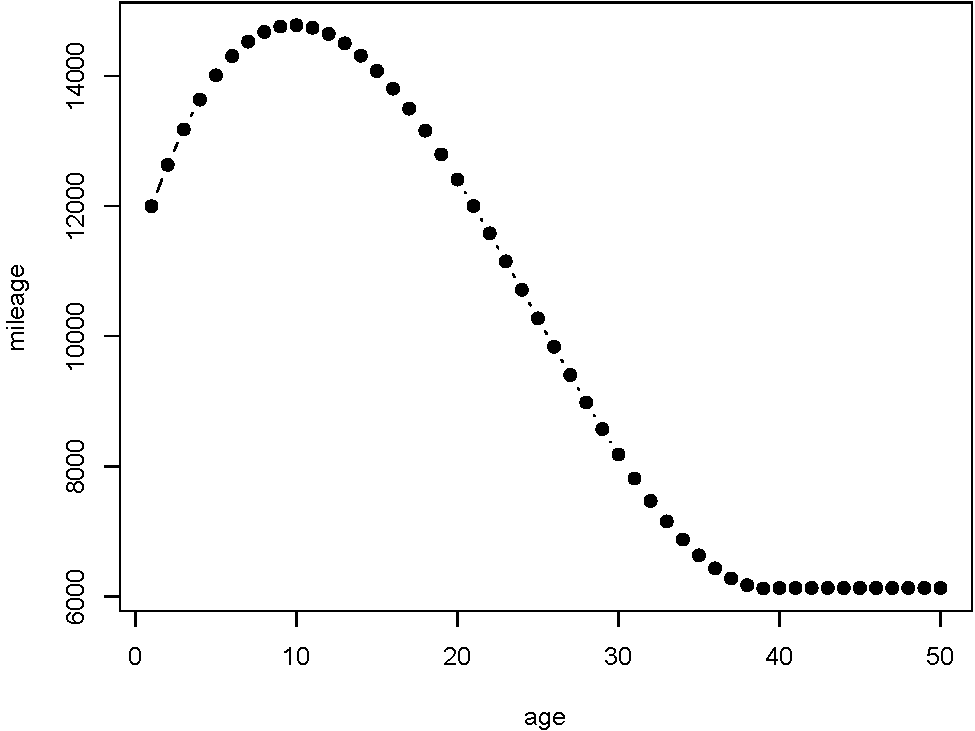
\includegraphics[width=0.8\linewidth]{veinbook_files/figure-latex/mil-1} 

}

\caption{Mileage of PC using E25}\label{fig:mil}
\end{figure}

\begin{itemize}
\tightlist
\item
  \textbf{net}: Road network of the west part of Sao Paulo city. It
  consistes in a SpatialLinesDataFrame (class of sp) with the attributes
  ldv (light duty vehicles, \(1 \cdot h^{-1}\)), hdv (heavy duty
  vehicles, \(1 \cdot h^{-1}\)), ps (peak speed, \(km \cdot h^{-1}\)),
  ffs (free flow speed, \(km \cdot h^{-1}\)), tstreet (type of street),
  lanes (number of lanes), capacity (capacity fo vehicles at each link,
  1/h) and tmin (time for travelling each link, min). The Fig.
  (\ref{traffic} shows more details.
\end{itemize}

\subsection{Temporal factors for Passenger
Cars}\label{temporal-factors-for-passenger-cars}

Temporal factors (TF) are the matrix of hourly traffic data normalized
for the hour of interest, usually the morning rush hour 08:00-09:00 in
local time (LT) \citep{gmd-2017-193}. This dataset covers 168 hours of
one week, from traffic counts of toll stations near the center of the
city of SãoPaulo, Brazil. Fig. (\ref{fig:tf} shows the temporal factors
for PC.

usage:

\begin{Shaded}
\begin{Highlighting}[]
\KeywordTok{library}\NormalTok{(vein, }\DataTypeTok{quietly =}\NormalTok{ T)}
\KeywordTok{data}\NormalTok{(pc_profile)}
\NormalTok{tf <-}\StringTok{ }\KeywordTok{unlist}\NormalTok{(pc_profile)}
\NormalTok{hours <-}\StringTok{ }\DecValTok{1}\OperatorTok{:}\DecValTok{168}
\KeywordTok{par}\NormalTok{(}\DataTypeTok{mar =} \KeywordTok{c}\NormalTok{(}\DecValTok{4}\NormalTok{, }\DecValTok{4}\NormalTok{, }\FloatTok{.1}\NormalTok{, }\FloatTok{.1}\NormalTok{))}
\KeywordTok{plot}\NormalTok{(}\DataTypeTok{y =}\NormalTok{ tf, }\DataTypeTok{x =}\NormalTok{ hours, }\DataTypeTok{pch =} \DecValTok{16}\NormalTok{, }\DataTypeTok{type =} \StringTok{"b"}\NormalTok{)}
\end{Highlighting}
\end{Shaded}

\begin{figure}

{\centering 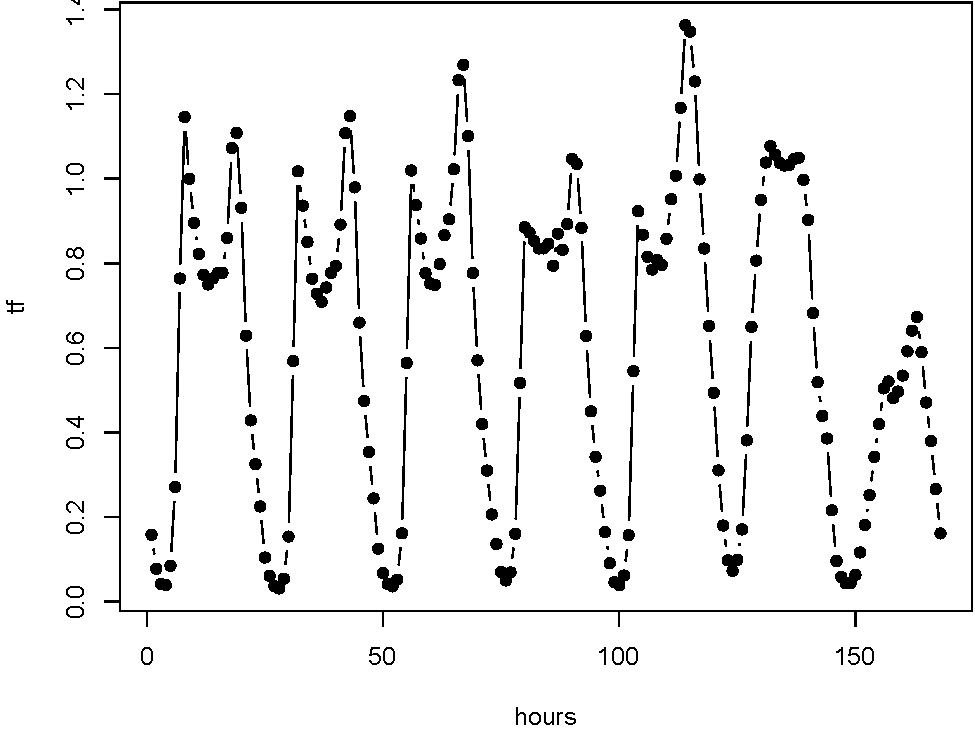
\includegraphics[width=0.8\linewidth]{veinbook_files/figure-latex/tf-1} 

}

\caption{Temporal Factors for PC}\label{fig:tf}
\end{figure}

\subsection{Profile for cold starts of Passenger
Cars}\label{profile-for-cold-starts-of-passenger-cars}

I included a profile of hourly percentage of cold starts of Passenger
Cars. This data covers 24 hours of a working day, and it is based cold
start recordings during the implementation of the International Vehicle
Emissions (IVE) model \citep{Davisetal2005} in São Paulo \citep{ivesp}.
The Fig. (\ref{fig:cold} shows the cold-start profile.

usage:

\begin{Shaded}
\begin{Highlighting}[]
\KeywordTok{library}\NormalTok{(vein, }\DataTypeTok{quietly =}\NormalTok{ T)}
\KeywordTok{data}\NormalTok{(pc_cold)}
\NormalTok{cold <-}\StringTok{ }\KeywordTok{unlist}\NormalTok{(pc_cold)}
\NormalTok{hours <-}\StringTok{ }\DecValTok{1}\OperatorTok{:}\DecValTok{24}
\KeywordTok{par}\NormalTok{(}\DataTypeTok{mar =} \KeywordTok{c}\NormalTok{(}\DecValTok{4}\NormalTok{, }\DecValTok{4}\NormalTok{, }\FloatTok{.1}\NormalTok{, }\FloatTok{.1}\NormalTok{))}
\KeywordTok{plot}\NormalTok{(}\DataTypeTok{y =}\NormalTok{ cold, }\DataTypeTok{x =}\NormalTok{ hours, }\DataTypeTok{pch =} \DecValTok{16}\NormalTok{, }\DataTypeTok{type =} \StringTok{"b"}\NormalTok{)}
\end{Highlighting}
\end{Shaded}

\begin{figure}

{\centering 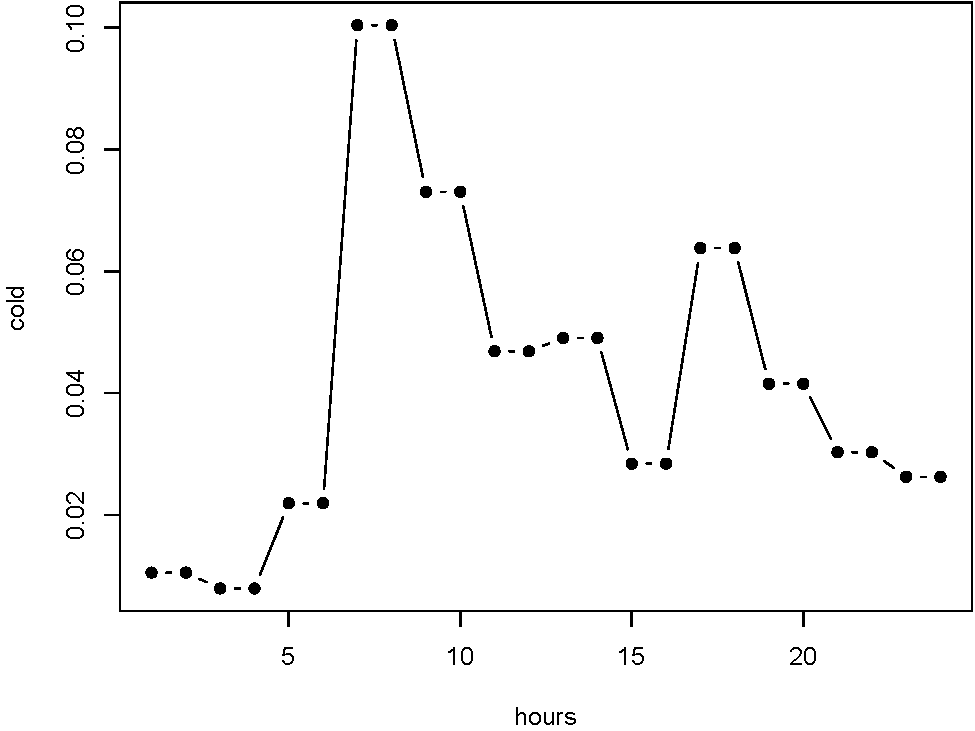
\includegraphics[width=0.8\linewidth]{veinbook_files/figure-latex/cold-1} 

}

\caption{Cold-starts profile for PC}\label{fig:cold}
\end{figure}

\section{Acknowledgements}\label{acknowledgements}

Martin Ramacher, Ph.D.~Student Chemistry Transport Modelling, Institute
for Coastal Research, Helmholtz-Zentrum Geesthacht, Germany -
Proofreading. Leila Droprinchinski Martins, Professor (Associate)
Federal Technological University of Parana, Brazil - Comments.

\chapter{Basics of R}\label{basic}

\section{Brief history}\label{brief-history}

R is a programming language developed by Ross Ihaka and Robert Genleman
in 1993 \citep{ihaka1996r}. An excellent resource about R is the book
``Programming for data science'' \citep{peng2015r}. R is like a free
version of S-PLUS programming language
(\url{http://www.solutionmetrics.com.au/products/splus/default.html}).
It is free and recognized as GNU software
(\url{https://www.gnu.org/software/software.html}) with GNU General
Public License (GPLV2-GPLV3) license. This feature allowed that many
developers started improving and adding code over the years.

R includes several statistical functions; therefore, users who want to
use the base capabilities of R are not forced to learn R-programming.
However, the evolution from user to developer in R has been facilitated
with numerous publications such as the book ``R packages: organize,
test, document, and share your code'' \citep{wickham2015r}, or ``The art
of R programming: A tour of statistical software design''
\citep{matloff2011art}.

\subsection{Installation}\label{installation-1}

R can be installed in different OS including Linux, Windows, Mac, and
Solaris. The webpage \url{https://cran.r-project.org/} shows how to
install R in any platform. A modern Integrated development environment
(IDE) is \textbf{RStudio} \url{https://www.rstudio.com/}, which contains
many useful integrated options. However, you can run R on the terminal,
and use any text editor to write and save scripts in R. Even more, you
can run R scripts on the terminal by typing
\texttt{Rscript\ -e\ "YourScript.R"}.

\section{Using R}\label{using-r}

If we type at the R promt

\begin{Shaded}
\begin{Highlighting}[]
\NormalTok{x <-}\StringTok{ }\DecValTok{1}   \CommentTok{# Not printing  results}
\NormalTok{x        }\CommentTok{# Print results}
\end{Highlighting}
\end{Shaded}

\begin{verbatim}
## [1] 1
\end{verbatim}

\begin{Shaded}
\begin{Highlighting}[]
\KeywordTok{print}\NormalTok{(x) }\CommentTok{# Explicit print x}
\end{Highlighting}
\end{Shaded}

\begin{verbatim}
## [1] 1
\end{verbatim}

The integer 1 was \emph{assigned} (\textless{}-) to x, then writing x or
print(x) shows the value of x. Instead of numbers, other expressions
such as strings, dates or other objects can n be assigned. R includes
several statistical functions. For instance, if we type `pi' at the
terminal, it prints the \emph{pi} number.

\begin{Shaded}
\begin{Highlighting}[]
\NormalTok{pi}
\end{Highlighting}
\end{Shaded}

\begin{verbatim}
## [1] 3.141593
\end{verbatim}

\subsection{R objects}\label{r-objects}

There are five basic classes (or atomic classes).

\begin{itemize}
\tightlist
\item
  character.
\item
  numeric.
\item
  integer.
\item
  complex.
\item
  logical (TRUE/FALSE or just T or F).
\end{itemize}

Objects of the same class can be grouped in \textbf{vectors}. You can
createVectors are created with writing\textbf{c()} with the elements of
the vector inside the parenthesis, separated by a colon. \textbf{c} is a
built-in function to create vectors. In this case, the vector v1
contains a sequence of three integers, from 1 to 3. The resulting class
is numeric.

\begin{Shaded}
\begin{Highlighting}[]
\NormalTok{v1 <-}\StringTok{ }\DecValTok{1}\OperatorTok{:}\DecValTok{3}
\NormalTok{v2 <-}\StringTok{ }\KeywordTok{c}\NormalTok{(}\DecValTok{1}\NormalTok{, }\DecValTok{2}\NormalTok{, }\DecValTok{3}\NormalTok{)}
\KeywordTok{identical}\NormalTok{(v1, v2)}
\end{Highlighting}
\end{Shaded}

\begin{verbatim}
## [1] FALSE
\end{verbatim}

\begin{Shaded}
\begin{Highlighting}[]
\NormalTok{v1}
\end{Highlighting}
\end{Shaded}

\begin{verbatim}
## [1] 1 2 3
\end{verbatim}

\begin{Shaded}
\begin{Highlighting}[]
\KeywordTok{class}\NormalTok{(v1)}
\end{Highlighting}
\end{Shaded}

\begin{verbatim}
## [1] "integer"
\end{verbatim}

With the operator \texttt{{[}} we can get specific elements of your
vectors. In the following code, the function \texttt{length} is used
additionally, which returns the length of an object.

\begin{Shaded}
\begin{Highlighting}[]
\NormalTok{v1[}\DecValTok{1}\NormalTok{]          }\CommentTok{# first element of v1}
\end{Highlighting}
\end{Shaded}

\begin{verbatim}
## [1] 1
\end{verbatim}

\begin{Shaded}
\begin{Highlighting}[]
\NormalTok{v1[}\KeywordTok{length}\NormalTok{(v1)] }\CommentTok{# last element element of v1}
\end{Highlighting}
\end{Shaded}

\begin{verbatim}
## [1] 3
\end{verbatim}

If we create a vector with numbers and letter, the resulting vector will
be ``character'', automatically converting the numbers into characters.

\begin{Shaded}
\begin{Highlighting}[]
\NormalTok{v2 <-}\StringTok{ }\KeywordTok{c}\NormalTok{(}\DecValTok{1}\OperatorTok{:}\DecValTok{3}\NormalTok{,}\StringTok{"a"}\NormalTok{)}
\NormalTok{v2}
\end{Highlighting}
\end{Shaded}

\begin{verbatim}
## [1] "1" "2" "3" "a"
\end{verbatim}

\begin{Shaded}
\begin{Highlighting}[]
\KeywordTok{class}\NormalTok{(v2)}
\end{Highlighting}
\end{Shaded}

\begin{verbatim}
## [1] "character"
\end{verbatim}

Objects can be converted to other classes with the as.* functions. For
instance, if we convert the vector v2 to numeric, it recognizes the
numbers adding an NA into the position of the character.

\begin{Shaded}
\begin{Highlighting}[]
\KeywordTok{as.numeric}\NormalTok{(v2)}
\end{Highlighting}
\end{Shaded}

\begin{verbatim}
## Warning: NAs introduzidos por coerção
\end{verbatim}

\begin{verbatim}
## [1]  1  2  3 NA
\end{verbatim}

\subsection{Factors}\label{factors}

Factors represent categorical data. A typical example is a character
vector of days of the week. The function \texttt{factor} creates
factors. To see the help section, type \texttt{?factor}. The following
example uses this function with the arguments \texttt{x} and
\texttt{levels}.

\begin{Shaded}
\begin{Highlighting}[]
\NormalTok{dow <-}\StringTok{ }\KeywordTok{factor}\NormalTok{(}\DataTypeTok{x =} \KeywordTok{c}\NormalTok{(}\StringTok{"Wednesday"}\NormalTok{, }\StringTok{"Monday"}\NormalTok{, }\StringTok{"Thursday"}\NormalTok{, }\StringTok{"Friday"}\NormalTok{),}
              \DataTypeTok{levels =}  \KeywordTok{c}\NormalTok{(}\StringTok{"Monday"}\NormalTok{, }\StringTok{"Tuesday"}\NormalTok{, }\StringTok{"Wednesday"}\NormalTok{, }\StringTok{"Thursday"}\NormalTok{,}
                          \StringTok{"Friday"}\NormalTok{))}
\NormalTok{dow}
\end{Highlighting}
\end{Shaded}

\begin{verbatim}
## [1] Wednesday Monday    Thursday  Friday   
## Levels: Monday Tuesday Wednesday Thursday Friday
\end{verbatim}

\subsection{Missing Values}\label{missing-values}

Missing values in data-sets are a typical source of a headache for R
users. Fortunately, R counts with several tools to avoid these
headaches. These tools are the functions \texttt{is.na} to check for NA
(not available) and \texttt{is.nan} (not a number). This function
returns logical values.

\begin{Shaded}
\begin{Highlighting}[]
\NormalTok{n <-}\StringTok{ }\KeywordTok{c}\NormalTok{(}\DecValTok{1}\NormalTok{, }\OtherTok{NA}\NormalTok{)}
\KeywordTok{is.na}\NormalTok{(n)}
\end{Highlighting}
\end{Shaded}

\begin{verbatim}
## [1] FALSE  TRUE
\end{verbatim}

\begin{Shaded}
\begin{Highlighting}[]
\NormalTok{n <-}\StringTok{ }\KeywordTok{c}\NormalTok{(}\DecValTok{1}\NormalTok{, }\OtherTok{NaN}\NormalTok{)}
\KeywordTok{is.na}\NormalTok{(n)}
\end{Highlighting}
\end{Shaded}

\begin{verbatim}
## [1] FALSE  TRUE
\end{verbatim}

\begin{Shaded}
\begin{Highlighting}[]
\KeywordTok{is.nan}\NormalTok{(n)}
\end{Highlighting}
\end{Shaded}

\begin{verbatim}
## [1] FALSE  TRUE
\end{verbatim}

\subsection{Matrices}\label{matrices}

Matrix is a structure with rows and columns. They can be created using
the \texttt{matrix} function and also, using vectors. Remember, if you
want to know more about any function you have to type \textbf{?} and the
function (e.g. \texttt{?matrix}), which opens the help documentation
page.

Let's create a matrix using vectors:

\begin{Shaded}
\begin{Highlighting}[]
\NormalTok{a <-}\StringTok{ }\DecValTok{1}\OperatorTok{:}\DecValTok{12}  \CommentTok{#numeric vector}
\NormalTok{(m <-}\StringTok{ }\KeywordTok{matrix}\NormalTok{(}\DataTypeTok{data =}\NormalTok{ a, }\DataTypeTok{nrow =} \DecValTok{3}\NormalTok{, }\DataTypeTok{ncol =} \DecValTok{4}\NormalTok{))}
\end{Highlighting}
\end{Shaded}

\begin{verbatim}
##      [,1] [,2] [,3] [,4]
## [1,]    1    4    7   10
## [2,]    2    5    8   11
## [3,]    3    6    9   12
\end{verbatim}

We can check the dimensions of our matrix \texttt{m} with \texttt{dim},
which are 3 and 4.

\begin{Shaded}
\begin{Highlighting}[]
\KeywordTok{dim}\NormalTok{(m)}
\end{Highlighting}
\end{Shaded}

\begin{verbatim}
## [1] 3 4
\end{verbatim}

In order to get the elements of matrix \texttt{m} we can use the
\texttt{{[}} operator:

\begin{Shaded}
\begin{Highlighting}[]
\NormalTok{m[}\DecValTok{1}\NormalTok{, }\DecValTok{1}\NormalTok{] }\CommentTok{# first element}
\end{Highlighting}
\end{Shaded}

\begin{verbatim}
## [1] 1
\end{verbatim}

\begin{Shaded}
\begin{Highlighting}[]
\NormalTok{m[, }\DecValTok{1}\NormalTok{]  }\CommentTok{# firs column}
\end{Highlighting}
\end{Shaded}

\begin{verbatim}
## [1] 1 2 3
\end{verbatim}

\begin{Shaded}
\begin{Highlighting}[]
\NormalTok{m[}\DecValTok{1}\NormalTok{, ]  }\CommentTok{# firs row}
\end{Highlighting}
\end{Shaded}

\begin{verbatim}
## [1]  1  4  7 10
\end{verbatim}

\begin{Shaded}
\begin{Highlighting}[]
\NormalTok{m[}\DecValTok{3}\NormalTok{,}\DecValTok{4}\NormalTok{]  }\CommentTok{# last element}
\end{Highlighting}
\end{Shaded}

\begin{verbatim}
## [1] 12
\end{verbatim}

\subsection{Arrays}\label{arrays}

Arrays are like matrices inside other matrices. A matrix is a
2-dimensional array. Let's create an array create an array using the
same vector \texttt{a} and same dimensions of \texttt{m}, 3 and 4.
\texttt{array} has three arguments, \texttt{data}, \texttt{dim} and
\texttt{dimnames}. In the argument \texttt{dim} let's add the number 2,
resulting in an array of two matrices identical to \texttt{m}.

\begin{Shaded}
\begin{Highlighting}[]
\NormalTok{(a <-}\StringTok{ }\KeywordTok{array}\NormalTok{(}\DataTypeTok{data =}\NormalTok{ a, }\DataTypeTok{dim =} \KeywordTok{c}\NormalTok{(}\DecValTok{3}\NormalTok{,}\DecValTok{4}\NormalTok{,}\DecValTok{2}\NormalTok{)))}
\end{Highlighting}
\end{Shaded}

\begin{verbatim}
## , , 1
## 
##      [,1] [,2] [,3] [,4]
## [1,]    1    4    7   10
## [2,]    2    5    8   11
## [3,]    3    6    9   12
## 
## , , 2
## 
##      [,1] [,2] [,3] [,4]
## [1,]    1    4    7   10
## [2,]    2    5    8   11
## [3,]    3    6    9   12
\end{verbatim}

We can subset elements from array also with the \texttt{{[}} operator.

\begin{Shaded}
\begin{Highlighting}[]
\NormalTok{a[}\DecValTok{1}\NormalTok{, }\DecValTok{1}\NormalTok{, }\DecValTok{1}\NormalTok{] }\CommentTok{# first element}
\end{Highlighting}
\end{Shaded}

\begin{verbatim}
## [1] 1
\end{verbatim}

\begin{Shaded}
\begin{Highlighting}[]
\KeywordTok{dim}\NormalTok{(a)     }\CommentTok{# dimensions}
\end{Highlighting}
\end{Shaded}

\begin{verbatim}
## [1] 3 4 2
\end{verbatim}

\begin{Shaded}
\begin{Highlighting}[]
\NormalTok{a[}\DecValTok{3}\NormalTok{, }\DecValTok{4}\NormalTok{, }\DecValTok{2}\NormalTok{] }\CommentTok{# last element}
\end{Highlighting}
\end{Shaded}

\begin{verbatim}
## [1] 12
\end{verbatim}

\subsection{Lists}\label{lists}

List are objects that can contain elements of different classes. I like
to call lists as bags. In a bag, you can put almost anything. Also,
inside the bag, you can put other bags with different things, meaning
that you can have a list of lists of any R object. You can create lists
with the \texttt{list} function. Let's create an empty list. Then I'm
using the vector \texttt{a} to create another list.

\begin{Shaded}
\begin{Highlighting}[]
\NormalTok{a <-}\StringTok{ }\DecValTok{1}\OperatorTok{:}\DecValTok{3}          \CommentTok{# vector of three elements}
\NormalTok{l1 <-}\StringTok{ }\KeywordTok{list}\NormalTok{()      }\CommentTok{# empty list}
\NormalTok{l1 <-}\StringTok{ }\KeywordTok{list}\NormalTok{(a)     }\CommentTok{# vector of three elements}
\KeywordTok{length}\NormalTok{(l1)        }\CommentTok{# length 1}
\end{Highlighting}
\end{Shaded}

\begin{verbatim}
## [1] 1
\end{verbatim}

\begin{Shaded}
\begin{Highlighting}[]
\NormalTok{l1 <-}\StringTok{ }\KeywordTok{as.list}\NormalTok{(a)  }\CommentTok{# vector a as list}
\KeywordTok{length}\NormalTok{(l1)        }\CommentTok{# three elements }
\end{Highlighting}
\end{Shaded}

\begin{verbatim}
## [1] 3
\end{verbatim}

As mentioned, the list can have lists inside.

\begin{Shaded}
\begin{Highlighting}[]
\NormalTok{l1 <-}\StringTok{ }\KeywordTok{list}\NormalTok{(}\KeywordTok{list}\NormalTok{(a),                    }\CommentTok{# three numeric elements}
            \KeywordTok{list}\NormalTok{(}\OtherTok{TRUE}\NormalTok{, }\OtherTok{TRUE}\NormalTok{, }\OtherTok{FALSE}\NormalTok{))   }\CommentTok{# three logical elements}
\KeywordTok{length}\NormalTok{(l1)                             }\CommentTok{# length 2}
\end{Highlighting}
\end{Shaded}

\begin{verbatim}
## [1] 2
\end{verbatim}

\subsection{Data-Frames}\label{data-frames}

``Data-frames are used to store tabular data in R'' \citep{peng2015r}.
You can think of data-frames as spreadsheet-like objects. They are
similar to matrices, and you can have a matrix and a data.frame with the
same dimensions. You have rows and columns, columns can have different
classes, and the columns usually have a one-word name.

Programmers, scientists, and practitioners use tabular data. Hence,
there are R packages created to extend the capabilities of the
data-frames. Below some of them:

\begin{itemize}
\tightlist
\item
  \texttt{data.frame} : This is not a package. It is a class and
  function from the \texttt{base} library in R. With this function you
  can create data-frames.
\item
  \texttt{data-table} \citep{datatable}: \texttt{data.tables} objects
  have the class \texttt{data.table} Which inherits from the class
  \texttt{data-frame}, which means that they share common
  characteristics. However, the big difference with \texttt{data-table}
  is the efficiency with memory. It includes functions such as
  \texttt{fread} for reading millions of observations in seconds.
\item
  \texttt{tidyr}\citep{tidyr}: Sometimes your data is in long format,
  and you need it in wide format, and vice-versa. This package does the
  job.
\item
  \texttt{readxl} \citep{readxl}: a Good package for importing Excel and
  LibreOffice files. I recommend this packages for newbies.
\item
  \texttt{sf} \citep{sf}: This package presents the class \texttt{sf}
  and introduces the list-column of spatial geometry.
\end{itemize}

Let's create a data.frame.

\begin{Shaded}
\begin{Highlighting}[]
\NormalTok{a <-}\StringTok{ }\DecValTok{1}\OperatorTok{:}\DecValTok{3}
\NormalTok{b <-}\StringTok{ }\DecValTok{3}\OperatorTok{:}\DecValTok{5}
\NormalTok{(ab <-}\StringTok{ }\KeywordTok{data.frame}\NormalTok{(a, b))}
\end{Highlighting}
\end{Shaded}

\begin{verbatim}
##   a b
## 1 1 3
## 2 2 4
## 3 3 5
\end{verbatim}

\begin{Shaded}
\begin{Highlighting}[]
\KeywordTok{class}\NormalTok{(ab)}
\end{Highlighting}
\end{Shaded}

\begin{verbatim}
## [1] "data.frame"
\end{verbatim}

\subsection{Names}\label{names}

In R you can put names in almost everything. Below examples for
\texttt{vectors}, \texttt{matrix} and \texttt{data.frames}.

\begin{Shaded}
\begin{Highlighting}[]
\KeywordTok{names}\NormalTok{(ab)                }\CommentTok{# original names}
\end{Highlighting}
\end{Shaded}

\begin{verbatim}
## [1] "a" "b"
\end{verbatim}

\begin{Shaded}
\begin{Highlighting}[]
\KeywordTok{names}\NormalTok{(ab) <-}\StringTok{ }\KeywordTok{c}\NormalTok{(}\StringTok{"c"}\NormalTok{, }\StringTok{"d"}\NormalTok{)}
\KeywordTok{names}\NormalTok{(ab)                }\CommentTok{# new names}
\end{Highlighting}
\end{Shaded}

\begin{verbatim}
## [1] "c" "d"
\end{verbatim}

\subsection{Subseting your data.frame}\label{subseting-your-data.frame}

There are several packages for filtering and manipulating data.frames
and databases, such as the famous \texttt{dplyr} \citep{dplyr}. However,
I will mention an essential characteristic to filter data.frames, and it
is not necessary for any new package, consisted in subsetting using
indices. Recall that data.frames are similar matrices, and you can
select values with this structure: \emph{{[}rows, columns{]}}.

Let's create a data.frame with three columns and select all commons that
match criteria for a row. Specifically, the column a fas rows with
values equal of 2

\begin{verbatim}
df <- data.frame(a = 1:3, b = 4:6, c = 7:9)
(aa <- df[df$a == 2,])
class(aa)
\end{verbatim}

here we are selecting all columns and the class of \texttt{aa} is
\texttt{data.frame}. The same applies for selecting columns, lets select
the columns ``b'' and ``c''.

\begin{verbatim}
(df[, c("b", "c")])
\end{verbatim}

\section{Inputting data into R}\label{inputting-data-into-r}

Your data can be in different formats. In this section, I'm showing you
how you can input text and comma separated value files, which is a
ubiquitous task. Let's say that you are using a spreadsheet program such
as Microsoft Excel or LibreOffice. Then you might want to import your
data into R.

\begin{itemize}
\tightlist
\item
  Your first check is if the first row of your data has a name or not.
  If they do have names, this means that they have a header.
\item
  Then click on `Save as' and search text file with extension .txt or
  .csv.
\item
  Then you edit your file with notepad (e.g., bloc, gedit, vi or another
  tool) to check if the decimal character is a point `.' so the
  separator character is a comma `,' or semicolon `;' or another
  character, which depends on the local configuration of your
  spreadsheet software.
\item
  If your file has the extension `.txt', use \texttt{read.table} and if
  it is `.csv', use \texttt{read.csv}.
\end{itemize}

Once you checked the format, you can import your `.txt' or `.csv' files
in R:

\begin{Shaded}
\begin{Highlighting}[]
\NormalTok{a <-}\StringTok{ }\KeywordTok{read.csv}\NormalTok{(}\StringTok{"path/to/file.csv"}\NormalTok{, }\DataTypeTok{sep =} \StringTok{","}\NormalTok{,}
              \DataTypeTok{header =}\NormalTok{ T, }\DataTypeTok{stringsAsFactors =}\NormalTok{ F)}
\NormalTok{a <-}\StringTok{ }\KeywordTok{read.table}\NormalTok{(}\StringTok{"path/to/file.txt"}\NormalTok{, }\DataTypeTok{sep =} \StringTok{","}\NormalTok{,}
                \DataTypeTok{header =}\NormalTok{ T, }\DataTypeTok{stringsAsFactors =}\NormalTok{ F)}
\end{Highlighting}
\end{Shaded}

\chapter{Structuring an Emissions Inventory}\label{st}

The elaboration of vehicular emissions inventories in VEIN consists of
four stages:

\begin{enumerate}
\def\labelenumi{\arabic{enumi}.}
\tightlist
\item
  pre-processing activity data,
\item
  preparing emissions factors,
\item
  estimating the emissions and
\item
  post-processing of emissions in maps and databases.
\end{enumerate}

VEIN provides functions to each of the stages. However, to follow these
stages, a structure of directories with scripts including vein functions
is necessary. Therefore, the vein function \texttt{inventory} creates
this structure of directories.

\section{Overview of emissions inventorying using
VEIN}\label{veinstructure}

\begin{figure}

{\centering 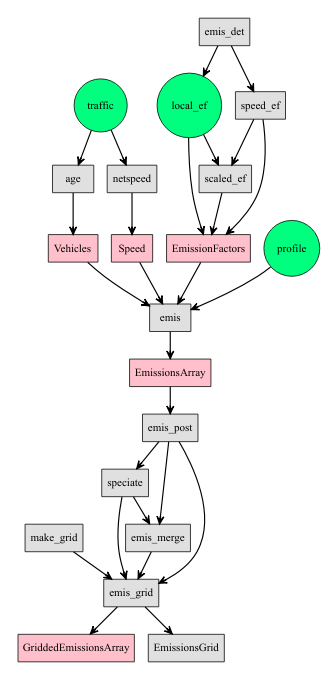
\includegraphics[width=0.7\linewidth]{figuras/dia1} 

}

\caption{Structuring an emissions inventories with VEIN}\label{fig:diavein}
\end{figure}

\section{\texorpdfstring{The \texttt{inventory}
function}{The inventory function}}\label{the-inventory-function}

The inventory function creates a structure of directories and scripts to
run VEIN. This structure is a suggestion, and the user can use any
other. The following code shows the arguments of the function using the
\texttt{args} function with \texttt{inventory}.

\begin{Shaded}
\begin{Highlighting}[]
\KeywordTok{args}\NormalTok{(inventory)}
\end{Highlighting}
\end{Shaded}

\begin{verbatim}
## function (name, vehcomp = c(PC = 1, LCV = 1, HGV = 1, BUS = 1, 
##     MC = 1), show.main = TRUE, scripts = TRUE, show.dir = TRUE, 
##     show.scripts = FALSE, clear = TRUE, rush.hour = FALSE) 
## NULL
\end{verbatim}

The arguments are \texttt{name}, \texttt{vehcomp}, \texttt{show.main},
\texttt{scripts}, \texttt{show.dir}, \texttt{show.scripts} and
\texttt{clear}.

\begin{itemize}
\tightlist
\item
  The argument \texttt{name}
\end{itemize}

The argument name is a word to be used as the main directory where
directories and scripts are stored. It consists in \emph{one} word with
ASCII characters. It is also recommended to exclude any special
character or accents, for instance:

\begin{Shaded}
\begin{Highlighting}[]
\NormalTok{name =}\StringTok{ }\KeywordTok{file.path}\NormalTok{(}\KeywordTok{tempdir}\NormalTok{(), }\StringTok{"YourCity"}\NormalTok{)}
\KeywordTok{inventory}\NormalTok{(}\DataTypeTok{name =}\NormalTok{ name,  }\DataTypeTok{show.dir =} \OtherTok{TRUE}\NormalTok{, }\DataTypeTok{show.scripts =} \OtherTok{TRUE}\NormalTok{)}
\end{Highlighting}
\end{Shaded}

\begin{itemize}
\tightlist
\item
  The argument \texttt{vehcomp} This argument is critical and comes from
  \emph{Vehicular Composition}, which is the classification of the fleet
  by type of use, type of fuel, size of engine and gross weight, based
  on definitions of \citet{Corvalanetal2002}. There is also the
  \emph{technological composition} of the fleet which relates the
  technological modifications of the car to accomplish the emissions
  standards. However, vein uses a distribution by the age of use as
  \ref{traffic} shows.
\end{itemize}

The vehicular composition \texttt{vehcomp} has 5 types of vehicles:

\begin{enumerate}
\def\labelenumi{\arabic{enumi}.}
\tightlist
\item
  Passenger Cars (PC).
\item
  Light Commercial Vehicles (LCV).
\item
  Heavy Good Vehicles or trucks (HGV).
\item
  Buses (BUS).
\item
  Motorcycles (MC).
\end{enumerate}

The default value of this argument is:
\texttt{c(PC\ =\ 1,\ LCV\ =\ 1,\ HGV\ =\ 1,\ BUS\ =\ 1,\ MC\ =\ 1)},
which means that there are 1 types of PC, 1 of LCV, 1 of trucks, 1 of
buses and 1 types of motorcycles. This vehicular composition is only for
illustrating that the user can change these values according to its
data. Appendix B shows the vehicular composition from the vehicular
emissions inventory of the Environmental Agency of São Paulo, Brazil
\citep{CETESB2015}. In Brazil, the fuel used in vehicles is blended with
ethanol with and biodiesel. The user can use \textbf{any} vehicular
composition that represents its fleet with up to 99 types of vehicles
per category. For instance, if there are 4 types of PC in a fleet,
\texttt{PC\ =\ 4}, and each one has aa age of use distribution.

\begin{itemize}
\tightlist
\item
  The argument \texttt{scripts}
\end{itemize}

This argument adds scripts into the directories. The default is TRUE.
The type of scripts create are:

\begin{itemize}
\item
  main.R: Adds the \texttt{setwd("YourCity")}, \texttt{library(vein)},
  \texttt{source(traffic.R)}, some comments and a loop to source all
  inputs. It is recommended not using the loop till it is certain that
  all scripts are correct.
\item
  traffic.R: Includes two lines with examples of how to use the
  \texttt{age\_ldv} function and saving the output in the directory veh.
\item
  input.R: Each file has the scripts for reading the network, vehicles,
  emission factors and estimating emissions.
\item
  The argument \texttt{show.main}
\end{itemize}

This argument is to open automatically the file main.R. Default value is
TRUE.

\begin{itemize}
\tightlist
\item
  The argument \texttt{show.dir}
\end{itemize}

This is a logical argument to decide if the output of the function will
return print the new directories or not. The use is:

\begin{Shaded}
\begin{Highlighting}[]
\NormalTok{name =}\StringTok{ }\KeywordTok{file.path}\NormalTok{(}\KeywordTok{tempdir}\NormalTok{(), }\StringTok{"YourCity"}\NormalTok{)}
\KeywordTok{inventory}\NormalTok{(}\DataTypeTok{name =}\NormalTok{ name, }\DataTypeTok{show.main =} \OtherTok{FALSE}\NormalTok{, }\DataTypeTok{show.dir =} \OtherTok{TRUE}\NormalTok{, }\DataTypeTok{show.scripts =} \OtherTok{FALSE}\NormalTok{)}
\end{Highlighting}
\end{Shaded}

\begin{verbatim}
files at /tmp/RtmpT5bNtr/YourCity
Directories:
 [1] "/tmp/RtmpT5bNtr/YourCity"              "/tmp/RtmpT5bNtr/YourCity/ef"          
 [3] "/tmp/RtmpT5bNtr/YourCity/emi"          "/tmp/RtmpT5bNtr/YourCity/emi/BUS_01"  
 [5] "/tmp/RtmpT5bNtr/YourCity/emi/HGV_01"   "/tmp/RtmpT5bNtr/YourCity/emi/LCV_01"  
 [7] "/tmp/RtmpT5bNtr/YourCity/emi/MC_01"    "/tmp/RtmpT5bNtr/YourCity/emi/PC_01"   
 [9] "/tmp/RtmpT5bNtr/YourCity/est"          "/tmp/RtmpT5bNtr/YourCity/images"      
[11] "/tmp/RtmpT5bNtr/YourCity/network"      "/tmp/RtmpT5bNtr/YourCity/post"        
[13] "/tmp/RtmpT5bNtr/YourCity/post/df"      "/tmp/RtmpT5bNtr/YourCity/post/grids"  
[15] "/tmp/RtmpT5bNtr/YourCity/post/streets" "/tmp/RtmpT5bNtr/YourCity/profiles"    
[17] "/tmp/RtmpT5bNtr/YourCity/veh"     
\end{verbatim}

\texttt{inventory} creates the directory ``YourCity'' and the
subdirectories: daily, ef, emi, est, images, network, and veh.

\begin{itemize}
\item
  \textbf{daily}: Directory for storing the profiles saved as .csv
  files. For instance, \texttt{data(pc\_profile)} is a matrix that could
  be saved as .csv.
\item
  \textbf{ef}: Directory for storing the emission factors data-frame,
  similar to \texttt{data(fe2015)} but including one column for each of
  the categories of the vehicular composition. For instance, if PC = 5,
  there should be 5 columns with emission factors in this file. If LCV =
  5, another 5 columns should be present, and so on.
\item
  \textbf{emi}: Directory with subdirectories matching the vehicular
  composition for saving the estimates. It is suggested to use .rds
  extension instead of .rda.
\item
  \textbf{est}: Directory with subdirectories matching the vehicular
  composition for storing the scripts named \texttt{input.R}.
\item
  \textbf{images}: Directory for saving images.
\item
  \textbf{network}: Directory for saving the road network with the
  required attributes. This file will include the vehicular flow per
  street to be used by functions \texttt{age\_ldv}, \texttt{age\_hdv},
  \texttt{age\_moto} or \texttt{my\_ldv}.
\item
  \textbf{post}: Directory for storing the processed emissions. It
  includes the directories \textbf{df} for emissions by the age of use,
  hour and other parameters, \textbf{streets} for storing the total
  emissions by streets and \textbf{grids} for storing total gridded
  emissions by pollutant.
\item
  \textbf{veh}: Directory for storing the distribution by the age of use
  of each category of the vehicular composition. Those are data-frames
  with each column as the age of use, and the number of rows as the
  number of streets. The class of these objects is ``Vehicles''.
\item
  The argument \texttt{show.scripts}
\end{itemize}

This argument prints the scripts created:

\begin{Shaded}
\begin{Highlighting}[]
\NormalTok{name =}\StringTok{ }\KeywordTok{file.path}\NormalTok{(}\KeywordTok{tempdir}\NormalTok{(), }\StringTok{"YourCity"}\NormalTok{)}
\KeywordTok{inventory}\NormalTok{(}\DataTypeTok{name =}\NormalTok{ name, }\DataTypeTok{show.main =} \OtherTok{FALSE}\NormalTok{, }\DataTypeTok{show.dir =} \OtherTok{FALSE}\NormalTok{, }\DataTypeTok{show.scripts =} \OtherTok{TRUE}\NormalTok{)}
\end{Highlighting}
\end{Shaded}

\begin{verbatim}
files at /tmp/RtmpT5bNtr/YourCity
Scripts:
[1] "est/BUS_01_input.R" "est/HGV_01_input.R" "est/LCV_01_input.R"
[4] "est/MC_01_input.R"  "est/PC_01_input.R"  "main.R"            
[7] "post.R"             "traffic.R"   
\end{verbatim}

\begin{itemize}
\tightlist
\item
  The argument \texttt{clear}
\end{itemize}

This is a logical argument that deletes recursively when TRUE, or not
when FALSE, the directory and creates another one. The default is TRUE.

The following chapters show the use of other vein functions inside a
structure of directories and scripts with the name
\texttt{inventory("YourCity")}.

\chapter{Traffic data}\label{traffic}

The traffic data can have different formats, but it is inherently
spatial data. Hence, traffic data must be in any \textbf{vectorial}
spatial format with the drivers provided by the library\textbf{GDAL}
(\url{http://www.gdal.org/ogr_formats.html}), using the package
\textbf{sf} \citep{sf}. Eventually, some traffic data can be distributed
in raster format, for instance, after some spatial interpolations. In
this case, I recommend using the function \texttt{grid\_emis} to
distribute the traffic of each cell into vectorial lines of streets, see
section @ref(\#post). The Eq. \eqref{eq:flow} shows how hourly traffic
data considered in VEIN.

\begin{equation}
F^*_{i,j,k} = Q_{i} \cdot VC_{i,j} \cdot Age_{j,k}
\label{eq:flow}
\end{equation}

where \(F^*_{i,j,k}\) is the vehicular flow at street link \(i\) for
vehicle type \(j\) by age of use \(k\). \(j\) defines the vehicular
composition according to its type of use, type of fuel, size of engine
and gross weight, based on definitions of \citep{Corvalanetal2002}.
\(Q_i\) is the traffic flow at street link \(i\). \(VC_{i,j}\) is the
fraction of vehicles varying according to the type of vehicles \(j\) in
the vehicle fleet at street link \(i\). \(Age_{j,k}\) is the age
distribution by vehicular composition \(j\) and age of use \(k\).

This Equation shows that \(VC\) splits the total vehicular flow \(Q\) to
identify the vehicular fraction, which varies according to the type of
fuel, size of motor and gross weight. For example, if \(Q\) is
light-duty vehicles (LDV) and it is known that 5\% of the \(Q\) are
passenger cars (PC), with engines lesser than 1400 cc, \(VC\) is 0.05.
This characterization of the fleet depends on the amount and quality of
the available information. VEIN then multiplies the traffic with \(Age\)
to obtain the amount of each type of vehicle by the age of use.

\section{Sources of traffic data}\label{sources-of-traffic-data}

\subsection{Travel demand outputs}\label{travel-demand-outputs}

VEIN was developed according to the available traffic data in São Paulo,
Brazil. In this case, the available data was a 4-stage macroscopic
travel model for morning rush hours and hourly traffic counts for
morning and evening rush hours. The travel model is based on data from
an Origin-Destination-Survey (ODS) \citep{ODS} which started in the
decade of 1950 in São Paulo. A classic reference of a 4-stage modeling
transport is \citep{OrtuzarWillumsen2002}. The 4 stages of the traffic
modeling include characterization of trip attractions and productions by
zone in some regions, distribution of these trips, the preferred mode of
transport for traveling and finally the allocation of the trips at each
mode; in this case into the road network. The ODS is made every 10 years
by Metro (\url{http://www.metro.sp.gov.br/}), which is the underground
company, and they perform a smaller update of ODS after 5 years. The
information gathered in the ODS is massive due to the participation of
thousands of commuters. It helps to identify the characteristics of the
trips inside MASP. CET uses the information from ODS and performs the
traffic simulation. In this case, it is a macro or strategic traffic
simulation which represents the equilibrium between offer and supply of
transportation at maximum load of the road network, that is, at the rush
hour, which is from 08:00 to 09:00 Local Time (LT).

VEIN incorporates an extract of a traffic model simulation for the west
part of São Paulo named \emph{net}. The Fig. (\ref{fig:ldv} shows the
traffic of Light-Duty Vehicles (LDV). This data covers the surrounding
area of the University of São Paulo. The information obtained from CET
consists in:

\begin{itemize}
\tightlist
\item
  \emph{ldv}: Light Duty Vehicles (1/h).
\item
  \emph{hdv}: Heavy Duty Vehicles (1/h).
\item
  \emph{lkm}: Length of the link (km).
\item
  \emph{ps}: Peak Speed (km/h).
\item
  \emph{ffs}: Free Flow Speed (km/h).
\item
  \emph{tstreet}: Type of street.
\item
  \emph{lanes}: Number of lanes per link.
\item
  \emph{capacity}: Capacity of vehicles in each link (1/h).
\item
  \emph{tmin}: Time for traveling each link (min).
\end{itemize}

The following scripts show how to load this data in R. This data has the
class ``SpatialLinesDataFrame'' from the package \citep{sp}. This data
was converted into a spatial feature ``sf'' object \citep{sf} because it
consists of a data-frame with a list-column of geometry with the spatial
attributes and it is easier to handle than an sp object class.

The user must call the library VEIN first, then load the data
\textbf{net}. The object net has the class ``SpatialLinesDataFrame''.
This data can be loaded and shown in R like this:

\begin{Shaded}
\begin{Highlighting}[]
\KeywordTok{library}\NormalTok{(vein)}
\KeywordTok{library}\NormalTok{(sp)}
\KeywordTok{data}\NormalTok{(net)}
\KeywordTok{class}\NormalTok{(net)}
\end{Highlighting}
\end{Shaded}

\begin{verbatim}
## [1] "SpatialLinesDataFrame"
## attr(,"package")
## [1] "sp"
\end{verbatim}

The Fig. (\ref{fig:ldv}) shows that traffic is concentrated in main
streets such as the motorway Marginal Pinheiros, located in the
northeast part of the area.

\begin{Shaded}
\begin{Highlighting}[]
\KeywordTok{library}\NormalTok{(vein)}
\KeywordTok{data}\NormalTok{(net)}
\NormalTok{net}\OperatorTok{$}\NormalTok{ldv <-}\StringTok{ }\KeywordTok{as.numeric}\NormalTok{(net}\OperatorTok{$}\NormalTok{ldv)}
\KeywordTok{spplot}\NormalTok{(net, }\StringTok{"ldv"}\NormalTok{, }\DataTypeTok{scales =} \KeywordTok{list}\NormalTok{(}\DataTypeTok{draw =}\NormalTok{ T),}
       \DataTypeTok{col.regions =} \KeywordTok{rev}\NormalTok{(}\KeywordTok{bpy.colors}\NormalTok{(}\DecValTok{16}\NormalTok{)))}
\end{Highlighting}
\end{Shaded}

\begin{figure}

{\centering 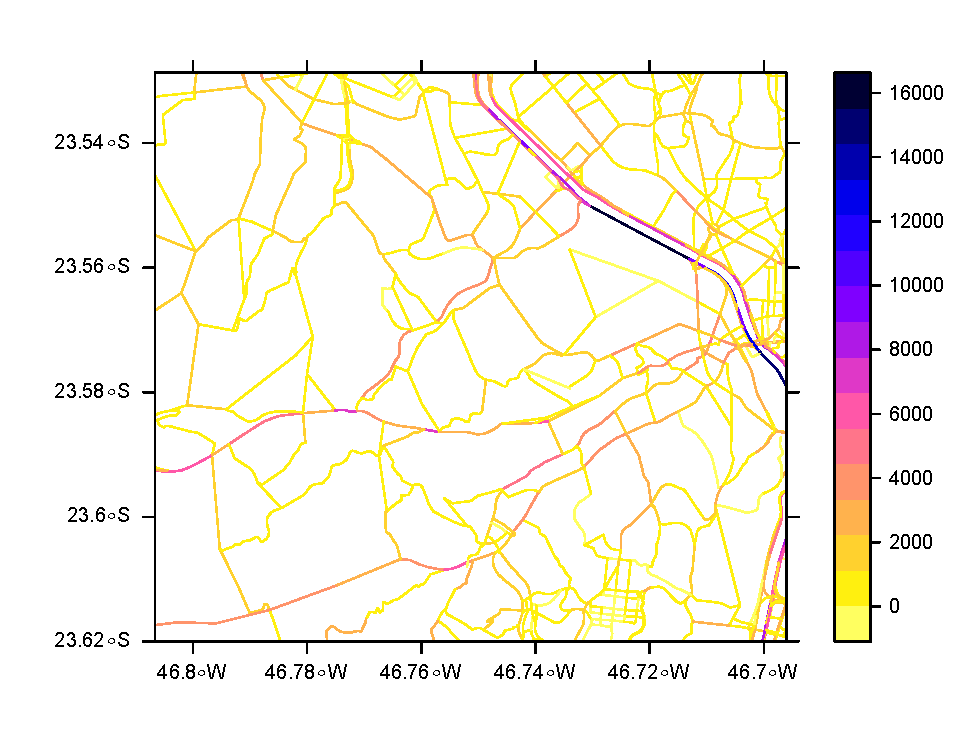
\includegraphics[width=0.8\linewidth]{veinbook_files/figure-latex/ldv-1} 

}

\caption{LDV at 08:00-09:00 (LT) in west São Paulo}\label{fig:ldv}
\end{figure}

\subsection{Interpolation of traffic
counts}\label{interpolation-of-traffic-counts}

Travel model simulations are not always available, and the user
interested in estimating vehicular emissions with a bottom-up approach
would have to look for alternatives to obtain traffic data at street
level. These alternatives cover interpolating traffic data for different
temporal resolutions. For instance, \citet{requia} developed a vehicular
bottom-up inventory using traffic counts and a geostatistic method
called Global Moran's I test \citep{anselin}. It measures the spatial
autocorrelation. However, this technique requires that the observed
values with a normal distribution, which is not the case for count data.

Other authors were interested in predicting Anual Average Daily Traffic
(AADT) or only ADT. \citet{lowry2014spatial} presented a new method for
predicting AADT based on the concept of origin-destination centrality.
The idea is to obtain predictor variables directly from the road
network. He identified origin and destination zones and added
multiplication factors based on the land-use characteristics.

\citet{zhao2001contributing} tested several multiple stepwise
regressions incorporating land-use characteristics. They considered
several variables: number of lanes, classification of road type,
employment numbers and access to expressway with correlations between
0.66 and 0.82. \citet{lam2000estimation} compared neural networks and
regressions for a dataset of 13 locations. Kriging methods were used in
AADT interpolation by \citet{eom2006improving}, who predicted AADT for
non-motorway streets. Also, \citet{selby2013spatial} compared Kriging
and geographically weighted regressions in the prediction of AADT.

Another approach is to perform a spatial regression based on the
distribution of the observed data. As the data are counts of traffic, a
Poisson, quasi-Poisson or negative binomial regressions can be used
\citep{zeileis2008regression}. Recently, \citet{Ibarraetal2017a}
compared quasi-Poisson and negative binomial regressions predicting
hourly traffic data, with better results for a quasi-Poisson approach
(correlation of 0.72).

Newer approaches involve GPS data from smartphones and cars.

\subsection{Generating traffic flows from Origin-Destination-Surveys
(ODS)}\label{generating-traffic-flows-from-origin-destination-surveys-ods}

The origin-destination survey (ODS) is an important tool which
quantifies the number of trips generated in the study area. ODS studies
started decades ago. The oldest ODS paper on Google Scholar is entitled
``FUNCTIONS OF A HIGHWAY-PLANNING SURVEY DEPARTMENT'' by W. J. Sapp in
1938 at the TWENTY-FOURTH ANNUAL ROAD SCHOOL \citep{sapp1938runctions}.
In this paper, the importance of information for the traffic engineer is
discussed: ``The engineer must have the supporting data available to
substantiate his decisions.''

Another study of 1942 shows the importance of traffic counts, discussing
The elaboration of an origin-destination survey where 8000 Boy Scouts of
America participated in counting traffic. The method for analyzing the
data consisted in counting the vehicles identifying the license plate to
determine the origin (the first time the vehicle was recorded), the
route of vehicles, the destination and the approximate time for the
trip.

After those pioneer studies, many many other studies went deeper into
the subject. Moreover, after that, with the irruption of new
technologies, new software, use of smartphones with GPS, satellites and
big technological centers owned by companies such as Google
(\url{http://www.google.com}), new ways for characterizing trips were
developed. In this section, I will briefly mention the Google Distance
Matrix
(\url{https://developers.google.com/maps/documentation/distance-matrix/}),
the pgRouting library \citep{patrushev2007shortest} for PostGIS and will
expand with two R packages, googleway \citep{googleway} and dodgr
\citep{dodgr}.

The ODS provides the matrix of pairs of zones origin and destinations by
mode of transport. Then, we can use any of the mentioned software to
find the shortest path between each zone. The table \ref{tab:ods} shows
extraction of the OD matrix for the Metropolitan Area of São Paulo
(MASP) in 2007 for individual motorized trips. The fig @ref(fig.zod)
shows a map with the location of the zones OD.

\begin{table}

\caption{\label{tab:ods}Matrix OD for motorized indivitual trips between 06:30 and 08:30 MASP 2007}
\centering
\begin{tabular}[t]{lcccccccccc}
\toprule
  & V101 & V102 & V103 & V104 & V105 & V106 & V107 & V108 & V109 & V110\\
\midrule
101 & 42 & 0 & 0 & 83 & 0 & 84 & 42 & 0 & 0 & 318\\
102 & 49 & 0 & 10 & 0 & 0 & 20 & 0 & 10 & 0 & 0\\
103 & 0 & 10 & 0 & 19 & 0 & 81 & 17 & 0 & 0 & 54\\
104 & 0 & 35 & 86 & 40 & 0 & 170 & 40 & 35 & 35 & 0\\
105 & 0 & 0 & 0 & 13 & 0 & 0 & 0 & 0 & 0 & 0\\
\addlinespace
106 & 94 & 0 & 72 & 87 & 24 & 196 & 15 & 0 & 0 & 27\\
107 & 0 & 0 & 13 & 64 & 13 & 28 & 44 & 0 & 0 & 0\\
108 & 0 & 0 & 0 & 0 & 0 & 0 & 0 & 3525 & 885 & 0\\
109 & 0 & 0 & 0 & 0 & 0 & 206 & 0 & 3916 & 975 & 0\\
110 & 954 & 0 & 18 & 954 & 0 & 0 & 0 & 652 & 939 & 2928\\
\bottomrule
\end{tabular}
\end{table}

\begin{figure}

{\centering 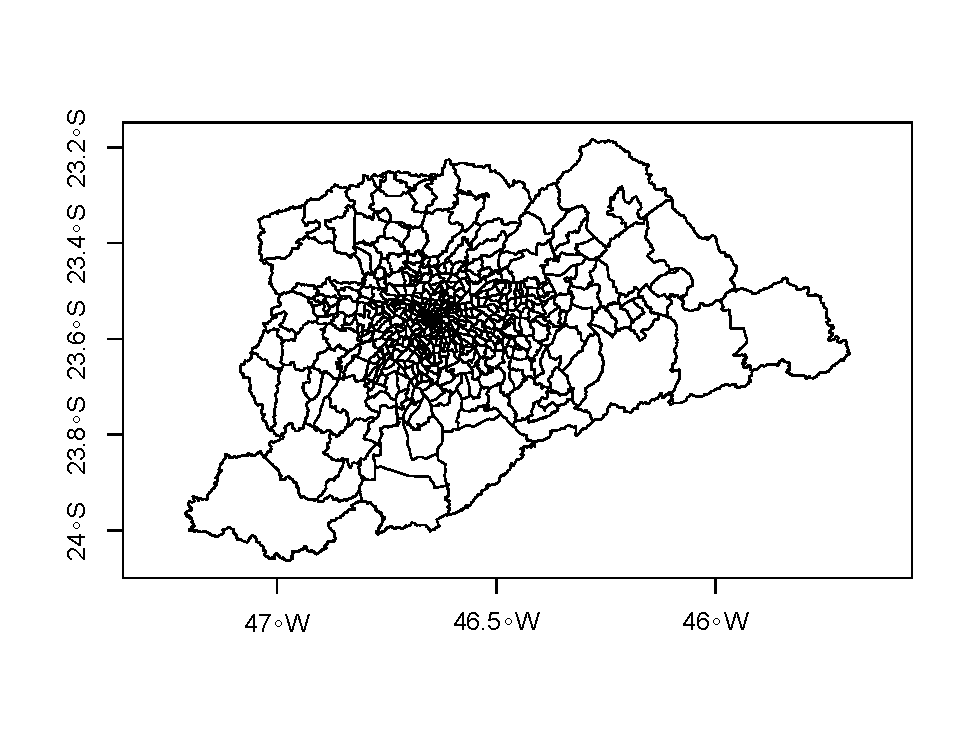
\includegraphics[width=1\linewidth]{veinbook_files/figure-latex/zod-1} 

}

\caption{Zones OD for MASP 2007}\label{fig:zod}
\end{figure}

Now, as we know the trips between each pair of OD zones, we can find the
routes that connect them. Algorithms are used to find the shortest path.
It connects two nodes minimizing the total travel time. There are
several algorithms, including \citet{dijkstra1959note}.

\subsubsection{Google Distance Matrix
API}\label{google-distance-matrix-api}

This service allows to ``retrieve duration and distance values based on
the recommended route between start and end points.'' It returns
durations and distance, and it is possible to choose modes of transport
as well as to choose between current or historical times. The first step
is to get a KEY.

If you browse

\begin{Shaded}
\begin{Highlighting}[]
\ExtensionTok{https}\NormalTok{://maps.googleapis.com/maps/api/distancematrix/json?units=imperial}\KeywordTok{&}\VariableTok{origins=}\NormalTok{Washington,DC}\KeywordTok{&}\VariableTok{destinations=}\NormalTok{New+York+City,NY}\KeywordTok{&}\VariableTok{key=}\NormalTok{YOUR_API_KEY}
\end{Highlighting}
\end{Shaded}

Replace YOUR\_API\_KEY (my browser is in Portuguese):

\begin{Shaded}
\begin{Highlighting}[]
\KeywordTok{\{}
  \StringTok{"destination_addresses"} \BuiltInTok{:}\NormalTok{ [ }\StringTok{"Nova York, NY, EUA"}\NormalTok{ ],}
  \StringTok{"origin_addresses"} \BuiltInTok{:}\NormalTok{ [ }\StringTok{"Washington, D.C., Distrito de Columbia, EUA"}\NormalTok{ ],}
  \StringTok{"rows"} \BuiltInTok{:}\NormalTok{ [}
    \KeywordTok{\{}
      \StringTok{"elements"} \BuiltInTok{:}\NormalTok{ [}
        \KeywordTok{\{}
          \StringTok{"distance"} \BuiltInTok{:}\NormalTok{ \{}
            \StringTok{"text"} \BuiltInTok{:} \StringTok{"225 mi"}\NormalTok{,}
            \StringTok{"value"} \BuiltInTok{:}\NormalTok{ 361972}
          \KeywordTok{\}}\NormalTok{,}
          \StringTok{"duration"} \BuiltInTok{:}\NormalTok{ \{}
            \StringTok{"text"} \BuiltInTok{:} \StringTok{"3 horas 53 minutos"}\NormalTok{,}
            \StringTok{"value"} \BuiltInTok{:}\NormalTok{ 13964}
          \KeywordTok{\}}\NormalTok{,}
          \StringTok{"status"} \BuiltInTok{:} \StringTok{"OK"}
        \KeywordTok{\}}
\NormalTok{        ]}
\NormalTok{    \}}
\NormalTok{    ],}
  \StringTok{"status"} \BuiltInTok{:} \StringTok{"OK"}
\NormalTok{\}}
\end{Highlighting}
\end{Shaded}

The modes of transport covered are \textbf{driving} using the road
network, \textbf{walking} via pedestrian paths \& sidewalks,
\textbf{bicycling} via bicycle paths and \textbf{transit} via public
transit routes. For more information read the documentation.

\subsubsection{pgRouting for postGIS}\label{pgrouting-for-postgis}

pgRouting (\url{http://pgrouting.org/}) is an open source routing
library for postGIS. It provides many routing algorithms, and it can be
run via QGIS (\url{https://www.qgis.org}). This library is very
extensive. An excellent resource is the book ``pgRouting: A Practical
Guide'' (\url{http://locatepress.com/pgrouting}).

\subsubsection{The R package googleway}\label{the-r-package-googleway}

googleway \citep{googleway} R package allows accessing Google Maps API
\url{https://developers.google.com/maps/}. The API functions are:

\begin{itemize}
\tightlist
\item
  Directions - \texttt{google\_directions()}
\item
  Distance Matrix - \texttt{google\_distance()}
\item
  Elevation - \texttt{google\_elevation()}
\item
  Geocoding - \texttt{google\_geocode()}
\item
  Reverse Geocoding - \texttt{google\_reverse\_geocode()}
\item
  Places - \texttt{google\_places()}
\item
  Place Details - \texttt{google\_place\_details()}
\item
  Time zone - \texttt{google\_timezone()}
\item
  Roads - \texttt{google\_snapToRoads()} and
  \texttt{google\_nearestRoads()}
\end{itemize}

This package allows plotting over Google Maps.

\begin{Shaded}
\begin{Highlighting}[]
\KeywordTok{library}\NormalTok{(googleway)}
\NormalTok{## not specifying the api will add the key as your 'default'}
\NormalTok{key <-}\StringTok{ "my_api_key"}
\KeywordTok{set_key}\NormalTok{(}\DataTypeTok{key =}\NormalTok{ key)}
\KeywordTok{google_keys}\NormalTok{()}
\end{Highlighting}
\end{Shaded}

\begin{verbatim}
## Google API keys
##  -  default : my_api_key 
##  -  map :  
##  -  directions :  
##  -  distance :  
##  -  elevation :  
##  -  geocode :  
##  -  places :  
##  -  find_place :  
##  -  place_autocomplete :  
##  -  place_details :  
##  -  reverse_geocode :  
##  -  roads :  
##  -  streetview :  
##  -  timezone :
\end{verbatim}

From zone Luz 7, coordinates long -46.63461 and lat -23.53137 to zone 8
Bom Retiro coordinates -46.64482 -23.52204 there are 133 LDV trips
between 6:30 and 08:30. We first create the data-frame. This data is
based on OD from São Paulo.

\begin{Shaded}
\begin{Highlighting}[]
\NormalTok{mydf <-}\StringTok{ }\KeywordTok{data.frame}\NormalTok{(}\DataTypeTok{region =} \DecValTok{1}\NormalTok{,}
                   \DataTypeTok{from_lat =} \FloatTok{-23.53137}\NormalTok{,}
                   \DataTypeTok{from_long =} \FloatTok{-46.634613}\NormalTok{,}
                   \DataTypeTok{to_lat =} \FloatTok{-23.52204}\NormalTok{,}
                   \DataTypeTok{to_long =} \FloatTok{-46.64482}\NormalTok{)}
\end{Highlighting}
\end{Shaded}

Then we use the package \texttt{googleway} to create the points between
origin and destination and maptools to transform points into lines.

\begin{Shaded}
\begin{Highlighting}[]
\KeywordTok{library}\NormalTok{(maptools, }\DataTypeTok{quietly =}\NormalTok{ T)}
\KeywordTok{library}\NormalTok{(googleway)}
\NormalTok{foo <-}\StringTok{ }\KeywordTok{google_directions}\NormalTok{(}\DataTypeTok{origin =} \KeywordTok{unlist}\NormalTok{(mydf[}\DecValTok{1}\NormalTok{, }\DecValTok{2}\OperatorTok{:}\DecValTok{3}\NormalTok{]),}
                         \DataTypeTok{destination =} \KeywordTok{unlist}\NormalTok{(mydf[}\DecValTok{1}\NormalTok{, }\DecValTok{4}\OperatorTok{:}\DecValTok{5}\NormalTok{]),}
                         \DataTypeTok{key =}\NormalTok{ mykey,}
                         \DataTypeTok{mode =} \StringTok{"driving"}\NormalTok{,}
                         \DataTypeTok{simplify =} \OtherTok{TRUE}\NormalTok{)}
\NormalTok{pl <-}\StringTok{ }\KeywordTok{decode_pl}\NormalTok{(foo}\OperatorTok{$}\NormalTok{routes}\OperatorTok{$}\NormalTok{overview_polyline}\OperatorTok{$}\NormalTok{points)}
\NormalTok{df <-}\StringTok{ }\NormalTok{sf}\OperatorTok{::}\KeywordTok{st_as_sf}\NormalTok{(pl, }\DataTypeTok{coords =} \KeywordTok{c}\NormalTok{(}\StringTok{"lon"}\NormalTok{, }\StringTok{"lat"}\NormalTok{), }\DataTypeTok{crs =} \DecValTok{4326}\NormalTok{)}
\NormalTok{streets <-}\StringTok{ }\KeywordTok{list}\NormalTok{(}\DataTypeTok{x =}\NormalTok{ pl}\OperatorTok{$}\NormalTok{lon, }\DataTypeTok{y =}\NormalTok{ pl}\OperatorTok{$}\NormalTok{lat)}
\NormalTok{streets <-}\StringTok{ }\KeywordTok{map2SpatialLines}\NormalTok{(streets)}
\KeywordTok{plot}\NormalTok{(streets, }\DataTypeTok{axes =}\NormalTok{ T, }\DataTypeTok{main=} \StringTok{"Route of 133 LDV trips"}\NormalTok{)}
\end{Highlighting}
\end{Shaded}

\begin{Shaded}
\begin{Highlighting}[]
\NormalTok{knitr}\OperatorTok{::}\KeywordTok{include_graphics}\NormalTok{(}\DataTypeTok{path =} \StringTok{"figuras/gway.png"}\NormalTok{)}
\end{Highlighting}
\end{Shaded}

\begin{figure}
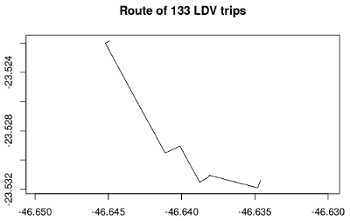
\includegraphics[width=4.86in]{figuras/gway} \caption{Driving route between zones 'Luz' and 'Bom Retiro' in São Paulo}\label{fig:unnamed-chunk-37}
\end{figure}

\subsubsection{The R package dodgr}\label{the-r-package-dodgr}

dpdgr\citep{dodgr} is a new R package with excellent capabilities. It
calculates the distance on dual-weight graphs using priority-queue
shortest paths. To calculate the traffic flows it is necessary to have
the matrix OD for the desired mode of transport and the coordinates of
centroids of the OD zones.

The function \texttt{dodgr\_streetnet} uses the osmdata R package to
download street network data from Open Street Map \citep{osm} for the
points of the centroids of zones OD. Depending on the spatial extent of
the data, the resulting data can be large. The function
\texttt{weight\_streetnet} weight the lines from OSM road network
according to a specific profile of traffic: ``psv'' for Public Service
Vehicle. ``bicycle'', and others. The weights are profile values for the
OSM type of roads based on this webpage:
\url{https://www.routino.org/xml/routino-profiles.xml}. The function
\texttt{dodgr\_vertices} extract the vertices of the graph including the
coordinates. Finally, the function \texttt{dodgr\_flowmap} reads the
graph and plots the flows. Below is an example for São Paulo using the
data of ODS \citep{ODS}.

\begin{figure}

{\centering 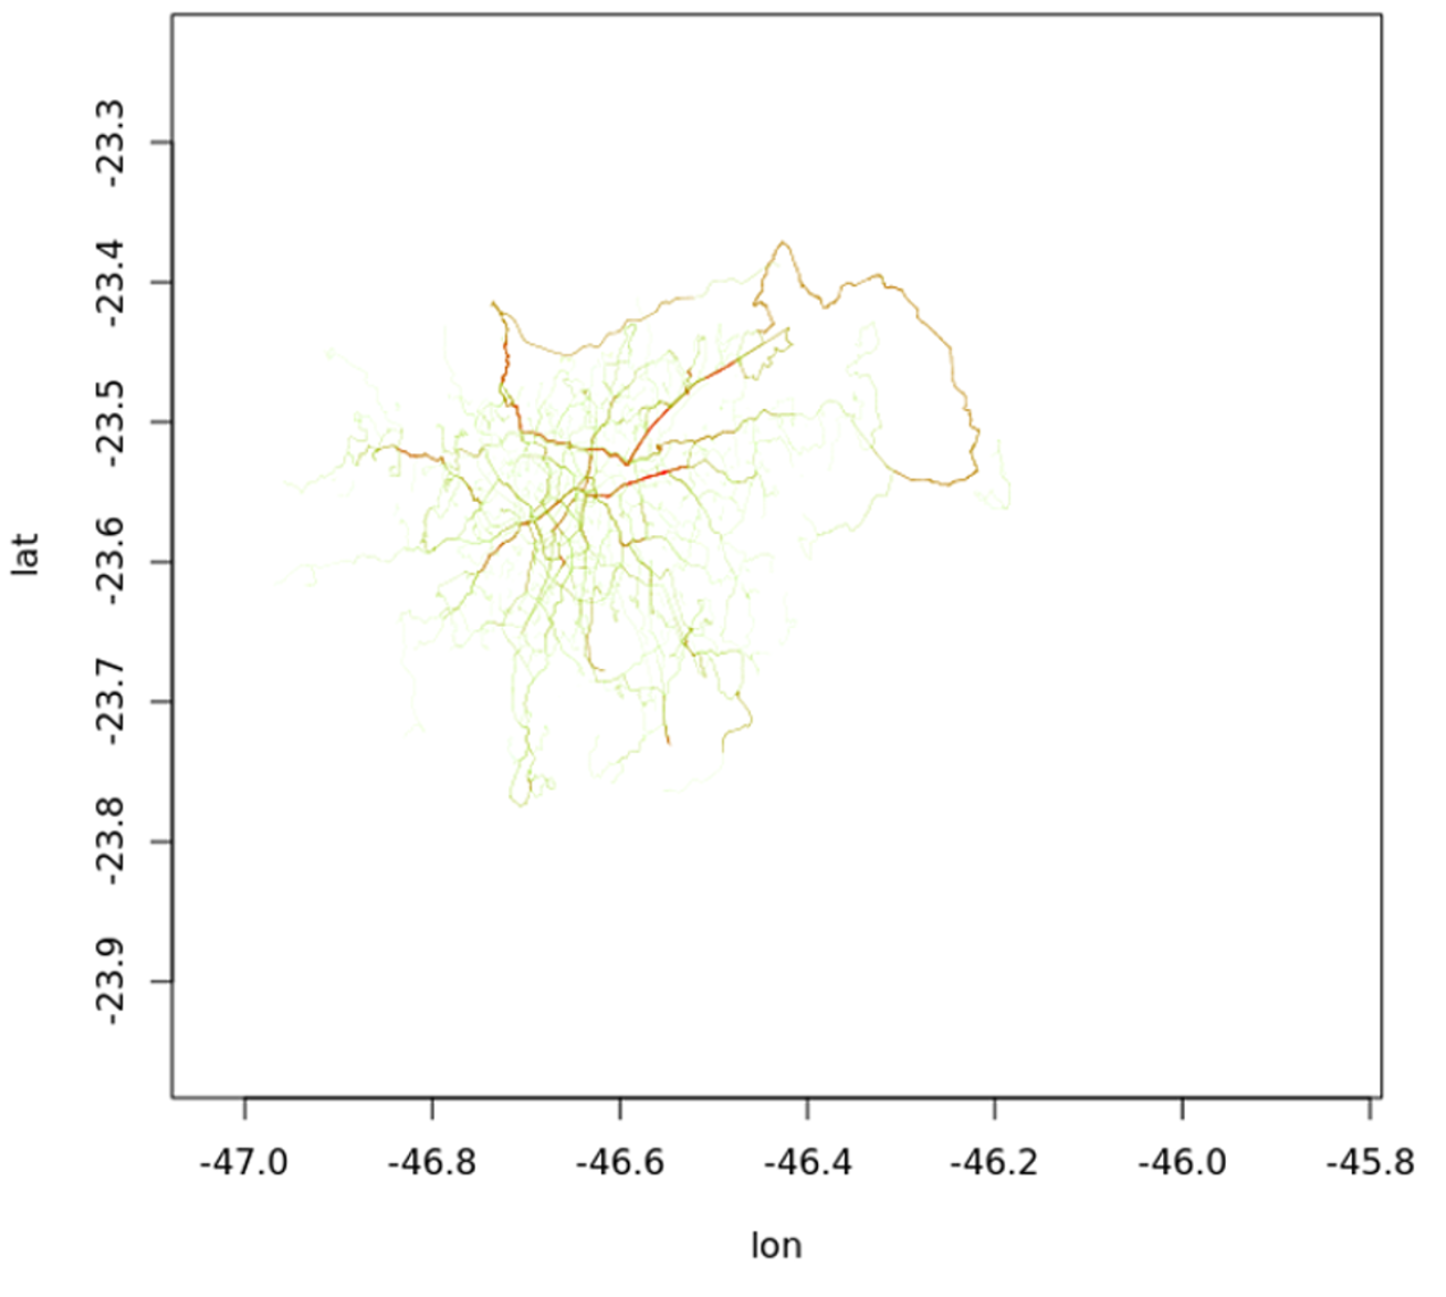
\includegraphics[width=4.82in]{figuras/dodgr} 

}

\caption{Daily trips of Light Duty Vehicles in São Paulo}\label{fig:rdodgr}
\end{figure}

\subsection{Top-down approach}\label{top-down-approach}

I designed VEIN with traffic flow at street level on the mind. However,
it is possible that the user might want or need to use a top-down
approach. Here are some possible causes:

\begin{enumerate}
\def\labelenumi{\arabic{enumi}.}
\tightlist
\item
  Bottom-up approach can demand more computational resources for a
  country or a continent.
\item
  Another possibility is that the emissions inventory is going to be
  used solely for air quality modeling purposes, where the proportion of
  grid spacing and the street is such that spatial detail would be
  loose, for instance with a resolution of 10 km.
\item
  Also, it is possible that there is no way of obtaining traffic
  information at street level.
\item
  Limited resources, time, funding, human resources.
\item
  Lastly, due to simplism. It is also possible that the objective is to
  estimate an emissions inventory using a top-down approach.
\end{enumerate}

Under these circumstances, a top-down approach would be better suited
for some users. As VEIN is a toolkit for estimating emissions, it is
reasonable to use all VEIN resources with a top-down approach.

In this case, the user must follow some considerations:

\begin{itemize}
\tightlist
\item
  Use \texttt{inventory} functions in the same way as shown in section
  \ref{st}.
\item
  Create a network, but instead of using a road network with spatial
  lines, use spatial polygons. The Spatial polygon might represent some
  area where the amount of vehicles is known.
\item
  The \texttt{age} functions shown in the following sections show that
  it is possible to apply age distributions to each street, in this
  case, to each area.
\end{itemize}

The Fig. \ref{fig:ftd} showed the emissions of PM for each state Brazil
and prepared for a congress using VEIN as a top-down tool
\citep{ibarraigac}.

\begin{figure}
\centering
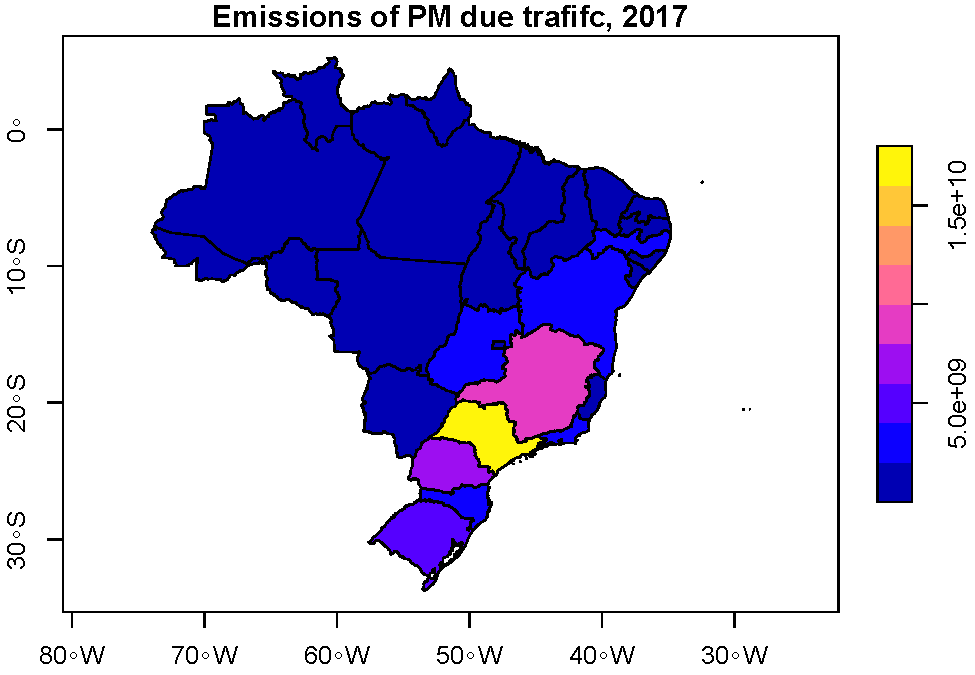
\includegraphics{veinbook_files/figure-latex/ftd-1.pdf}
\caption{\label{fig:ftd}Emissions of PM due trafifc, 2017}
\end{figure}

\section{Main functions}\label{main-functions}

The Fig.(\ref{fig:diavein}) shows a complete diagram with the steps for
elaborating an emissions inventory. Also, the function
\texttt{inventory} shown on sub-section (\ref{veinstructure}) shows the
functions to structure an inventory. The following subsection shows the
part of the diagram Fig.(\ref{fig:diatraffic}) and how to run VEIN as
well as storing the results in the directories shown in Fig. (\ref{st}).

The first element that the user must have is the traffic at street
level, shown as a green circle with the word `traffic' in Fig.
(\ref{fig:diatraffic}). The user must use any \texttt{age} function
which produces objects of class \texttt{Vehicles}. The function
\texttt{netspeed} produces an object of class \texttt{Speed}. The
\texttt{emis} function requires this objects.

\begin{figure}

{\centering 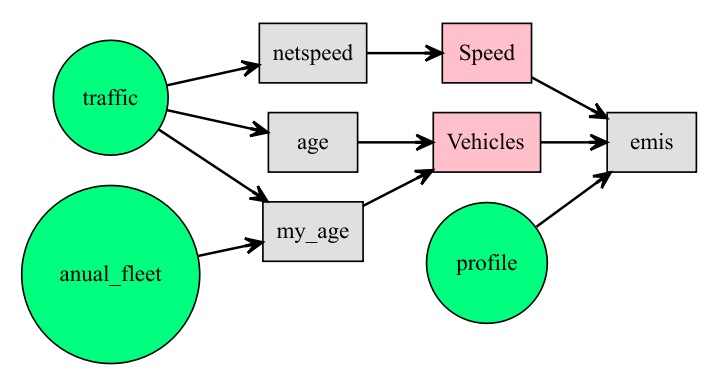
\includegraphics[width=1\linewidth]{figuras/dia4} 

}

\caption{Structuring an emissions inventories with VEIN}\label{fig:diatraffic}
\end{figure}

\subsection{\texorpdfstring{Expanding traffic data with the function
\texttt{temp\_fact}}{Expanding traffic data with the function temp\_fact}}\label{expanding-traffic-data-with-the-function-temp_fact}

Traffic data must be temporally extrapolated because it is usually
available only for the morning rush hour. Traffic data can be estimated
from short period traffic count datasets, then expanded to represent
longer timespan, such as Annual Average Daily Traffic (AADT;
\citep[lam2000estimation]{wang2009forecasting}). The next step is to
extrapolate the vehicular flow at street link \(i\), vehicle type \(j\),
and age of use \(k\), to obtain the vehicular flow for the hour of the
week \(l\) (\(F_{i,j,k,l}\); see equation \eqref{eq:flowx}.

\begin{equation}
F_{i,j,k,l} = F^*_{i,j,k} \cdot TF_{j,l}
\label{eq:flowx}
\end{equation}

Where \(TF_{j,l}\) are the temporal factors varying according to each
hour of \(l\) and type of vehicle \(j\). For instance, \(TF\) is defined
as a matrix with 24 lines and numbers of columns to each day considered,
from Monday to Sunday. \(TF\) matrices must be normalized to the hour
that represents the traffic data. It means that \(TF\) values at morning
peak hour must be 1 and the respective proportion are assigned to the
other hours. For example, \(TF\) values are obtained from automatic
traffic count stations.

The function \texttt{temp\_fact} return \(F_{i,j,k,l}\) as an object
with class \texttt{Vehicles}. The arguments are:

\begin{itemize}
\tightlist
\item
  \texttt{q} is a data-frame of traffic flow to each hour (veh/h) at
  each street.
\item
  \texttt{pro} s a matrix or data-frame to extrapolate.
\end{itemize}

\subsection{\texorpdfstring{Calculating speed at other hours with the
function
\texttt{netspeed}}{Calculating speed at other hours with the function netspeed}}\label{calculating-speed-at-other-hours-with-the-function-netspeed}

The average speed of traffic flow is critical, and it must be determined
for each link an hour. Once the vehicular flow is identified for each
hour, the average speed is then identified for each hour, using the
curves from the Bureau of Public Roads (BPR; \citep{bpr}), as shown in
Eq. \eqref{eq:bpr}. The process involves calculating speed by dividing the
length of the road by the time. The time is calculated using the total
traffic expanded to each street link \(i\) and hour \(l\).

\begin{equation}
T_{i,l} = To_i \cdot \left(1 +\alpha \cdot \left(\dfrac{Q_{i,l}}{C_i}\right)^\beta \right)
\label{eq:bpr}
\end{equation}

The function \texttt{netspeed} do these calculations. The arguments of
this function are:

\begin{Shaded}
\begin{Highlighting}[]
\KeywordTok{args}\NormalTok{(netspeed)}
\end{Highlighting}
\end{Shaded}

\begin{verbatim}
## function (q = 1, ps, ffs, cap, lkm, alpha = 0.15, beta = 4, net, 
##     scheme = FALSE, distance = "km", time = "h", isList) 
## NULL
\end{verbatim}

\texttt{netspeed} allows creates two types of speeds data-frames which
depends on the availability of data by the user. If the user has
\texttt{q}, \texttt{ps}, \texttt{ffs} and \texttt{cap} the user can use
the argument \texttt{scheme\ =\ FALSE}, or when the user only has
\texttt{ps} and \texttt{ffs} the user can use the argument
\texttt{scheme\ =\ TRUE}.

\begin{itemize}
\tightlist
\item
  \texttt{q} is a data-frame of traffic flow to each hour (veh/h) at
  each street.
\item
  \texttt{ps}is the Peak speed (km/h) at each street.
\item
  \texttt{ffs} Free flow speed (km/h) at each street.
\item
  \texttt{cap} Capacity of the link (veh/h) at each street.
\item
  \texttt{lkm} Distance of link (km) of each street.
\item
  \texttt{alpha} Parameter of \citet{bpr} curves.
\item
  \texttt{beta} Parameter of \citet{bpr} curves.
\item
  \texttt{scheme} Logical to create a Speed data-frame with 24 hours and
  a default profile. It needs \texttt{ffs} and \texttt{ps} at each
  street:
\end{itemize}

\begin{table}

\caption{\label{tab:unnamed-chunk-40}speeds for scheme = T}
\centering
\begin{tabular}[t]{cc}
\toprule
Period & Speed\\
\midrule
00:00-06:00 & ffs (Free flow speed)\\
06:00-07:00 & average between ffs and ps\\
07:00-10:00 & ps (Peakspeed)\\
10:00-17:00 & average between ffs and ps\\
17:00-20:00 & ps (Peak speed)\\
\addlinespace
20:00-22:00 & average between ffs and ps\\
22:00-00:00 & ffs (Free flow speed)\\
\bottomrule
\end{tabular}
\end{table}

\subsection{\texorpdfstring{Distribution of vehicles by age of use with
the functions \texttt{age\_ldv}, \texttt{age\_hdv} and
\texttt{age\_moto}}{Distribution of vehicles by age of use with the functions age\_ldv, age\_hdv and age\_moto}}\label{distribution-of-vehicles-by-age-of-use-with-the-functions-age_ldv-age_hdv-and-age_moto}

These functions read traffic data at each street and return an object of
class \texttt{Vehicles}, which is a data-frame with the number of
vehicles at each street, and the number of columns represents the number
of vehicles at each age. The functions \texttt{age\_moto} and
\texttt{age\_hdv} are identical. These functions apply survival
equations into the fleet from \citet{MMA2011}. The arguments are:

\begin{itemize}
\tightlist
\item
  \texttt{x} numeric vector of vehicles at each street.
\item
  \texttt{name} word of the vehicle assigned to columns of dataframe.
\item
  \texttt{a} parameter of survival equation. The default value for
  \texttt{age\_ldv} is 1.698 and for \texttt{age\_hdv} and
  \texttt{age\_moto} is 0.2.
\item
  \texttt{b} parameter of survival equation. The default value for
  \texttt{age\_ldv} is -0.2 and for \texttt{age\_hdv} and
  \texttt{age\_moto} is 17.
\item
  \texttt{agemin} age of newest vehicles for that category. The default
  value is 1; however, it can be bigger than one when it is a vehicle
  that is not circulating more than a year ago.
\item
  \texttt{agemax} age of oldest vehicles for that category. The default
  value is 50, assuming that the oldest vehicle in circulation has 50
  years of use.
\item
  \texttt{k} multiplication factor. This factor helps to split the
  traffic \texttt{x} in the composition.
\item
  \texttt{bystreet} when TRUE it is expecting that \texttt{a} and
  \texttt{b} are numeric vectors with length equal to \texttt{x}. In
  other words, the values of \texttt{a} and \texttt{b} vary in each
  street.
\item
  \texttt{message} message with average age and the total number of
  vehicles.
\end{itemize}

\subsection{\texorpdfstring{The function
\texttt{my\_age}}{The function my\_age}}\label{the-function-my_age}

These functions also read traffic data at each street and return an
object of class \texttt{Vehicles}, which is a data-frame with the number
of vehicles at each street, and the columns represent the number of
vehicles at each age. However, it is based on data the user has and not
by parameters. Therefore, using this function with own data should
produce more representative results. The arguments are:

\begin{Shaded}
\begin{Highlighting}[]
\KeywordTok{args}\NormalTok{(my_age)}
\end{Highlighting}
\end{Shaded}

\begin{verbatim}
## function (x, y, name = "age", k = 1, pro_street, net, message = TRUE) 
## NULL
\end{verbatim}

\begin{itemize}
\tightlist
\item
  \texttt{x} numerical vector of vehicles at each street.
\item
  \texttt{y} Age distribution of vehicles. This parameter can be annual
  sales or annual registry for the category of vehicle.
\item
  \texttt{name} of the vehicle assigned to columns of dataframe.
\item
  \texttt{k} multiplication factor. This factor helps to split the
  traffic \texttt{x} in the composition.
\item
  \texttt{message} message with average age and the total number of
  vehicles.
\end{itemize}

\subsection{\texorpdfstring{The class
\texttt{Vehicles}}{The class Vehicles}}\label{the-class-vehicles}

\texttt{Vehicles} is a class in VEIN, shown in Fig.
(\ref{fig:diatraffic}). This class includes the methods \texttt{print},
\texttt{plot} and \texttt{summary}, meaning that, \texttt{Vehicles}
objects presents customized versions of \texttt{print}, \texttt{plot}
and \texttt{summary} to make easier to the user to use VEIN. The figure
@ref(fig.plotpc) shows a simple plot of a \texttt{Vehicles} object,
followed by the \texttt{head} of this object. The plot shows the sum of
each type of vehicle by the age of use, with a vertical red line
indicating the average age, 11.17 years of use.

\begin{Shaded}
\begin{Highlighting}[]
\KeywordTok{library}\NormalTok{(vein)}
\KeywordTok{data}\NormalTok{(net)}
\NormalTok{PC_E25 <-}\StringTok{ }\KeywordTok{age_ldv}\NormalTok{(}\DataTypeTok{x =}\NormalTok{ net}\OperatorTok{$}\NormalTok{ldv,}\DataTypeTok{name =} \StringTok{"PC_E25"}\NormalTok{, }\DataTypeTok{k =} \DecValTok{75}\OperatorTok{/}\DecValTok{100}\OperatorTok{*}\FloatTok{37.25}\NormalTok{, }\DataTypeTok{message =}\NormalTok{ F)}
\KeywordTok{plot}\NormalTok{(PC_E25)}
\end{Highlighting}
\end{Shaded}

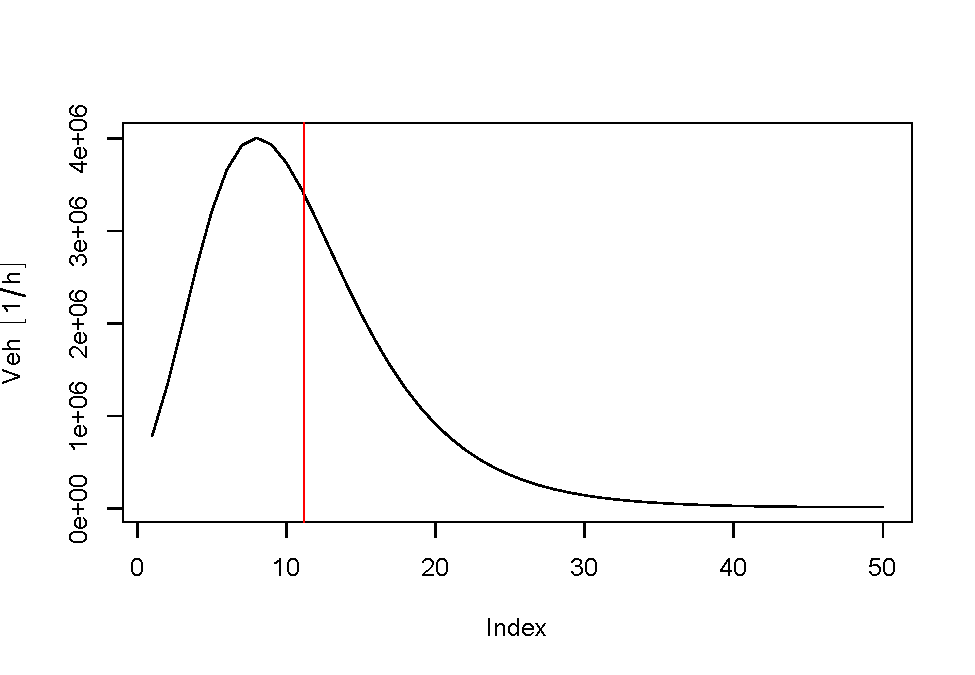
\includegraphics{veinbook_files/figure-latex/plotpc-1.pdf}

\begin{verbatim}
## 
## Average =  11.17
\end{verbatim}

\begin{Shaded}
\begin{Highlighting}[]
\KeywordTok{head}\NormalTok{(PC_E25[, }\DecValTok{1}\OperatorTok{:}\DecValTok{4}\NormalTok{]) }\CommentTok{# The first 4 columns}
\end{Highlighting}
\end{Shaded}

\begin{verbatim}
## Result for Vehicles 
##                 V1               V2               V3               V4
## 1 1761.92888 [1/h] 2968.78285 [1/h] 4404.60761 [1/h] 5877.97812 [1/h]
## 2  591.76508 [1/h]  997.10155 [1/h] 1479.34063 [1/h] 1974.18989 [1/h]
## 3  240.18939 [1/h]  404.70994 [1/h]  600.44421 [1/h]  801.29679 [1/h]
## 4  341.44967 [1/h]  575.32964 [1/h]  853.58258 [1/h] 1139.11162 [1/h]
## 5   22.27726 [1/h]   37.53633 [1/h]   55.69044 [1/h]   74.31926 [1/h]
## 6 1163.27810 [1/h] 1960.07916 [1/h] 2908.05358 [1/h] 3880.81682 [1/h]
\end{verbatim}

\subsection{Other traffic functions}\label{other-traffic-functions}

Another function is \texttt{adt} which calculates average daily traffic
(ADT) from Hourly traffic data. This function reads numeric vectors with
the number of vehicles at each street and expands the traffic with
temporal factors for each type of vehicle. The arguments are:

\begin{Shaded}
\begin{Highlighting}[]
\KeywordTok{args}\NormalTok{(adt)}
\end{Highlighting}
\end{Shaded}

\begin{verbatim}
## function (pc, lcv, hgv, bus, mc, p_pc, p_lcv, p_hgv, p_bus, p_mc, 
##     expanded = FALSE) 
## NULL
\end{verbatim}

\begin{itemize}
\tightlist
\item
  \texttt{pc} numeric vector for passenger cars
\item
  \texttt{lcv} numeric vector for light commercial vehicles
\item
  \texttt{hgv} numeric vector for heavy good vehicles or trucks
\item
  \texttt{bus} numeric vector for bus
\item
  \texttt{mc} numeric vector for motorcycles
\item
  \texttt{p\_pc} data-frame profile for passenger cars
\item
  \texttt{p\_lcv} data-frame profile for light commercial vehicles
\item
  \texttt{p\_hgv} data-frame profile for heavy good vehicles or trucks
\item
  \texttt{p\_bus} data-frame profile for bus
\item
  \texttt{p\_mc} data-frame profile for motorcycles
\end{itemize}

\section{Vehicular composition}\label{vehicular-composition}

\section{Application}\label{application}

As mentioned above, the application consists of using the travel demand
model for the west part of São Paulo city, present in VEIN. This script
reads traffic data and expands it applying an age function. It uses the
\texttt{inventory} function with the default vehicular composition,
shown in section (@red(st)).

\begin{Shaded}
\begin{Highlighting}[]
\KeywordTok{library}\NormalTok{(vein)}
\KeywordTok{inventory}\NormalTok{(}\KeywordTok{file.path}\NormalTok{(}\KeywordTok{tempdir}\NormalTok{(), }\StringTok{"YourCity"}\NormalTok{))}
\KeywordTok{setwd}\NormalTok{(}\StringTok{"YourCity"}\NormalTok{)}
\KeywordTok{data}\NormalTok{(net) }\CommentTok{# Loads the traffic demand simulation for west São Paulo}
\KeywordTok{data}\NormalTok{(net)}
\KeywordTok{data}\NormalTok{(pc_profile)}
\NormalTok{pc_week <-}\StringTok{ }\KeywordTok{temp_fact}\NormalTok{(net}\OperatorTok{$}\NormalTok{ldv}\OperatorTok{+}\NormalTok{net}\OperatorTok{$}\NormalTok{hdv, pc_profile)}
\NormalTok{speed <-}\StringTok{ }\KeywordTok{netspeed}\NormalTok{(pc_week, net}\OperatorTok{$}\NormalTok{ps, net}\OperatorTok{$}\NormalTok{ffs, net}\OperatorTok{$}\NormalTok{capacity, net}\OperatorTok{$}\NormalTok{lkm)}
\KeywordTok{saveRDS}\NormalTok{(net, }\DataTypeTok{file =} \StringTok{"network/net.rds"}\NormalTok{)}
\KeywordTok{saveRDS}\NormalTok{(speed, }\DataTypeTok{file =} \StringTok{"network/speed.rds"}\NormalTok{)}
\end{Highlighting}
\end{Shaded}

\chapter{Emission Factors}\label{ef}

An emission factor is the amount of mass of pollutant generated by
activities \citep{pulles2010art}. In the case of vehicles, the emission
factor is the mass of pollutant per traveled distance
\(g \cdot km^{-1}\) in metric units. The distance unit could be
different, like miles for instance. The type of groups depends on the
measurement used when developing the emission factors.

There are hot and cold exhaust emissions. \emph{Hot} exhaust emissions
are produced by a vehicle when its engine and exhaust after-treatment
system are at their normal operating temperatures and \emph{Cold} during
the vehicle warm-up phase \citep{trlef}.

The emission factors come from measurements of pollutants emitted by the
sources. In the case of vehicles, the dynamometer measurements of the
emission factors are the mass of pollutant collected during the distance
traveled by a vehicle following a specific driving cycle. The Federal
Test Procedure (FTP) is a test to certify the vehicle emissions under
the driving cycles such as FTP-75. This driving cycle has a duration of
1874 \(s\) for a distance of 17783 \(m\) and an average speed of 34.12
\(km \cdot h^{-1}\) \citep{tim}.

In the literature, it is possible to find the different type of emission
factors. For instance, in Europe, during the development of the project
Assesment of Reliability of Transport Emission Models and Inventory
Systems (ARTEMIS), the \emph{traffic situation model} was developed. The
model concept consists in the combination of parameters that affects
vehicle kinematics and engine operation: type of road, sinuosity and
gradient, traffic conditions or level of service (free-flow, heavy,
saturated and stop and go) and average speed by the speed limit of the
road \citep{artemis}. Measurements of vehicular emissions under each
traffic situation lead to emission factors by traffic situation, used in
the Handbook of Emission Factors (HBEFA, www.hbefa.net).

There is another approach based on a 1 Hz measurement of emissions,
where the pollutants are measured on real live traffic driving. Emission
factors can be derived here using mainly two approaches. One approach is
applying the Vehicular Specific Power (VSP) \citep{jimenez1999vehicle}.
This method is used in the Motor Vehicle Emission Simulator (MOVES)
\citep{koupal2003design} and the International Vehicle Emissions model
(IVE) \citep{Davisetal2005}. Another approach is to apply the Passenger
car, and Heavy-duty Emission Model (PHEM), which is based on
instantaneous engine power demand and engine speed developed during the
ARTEMIS project \citep[\citet{artemis}]{tim}.

Perhaps the most used approach to obtain emission factors are speed
functions. As emissions tests on driving cycles are valid for only one
average speed, measuring emissions of different driving cycles at
different average speeds, allows obtaining point clouds where regression
is applied, obtaining an emission factor as a speed function. The
literature shows experiments in different parts of the world, such as in
Chile \citep{Corvalanetal2002} and Europe
\citep{ntziachristos2000speed}. However, probably the most used source
of emission factors as speed functions are the European emission
guidelines developed by the European Monitoring and Evaluation Programme
(EMEP, \url{http://www.emep.int/}) and published by the European
Environment Agency (EEA,
\url{https://www.eea.europa.eu/themes/air/emep-eea-air-pollutant-emission-inventory-guidebook/emep})
\citep{NtziachristosSamaras2016}. These emission factors are included in
the VEIN model.

Another aspect important in vehicular emissions is the degradation of
the emissions of old vehicles. Over time, the different part of the cars
suffers deterioration, increasing the emissions. Therefore, approaches
have been developed to account for this effect in inventories. One
method consists in determining functions that increment the emissions by
accumulated mileage, such as studies of \citet{CorvalanVargas2003}.

In Brazil, the emission factors are reported by the Environmental
Protection Agency of São Paulo \citet{CETESB2015}, in their vehicular
emissions inventory report. Light vehicles emission factors come from
average measurements of the FTP75 driving cycle, and motorcycle emission
factors come from average measurements of World Motorcycle Test Cycle
(WMTC) and HDV from the European Stationary Cycle (ETC).

I developed the VEIN model in Brazil, but users of other parts of the
world may be interested in using the model, the approach in VEIN has to
allow flexibility to the user. Therefore, the emission factors approach
in VEIN consists of three options, as shown in Fig. (\ref{fig:diaef}).
The first approach consists of local emissions factors by the age of
use, such as the one from \citet{CETESB2015}, denoted as local\_ef in
the green circle. The second approach consisted in selecting speed
functions from \citet{NtziachristosSamaras2016}, available in VEIN and
denoted as the grey box as speed\_ef. The third approach consists in
incorporating speed variation from the speed function into the local
emission factors by the age of use. In any case, VEIN uses a function to
account for the degradation of emissions due to accumulated mileage
(denoted in a grey box as emis\_det). These emissions are inputted into
the emission estimation function.

The following sections show how to do this calculation in VEIN, step by
step.

\begin{figure}

{\centering 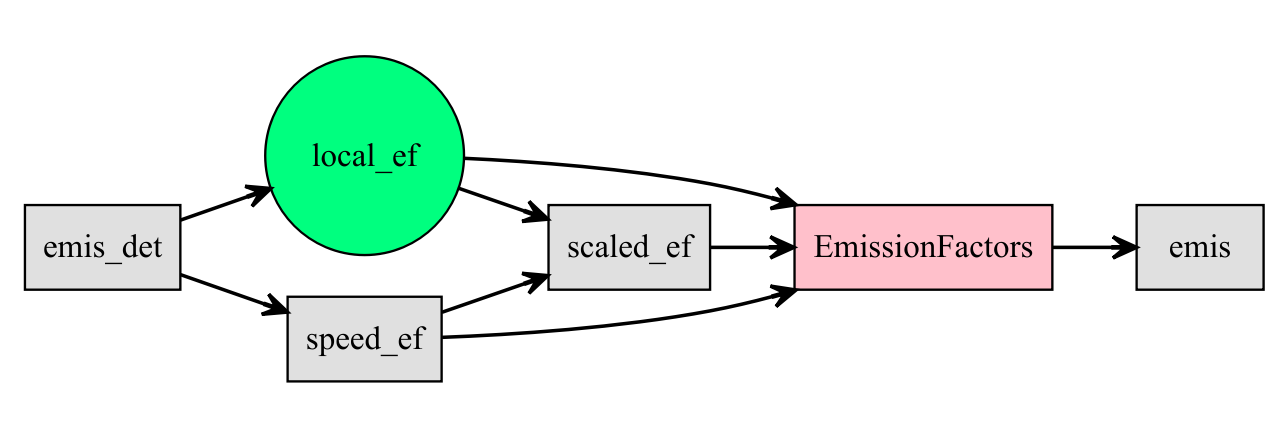
\includegraphics[width=1\linewidth]{figuras/dia5} 

}

\caption{Structuring an emissions inventories with VEIN}\label{fig:diaef}
\end{figure}

\section{\texorpdfstring{Speed functions \texttt{ef\_ldv\_speed} and
\texttt{ef\_hdv\_speed}}{Speed functions ef\_ldv\_speed and ef\_hdv\_speed}}\label{speedef}

The estimation of emissions in VEIn is shown the equation \eqref{eq:emi}:

\begin{equation}
EH_{i,j,k,l,m} =F_{i,j,k,l} \cdot L_i \cdot EF(V_{i,l})_{j,k,m} \cdot DF_{j,k}
\label{eq:emi}
\end{equation}

where \(EH_{i,j,k,l,m}\) is the emission for each street link \(i\),
vehicle category from composition \(k\), hour \(l\) and pollutant \(m\),
\(F_{i,j,k,l}\) is the vehicular flow calculated in Eq. 1. \(L_i\) is
the length of the street link \(i\). \(EF(V_{i,l})_{j,k,m}\) is the
emission factor of each pollutant \(m\). \(DF_{j,k}\) is the
deterioration factor for vehicle of type \(j\) and age of use \(k\),
explained in detail in section \ref{det}.

These functions return speed functions as \(f(V)\). The functions come
from the EMEP/EEA emissions guidelines \citep{NtziachristosSamaras2016}
and are available in PDF reports. The equations and their parameters
were translated to a spreadsheet and loaded internally in VEIN.
Therefore, the user only must enter the required parameters obtaining
the desired function. The functions respect the assumptions and speed
limits.

\subsection{\texorpdfstring{Emission factors of LDV depending on the
speed with the function
\texttt{ef\_ldv\_speed}}{Emission factors of LDV depending on the speed with the function ef\_ldv\_speed}}\label{emission-factors-of-ldv-depending-on-the-speed-with-the-function-ef_ldv_speed}

The arguments for \texttt{ef\_ldv\_speed} are:

\begin{itemize}
\tightlist
\item
  \texttt{v}: Category of vehicle: ``PC'', ``LCV'', ``Motorcycle'' or
  ``Moped''.
\item
  \texttt{t}: Sub-category of vehicle: PC: ``ECE\_1501'', ``ECE\_1502'',
  ``ECE\_1503'', ``ECE\_1504'' , ``IMPROVED\_CONVENTIONAL'',
  ``OPEN\_LOOP'', ``ALL'', ``2S'' or ``4S''. LCV: ``4S'', Motorcycle:
  ``2S'' or ``4S''. Moped: ``2S'' or ``4S''.
\item
  \texttt{cc}: Size of engine in cc: PC: ``\textless{}=1400'',
  ``\textgreater{}1400'', ``1400\_2000'', ``\textgreater{}2000'',
  ``\textless{}=800'', ``\textless{}=2000''. Motorcycle:
  ``\textgreater{}=50'' (for ``2S''), ``\textless{}=250'', ``250\_750'',
  ``\textgreater{}=750''. Moped: ``\textless{}=50''. LCV :
  ``\textless{}3.5'' for gross weight.
\item
  \texttt{f}: Type of fuel: ``G'', ``D'', ``LPG'' or ``FH'' (Full
  Hybrid: starts by electric motor).
\item
  \texttt{eu}: Euro standard: ``PRE'', ``I'', ``II'', ``III'',
  ``III+DPF'', ``IV'', ``V'', ``VI'' or ``VIc''.
\item
  \texttt{p}: Pollutants: \textbf{Criteria}: ``CO'', ``NOx'', ``HC'',
  ``PM'', ``CH4'', ``NMHC'', ``CO2'', ``SO2'', ``Pb'', ``FC'' (Fuel
  Consumption).
\item
  \textbf{PAH and POP}: ``indeno(1,2,3-cd)pyrene'',
  ``benzo(k)fluoranthene'', ``benzo(b)fluoranthene'',
  ``benzo(ghi)perylene'', ``fluoranthene'', ``benzo(a)pyrene'',
  ``pyrene'', ``perylene'', ``anthanthrene'', ``benzo(b)fluorene'',
  ``benzo(e)pyrene'', ``triphenylene'', ``benzo(j)fluoranthene'',
  ``dibenzo(a,j)anthacene'', ``dibenzo(a,l)pyrene'',
  ``3,6-dimethyl-phenanthrene'', ``benzo(a)anthracene'',
  ``acenaphthylene'', ``acenapthene'', ``fluorene'', ``chrysene'',
  ``phenanthrene'', ``napthalene'', ``anthracene'', ``coronene'',
  ``dibenzo(ah)anthracene'' \textbf{Dioxins and Furans}: ``PCDD'',
  ``PCDF'', ``PCB''.
\item
  \textbf{Metals}: ``As'', ``Cd'', ``Cr'', ``Cu'', ``Hg'', ``Ni'',
  ``Pb'', ``Se'', ``Zn''.
\item
  \textbf{NMHC}:
\item
  \emph{ALKANES}: ``ethane'', ``propane'', ``butane'', ``isobutane'',
  ``pentane'', ``isopentane'', ``hexane'', ``heptane'', ``octane'',
  ``TWO\_methylhexane'', ``nonane'', ``TWO\_methylheptane'',
  ``THREE\_methylhexane'', ``decane'', ``THREE\_methylheptane'',
  ``alcanes\_C10\_C12'', ``alkanes\_C13''.
\item
  \emph{CYCLOALKANES}: ``cycloalcanes''.
\item
  \emph{ALKENES}: ``ethylene'', ``propylene'', ``propadiene'',
  ``ONE\_butene'', ``isobutene'', ``TWO\_butene'',
  ``ONE\_3\_butadiene'', ``ONE\_pentene'', ``TWO\_pentene'',
  ``ONE\_hexene'', ``dimethylhexene''.
\item
  \emph{ALKYNES}:``ONE\_butine'', ``propine'', ``acetylene''.
\item
  \emph{ALDEHYDES}: ``formaldehyde'', ``acetaldehyde'', ``acrolein'',
  ``benzaldehyde'', ``crotonaldehyde'', ``methacrolein'',
  ``butyraldehyde'', ``isobutanaldehyde'', ``propionaldehyde'',
  ``hexanal'', ``i\_valeraldehyde'', ``valeraldehyde'',
  ``o\_tolualdehyde'', ``m\_tolualdehyde'', ``p\_tolualdehyde''.
\item
  KETONES: ``acetone'', ``methylethlketone''.
\item
  \emph{AROMATICS}: ``toluene'', ``ethylbenzene'', ``m\_p\_xylene'',
  ``o\_xylene'', ``ONE\_2\_3\_trimethylbenzene'',
  ``ONE\_2\_4\_trimethylbenzene'', ``ONE\_3\_5\_trimethylbenzene'',
  ``styrene'', ``benzene'', ``C9'', ``C10'', ``C13''.
\item
  \texttt{k}: Multiplication factor.
\item
  \texttt{show.equation}: Option to see (or not) the equation
  parameters.
\end{itemize}

It is essential that the user enters the right values into the arguments
because the final category must match. If the user enters values that do
not match, the resulting speed function will be wrong. There are 146
matches. The probably most used combinations are:

\begin{table}

\caption{\label{tab:unnamed-chunk-45}Most used combinations for emission factors for LDV}
\centering
\begin{tabular}[t]{ll}
\toprule
Argument & Value\\
\midrule
v & PC LCV Motorcycles\\
t & 4S\\
cc & <=1400 1400\_2000 >2000\\
f & G D\\
eu & PRE I II III IV V VI\\
p & CO NOx HC FC PM\\
\bottomrule
\end{tabular}
\end{table}

The returning speed function represents how a type of vehicle emits
pollutants on average. The Fig. (\ref{fig:figef}) shows the emissions of
CO by Passenger Cars with technologies Pre Euro and Euro I from
\citet{NtziachristosSamaras2016}. Higher emissions occurs at low average
speeds and older vehicles with technologies pre Euro emit more than
vehicles with Euro I. Even more, the average emissions of Pre Euro are
29.31 \(g \cdot km^{-1}\) and Euro I 2.61 \(g \cdot km^{-1}\), meaning
that, on average, a vehicle Pre euro is 14 times higher than a vehicle
with euro I.

The Fig. (\ref{fig:figef}) shows the plot using the package ggplot2
\citep{ggplot2}. This package requires that the data must be in long
format.

\begin{Shaded}
\begin{Highlighting}[]
\KeywordTok{library}\NormalTok{(vein)}
\KeywordTok{library}\NormalTok{(ggplot2)}
\NormalTok{ef1 <-}\StringTok{ }\KeywordTok{ef_ldv_speed}\NormalTok{(}\DataTypeTok{v =} \StringTok{"PC"}\NormalTok{, }\DataTypeTok{cc =} \StringTok{"<=1400"}\NormalTok{, }\DataTypeTok{f =} \StringTok{"G"}\NormalTok{,}
                    \DataTypeTok{eu =} \StringTok{"PRE"}\NormalTok{, }\DataTypeTok{p =} \StringTok{"CO"}\NormalTok{, }\DataTypeTok{show.equation =}\NormalTok{ F)}
\NormalTok{ef2 <-}\StringTok{ }\KeywordTok{ef_ldv_speed}\NormalTok{(}\DataTypeTok{v =} \StringTok{"PC"}\NormalTok{, }\DataTypeTok{cc =} \StringTok{"<=1400"}\NormalTok{, }\DataTypeTok{f =} \StringTok{"G"}\NormalTok{,}
                    \DataTypeTok{eu =} \StringTok{"I"}\NormalTok{, }\DataTypeTok{p =} \StringTok{"CO"}\NormalTok{, }\DataTypeTok{show.equation =}\NormalTok{ F)}
\NormalTok{V <-}\StringTok{ }\DecValTok{0}\OperatorTok{:}\DecValTok{110}
\NormalTok{df <-}\StringTok{ }\KeywordTok{data.frame}\NormalTok{(}\DataTypeTok{EF =} \KeywordTok{c}\NormalTok{(}\KeywordTok{ef1}\NormalTok{(V), }\KeywordTok{ef2}\NormalTok{(V)))}
\NormalTok{df}\OperatorTok{$}\NormalTok{V =}\StringTok{ }\NormalTok{V}
\NormalTok{df}\OperatorTok{$}\NormalTok{Euro <-}\StringTok{ }\KeywordTok{factor}\NormalTok{(}\KeywordTok{c}\NormalTok{(}\KeywordTok{rep}\NormalTok{(}\StringTok{"PRE"}\NormalTok{, }\DecValTok{111}\NormalTok{), }\KeywordTok{rep}\NormalTok{(}\StringTok{"I"}\NormalTok{, }\DecValTok{111}\NormalTok{)),}
                  \DataTypeTok{levels =} \KeywordTok{c}\NormalTok{(}\StringTok{"PRE"}\NormalTok{, }\StringTok{"I"}\NormalTok{))}
\KeywordTok{ggplot}\NormalTok{(df, }\KeywordTok{aes}\NormalTok{(V, EF, }\DataTypeTok{colour =}\NormalTok{ Euro)) }\OperatorTok{+}\StringTok{ }\KeywordTok{geom_point}\NormalTok{(}\DataTypeTok{size =} \DecValTok{3}\NormalTok{) }\OperatorTok{+}
\StringTok{  }\KeywordTok{geom_line}\NormalTok{() }\OperatorTok{+}\StringTok{ }\KeywordTok{theme_bw}\NormalTok{()}\OperatorTok{+}
\StringTok{  }\KeywordTok{labs}\NormalTok{(}\DataTypeTok{y =} \StringTok{"CO[g/km]"}\NormalTok{, }\DataTypeTok{x =} \StringTok{"[km/h]"}\NormalTok{)}
\end{Highlighting}
\end{Shaded}

\begin{figure}

{\centering 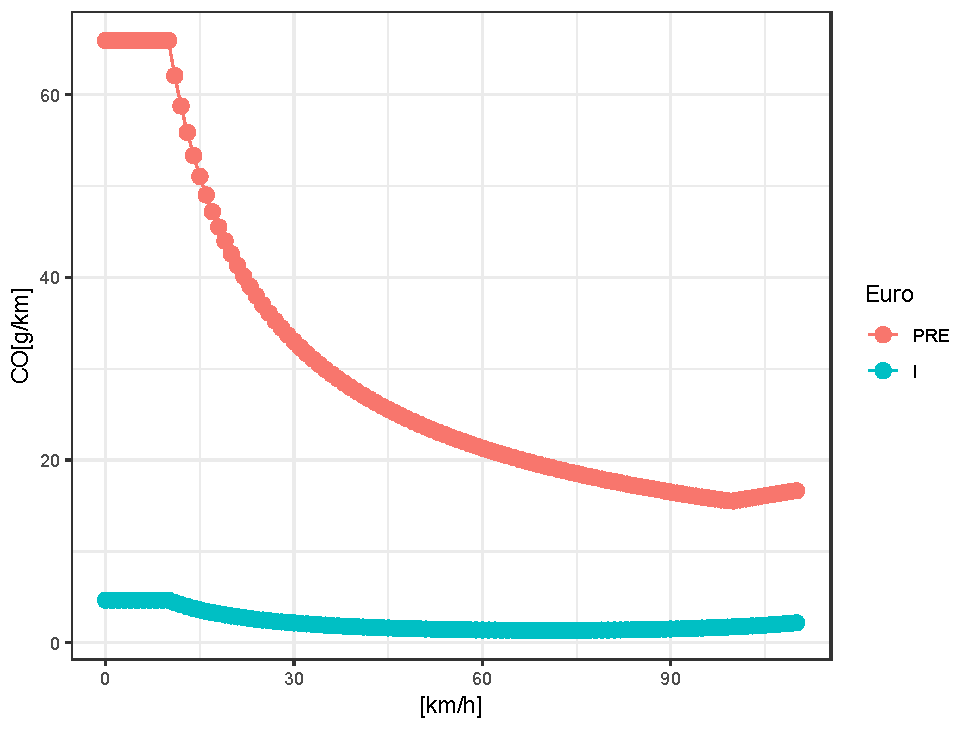
\includegraphics[width=0.8\linewidth]{veinbook_files/figure-latex/figef-1} 

}

\caption{Emission factor as a speed function}\label{fig:figef}
\end{figure}

\subsection{\texorpdfstring{Emission factors of HDV depending on the
speed with the function
\texttt{ef\_hdv\_speed}}{Emission factors of HDV depending on the speed with the function ef\_hdv\_speed}}\label{emission-factors-of-hdv-depending-on-the-speed-with-the-function-ef_hdv_speed}

The arguments for \texttt{ef\_hdv\_speed} are:

\begin{Shaded}
\begin{Highlighting}[]
\KeywordTok{args}\NormalTok{(ef_hdv_speed)}
\end{Highlighting}
\end{Shaded}

\begin{verbatim}
## function (v, t, g, eu, x, gr = 0, l = 0.5, p, k = 1, show.equation = FALSE) 
## NULL
\end{verbatim}

\begin{itemize}
\tightlist
\item
  \texttt{v} Category of vehicle: ``Coach'', ``Trucks'' or ``Ubus''
\item
  \texttt{t} Sub-category of vehicle: ``3Axes'', ``Artic'', ``Midi'',
  ``RT,''Std" and ``TT''
\item
  \texttt{g} Gross weight of each category: ``\textless{}=18'',
  ``\textgreater{}18'', ``\textless{}=15'', ``\textgreater{}15 \&
  \textless{}=18'', ``\textless{}=7.5'', - ``\textgreater{}7.5 \&
  \textless{}=12'', ``\textgreater{}12 \& \textless{}=14'',
  ``\textgreater{}14 \& \textless{}=20'', ``\textgreater{}20 \&
  \textless{}=26'', ``\textgreater{}26 \& \textless{}=28'',
  ``\textgreater{}28 \& \textless{}=32'', ``\textgreater{}32'',
  ``\textgreater{}20 \& \textless{}=28'', ``\textgreater{}28 \&
  \textless{}=34'', ``\textgreater{}34 \& \textless{}=40'',
  ``\textgreater{}40 \& \textless{}=50'' or ``\textgreater{}50 \&
  \textless{}=60''
\item
  `eu Euro emission standard: ``PRE'', ``I'', ``II'', ``III'', ``IV''
  and ``V''
\item
  `gr Gradient or slope of road: -0.06, -0.04, -0.02, 0.00, 0.02. 0.04
  or 0.06
\item
  \texttt{l} Load of the vehicle: 0.0, 0.5 or 1.0
\item
  \texttt{p} Pollutant: \textbf{Criteria}: ``CO'', ``NOx'', ``HC'',
  ``PM'', ``CH4'', ``NMHC'', ``CO2'', ``SO2'', ``Pb'', ``FC'' (Fuel
  Consumption).
\item
  \textbf{PAH and POP}: ``indeno(1,2,3-cd)pyrene'',
  ``benzo(k)fluoranthene'', ``benzo(b)fluoranthene'',
  ``benzo(ghi)perylene'', ``fluoranthene'', ``benzo(a)pyrene'',
  ``pyrene'', ``perylene'', ``anthanthrene'', ``benzo(b)fluorene'',
  ``benzo(e)pyrene'', ``triphenylene'', ``benzo(j)fluoranthene'',
  ``dibenzo(a,j)anthacene'', ``dibenzo(a,l)pyrene'',
  ``3,6-dimethyl-phenanthrene'', ``benzo(a)anthracene'',
  ``acenaphthylene'', ``acenapthene'', ``fluorene'', ``chrysene'',
  ``phenanthrene'', ``napthalene'', ``anthracene'', ``coronene'',
  ``dibenzo(ah)anthracene''
\item
  \textbf{Dioxins and Furans}: ``PCDD'', ``PCDF'', ``PCB''.
\item
  \textbf{Metals}: ``As'', ``Cd'', ``Cr'', ``Cu'', ``Hg'', ``Ni'',
  ``Pb'', ``Se'', ``Zn''.
\item
  \textbf{NMHC}:
\item
  \emph{ALKANES}: ``ethane'', ``propane'', ``butane'', ``isobutane'',
  ``pentane'', ``isopentane'', ``hexane'', ``heptane'', ``octane'',
  ``TWO\_methylhexane'', ``nonane'', ``TWO\_methylheptane'',
  ``THREE\_methylhexane'', ``decane'', ``THREE\_methylheptane'',
  ``alcanes\_C10\_C12'', ``alkanes\_C13''.
\item
  \emph{CYCLOALKANES}: ``cycloalcanes''.
\item
  \emph{ALKENES}: ``ethylene'', ``propylene'', ``propadiene'',
  ``ONE\_butene'', ``isobutene'', ``TWO\_butene'',
  ``ONE\_3\_butadiene'', ``ONE\_pentene'', ``TWO\_pentene'',
  ``ONE\_hexene'', ``dimethylhexene''.
\item
  \emph{ALKYNES}:``ONE\_butine'', ``propine'', ``acetylene''.
\item
  \emph{ALDEHYDES}: ``formaldehyde'', ``acetaldehyde'', ``acrolein'',
  ``benzaldehyde'', ``crotonaldehyde'', ``methacrolein'',
  ``butyraldehyde'', ``isobutanaldehyde'', ``propionaldehyde'',
  ``hexanal'', ``i\_valeraldehyde'', ``valeraldehyde'',
  ``o\_tolualdehyde'', ``m\_tolualdehyde'', ``p\_tolualdehyde''.
\item
  KETONES: ``acetone'', ``methylethlketone''.
\item
  \emph{AROMATICS}: ``toluene'', ``ethylbenzene'', ``m\_p\_xylene'',
  ``o\_xylene'', ``ONE\_2\_3\_trimethylbenzene'',
  ``ONE\_2\_4\_trimethylbenzene'', ``ONE\_3\_5\_trimethylbenzene'',
  ``styrene'', ``benzene'', ``C9'', ``C10'', ``C13''.
\item
  \texttt{k}: Multiplication factor.
\item
  \texttt{k} Multiplication factor
\item
  \texttt{show.equation} Option to see or not the equation parameters
\end{itemize}

\begin{Shaded}
\begin{Highlighting}[]
\NormalTok{V <-}\StringTok{ }\DecValTok{0}\OperatorTok{:}\DecValTok{130}
\NormalTok{ef1 <-}\StringTok{ }\KeywordTok{ef_hdv_speed}\NormalTok{(}\DataTypeTok{v =} \StringTok{"Trucks"}\NormalTok{,}\DataTypeTok{t =} \StringTok{"RT"}\NormalTok{, }\DataTypeTok{g =} \StringTok{"<=7.5"}\NormalTok{,}
                    \DataTypeTok{e =} \StringTok{"II"}\NormalTok{, }\DataTypeTok{gr =} \DecValTok{0}\NormalTok{,}
\DataTypeTok{l =} \FloatTok{0.5}\NormalTok{, }\DataTypeTok{p =} \StringTok{"HC"}\NormalTok{, }\DataTypeTok{show.equation =} \OtherTok{FALSE}\NormalTok{)}
\NormalTok{ef2 <-}\StringTok{ }\KeywordTok{ef_hdv_speed}\NormalTok{(}\DataTypeTok{v =} \StringTok{"Trucks"}\NormalTok{,}\DataTypeTok{t =} \StringTok{"RT"}\NormalTok{, }\DataTypeTok{g =} \StringTok{"<=7.5"}\NormalTok{,}
                    \DataTypeTok{e =} \StringTok{"II"}\NormalTok{, }\DataTypeTok{gr =} \FloatTok{0.06}\NormalTok{,}
\DataTypeTok{l =} \FloatTok{0.5}\NormalTok{, }\DataTypeTok{p =} \StringTok{"HC"}\NormalTok{, }\DataTypeTok{show.equation =} \OtherTok{FALSE}\NormalTok{)}
\KeywordTok{plot}\NormalTok{(}\DecValTok{1}\OperatorTok{:}\DecValTok{130}\NormalTok{, }\KeywordTok{ef1}\NormalTok{(}\DecValTok{1}\OperatorTok{:}\DecValTok{130}\NormalTok{), }\DataTypeTok{pch =} \DecValTok{16}\NormalTok{, }\DataTypeTok{type =} \StringTok{"b"}\NormalTok{,}
     \DataTypeTok{ylab =} \StringTok{"HC [g/km]"}\NormalTok{, }\DataTypeTok{xlab =} \StringTok{"Speed [km/h]"}\NormalTok{)}
\KeywordTok{lines}\NormalTok{(}\DecValTok{1}\OperatorTok{:}\DecValTok{130}\NormalTok{, }\KeywordTok{ef2}\NormalTok{(}\DecValTok{1}\OperatorTok{:}\DecValTok{130}\NormalTok{), }\DataTypeTok{pch =} \DecValTok{16}\NormalTok{, }\DataTypeTok{type =} \StringTok{"b"}\NormalTok{, }\DataTypeTok{col =} \StringTok{"blue"}\NormalTok{)}
\end{Highlighting}
\end{Shaded}

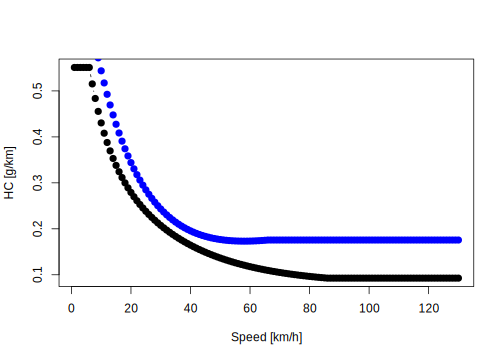
\includegraphics{veinbook_files/figure-latex/unnamed-chunk-47-1.pdf}

\section{\texorpdfstring{Local emission factors by age of use. The
functions \texttt{EmissionFactors} and
\texttt{EmissionFactorsList}}{Local emission factors by age of use. The functions EmissionFactors and EmissionFactorsList}}\label{localef}

The functions \texttt{EmissionFactors} and \texttt{EmissionFactorsList}
create the classes with same names. The class \texttt{EmissionFactors}
is also a data-frame with numeric columns with units of
\(g \cdot km^{-1}\). This class is not used in critical steps of VEIN,
and it has a purpose of creating a data-frame with numeric columns and
units. The function is applied to a numeric vector, and it just converts
it to \texttt{units} adding units to it.

In the case of \texttt{EmissionFactorsList}, this class is a list of
functions \(f(V)\). This is useful because of the \texttt{emis}
function, seen in detail on chapter \ref{est}, requires that the
emission factors are functions of velocity \(f(V)\), regardless \(f(V)\)
if it is constant or not. When this function is applied to a data-frame
or a matrix, it returns a list, and each column of the data-frame or
matrix is another list. Also, each row of the original data-frame is
converted to a \(f(V)\).

The arguments or \texttt{EmissionFactorsList} and
\texttt{EmissionFactors} are:

-\texttt{x}: Object with class ``data.frame'', ``matrix'' or ``numeric''

The following lines of code show examples using
\texttt{EmissionFactors}. Firstly, we load the dataset of emission
factors \emph{fe2015} for CO and the vehicles PC using gasoline PC\_G
and Light Trucks LT. The class of fe2015 is data-frame. The subset of
the data is named DF\_CO. The first six elements of the data-frame are
numbers without units.

\begin{Shaded}
\begin{Highlighting}[]
\KeywordTok{library}\NormalTok{(vein)}
\KeywordTok{data}\NormalTok{(fe2015) }\CommentTok{#CETESB Emission factors}
\NormalTok{DF_CO <-}\StringTok{ }\NormalTok{fe2015[fe2015}\OperatorTok{$}\NormalTok{Pollutant}\OperatorTok{==}\StringTok{"CO"}\NormalTok{, }\KeywordTok{c}\NormalTok{(}\StringTok{"PC_G"}\NormalTok{, }\StringTok{"LT"}\NormalTok{)]}
\KeywordTok{head}\NormalTok{(DF_CO)}
\end{Highlighting}
\end{Shaded}

\begin{verbatim}
##    PC_G    LT
## 1 0.171 0.027
## 2 0.216 0.012
## 3 0.237 0.012
## 4 0.273 0.005
## 5 0.275 0.379
## 6 0.204 0.416
\end{verbatim}

The object EF\_CO is of class \texttt{EmissionFactors} and
``data-frame'' and each observation has the units \(g \cdot km^{-1}\).

\begin{Shaded}
\begin{Highlighting}[]
\NormalTok{EF_CO <-}\StringTok{ }\KeywordTok{EmissionFactors}\NormalTok{(DF_CO)}
\KeywordTok{head}\NormalTok{(EF_CO)}
\end{Highlighting}
\end{Shaded}

\begin{verbatim}
## EmissionFactors:
##           PC_G           LT
## 1 0.171 [g/km] 0.027 [g/km]
## 2 0.216 [g/km] 0.012 [g/km]
## 3 0.237 [g/km] 0.012 [g/km]
## 4 0.273 [g/km] 0.005 [g/km]
## 5 0.275 [g/km] 0.379 [g/km]
## 6 0.204 [g/km] 0.416 [g/km]
\end{verbatim}

\begin{Shaded}
\begin{Highlighting}[]
\KeywordTok{class}\NormalTok{(EF_CO)}
\end{Highlighting}
\end{Shaded}

\begin{verbatim}
## [1] "EmissionFactors" "data.frame"
\end{verbatim}

The plot of an object of class \texttt{EmissionFactors} shows a maximum
nine emission factors. Fig. (\ref{fig:efco}) shows the emission factors
of both categories, where newer vehicles emit less and older vehicles
emit more.

\begin{Shaded}
\begin{Highlighting}[]
\KeywordTok{plot}\NormalTok{(EF_CO, }\DataTypeTok{xlab =} \StringTok{"Age of use"}\NormalTok{)}
\end{Highlighting}
\end{Shaded}

\begin{figure}

{\centering 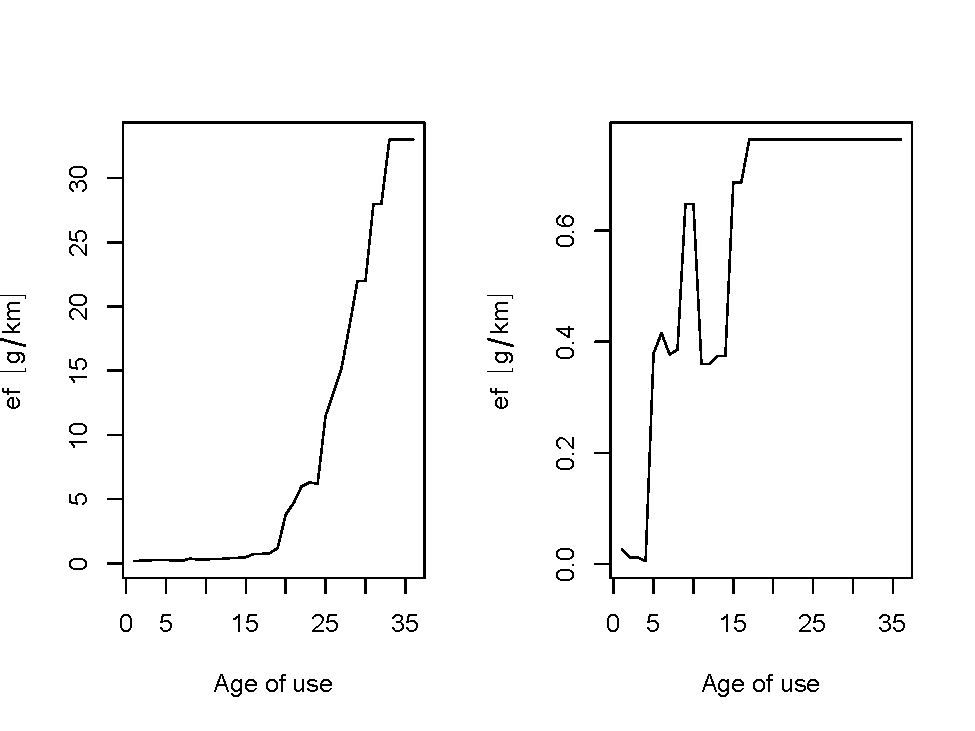
\includegraphics[width=0.8\linewidth]{veinbook_files/figure-latex/efco-1} 

}

\caption{Emission factor of PC and LT by age of use}\label{fig:efco}
\end{figure}

Regarding the class \texttt{EmissionFactorsList}, the \texttt{print} and
\texttt{summary} methods are straightforward, only showing a description
of the object. The example of the following lines of code also uses the
same set of Emission Factors from \citet{CETESB2015}. The resulting
object, EF\_COL, is of class \texttt{EmissionFactorsList} and
\texttt{list}. The print of the object shows only a description of the
first and last member of the list object.

\begin{Shaded}
\begin{Highlighting}[]
\NormalTok{EFL_CO <-}\StringTok{ }\KeywordTok{EmissionFactorsList}\NormalTok{(DF_CO)}
\KeywordTok{class}\NormalTok{(EFL_CO)}
\end{Highlighting}
\end{Shaded}

\begin{verbatim}
## [1] "EmissionFactorsList" "data.frame"
\end{verbatim}

\begin{Shaded}
\begin{Highlighting}[]
\NormalTok{EFL_CO}
\end{Highlighting}
\end{Shaded}

\begin{verbatim}
## This EmissionFactorsList has  2  lists
## First has  36  functions
## Last has  36  functions
\end{verbatim}

Indeed, if we want to see the content of the
\texttt{EmissionFactorsList} we have to extract the elements of the
list. EFL\_CO has two lists; one for PC and one for LT. Then, each list
has 36 functions, the command
\texttt{class(EFL\_CO{[}{[}1{]}{]}{[}{[}1{]}{]})} shows the object is a
function \(f(V)\).

\begin{Shaded}
\begin{Highlighting}[]
\NormalTok{EFL_CO[[}\DecValTok{1}\NormalTok{]][[}\DecValTok{1}\NormalTok{]]}
\end{Highlighting}
\end{Shaded}

\begin{verbatim}
## function(V) x[j,i]
## <bytecode: 0x5630d2848200>
## <environment: 0x5630e3d33ce8>
\end{verbatim}

Also, as the speed functions are constant, there is no need to add
values of V.

\begin{Shaded}
\begin{Highlighting}[]
\NormalTok{EFL_CO[[}\DecValTok{1}\NormalTok{]][[}\DecValTok{1}\NormalTok{]](}\DecValTok{100}\NormalTok{) }\CommentTok{# constant speed function}
\end{Highlighting}
\end{Shaded}

\begin{verbatim}
## [1] 0.171
\end{verbatim}

\begin{Shaded}
\begin{Highlighting}[]
\NormalTok{EFL_CO[[}\DecValTok{1}\NormalTok{]][[}\DecValTok{1}\NormalTok{]](}\DecValTok{0}\NormalTok{)   }\CommentTok{# constant speed function}
\end{Highlighting}
\end{Shaded}

\begin{verbatim}
## [1] 0.171
\end{verbatim}

Finally, after extracting the value, Fig. (\ref{fig:efco2}) shows the
same figure as Fig. (\ref{fig:efco})

\begin{Shaded}
\begin{Highlighting}[]
\NormalTok{efco1 <-}\StringTok{ }\KeywordTok{sapply}\NormalTok{(}\DecValTok{1}\OperatorTok{:}\DecValTok{36}\NormalTok{, }\ControlFlowTok{function}\NormalTok{(i) EFL_CO[[}\DecValTok{1}\NormalTok{]][[i]]())}
\NormalTok{efco2 <-}\StringTok{ }\KeywordTok{sapply}\NormalTok{(}\DecValTok{1}\OperatorTok{:}\DecValTok{36}\NormalTok{, }\ControlFlowTok{function}\NormalTok{(i) EFL_CO[[}\DecValTok{2}\NormalTok{]][[i]]())}
\NormalTok{df <-}\StringTok{ }\KeywordTok{EmissionFactors}\NormalTok{(}\KeywordTok{cbind}\NormalTok{(efco1, efco2))}
\KeywordTok{plot}\NormalTok{(df, }\DataTypeTok{xlab =} \StringTok{"Age of use"}\NormalTok{)}
\end{Highlighting}
\end{Shaded}

\begin{figure}

{\centering 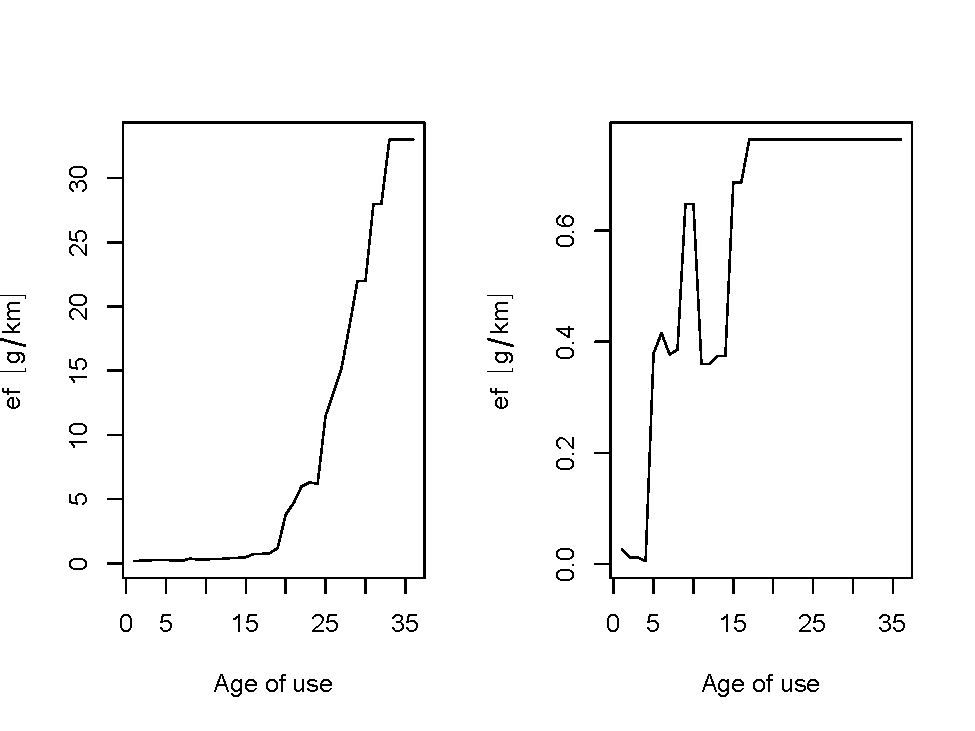
\includegraphics[width=0.8\linewidth]{veinbook_files/figure-latex/efco2-1} 

}

\caption{Emission factor of PC and LT}\label{fig:efco2}
\end{figure}

\section{\texorpdfstring{Incorporating speed variation with the
functions \texttt{ef\_ldv\_scaled} and
\texttt{ef\_hdv\_scaled}}{Incorporating speed variation with the functions ef\_ldv\_scaled and ef\_hdv\_scaled}}\label{scale}

The functions in section \ref{speedef} and \ref{localef} showed the
speed and local emission factors respectively. However, the user might
have local and constant emission factors depending only on the age of
use, but also, outputs from a traffic demand model which includes speed.
Under those circumstances, it would be interesting to investigate the
effects of the average rate of traffic flow. VEIN provides for functions
to transform a constant emission factor by the age of use into a speed
dependent function.

These functions are called \texttt{ef\_ldv\_scaled} and
\texttt{ef\_hdv\_scaled}. The concept is explained in detail in my
Ph.D.~thesis \citep{ibarrathesis}. The idea comes from revisiting the
nature of the local emission factors. The Brazilian emission factors
consist of average measurements for emissions certification tests which
use the driving cycles Federal Test Procedure FTP-75 for LDV, World
Motorcycle Test Cycle (WMTC) for motorcycles, and also the European
Stationary Cycle (ESC) for HDV \citep{CETESB2015}. The average speed of
FTP-75 and WMTC are known, being 34.2 \(km \cdot h^{-1}\) and 54.7
\(km \cdot h^{-1}\) based on the reference report on driving cycles from
the Transport and Research Laboratory (TRL) \citep{tim}. In the case of
ESC, the user might search on literature a way to relate this cycle with
an average speed.

Coming back to the \citet{CETESB2015} emission factors, these are annual
average values of emissions for the different technologies to accomplish
Brazilian emission standards, which are valid only for a specific
average speed. If two vehicles have similar technology but different
emission factors, one constant and other speed function, it would be
possible to relate them. These functions use the speed to relate both
emission factors. The condition to transform a constant emission factor
into a speed dependent function is that the new speed-dependent function
must be of the same value at the speed which is representative for the
local factor, And the values at other speeds are the incorporation of
the speed variation. The equation \eqref{eq:efscaled} shows the procedure:

\begin{equation}
EF_{scaled}(V_{i,l})_{j,k,m}=EF(V_{i,l})_{j,k,m} \cdot \frac{EFlocal_{j,k,m}}{{EF(Vdc_{i,l})_{j,k,m}}}
\label{eq:efscaled}
\end{equation}

Where \(EF_{scaled}(V_{i,l})_{j,k,m}\) is the scaled emission factor and
\(EF(V_{i,l})_{j,k,m}\) is the Copert emission factor for each street
link \(i\), vehicle from composition \(k\), hour \(l\) and pollutant
\(m\). \(EFlocal_{j,k,m}\) represents the constant emission factor (not
as speed functions). \(EF(Vdc_{i,l})_{j,k,m}\) are Copert emission
factors with average speed value of the respective driving cycle for the
vehicular category \(j\).

The functions \texttt{ef\_ldv\_scaled} and \texttt{ef\_hdv\_scaled}
return scaled emissions factors automatically. The arguments are:

\begin{Shaded}
\begin{Highlighting}[]
\KeywordTok{args}\NormalTok{(ef_ldv_scaled)}
\end{Highlighting}
\end{Shaded}

\begin{verbatim}
## function (df, dfcol, SDC = 34.12, v, t = "4S", cc, f, eu, p) 
## NULL
\end{verbatim}

\begin{itemize}
\tightlist
\item
  \texttt{df}: Data-frame with emission factors (Deprecated in 0.3.10).
\item
  \texttt{dfcol}: Numeric vector with the emission factors constant by
  age of use. These emission factors are the target to incorporate speed
  variation.
\item
  \texttt{SDC}: A number with the speed of the driving cycle of the
  emission factors from the argument \texttt{dfcol}. The resulting speed
  functions will return the same values of dfcol at the speed
  \texttt{SDC}. The default is 34.12 ``km/h''.
\item
  \texttt{v}. Category of vehicle: ``PC'', ``LCV'', ``Motorcycle'' or
  ``Moped''.
\item
  \texttt{t}. Character; sub-category of vehicle: PC: ``ECE\_1501'',
  ``ECE\_1502'', ``ECE\_1503'', ``ECE\_1504'' ,
  ``IMPROVED\_CONVENTIONAL'', ``OPEN\_LOOP'', ``ALL'', ``2S'' or ``4S''.
  LCV: ``4S'', Motorcycle: ``2S'' or ``4S''. Moped: ``2S'' or ``4S''.
  The default is \texttt{4S}.
\item
  \texttt{cc}. Character; size of engine in cc: PC:
  ``\textless{}=1400'', ``\textgreater{}1400'', ``1400\_2000'',
  ``\textgreater{}2000'', ``\textless{}=800'', ``\textless{}=2000''.
  Motorcycle: ``\textgreater{}=50'' (for ``2S''), ``\textless{}=250'',
  ``250\_750'', ``\textgreater{}=750''. Moped: ``\textless{}=50''. LCV :
  ``\textless{}3.5'' for gross weight.
\item
  \texttt{f}: Character; type of fuel: ``G'', ``D'', ``LPG'' or ``FH''
  (Full Hybrid: starts by electric motor).
\item
  \texttt{eu}: Character; euro standard: ``PRE'', ``I'', ``II'',
  ``III'', ``III+DPF'', ``IV'', ``V'', ``VI'' or ``VIc''.
\item
  \texttt{p}: Character; pollutant: ``CO'', ``FC'', ``NOx'', ``HC'' or
  ``PM''.
\end{itemize}

And the argument of \texttt{ef\_hdv\_scaled} are:

\begin{Shaded}
\begin{Highlighting}[]
\KeywordTok{args}\NormalTok{(ef_hdv_scaled)}
\end{Highlighting}
\end{Shaded}

\begin{verbatim}
## function (df, dfcol, SDC = 34.12, v, t, g, eu, gr = 0, l = 0.5, 
##     p) 
## NULL
\end{verbatim}

\begin{itemize}
\tightlist
\item
  \texttt{df}: Data-frame with emission factors (Deprecated in 0.3.10).
\item
  \texttt{dfcol}: Numeric vector with the emission factors constant by
  age of use. - \texttt{SDC} Speed of the driving cycle.
\item
  \texttt{v}: Category vehicle: ``Coach'', ``Trucks'' or ``Ubus''
\item
  \texttt{t}: Sub-category of of vehicle: ``3Axes'', ``Artic'',
  ``Midi'', ``RT,''Std" and ``TT''
\item
  \texttt{g}: Gross weight of each category: ``\textless{}=18'',
  ``\textgreater{}18'', ``\textless{}=15'', ``\textgreater{}15 \&
  \textless{}=18'', ``\textless{}=7.5'', ``\textgreater{}7.5 \&
  \textless{}=12'', ``\textgreater{}12 \& \textless{}=14'',
  ``\textgreater{}14 \& \textless{}=20'', ``\textgreater{}20 \&
  \textless{}=26'', ``\textgreater{}26 \& \textless{}=28'',
  ``\textgreater{}28 \& \textless{}=32'', ``\textgreater{}32'',
  ``\textgreater{}20 \& \textless{}=28'', ``\textgreater{}28 \&
  \textless{}=34'', ``\textgreater{}34 \& \textless{}=40'',
  ``\textgreater{}40 \& \textless{}=50'' or ``\textgreater{}50 \&
  \textless{}=60''
\item
  \texttt{eu}: Euro emission standard: ``PRE'', ``I'', ``II'', ``III'',
  ``IV'' and ``V''
\item
  \texttt{gr}: Gradient or slope of road: -0.06, -0.04, -0.02, 0.00,
  0.02. 0.04 or 0.06
\item
  \texttt{l}: Load of the vehicle: 0.0, 0.5 or 1.0
\item
  \texttt{p}: Pollutant: ``CO'', ``FC'', ``NOx'' or ``HC''
\end{itemize}

\section{Cold Starts}\label{cold-starts}

Cold start emissions are produced during engine startup when the engine
and catalytic converter system has not reached its normal operating
temperature. Several studies have shown a significant impact on these
types of emissions \citep[\citet{Weilenmannetal2009}]{chenetal2011}.
Under this condition emissions will be higher, and if the atmospheric
temperature decreases, cold start emissions will increase regardless of
whether the catalyst has reached its optimum temperature for functioning
\citep{artemis}. VEIN also considers cold start emissions using the
approach outlined in Copert \citep{NtziachristosSamaras2016}, as shown
in equation \eqref{eq:cold}.

\begin{equation}
EC_{i,j,k,l,m} =\beta_{j} \cdot F_{i,j,k,l} \cdot L_i \cdot EF(V_{i,l})_{j,k,m} \cdot DF_{j.k} \cdot \left(EF_{\mbox{cold}}(ta_n,V_{i,l})_{j,k,m}-1\right)
\label{eq:cold}
\end{equation}

This approach adds two terms to Eq. \ref{eq:emi}. The first term
\(EF_{cold}(ta_n,V_{i,l})_{j,k,m}-1\) is the emission factors for cold
start conditions at each street link \(i\), vehicle category from
composition \(k\), hour \(l\) and pollutant \(m\) and monthly average
temperature \(n\). \citep{NtziachristosSamaras2016} suggest using
monthly average temperature.

The second term \(\beta_j\) is defined as the fraction of mileage driven
with a cold engine/catalyst \citep{NtziachristosSamaras2016}. The VEIN
model incorporates a dataset of cold starts recorded during the
implementation of the International Vehicle Emissions (IVE) model
\citep{Davisetal2005} in São Paulo \citep{ivesp}, which provides the
hourly mileage driven with cold start conditions.

The function for cold start emission factors is \texttt{ef\_ldv\_cold}
and its arguments are:

\begin{Shaded}
\begin{Highlighting}[]
\KeywordTok{args}\NormalTok{(ef_ldv_cold)}
\end{Highlighting}
\end{Shaded}

\begin{verbatim}
## function (v = "LDV", ta, cc, f, eu, p, k = 1, show.equation = FALSE) 
## NULL
\end{verbatim}

where:

\begin{itemize}
\tightlist
\item
  \texttt{v}: Category of vehicle: ``LDV''.
\item
  \texttt{ta}: Ambient temperature. Monthly mean can be used.
\item
  \texttt{cc}: Size of engine in cc: ``\textless{}=1400'',
  ``1400\_2000'' or ``\textgreater{}2000''.
\item
  \texttt{f}: Type of fuel: ``G'', ``D'' or ``LPG''.
\item
  \texttt{eu}: Euro standard: ``PRE'', ``I'', ``II'', ``III'', ``IV'',
  ``V'', ``VI'' or ``VIc''.
\item
  \texttt{p}: Pollutant: ``CO'', ``FC'', ``NOx'', ``HC'' or ``PM''.
\item
  \texttt{k}: Multiplication factor.
\item
  \texttt{show.equation}: Option to see or not the equation parameters.
\end{itemize}

\begin{Shaded}
\begin{Highlighting}[]
\NormalTok{ef1 <-}\StringTok{ }\KeywordTok{ef_ldv_cold}\NormalTok{(}\DataTypeTok{ta =} \DecValTok{-5}\NormalTok{, }\DataTypeTok{cc =} \StringTok{"<=1400"}\NormalTok{, }\DataTypeTok{f =}\StringTok{"G"}\NormalTok{, }\DataTypeTok{eu =} \StringTok{"I"}\NormalTok{, }\DataTypeTok{p =} \StringTok{"CO"}\NormalTok{)}
\NormalTok{ef2 <-}\StringTok{ }\KeywordTok{ef_ldv_cold}\NormalTok{(}\DataTypeTok{ta =} \DecValTok{0}\NormalTok{, }\DataTypeTok{cc =} \StringTok{"<=1400"}\NormalTok{, }\DataTypeTok{f =}\StringTok{"G"}\NormalTok{, }\DataTypeTok{eu =} \StringTok{"I"}\NormalTok{, }\DataTypeTok{p =} \StringTok{"CO"}\NormalTok{)}
\NormalTok{ef3 <-}\StringTok{ }\KeywordTok{ef_ldv_cold}\NormalTok{(}\DataTypeTok{ta =} \DecValTok{5}\NormalTok{, }\DataTypeTok{cc =} \StringTok{"<=1400"}\NormalTok{, }\DataTypeTok{f =}\StringTok{"G"}\NormalTok{, }\DataTypeTok{eu =} \StringTok{"I"}\NormalTok{, }\DataTypeTok{p =} \StringTok{"CO"}\NormalTok{)}
\NormalTok{ef4 <-}\StringTok{ }\KeywordTok{ef_ldv_cold}\NormalTok{(}\DataTypeTok{ta =} \DecValTok{10}\NormalTok{, }\DataTypeTok{cc =} \StringTok{"<=1400"}\NormalTok{, }\DataTypeTok{f =}\StringTok{"G"}\NormalTok{, }\DataTypeTok{eu =} \StringTok{"I"}\NormalTok{, }\DataTypeTok{p =} \StringTok{"CO"}\NormalTok{)}
\end{Highlighting}
\end{Shaded}

\begin{figure}

{\centering 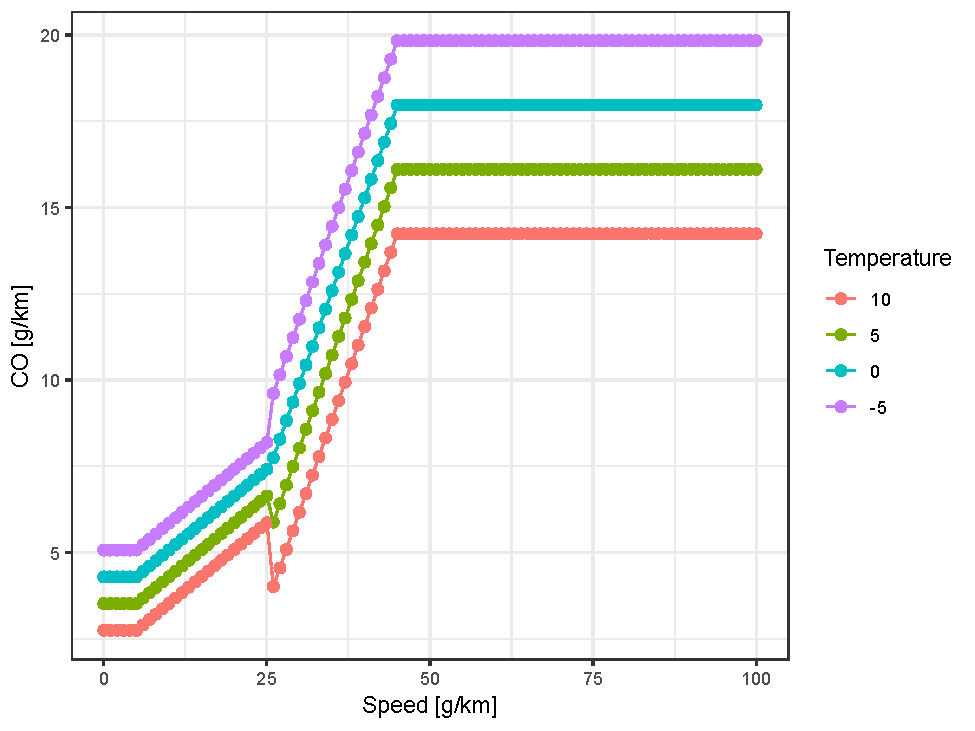
\includegraphics[width=0.8\linewidth]{veinbook_files/figure-latex/efcold-1} 

}

\caption{Cold Emission factor of PC CO (g/km)}\label{fig:efcold}
\end{figure}

There is another function called \texttt{ef\_ldv\_cold\_list} which will
be deprecated soon.

\section{Deterioration}\label{det}

By default, VEIN includes deterioration factors from Copert
\citep{NtziachristosSamaras2016}. However, it is possible to include
other sources, such as from \citep{CorvalanVargas2003} or includes
deteriorated local emission factors. This aspect is faced in VEIN with
the function \texttt{emis\_det}. This function returns deteriorated
factors, as numeric vectors, which must be multiplied with the emission
factors of vehicles with 0 mileage.

The arguments of this functions are:

\begin{Shaded}
\begin{Highlighting}[]
\KeywordTok{args}\NormalTok{(emis_det)}
\end{Highlighting}
\end{Shaded}

\begin{verbatim}
## function (po, cc, eu, km) 
## NULL
\end{verbatim}

where:

\begin{itemize}
\tightlist
\item
  \texttt{p}: Pollutant.
\item
  \texttt{cc}: Size of an engine in cc.
\item
  \texttt{eu}: Euro standard: ``PRE'', ``I'', ``II'', ``III'', ``III'',
  ``IV'', ``V'', ``VI''.
\item
  \texttt{km}: mileage in km. VEIN includes a dataset of mileage
  function named ``fkm''.
\end{itemize}

\begin{Shaded}
\begin{Highlighting}[]
\KeywordTok{data}\NormalTok{(fe2015)}
\KeywordTok{data}\NormalTok{(fkm)}
\NormalTok{pckma <-}\StringTok{ }\KeywordTok{cumsum}\NormalTok{(fkm}\OperatorTok{$}\KeywordTok{KM_PC_E25}\NormalTok{(}\DecValTok{1}\OperatorTok{:}\DecValTok{24}\NormalTok{)) }\CommentTok{#only vehicles with catalizer}
\NormalTok{x1 <-}\StringTok{ }\NormalTok{fe2015[fe2015}\OperatorTok{$}\NormalTok{Pollutant }\OperatorTok{==}\StringTok{ "CO"}\NormalTok{, ]}
\NormalTok{x1E3 <-}\StringTok{ }\KeywordTok{subset}\NormalTok{(x1, x1}\OperatorTok{$}\NormalTok{Euro_LDV }\OperatorTok\StringTok{ }\KeywordTok{c}\NormalTok{(}\StringTok{"III"}\NormalTok{, }\StringTok{"IV"}\NormalTok{, }\StringTok{"V"}\NormalTok{))}\OperatorTok{$}\NormalTok{PC_G}
\NormalTok{x1E1 <-}\StringTok{ }\KeywordTok{subset}\NormalTok{(x1, x1}\OperatorTok{$}\NormalTok{Euro_LDV }\OperatorTok\StringTok{ }\KeywordTok{c}\NormalTok{(}\StringTok{"I"}\NormalTok{, }\StringTok{"II"}\NormalTok{))}\OperatorTok{$}\NormalTok{PC_G}
\NormalTok{det_E3 <-}\StringTok{ }\KeywordTok{emis_det}\NormalTok{(}\DataTypeTok{po =} \StringTok{"CO"}\NormalTok{, }\DataTypeTok{cc =} \DecValTok{1000}\NormalTok{, }\DataTypeTok{eu =} \StringTok{"III"}\NormalTok{,}
                   \DataTypeTok{km =}\NormalTok{ pckma[}\DecValTok{1}\OperatorTok{:}\KeywordTok{length}\NormalTok{(x1E3)])}
\NormalTok{det_E1 <-}\StringTok{ }\KeywordTok{emis_det}\NormalTok{(}\DataTypeTok{po =} \StringTok{"CO"}\NormalTok{, }\DataTypeTok{cc =} \DecValTok{1000}\NormalTok{, }\DataTypeTok{eu =} \StringTok{"III"}\NormalTok{,}
                   \DataTypeTok{km =}\NormalTok{ pckma[(}\KeywordTok{length}\NormalTok{(x1E3) }\OperatorTok{+}\StringTok{ }\DecValTok{1}\NormalTok{)}\OperatorTok{:}\DecValTok{23}\NormalTok{ ])}
\NormalTok{original_EF <-}\StringTok{ }\NormalTok{x1}\OperatorTok{$}\NormalTok{PC}
\NormalTok{deteriorated_EF <-}\StringTok{ }\NormalTok{x1}\OperatorTok{$}\NormalTok{PC }\OperatorTok{*}\StringTok{ }\KeywordTok{c}\NormalTok{(det_E3, det_E1, }\KeywordTok{rep}\NormalTok{(}\DecValTok{1}\NormalTok{, }\DecValTok{13}\NormalTok{))}
\KeywordTok{plot}\NormalTok{(}\DataTypeTok{x =} \DecValTok{1}\OperatorTok{:}\DecValTok{36}\NormalTok{, }\DataTypeTok{y =}\NormalTok{ original_EF, }\DataTypeTok{type =} \StringTok{"b"}\NormalTok{, }\DataTypeTok{pch =} \DecValTok{15}\NormalTok{, }\DataTypeTok{col =} \StringTok{"blue"}\NormalTok{,}
     \DataTypeTok{ylab =} \StringTok{"CO[g/km]"}\NormalTok{, }\DataTypeTok{xlab =} \StringTok{"Age of use"}\NormalTok{)}
\CommentTok{#     main = "Deteriorated (red) and not-deteriorated (blue) EF CO")}
\KeywordTok{lines}\NormalTok{(}\DataTypeTok{x =} \DecValTok{1}\OperatorTok{:}\DecValTok{36}\NormalTok{, }\DataTypeTok{y =}\NormalTok{ deteriorated_EF,  }\DataTypeTok{type =} \StringTok{"b"}\NormalTok{, }\DataTypeTok{pch =} \DecValTok{16}\NormalTok{, }\DataTypeTok{col =} \StringTok{"red"}\NormalTok{)}
\end{Highlighting}
\end{Shaded}

\begin{figure}

{\centering 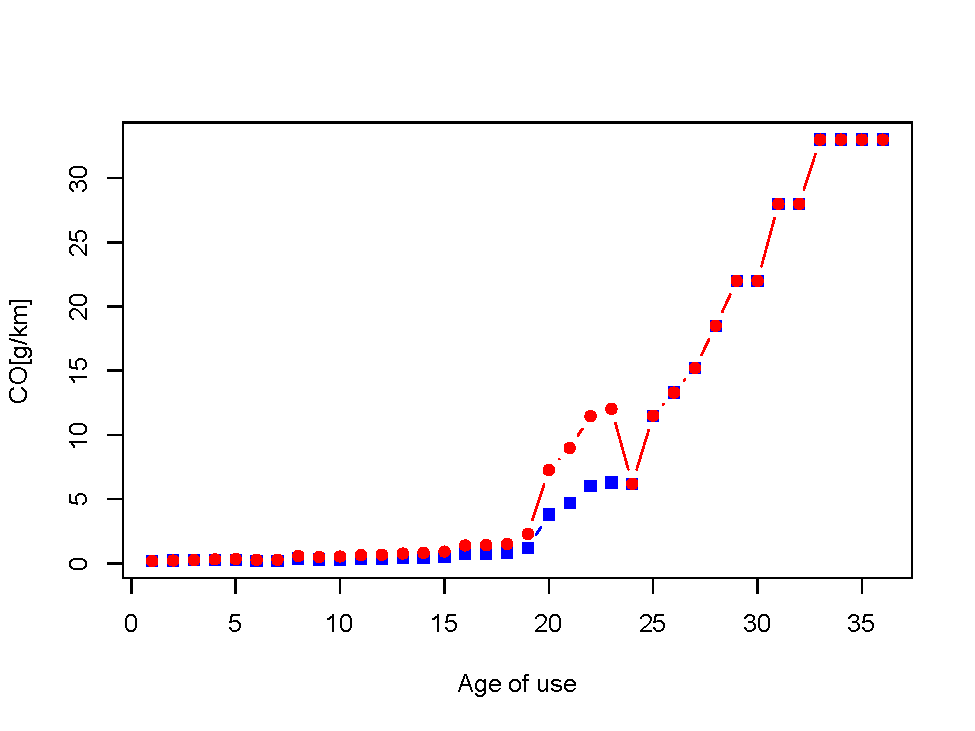
\includegraphics[width=0.8\linewidth]{veinbook_files/figure-latex/efDET-1} 

}

\caption{Deteriorated (red) and not-deteriorated (blue) EF CO}\label{fig:efDET}
\end{figure}

\section{\texorpdfstring{Evaporative emissions
\texttt{ef\_evap}}{Evaporative emissions ef\_evap}}\label{evaporative-emissions-ef_evap}

Evaporative emissions are essential sources of hydrocarbons, and these
emissions are produced by vaporization of fuel due to variations in
ambient temperatures
\citep[\citet{Andradeetal2017}]{MelliosNtziachristos2016}. There are
three types of emissions: \textbf{diurnal emissions}, due to increases
in atmospheric temperature, which lead to the thermal expansion of vapor
fuel inside the tank; \textbf{running losses}, when the fuel evaporates
inside the tank due to the normal operation of the vehicle; and
\textbf{hot soak} emissions, which occur when the hot engine is turned
off. These methods implemented in VEIN were sourced from the evaporative
emissions methods of Copert Tier 2 \citep{MelliosNtziachristos2016}. In
VEIN it is also possible to use local emission factors. Here I'm showing
both approaches:

\begin{enumerate}
\def\labelenumi{\alph{enumi})}
\tightlist
\item
  Tier 2 copert approach
\end{enumerate}

\begin{equation}
EV_{j,k} =\sum_{s}D_{s} \cdot \sum_{j}F_{j} \cdot (HS_{j,k}+de_{j,k}+RL_{j,k}) 
\label{eq:ev1}
\end{equation}

where \(EV_{j}\) are the volatile organic compounds (VOC) evaporative
emissions due to each type of vehicle \(j\). \(D_s\) is the ``seasonal
days'' or number of days when the mean monthly temperature is within a
determined range: {[}-5\(^{\circ}\),10\(^{\circ}\)C{]},
{[}0\(^{\circ}\), 15\(^{\circ}\)C{]}, {[}10\(^{\circ}\),
25\(^{\circ}\)C{]} and {[}20\(^{\circ}\), 35\(^{\circ}\)C{]}.
\(F_{j,k}\) is the number of vehicles according to the same type \(j\)
and age of use \(k\). \(HS_{j,k}\), \(de_{j,k}\) and \(RL_{j,k}\) are
average hot/warm soak, diurnal and running losses evaporative emissions
(\(\mathrm{g \cdot day^{-1}}\)), respectively, according to the vehicle
type \(j\) and age of use \(k\). \(HS_{j,k}\) and \(RL_{j,k}\) are
obtained using equations also sourced from
\citep{MelliosNtziachristos2016}:

\begin{equation}
HS_{j,k} = x_{j,k} \cdot (c \cdot (p \cdot e_{shc}+(1-p) \cdot e_{swc})+(1-c) \cdot e_{shfi} )
\label{eq:ev2}
\end{equation}

where: \(x\) is the number of trips per day for the vehicular type \(j\)
and age of use \(k\). \(c\) is the fraction of vehicles with fuel return
systems. \(p\) is the fraction of trips finished with a hot engine, for
example, an engine that has reached its normal operating temperature and
the catalyst has reached its light-off temperature
\citep{NtziachristosSamaras2016}. The light-off temperature is the
temperature at the point when catalytic reactions occur inside a
catalytic converter. \(e_{shc}\) and \(e_{swc}\) are average hot-soak
and warm-soak emission factors for gasoline vehicles with carburettor or
fuel return systems (\(\mathrm{g \cdot parking^{-1}}\)). \(e_{shfi}\) is
the average hot-soak emission factors for gasoline vehicles equipped
with fuel injection and non-return fuel systems
(\(\mathrm{g \cdot parking^{-1}}\)).

The Eq. \eqref{eq:ev3} shows the procedure.

\begin{equation}
RL_{j,k} = x_{j,k} \cdot (c \cdot (p \cdot e_{rhc}+(1-p) \cdot e_{rwc})+(1-c) \cdot e_{rhfi} )
\label{eq:ev3}
\end{equation}

where: \(x\) and \(p\) have the same meanings of Eq. \eqref{eq:ev2}.
\(e_{rhc}\) and \(e_{rwc}\) are average hot and warm running losses
emission factors for gasoline vehicles with carburettor or fuel return
systems (\(\mathrm{g \cdot trip^{-1}}\)) \(e_{rhfi}\) are average hot
running losses emission factors for gasoline vehicles equipped withfuel
injection and non-return fuel systems (\(\mathrm{g \cdot trip^{-1}}\)).

It is recommended to estimate the number of trips per day
\citep{MelliosNtziachristos2016}, \(x\), as the division between the
mileage and 365 times the length of trip:
\(x = \frac{mileage_j}{(365 \cdot ltrip)}\).

However, the mileage of a vehicle is not constant throughout the years.
Therefore, VEIN incorporates a dataset of equations to estimate mileage
of different types of cars by the age of use \citep{BruniBales2013}.

The function for evaporative emission factors is \texttt{ef\_evap} and
it arguments are :

\begin{Shaded}
\begin{Highlighting}[]
\KeywordTok{args}\NormalTok{(ef_evap)}
\end{Highlighting}
\end{Shaded}

\begin{verbatim}
## function (ef, v, cc, dt, ca, k = 1, show = FALSE) 
## NULL
\end{verbatim}

where: - \texttt{ef}: Name of evaporative emission factor as
\emph{eshotc} (\(g \cdot proced^-1\)): mean hot-soak with carburator,
\emph{eswarmc} (\(g \cdot proced^-1\)): mean cold and warm-soak with
carburator, \emph{eshotfi}: mean hot-soak with fuel injection,
\emph{erhotc} (\(g \cdot trip^-1\)): mean hot running losses with
carburator, \emph{erwarmc} (\(g \cdot trip^-1\)) mean cold and warm
running losses, \emph{erhotfi} (\(g \cdot trip^-1\)) mean hot running
losses with fuel injection. - \texttt{v}: Type of vehicles, ``PC'',
``Motorcycles'', ``Motorcycles\_2S'' and ``Moped'' - \texttt{cc}: Size
of engine in cc. PC ``\textless{}=1400'', ``1400\_2000'' and ``2000''
Motorcycles\_2S: ``\textless{}=50''. Motorcyces: ``\textgreater{}50'',
``\textless{}250'', ``250\_750'' and ``\textgreater{}750'' -
\texttt{dt}: Average daily temperature variation: ``-5\_10'', ``0\_15'',
``10\_25'' and ``20\_35'' - \texttt{ca}: Size of canister: ``no''
meaning no canister, ``small'', ``medium'' and ``large'' - \texttt{k}:
multiplication factor - \texttt{show}: when TRUE shows row of table with
respective emission factor.

Example:

\begin{Shaded}
\begin{Highlighting}[]
\KeywordTok{library}\NormalTok{(vein)}
\KeywordTok{library}\NormalTok{(ggplot2)}
\KeywordTok{library}\NormalTok{(cptcity)}
\NormalTok{dt <-}\StringTok{ }\KeywordTok{c}\NormalTok{(}\StringTok{"-5_10"}\NormalTok{, }\StringTok{"0_15"}\NormalTok{, }\StringTok{"10_25"}\NormalTok{, }\StringTok{"20_35"}\NormalTok{)}
\NormalTok{ef <-}\StringTok{ }\KeywordTok{sapply}\NormalTok{(}\DecValTok{1}\OperatorTok{:}\DecValTok{4}\NormalTok{, }\ControlFlowTok{function}\NormalTok{(i)\{}
  \KeywordTok{ef_evap}\NormalTok{(}\DataTypeTok{ef =} \StringTok{"erhotc"}\NormalTok{,}\DataTypeTok{v =} \StringTok{"PC"}\NormalTok{, }\DataTypeTok{cc =} \StringTok{"<=1400"}\NormalTok{,}
                \DataTypeTok{dt =}\NormalTok{ dt[i], }\DataTypeTok{ca =} \StringTok{"no"}\NormalTok{,}
                \DataTypeTok{show =} \OtherTok{TRUE}\NormalTok{)}
\NormalTok{\})}
\end{Highlighting}
\end{Shaded}

\begin{verbatim}
##        ef  units veh     cc    dt canister    g
## 28 erhotc g/trip  PC <=1400 -5_10       no 1.67
##        ef  units veh     cc   dt canister    g
## 21 erhotc g/trip  PC <=1400 0_15       no 2.39
##        ef  units veh     cc    dt canister    g
## 14 erhotc g/trip  PC <=1400 10_25       no 3.25
##       ef  units veh     cc    dt canister    g
## 7 erhotc g/trip  PC <=1400 20_35       no 5.42
\end{verbatim}

\begin{Shaded}
\begin{Highlighting}[]
\NormalTok{df <-}\StringTok{ }\KeywordTok{data.frame}\NormalTok{(}\DataTypeTok{ef =}\NormalTok{ ef, }\DataTypeTok{temp =} \KeywordTok{c}\NormalTok{(}\DecValTok{0}\NormalTok{, }\DecValTok{10}\NormalTok{, }\DecValTok{20}\NormalTok{, }\DecValTok{30}\NormalTok{))}
\KeywordTok{source}\NormalTok{(}\StringTok{"theme_black.R"}\NormalTok{)}
\KeywordTok{ggplot}\NormalTok{(df, }\KeywordTok{aes}\NormalTok{(}\DataTypeTok{x =}\NormalTok{ temp, }\DataTypeTok{y =}\NormalTok{ ef)) }\OperatorTok{+}
\StringTok{  }\KeywordTok{geom_bar}\NormalTok{(}\DataTypeTok{stat =} \StringTok{"identity"}\NormalTok{, }\DataTypeTok{fill =} \KeywordTok{cpt}\NormalTok{(}\DataTypeTok{n =} \DecValTok{4}\NormalTok{), }\DataTypeTok{col =} \StringTok{"white"}\NormalTok{) }\OperatorTok{+}\StringTok{ }
\StringTok{  }\KeywordTok{labs}\NormalTok{(}\DataTypeTok{x =} \StringTok{"Temperature[C]"}\NormalTok{, }\DataTypeTok{y =} \StringTok{"RL Evaporative NMHC [g/trip]"}\NormalTok{) }\OperatorTok{+}\StringTok{ }
\StringTok{  }\KeywordTok{theme_black}\NormalTok{()}
\end{Highlighting}
\end{Shaded}

\begin{figure}

{\centering 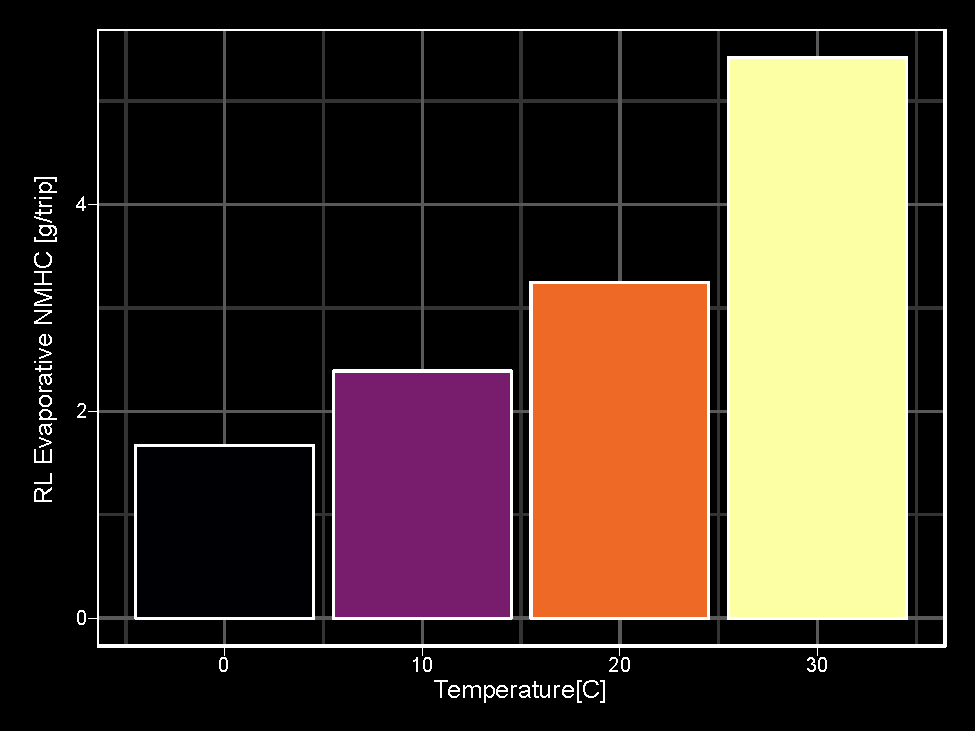
\includegraphics[width=1\linewidth]{veinbook_files/figure-latex/rlevap-1} 

}

\caption{Running losses evaporative emission actors (g/trip)}\label{fig:rlevap}
\end{figure}

\begin{enumerate}
\def\labelenumi{\alph{enumi})}
\setcounter{enumi}{1}
\tightlist
\item
  Alternative approach
\end{enumerate}

The evaporative emission factors mentioned before are suitable for
top-down estimations. That approach also requires knowledge of the
`procedure' and `trips'. In this section it is introduced an alternative
which consists in transform the emission factors into \(g \cdot km^-1\)
and then do a bottom-up estimation.

To do that, we need to follow some assumptions. First, we consider that
the number of procedures is equal to trips. Then I estimated how many
trips per day each day, and then we estimate how many kilometers are
driven each day and convert these to emission factors as shown on Eq.
\eqref{eq:efev2}.

\begin{equation}
EF_{ev}(\frac{g}{km})=EF(_{ev})(\frac{g}{trip}) \cdot A(\frac{trips}{day}) \cdot B(\frac{km}{day})^{-1}
\label{eq:efev2}
\end{equation}

Clearly, we need to know A \((\frac{trips}{day})\) and
B\((\frac{km}{day})^{-1}\). Diurnal evaporative emissions factors are
expressed as \((\frac{g}{day})\). To convert to \((\frac{g}{km})\) we
only need the kilometers driven each day \(\frac{km}{day}^{-1}\).

Now, it will be shown an example of the evaporative emission factors
from \citet{CETESB2015}. These emission factors are based on the
methodology Tier 2 from -@\citet{MelliosNtziachristos2016}. If we
consider evaporative emission factors of Passenger Cars using Gasoline
(blended with 25\% of Ethanol) \citep{CETESB2015} and4.6
\((\frac{trips}{day})\) \citep{ibarrathesis}.

\begin{verbatim}
##   year ed_20_35 eshot_20_35 erhot_20_35
## 1 2015     0.06        0.09        0.03
## 2 2014     0.10        0.10        0.04
## 3 2013     0.12        0.13        0.05
## 4 2012     0.19        0.16        0.06
## 5 2011     0.19        0.17        0.14
## 6 2010     0.08        0.08        0.06
\end{verbatim}

The variable ed\_20\_35 are diurnal evaporative emission factors in
\(g \cdot day^{-1}\) and eshot\_20\_35 and erhot\_20\_35
\(g \cdot trip^{-1}\).

\begin{Shaded}
\begin{Highlighting}[]
\KeywordTok{library}\NormalTok{(vein)}
\KeywordTok{data}\NormalTok{(fkm)}
\NormalTok{evap}\OperatorTok{$}\NormalTok{ed_}\DecValTok{20}\NormalTok{_}\DecValTok{35}\NormalTok{_gkm <-}\StringTok{ }\NormalTok{evap}\OperatorTok{$}\NormalTok{ed_}\DecValTok{20}\NormalTok{_}\DecValTok{35} \OperatorTok{/}\StringTok{ }\NormalTok{fkm}\OperatorTok{$}\KeywordTok{KM_PC_E25}\NormalTok{(}\DecValTok{1}\OperatorTok{:}\DecValTok{41}\NormalTok{)}\OperatorTok{/}\DecValTok{365}
\NormalTok{evap}\OperatorTok{$}\NormalTok{eshot_}\DecValTok{20}\NormalTok{_}\DecValTok{35}\NormalTok{_gkm <-}\StringTok{ }\NormalTok{evap}\OperatorTok{$}\NormalTok{eshot_}\DecValTok{20}\NormalTok{_}\DecValTok{35} \OperatorTok{*}\StringTok{ }\FloatTok{4.6}\OperatorTok{/}\StringTok{ }\NormalTok{fkm}\OperatorTok{$}\KeywordTok{KM_PC_E25}\NormalTok{(}\DecValTok{1}\OperatorTok{:}\DecValTok{41}\NormalTok{)}\OperatorTok{/}\DecValTok{365}
\NormalTok{evap}\OperatorTok{$}\NormalTok{erhot_}\DecValTok{20}\NormalTok{_}\DecValTok{35}\NormalTok{_gkm <-}\StringTok{ }\NormalTok{evap}\OperatorTok{$}\NormalTok{erhot_}\DecValTok{20}\NormalTok{_}\DecValTok{35}  \OperatorTok{*}\StringTok{ }\FloatTok{4.6}\OperatorTok{/}\StringTok{ }\NormalTok{fkm}\OperatorTok{$}\KeywordTok{KM_PC_E25}\NormalTok{(}\DecValTok{1}\OperatorTok{:}\DecValTok{41}\NormalTok{)}\OperatorTok{/}\DecValTok{365}
\KeywordTok{plot}\NormalTok{(}\DataTypeTok{x =} \DecValTok{1}\OperatorTok{:}\DecValTok{41}\NormalTok{, }\DataTypeTok{y =}\NormalTok{ evap}\OperatorTok{$}\NormalTok{eshot_}\DecValTok{20}\NormalTok{_}\DecValTok{35}\NormalTok{_gkm, }\DataTypeTok{col =} \StringTok{"blue"}\NormalTok{, }
     \DataTypeTok{type =} \StringTok{"b"}\NormalTok{, }\DataTypeTok{pch =} \DecValTok{16}\NormalTok{,}
     \DataTypeTok{xlab =} \StringTok{"Age of use"}\NormalTok{, }\DataTypeTok{ylab =} \StringTok{"EV NMHC [g/km]"}\NormalTok{)}
\KeywordTok{lines}\NormalTok{(}\DataTypeTok{x =} \DecValTok{1}\OperatorTok{:}\DecValTok{41}\NormalTok{, }\DataTypeTok{y =}\NormalTok{ evap}\OperatorTok{$}\NormalTok{ed_}\DecValTok{20}\NormalTok{_}\DecValTok{35}\NormalTok{_gkm, }\DataTypeTok{col =} \StringTok{"red"}\NormalTok{, }
      \DataTypeTok{type =} \StringTok{"b"}\NormalTok{, }\DataTypeTok{pch =} \DecValTok{15}\NormalTok{)}
\KeywordTok{lines}\NormalTok{(}\DataTypeTok{x =} \DecValTok{1}\OperatorTok{:}\DecValTok{41}\NormalTok{, }\DataTypeTok{y =}\NormalTok{ evap}\OperatorTok{$}\NormalTok{erhot_}\DecValTok{20}\NormalTok{_}\DecValTok{35}\NormalTok{_gkm, }\DataTypeTok{col =} \StringTok{"green"}\NormalTok{, }
      \DataTypeTok{type =} \StringTok{"b"}\NormalTok{, }\DataTypeTok{pch =} \DecValTok{17}\NormalTok{)}
\end{Highlighting}
\end{Shaded}

\begin{figure}

{\centering 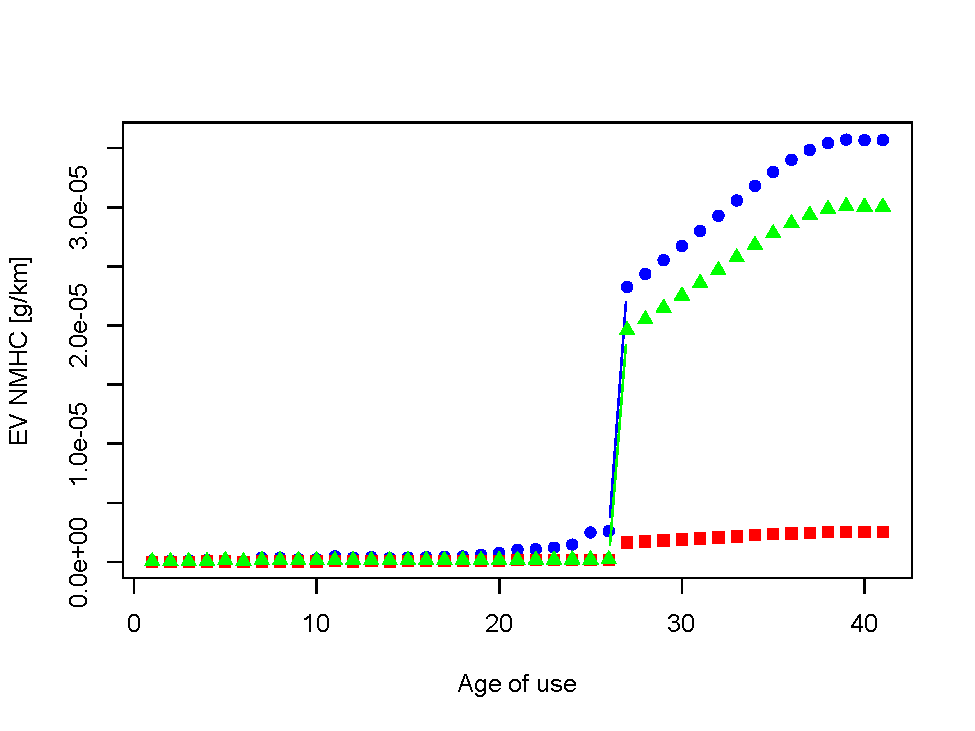
\includegraphics[width=1\linewidth]{veinbook_files/figure-latex/efEVAP-1} 

}

\caption{Hot Soak (blue), Diurnal (green) and Running Losses (red) EF (g/km)}\label{fig:efEVAP}
\end{figure}

\section{\texorpdfstring{Emission factors of wear
\texttt{ef\_wear}}{Emission factors of wear ef\_wear}}\label{emission-factors-of-wear-ef_wear}

Wear emissions are significant because they contribute with an essential
fraction of PM from the tire and brake wear. VEIN includes these
functions from \citet{NtziachristosBoulter2009} which include wearing
emission factors form tire, break and road abrasion.

The arguments are:

\begin{Shaded}
\begin{Highlighting}[]
\KeywordTok{args}\NormalTok{(ef_wear)}
\end{Highlighting}
\end{Shaded}

\begin{verbatim}
## function (wear, type, pol = "TSP", speed, load = 0.5, axle = 2) 
## NULL
\end{verbatim}

\begin{itemize}
\tightlist
\item
  \texttt{wear}: Character; type of wear: ``tyre'', ``break'' and
  ``road''
\item
  \texttt{type}: Character; type of vehicle: ``2W'', ``PC'', ``LCV'',
  'HDV"
\item
  \texttt{pol}: Character; pollutant: ``TSP'', ``PM10'', ``PM2.5'',
  ``PM1'' and ``PM0.1''
\item
  \texttt{speed}: List of speeds
\item
  \texttt{load}: Load of the HDV
\item
  \texttt{axle}: Number of axle of the HDV
\end{itemize}

\begin{Shaded}
\begin{Highlighting}[]
\KeywordTok{library}\NormalTok{(vein)}
\NormalTok{?ef_wear}
\end{Highlighting}
\end{Shaded}

\section{Emission factors from tunnel
studies}\label{emission-factors-from-tunnel-studies}

With VEIN you can choose three type of emissions factors, speed
functions, local emission factors or scaled factors. In this section, I
will show how to expand the use of local emission factors considering
tunnel emission factors \citep{perez2014emission}, from the
International Vehicle Emissions (IVE) Model \citep{Davisetal2005}
applied in Colombia \citep{gonzalez2017relative}.

\citet{perez2014emission} measured air pollutant concentrations in two
tunnels in São Paulo city, one with predominant use of LDV vehicles and
another with more HDV. The resulting emission factors for the fleet are
shown in Table \ref{tab:eftun}.

\begin{table}

\caption{\label{tab:eftun}Emission factors from tunnels in São Paulo 2014}
\centering
\begin{tabular}[t]{lrr}
\toprule
  & CO & NOx\\
\midrule
LDV & 5.8 [g/km] & 0.3 [g/km]\\
HDV & 3.6 [g/km] & 9.2 [g/km]\\
\bottomrule
\end{tabular}
\end{table}

If we want to compare these with the \citet{CETESB2015} emission
factors, we would have to weight these factors with the fleet. The
weight mean emission factor of CO and Passenger Cars (PC) is 1.40
\(g \cdot km^{-1}\) and for Light Trucks (LT) is 0.60
\(g \cdot km^{-1}\). In the case of NOx, Passenger Cars (PC) is 0.16
\(g \cdot km^{-1}\) and for Light Trucks (LT) is 3.24
\(g \cdot km^{-1}\). The emission factors from the example are for
vehicles with 0 kilometers without deterioration. Anyways, tunnel
emission factors are higher than the weighted emission factors from
CETESB.

\begin{Shaded}
\begin{Highlighting}[]
\KeywordTok{library}\NormalTok{(vein)}
\KeywordTok{data}\NormalTok{(fe2015)}
\NormalTok{fecoPC <-}\StringTok{ }\NormalTok{fe2015[fe2015}\OperatorTok{$}\NormalTok{Pollutant }\OperatorTok{==}\StringTok{ "CO"}\NormalTok{, }\StringTok{"PC_G"}\NormalTok{]}
\NormalTok{fecoLT <-}\StringTok{ }\NormalTok{fe2015[fe2015}\OperatorTok{$}\NormalTok{Pollutant }\OperatorTok{==}\StringTok{ "CO"}\NormalTok{, }\StringTok{"LT"}\NormalTok{]}
\NormalTok{fenoxPC <-}\StringTok{ }\NormalTok{fe2015[fe2015}\OperatorTok{$}\NormalTok{Pollutant }\OperatorTok{==}\StringTok{ "NOx"}\NormalTok{, }\StringTok{"PC_G"}\NormalTok{]}
\NormalTok{fenoxLT <-}\StringTok{ }\NormalTok{fe2015[fe2015}\OperatorTok{$}\NormalTok{Pollutant }\OperatorTok{==}\StringTok{ "NOx"}\NormalTok{, }\StringTok{"LT"}\NormalTok{]}
\NormalTok{PC <-}\StringTok{ }\KeywordTok{age_ldv}\NormalTok{(}\DataTypeTok{x =} \DecValTok{1}\NormalTok{, }\DataTypeTok{name =} \StringTok{"PC"}\NormalTok{, }\DataTypeTok{agemax =} \DecValTok{36}\NormalTok{, }\DataTypeTok{message =} \OtherTok{FALSE}\NormalTok{)}
\NormalTok{LT <-}\StringTok{ }\KeywordTok{age_hdv}\NormalTok{(}\DataTypeTok{x =} \DecValTok{1}\NormalTok{, }\DataTypeTok{name =} \StringTok{"LT"}\NormalTok{, }\DataTypeTok{agemax =} \DecValTok{36}\NormalTok{, }\DataTypeTok{message =} \OtherTok{FALSE}\NormalTok{)}
\KeywordTok{weighted.mean}\NormalTok{(fecoPC, PC)  }\CommentTok{# PC CO}
\end{Highlighting}
\end{Shaded}

\begin{verbatim}
## [1] 1.40355
\end{verbatim}

\begin{Shaded}
\begin{Highlighting}[]
\KeywordTok{weighted.mean}\NormalTok{(fecoLT, LT)  }\CommentTok{# LT CO}
\end{Highlighting}
\end{Shaded}

\begin{verbatim}
## [1] 0.5971173
\end{verbatim}

\begin{Shaded}
\begin{Highlighting}[]
\KeywordTok{weighted.mean}\NormalTok{(fenoxPC, PC) }\CommentTok{# PC NOx }
\end{Highlighting}
\end{Shaded}

\begin{verbatim}
## [1] 0.1699646
\end{verbatim}

\begin{Shaded}
\begin{Highlighting}[]
\KeywordTok{weighted.mean}\NormalTok{(fenoxLT, LT) }\CommentTok{# LT NOx}
\end{Highlighting}
\end{Shaded}

\begin{verbatim}
## [1] 3.241522
\end{verbatim}

If the user wants to use tunnel emission factors from
\citet{perez2014emission} in VEIN, the user would have to use the same
value for all respective categories of the vehicular composition. For
instance, after running \texttt{inventory}, include tunnel emission
factors in each \texttt{*input.R}.

\section{Emission factors from International Vehicle Emissions
(IVE)}\label{emission-factors-from-international-vehicle-emissions-ive}

The IVE model has calculated emission factors by correcting BASE
emission factors with the vehicle specific power (VSP) methodology to
predict emissions \citep{jimenez1999vehicle}. The formula is shown on
Eq. \eqref{eq:vsp}.

\begin{equation}
VSP = v \cdot (1.1 \cdot a + 9.81(atan(sin(grade))) + 0.132) + 0.000302v^3
\label{eq:vsp}
\end{equation}

where: \(v\) is velocity \((m \cdot s^{-1})\), \(a\) is the second by
second acceleration \((m \cdot s^{-2})\) and grade the second by second
change in height defined as \(\frac{(h_{t=0} - h_{t=-1})}{v}\); being
\(h\) as altitude \(m\). This method requires that the user measures the
activity Global Position System (GPS) recordings second by second and/or
emissions measurements with Portable Emissions Measurement Systems
(PEMS).

\citet{gonzalez2017relative} measure the vehicular activity in the city
of Manizales, Colombia. In this case, there were no PEMS measurements,
but IVE allows to produce emission factors from the GPS recordings based
on Mobile EPA emissions
model\citep[\citet{Davisetal2005}]{arbor2003user}.

The arguments are:

\begin{Shaded}
\begin{Highlighting}[]
\KeywordTok{args}\NormalTok{(ef_ive)}
\end{Highlighting}
\end{Shaded}

\begin{verbatim}
## function (description = "Auto/Sml Truck", fuel = "Petrol", weight = "Light", 
##     air_fuel_control = "Carburetor", exhaust = "None", evaporative = "PCV", 
##     mileage, pol, details = FALSE) 
## NULL
\end{verbatim}

\begin{itemize}
\tightlist
\item
  \texttt{description}: Character; ``Auto/Sml Truck'' ``Truck/Bus''
  or``Sml Engine''.
\item
  \texttt{fuel}: Character; ``Petrol'', ``NG Retrofit'', ``Natural
  Gas'', ``Prop Retro.'', ``Propane'', ``EthOH Retrofit'', ``OEM
  Ethanol'', ``Diesel'', ``Ethanol'' or ``CNG/LPG''.
\item
  \texttt{weight}: Character; ``Light'', ``Medium'', ``Heavy'', ``Lt'',
  ``Med'' or ``Hvy''
\item
  \texttt{air\_fuel\_control}: Character; One of the following
  characters: ``Carburetor'', ``Single-Pt FI'', ``Multi-Pt FI'',
  ``Carb/Mixer'', ``FI'', ``Pre-Chamber Inject.'', ``Direct Injection'',
  ``2-Cycle'', ``2-Cycle, FI'', ``4-Cycle, Carb'', ``4-Cycle, FI''
  ``4-Cycle''
\item
  \texttt{exhaust}: Character: ``None'', ``2-Way'', ``2-Way/EGR'',
  ``3-Way'', ``3-Way/EGR'', ``None/EGR'', ``LEV'', ``ULEV'', ``SULEV'',
  ``EuroI'', ``EuroII'', ``EuroIII'', ``EuroIV'', ``Hybrid'',
  ``Improved'', ``EGR+Improv'', ``Particulate'', ``Particulate/NOx'',
  ``EuroV'', ``High Tech'' or ``Catalyst''
\item
  \texttt{evaporative}: Character: ``PCV'', ``PCV/Tank'' or``None''.
\item
  \texttt{mileage}:Numeric; mileage of vehicle by age of use km.
\item
  \texttt{pol}: Character: ``VOC\_gkm'', ``CO\_gkm'', ``NOx\_gkm'',
  ``PM\_gkm'', ``Pb\_gkm'', ``SO2\_gkm'', ``NH3\_gkm'',
  ``ONE\_3\_butadiene\_gkm'', ``formaldehyde\_gkm'',
  ``acetaldehyde\_gkm'', ``benzene\_gkm'', ``EVAP\_gkm'', ``CO2\_gkm'',
  ``N20\_gkm'', ``CH4\_gkm'', ``VOC\_gstart'', ``CO\_gstart'',
  ``NOx\_gstart'', ``PM\_gstart'', ``Pb\_gstart'', ``SO2\_gstart'',
  ``NH3\_gstart'', ``ONE\_3butadiene\_gstart'',
  ``formaldehyde\_gstart'',``acetaldehyde\_gstart'',
  ``benzene\_gstart'', ``EVAP\_gstart'', ``CO2\_gstart'',
  ``N20\_gstart'', ``CH4\_gstart''
\item
  \texttt{details}: Logical; option to see or not more information about
  vehicle.
\end{itemize}

\section{Emission factors from the Environmental Agency of São
Paulo}\label{emission-factors-from-the-environmental-agency-of-sao-paulo}

It has been mentioned that the model includes already some emission
factors from the Environmental Agency of São Paulo CETESB for the year
2015. However, a new feature already present in VEIN is the
incorporation of all CETESB emission factors for 2016
\citep{CETESB2016}.

\begin{Shaded}
\begin{Highlighting}[]
\KeywordTok{args}\NormalTok{(ef_cetesb)}
\end{Highlighting}
\end{Shaded}

\begin{verbatim}
## function (p, veh, full = FALSE) 
## NULL
\end{verbatim}

\begin{itemize}
\tightlist
\item
  \texttt{p}: Character; Pollutants: ``COd'', ``HCd'', ``NMHCd'',
  ``CH4'', ``NOxd'', ``CO2'' ``PM'', ``N2O'', ``KML'', ``FC'', ``NO2d'',
  ``NOd'', ``gD/KWH'', ``gCO2/KWH'', ``RCHOd'', ``CO'', ``HC'',
  ``NMHC'', ``NOx'', ``NO2'' ,``NO'', ``RCHO'' (g/km). The letter `d'
  means deteriorated factor. Also, evaporative emissions at average
  temperature ranges: ``D\_20\_35'', ``S\_20\_35'', ``R\_20\_35'',
  ``D\_10\_25'', ``S\_10\_25'', ``R\_10\_25'', ``D\_0\_15'' ``S\_0\_15''
  and ``R\_0\_15'' where D means diurnal (g/day), S hot/warm soak
  (g/trip) and R hot/warm running losses (g/trip).
\item
  \texttt{veh}: Character; Vehicle categories: ``PC\_G'', ``PC\_FG'',
  ``PC\_FE'', ``PC\_E'' ``LCV\_G'', ``LCV\_FG'', ``LCV\_FE'',
  ``LCV\_E'', ``LCV\_D'', ``SLT'', ``LT'', ``MT'', ``SHT'' ``HT'',
  ``UB'', ``SUB'', ``COACH'', ``ARTIC'', ``M\_G\_150'',
  ``M\_G\_150\_500'', ``M\_G\_500'' ``M\_FG\_150'', ``M\_FG\_150\_500'',
  ``M\_FG\_500''. ``M\_FE\_150'', ``M\_FE\_150\_500'', ``M\_FE\_500'',
  ``CICLOMOTOR'', ``GNV full\\
\item
  \texttt{Logical}; To return a data.frame instead or a vector adding
  Age, Year, Brazilian emissions standards and its euro equivalents.
\end{itemize}

The letter `d' means deteriorated factor. I added the pollutants ``NO'',
``NO2'' based on the speciation of the \citet{NtziachristosSamaras2016}
guidelines.

I also added the category ``ARTIC'' for articulated buses, based on the
proportion of Articulated buses to standard urban buses on
\citet{NtziachristosSamaras2016} guidelines, which is approximately 1.4
times the standard emission factor.

\chapter{Estimation of emissions}\label{est}

The emissions estimation process was shown on Eq. \eqref{eq:emi} on
chapter \ref{ef}. In this equation, it was shown that how the emissions
are obtained by multiplying the traffic flow with the distance that each
car travels (length of the road if it is a road network), and emissions
and deterioration factors.

In this chapter, I will show how VEIN interprets this and other emission
equations to estimate emissions. At the end of each section, The Fig.
\ref{fig:diaemis} shows a diagram with the estimation process. The pink
boxes hows VEIN classes, the circle data, and the grey boxes functions.
The object \texttt{Vehicles} is a class consisting of a matrix of
vehicles with units \(1 \cdot h^{-1}\), as shown in chapter
\ref{traffic}. However, \emph{the units in \texttt{Vehicles} is not a
requirement for estimating emissions}. The object of class
\texttt{Speed} is a matrix of speeds with the number of columns as the
calculated speeds at different hours at each row. This object can be
present or not, depending on the type of emission factor considered, for
an instant, emission factors not depending on speed. The object class of
\texttt{EmissionFactorsList} are a list of functions depending on speed
as \(f(V)\). Each function can depend on speed or not as shown in
chapter \ref{ef}, section \ref{localef}. Lastly, the object lkm is the
length of the road expressed in \(lkm\).

The function \texttt{emis} reads the inputs and estimates the emissions
producing an object with class \texttt{EmissionsArray} which has 4
dimensions, number of streets, ages of use of a vehicle, number of hours
and number of days.

\begin{figure}

{\centering 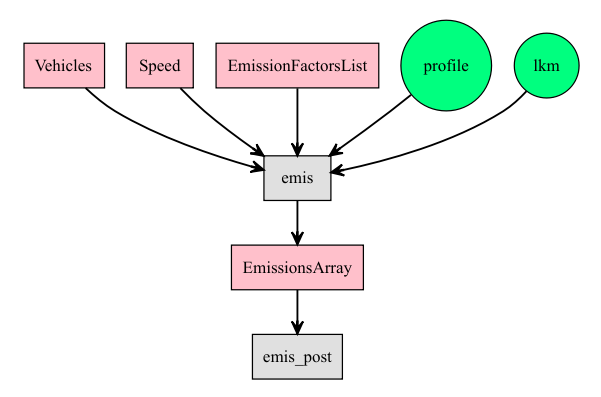
\includegraphics[width=0.8\linewidth]{figuras/dia6} 

}

\caption{Emissions estimation process with VEIN}\label{fig:diaemis}
\end{figure}

The estimation process is done with the emissions functions. The
emissions estimations functions are:

\begin{itemize}
\tightlist
\item
  \texttt{emis} for hot emissions,
\item
  \texttt{emis\_cold} for cold start emissions,
\item
  \texttt{emis\_evap} for evaporative emissions,
\item
  \texttt{emis\_paved} for resuspension emissions on paved roads, and
\item
  \texttt{emis\_wear} for wear of brakes, tyres, and roads.
\end{itemize}

These functions perform internal checks for ensuring that the length lkm
has the unit of \(km\). This means that, if \texttt{lkm} has units
different than \(km\), the function will not run. These function runs
internally \texttt{lapply} which are faster \texttt{for} written in C.
Despite that these functions are fast, i will try to make them faster
with some RCPP implementation in the future.

\section{\texorpdfstring{The \texttt{emis}
function}{The emis function}}\label{the-emis-function}

The arguments of \texttt{emis} are:

\begin{Shaded}
\begin{Highlighting}[]
\KeywordTok{args}\NormalTok{(vein}\OperatorTok{::}\NormalTok{emis)}
\end{Highlighting}
\end{Shaded}

\begin{verbatim}
## function (veh, lkm, ef, speed = 34, agemax = ifelse(is.data.frame(veh), 
##     ncol(veh), ncol(veh[[1]])), profile, hour = nrow(profile), 
##     day = ncol(profile), array = T, verbose = FALSE) 
## NULL
\end{verbatim}

\begin{itemize}
\tightlist
\item
  \texttt{veh}: ``Vehicles'' data-frame or list of ``Vehicles''
  data-frame. Each data-frame has some columns matching the age
  distribution of that type of vehicle. The number of rows is equal to
  the number of streets link.
\item
  \texttt{lkm}: Length of each link that must in \(km\). As consequence,
  emission factors must be in \(g \cdot km^{-1}\).
\item
  \texttt{ef}: ``EmissionFactorsList''. A list of emission factors as
  speed functions. Each element has the form \(f(V)\). The implicit unit
  is \(g \cdot km^{-1}\).
\item
  \texttt{speed}: ``Speed'' object. A Speed data-frame with some columns
  as hours.
\item
  \texttt{agemax}: Age of oldest vehicles of the vehicles veh. The
  information of this argument can be obtained from the \texttt{veh}
  argument. Therefore, this argument will be deprecated.
\item
  \texttt{profile}: Numerical or dataframe or matrix with nrows equal to
  the hours and cols to each day. This is traffic data normalized to the
  hour of the input traffic data.
\item
  \texttt{hour}: Number of considered hours in estimation. As this
  information can be derived from the argument \texttt{profile}, the
  default value is the number of rows of the matrix profile.
\item
  \texttt{day}: Number of considered days in estimation. As this
  information can be derived from the argument \texttt{profile}, the
  default value is the number of columns of the matrix profile.
\item
  \texttt{array}: When FALSE produces a dataframe of the estimation.
  When TRUE expects a profile as a dataframe producing an array with
  dimensions (streets x columns x hours x days)
\end{itemize}

When the only arguments present in the function are \textbf{veh},
\textbf{lkm} and \textbf{ef} assumes a \emph{top-down} and shows a
message.

\section{\texorpdfstring{The \texttt{emis\_cold}
function}{The emis\_cold function}}\label{the-emis_cold-function}

The arguments of \texttt{emis\_cold} are:

\begin{Shaded}
\begin{Highlighting}[]
\KeywordTok{args}\NormalTok{(vein}\OperatorTok{::}\NormalTok{emis_cold)}
\end{Highlighting}
\end{Shaded}

\begin{verbatim}
## function (veh, lkm, ef, efcold, beta, speed = 34, agemax = if (!inherits(x = veh, 
##     what = "list")) {
##     ncol(veh)
## } else {
##     ncol(veh[[1]])
## }, profile, hour = nrow(profile), day = ncol(profile), array = TRUE) 
## NULL
\end{verbatim}

The arguments are similar to \texttt{emis} with the difference that it
is added two arguments:

\begin{itemize}
\tightlist
\item
  \texttt{cold}: List of functions of cold start emission factors of
  vehicular categories. Technically, each function is also of the form
  \(f(V)\).
\item
  \texttt{beta}: Datraframe with the hourly cold-start distribution to
  each day of the period. Some rows are hours and columns are days. It
  represents the fraction of mileage driven under cold-start conditions.
\end{itemize}

The equation for estimating cold-start emissions is on Eq.
\eqref{eq:cold}.

\section{\texorpdfstring{The \texttt{emis\_evap}
function}{The emis\_evap function}}\label{the-emis_evap-function}

The estimation of evaporative emissions applies Tier 2 from
\citet{MelliosNtziachristos2016}. The approach followed in VEIN was very
merely, consisting in only adding elements of a data-frame.

\begin{Shaded}
\begin{Highlighting}[]
\KeywordTok{args}\NormalTok{(vein}\OperatorTok{::}\NormalTok{emis_evap)}
\end{Highlighting}
\end{Shaded}

\begin{verbatim}
## function (veh, name, size, fuel, aged, nd4, nd3, nd2, nd1, hs_nd4, 
##     hs_nd3, hs_nd2, hs_nd1, rl_nd4, rl_nd3, rl_nd2, rl_nd1, d_nd4, 
##     d_nd3, d_nd2, d_nd1) 
## NULL
\end{verbatim}

\begin{itemize}
\tightlist
\item
  \texttt{veh}: this is the number of vehicles at each age of use and
  for each street. It is a \texttt{Vehicles} object.
\item
  \texttt{name}: Character indicating the name of the vehicle.
\item
  \texttt{size}: Character indicating the size of the vehicle.
\item
  \texttt{fuel}: Character indicating the fuel of the vehicle.
\item
  \texttt{age}: Numeric vector with the age distribution, for instance,
  1:40 for vehicles between 1 and 40 years of use.
\item
  \texttt{nd4}: Number of days of your period of study with monthly
  average Temperature between 20 and 35 Celsius degrees. If the period
  is a year, this is the annual number of days under that condition.
\item
  \texttt{nd3}: Number of days of your period of study with a monthly
  average temperature between 10 and 25 Celsius degrees.
\item
  \texttt{nd2}: Number of days of your period of study with a monthly
  average temperature between 0 and 15 Celcius degrees.
\item
  \texttt{nd1}: Number of days of your period of study with a monthly
  average temperature between -5 and 10 Celsius degrees.
\item
  \texttt{hs\_nd4}: Number of average daily hot-soak evaporative
  emissions for days with temperature between 20 and 35 Celcius degrees
\item
  \texttt{hs\_nd3}: Number of average daily hot-soak evaporative
  emissions for days with temperature between 10 and 25 Celcius degrees
\item
  \texttt{hs\_nd2}: Number of average daily hot-soak evaporative
  emissions for days with temperature between 0 and 15 Celcius degrees
\item
  \texttt{hs\_nd1}: Number of average daily hot-soak evaporative
  emissions for days with temperature between -5 and 10 Celcius degrees
\item
  \texttt{rl\_nd4}: Number of average daily running losses evaporative
  emissions for days with a temperature between 20 and 35 Celcius
  degrees
\item
  \texttt{rl\_nd3}: Number of average daily running losses evaporative
  emissions for days with a temperature between 10 and 25 Celcius
  degrees
\item
  \texttt{rl\_nd2}: Number of average daily running losses evaporative
  emissions for days with a temperature between 0 and 15 Celcius degrees
\item
  \texttt{rl\_nd1}: Number of average daily running losses evaporative
  emissions for days with a temperature between -5 and 10 Celcius
  degrees
\item
  \texttt{d\_nd4}: Number of average daily diurnal evaporative emissions
  for days with temperature between 20 and 35 Celcius degrees
\item
  \texttt{d\_nd3}: Number of average daily diurnal evaporative emissions
  for days with temperature between 10 and 25 Celcius degrees
\item
  \texttt{d\_nd2}: Number of average daily diurnal evaporative emissions
  for days with temperature between 0 and 15 Celcius degrees
\item
  \texttt{d\_nd1}: Number of average daily diurnal evaporative emissions
  for days with temperature between -5 and 10 Celcius degrees
\end{itemize}

\section{\texorpdfstring{The \texttt{emis\_paved}
function}{The emis\_paved function}}\label{the-emis_paved-function}

Evaporative emissions are emissions of resuspended dust due to traffic
circulating over paved or non-paved roads. These emissions can be a
vital source of mass particulate matter and several cities programs that
aim to improve air quality by diminishing these emissions
\citep{AMATO20103070}. However, these emissions are not considered by in
the European emissions guidelines, where their focus is on primary
particles and not those resulting from the resuspension of previously
deposited material \citep{NtziachristosBoulter2009}.

The method adopted in VEIN comes from the USEPA \citep{paved} which
presents equations for annual, daily and hourly estimations:

\begin{equation}
EF_{paved}=k \cdot sL^{0.91} \cdot W^{1.02}
\label{eq:res1}
\end{equation}

Where

\begin{itemize}
\tightlist
\item
  \(EF_{paved}\) is the emission factor of particulate matter.
\item
  \(k\) particle size splitter.
\item
  \(sL\) road surface silt loading \(g \cdot m^{-2}\).
\item
  \(W\) average weight.
\end{itemize}

Equation \eqref{eq:res1} can be extrapolated to consider natural
mitigation of rainy periods of time with daily basis:

\begin{equation}
EF_{anual} = EF_{paved} \cdot (1 - \frac{P}{4 \cdot N})
\label{eq:res2}
\end{equation}

Where

\begin{itemize}
\tightlist
\item
  \(EF_{anual}\) annual or long-term emission factor.
\item
  \(P\) number of days with accumulated rain above 0.254 mm.
\item
  \(N\) total number of days.
\end{itemize}

alternatively, hourly

\begin{equation}
EF_{hourly} = EF_{paved} \cdot (1 - \frac{1.2 \cdot P}{N})
\label{eq:res2}
\end{equation}

Where

\begin{itemize}
\tightlist
\item
  \(EF_{annual}\) annual or long-term emission factor.
\item
  \(P\) number of hours with accumulated rain above 0.254 mm.
\item
  \(N\) total number of hours. For instance, 8760 for 1 year.
\end{itemize}

The function \texttt{emis\_paved} has the arguments:

\begin{Shaded}
\begin{Highlighting}[]
\KeywordTok{args}\NormalTok{(vein}\OperatorTok{::}\NormalTok{emis_paved)}
\end{Highlighting}
\end{Shaded}

\begin{verbatim}
## function (veh, lkm, k = 0.62, sL1 = 0.6, sL2 = 0.2, sL3 = 0.06, 
##     sL4 = 0.03, W) 
## NULL
\end{verbatim}

Where,

-\texttt{veh}: It is an array with dimenssions number of streets x hours
of day x days of week. - \texttt{lkm}: Length of each link. -
\texttt{k}: K\_PM30 = 3.23, K\_PM15 = 0.77, K\_PM10 = 0.62 and K\_PM2.5
= 0.15. - \texttt{sL1}: Silt loading (g/m2) for roads with ADT
\textless{}= 500. - \texttt{sL2}: Silt loading (g/m2) for roads with ADT
\textgreater{} 500 and \textless{}= 5000. - \texttt{sL3}: Silt loading
(g/m2) for roads with ADT \textgreater{} 5000 and \textless{}= 1000. -
\texttt{sL4}: Silt loading (g/m2) for roads with ADT \textgreater{}
10000. - \texttt{W}: array of dimensions of veh. It consists in the
hourly averaged weight of traffic fleet in each road.

For instance, Let's create an array of vehicles. The function
\texttt{adt} calculates the number of vehicles at all hours. Let's use
the \texttt{data(net)} assuming no buses. Let's calculate the total
traffic for only 24 hours with the same profile. For Simplicity, let's
assume that all vehicle are expressed in \emph{vehicle equivalent}
Moreover, it is a dry period.

\begin{Shaded}
\begin{Highlighting}[]
\KeywordTok{library}\NormalTok{(vein)}
\KeywordTok{data}\NormalTok{(net)}
\KeywordTok{data}\NormalTok{(profiles)}
\NormalTok{vkpc  <-}\StringTok{ }\KeywordTok{vkm}\NormalTok{(net}\OperatorTok{$}\NormalTok{ldv}\OperatorTok{*}\FloatTok{0.75}\NormalTok{, }\DecValTok{1}\NormalTok{, }\KeywordTok{matrix}\NormalTok{(profiles}\OperatorTok{$}\NormalTok{PC_JUNE_}\DecValTok{2012}\NormalTok{[, }\DecValTok{1}\NormalTok{]))}
\NormalTok{vklcv  <-}\StringTok{ }\KeywordTok{vkm}\NormalTok{(net}\OperatorTok{$}\NormalTok{ldv}\OperatorTok{*}\FloatTok{0.1}\NormalTok{, }\DecValTok{1}\NormalTok{, }\KeywordTok{matrix}\NormalTok{(profiles}\OperatorTok{$}\NormalTok{LCV_JUNE_}\DecValTok{2012}\NormalTok{[, }\DecValTok{1}\NormalTok{]))}
\NormalTok{vkmc  <-}\StringTok{ }\KeywordTok{vkm}\NormalTok{(net}\OperatorTok{$}\NormalTok{ldv}\OperatorTok{*}\FloatTok{0.15}\NormalTok{, }\DecValTok{1}\NormalTok{, }\KeywordTok{matrix}\NormalTok{(profiles}\OperatorTok{$}\NormalTok{MC_JUNE_}\DecValTok{2012}\NormalTok{[, }\DecValTok{1}\NormalTok{]))}
\NormalTok{vkhgv  <-}\StringTok{ }\KeywordTok{vkm}\NormalTok{(net}\OperatorTok{$}\NormalTok{hdv, }\DecValTok{1}\NormalTok{, }\KeywordTok{matrix}\NormalTok{(profiles}\OperatorTok{$}\NormalTok{HGV_JUNE_}\DecValTok{2012}\NormalTok{[, }\DecValTok{1}\NormalTok{]))}
\NormalTok{vk <-}\StringTok{ }\NormalTok{vkpc }\OperatorTok{+}\StringTok{ }\NormalTok{vklcv }\OperatorTok{+}\StringTok{ }\NormalTok{vkmc }\OperatorTok{+}\StringTok{ }\NormalTok{vkhgv}
\KeywordTok{dim}\NormalTok{(vk)}
\end{Highlighting}
\end{Shaded}

\begin{verbatim}
## [1] 1505   24
\end{verbatim}

\texttt{W} is the average hourly fleet weight. It has the same
dimensions of \texttt{adt2}. Let's assume an individual weight of PC is
1, LCV 1.5, HGV = 10 and MC 0.5. This example is a simplification,
\texttt{adt} should be calculated with a full characterization of the
fleet.

\begin{Shaded}
\begin{Highlighting}[]
\NormalTok{wpc  <-}\StringTok{ }\KeywordTok{vkm}\NormalTok{(net}\OperatorTok{$}\NormalTok{ldv}\OperatorTok{*}\FloatTok{0.75}\NormalTok{, }\DecValTok{1}\NormalTok{, profiles}\OperatorTok{$}\NormalTok{PC_JUNE_}\DecValTok{2012}\NormalTok{[, }\DecValTok{1}\NormalTok{])}\OperatorTok{*}\DecValTok{1}
\NormalTok{wlcv  <-}\StringTok{ }\KeywordTok{vkm}\NormalTok{(net}\OperatorTok{$}\NormalTok{ldv}\OperatorTok{*}\FloatTok{0.1}\NormalTok{, }\DecValTok{1}\NormalTok{, profiles}\OperatorTok{$}\NormalTok{LCV_JUNE_}\DecValTok{2012}\NormalTok{[, }\DecValTok{1}\NormalTok{])}\OperatorTok{*}\FloatTok{1.5}
\NormalTok{wmc  <-}\StringTok{ }\KeywordTok{vkm}\NormalTok{(net}\OperatorTok{$}\NormalTok{ldv}\OperatorTok{*}\FloatTok{0.15}\NormalTok{, }\DecValTok{1}\NormalTok{, profiles}\OperatorTok{$}\NormalTok{MC_JUNE_}\DecValTok{2012}\NormalTok{[, }\DecValTok{1}\NormalTok{])}\OperatorTok{*}\FloatTok{0.5}
\NormalTok{whgv  <-}\StringTok{ }\KeywordTok{vkm}\NormalTok{(net}\OperatorTok{$}\NormalTok{hdv, }\DecValTok{1}\NormalTok{, profiles}\OperatorTok{$}\NormalTok{HGV_JUNE_}\DecValTok{2012}\NormalTok{[, }\DecValTok{1}\NormalTok{])}\OperatorTok{*}\DecValTok{10}
\NormalTok{W <-}\StringTok{ }\NormalTok{(wpc }\OperatorTok{+}\StringTok{ }\NormalTok{wlcv }\OperatorTok{+}\StringTok{ }\NormalTok{wmc }\OperatorTok{+}\StringTok{ }\NormalTok{whgv)}\OperatorTok{/}\NormalTok{vk}
\NormalTok{W[}\KeywordTok{is.na}\NormalTok{(W)] <-}\StringTok{ }\DecValTok{0}
\KeywordTok{dim}\NormalTok{(W)}
\end{Highlighting}
\end{Shaded}

\begin{verbatim}
## [1] 1505   24
\end{verbatim}

moreover, now we estimate the emissions with the default values form
PM10.

\begin{Shaded}
\begin{Highlighting}[]
\NormalTok{emi <-}\StringTok{ }\KeywordTok{emis_paved}\NormalTok{(}\DataTypeTok{veh =}\NormalTok{ vk, }\DataTypeTok{lkm =}\NormalTok{ net}\OperatorTok{$}\NormalTok{lkm, }\DataTypeTok{W =}\NormalTok{ W)}
\NormalTok{emi[}\DecValTok{1}\OperatorTok{:}\DecValTok{4}\NormalTok{, }\DecValTok{1}\OperatorTok{:}\DecValTok{4}\NormalTok{]}
\end{Highlighting}
\end{Shaded}

\begin{verbatim}
## Result for Emissions 
##                h1              h2              h3              h4
## 1 28.492378 [g/h] 41.326236 [g/h] 27.987685 [g/h] 30.978253 [g/h]
## 2 48.704190 [g/h] 31.257192 [g/h] 27.139666 [g/h] 34.919757 [g/h]
## 3  4.360828 [g/h]  2.327479 [g/h]  1.576257 [g/h]  1.744684 [g/h]
## 4 10.371056 [g/h]  5.535283 [g/h]  3.748702 [g/h]  4.149262 [g/h]
\end{verbatim}

\section{\texorpdfstring{The \texttt{emis\_wear}
function}{The emis\_wear function}}\label{ew}

Wear emissions can be very important these are a second most important
source of particulate matter in Europe \citep{eear}. These methods in
VEIN comes from \citet{NtziachristosBoulter2009} which include wear of
``tire'', ``break'' and ``road''.

The arguments of the function \texttt{emis\_wear} are:

\begin{Shaded}
\begin{Highlighting}[]
\KeywordTok{args}\NormalTok{(vein}\OperatorTok{::}\NormalTok{emis_wear)}
\end{Highlighting}
\end{Shaded}

\begin{verbatim}
## function (veh, lkm, ef, what = "tyre", speed, agemax = ncol(veh), 
##     profile, hour = nrow(profile), day = ncol(profile)) 
## NULL
\end{verbatim}

Where,

\begin{itemize}
\tightlist
\item
  \texttt{veh}: Object of class ``Vehicles''.
\item
  \texttt{lkm}: Length of the road.
\item
  \texttt{ef}: list of emission factor functions class
  ``EmissionFactorsList'', length equals to hours.
\item
  \texttt{agemax}: Age of oldest vehicles for that category
\item
  \texttt{profile}: Dataframe or matrix with nrows equal to hours and
  number of columns col as days of the week
\item
  \texttt{hour}: Number of considered hours in estimation, with default
  value as some rows of the profile.
\item
  \texttt{day}: Number of considered days in estimation, with default
  value as some columns of the profile.
\end{itemize}

Let's estimate wear emissions!

First, we get the emission factor with the \texttt{ef\_wear} function:

\begin{Shaded}
\begin{Highlighting}[]
\KeywordTok{library}\NormalTok{(vein)}
\KeywordTok{data}\NormalTok{(net)}
\KeywordTok{data}\NormalTok{(profiles)}
\NormalTok{pro <-}\StringTok{ }\NormalTok{profiles}\OperatorTok{$}\NormalTok{PC_JUNE_}\DecValTok{2012}\NormalTok{[, }\DecValTok{1}\NormalTok{] }\CommentTok{# 24 hours}
\NormalTok{pc_week <-}\StringTok{ }\KeywordTok{temp_fact}\NormalTok{(net}\OperatorTok{$}\NormalTok{ldv}\OperatorTok{+}\NormalTok{net}\OperatorTok{$}\NormalTok{hdv, pro)}
\NormalTok{df <-}\StringTok{ }\KeywordTok{netspeed}\NormalTok{(pc_week, net}\OperatorTok{$}\NormalTok{ps, net}\OperatorTok{$}\NormalTok{ffs, net}\OperatorTok{$}\NormalTok{capacity, net}\OperatorTok{$}\NormalTok{lkm, }\DataTypeTok{alpha =} \DecValTok{1}\NormalTok{)}
\NormalTok{ef <-}\StringTok{ }\KeywordTok{ef_wear}\NormalTok{(}\DataTypeTok{wear =} \StringTok{"tyre"}\NormalTok{, }\DataTypeTok{type =} \StringTok{"PC"}\NormalTok{, }\DataTypeTok{pol =} \StringTok{"PM10"}\NormalTok{, }
                            \DataTypeTok{speed =}\NormalTok{ df)}
\end{Highlighting}
\end{Shaded}

Then we estimate emissions

\begin{Shaded}
\begin{Highlighting}[]
\NormalTok{emi <-}\StringTok{ }\KeywordTok{emis_wear}\NormalTok{(}\DataTypeTok{veh =} \KeywordTok{age_ldv}\NormalTok{(net}\OperatorTok{$}\NormalTok{ldv, }\DataTypeTok{name =} \StringTok{"VEH"}\NormalTok{), }\DataTypeTok{speed =}\NormalTok{ df,}
                 \DataTypeTok{lkm =}\NormalTok{ net}\OperatorTok{$}\NormalTok{lkm, }\DataTypeTok{ef =}\NormalTok{ ef, }\DataTypeTok{profile =}\NormalTok{  pro)}
\end{Highlighting}
\end{Shaded}

\begin{verbatim}
## Average age of VEH is 11.17
\end{verbatim}

\begin{verbatim}
## Number of VEH is 1946.95 * 10^3 veh
\end{verbatim}

\begin{Shaded}
\begin{Highlighting}[]
\NormalTok{df <-}\StringTok{ }\KeywordTok{emis_post}\NormalTok{(emi, }\DataTypeTok{pollutant =} \StringTok{"PM"}\NormalTok{, }\DataTypeTok{by =} \StringTok{"streets_wide"}\NormalTok{)}
\NormalTok{df[}\DecValTok{1}\OperatorTok{:}\DecValTok{4}\NormalTok{, }\DecValTok{1}\OperatorTok{:}\DecValTok{4}\NormalTok{]}
\end{Highlighting}
\end{Shaded}

\begin{verbatim}
## Result for Emissions 
##                V1              V2               V3               V4
## 1 2.0689049 [g/h] 1.0160833 [g/h] 0.56468672 [g/h] 0.52486176 [g/h]
## 2 0.7614073 [g/h] 0.3743085 [g/h] 0.20803274 [g/h] 0.19336135 [g/h]
## 3 0.1116298 [g/h] 0.0548773 [g/h] 0.03049965 [g/h] 0.02834868 [g/h]
## 4 0.2768287 [g/h] 0.1360872 [g/h] 0.07563435 [g/h] 0.07030028 [g/h]
\end{verbatim}

\chapter{\texorpdfstring{Post estimation with
\texttt{emis\_post}}{Post estimation with emis\_post}}\label{post}

Once the emissions are estimated we obtained \texttt{EmissionsArray}
objects, which as mentioned before, they are arrays with the dimensions
streets x age distribution of vehicles x hours x days.

\begin{figure}

{\centering 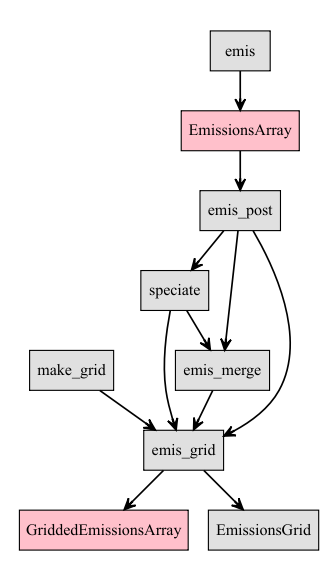
\includegraphics[width=1\linewidth]{figuras/dia7} 

}

\caption{Post-emissions}\label{fig:demispost}
\end{figure}

Now the function \texttt{emis\_post} reads the \texttt{EmissionsArray}
and and convert it to data-frames that are easier to manage.

The arguments of \texttt{emis\_post} are:

\begin{Shaded}
\begin{Highlighting}[]
\KeywordTok{args}\NormalTok{(vein}\OperatorTok{::}\NormalTok{emis_post)}
\end{Highlighting}
\end{Shaded}

\begin{verbatim}
## function (arra, veh, size, fuel, pollutant, by = "veh", net) 
## NULL
\end{verbatim}

Where,

\begin{itemize}
\tightlist
\item
  \texttt{arra}: \texttt{EmissionsArray} obtained with the \texttt{emis}
  functions. It is an array of emissions 4d: streets x category of
  vehicles x hours x days or 3d: streets x category of vehicles x hours
\item
  \texttt{veh}: Character indicating the type of vehicle , for instance:
  ``PC''.
\item
  \texttt{size}: Character indicating the size or weight, for instance:
  ``\textless{}1400'', ``1400\textless{}cc\textless{}2000'', ``GLP'',
  ``Diesel''.
\item
  \texttt{fuel}: Character indicating fuel, for instance: ``Gasoline'',
  ``E\_25'', ``GLP'', ``Diesel''.
\item
  \texttt{pollutant}: Character indicating the pollutant, for instance
  ``CO'', ``NOx'', etc.
\item
  \texttt{by}: Character indicating type of output, ``veh'' for total
  vehicular category , ``streets\_narrow'' or ``streets\_wide''. This is
  the most important argument of this function. ``streets\_wide''
  returns a dataframe with rows as number of streets and columns the
  hours as days*hours considered, e.g.~168 columns as the hours of a
  whole week and ``streets\_wide repeats the row number of streets by
  hour and day of the week
\end{itemize}

Lets create some objects

\section{Emissions by street}\label{emissions-by-street}

From previous chapters we worked with \texttt{Vehicles},
\texttt{EmissionFactors} and estimate emissions generating
\texttt{EmissionsArray}. Now let's create an \texttt{EmissionsArray}
object.

\begin{Shaded}
\begin{Highlighting}[]
\KeywordTok{library}\NormalTok{(vein)}
\KeywordTok{library}\NormalTok{(veinreport)}
\KeywordTok{library}\NormalTok{(cptcity)}
\KeywordTok{library}\NormalTok{(ggplot2)}
\KeywordTok{data}\NormalTok{(net)}
\KeywordTok{data}\NormalTok{(profiles)}
\KeywordTok{data}\NormalTok{(fe2015)}
\NormalTok{PC_G <-}\StringTok{ }\KeywordTok{age_ldv}\NormalTok{(}\DataTypeTok{x =}\NormalTok{ net}\OperatorTok{$}\NormalTok{ldv, }\DataTypeTok{name =} \StringTok{"PC"}\NormalTok{)}
\end{Highlighting}
\end{Shaded}

\begin{verbatim}
## Average age of PC is 11.17
\end{verbatim}

\begin{verbatim}
## Number of PC is 1946.95 * 10^3 veh
\end{verbatim}

\begin{Shaded}
\begin{Highlighting}[]
\CommentTok{# Estimation for 168 hour and local factors}
\NormalTok{pcw <-}\StringTok{ }\KeywordTok{temp_fact}\NormalTok{(net}\OperatorTok{$}\NormalTok{ldv, profiles}\OperatorTok{$}\NormalTok{PC_JUNE_}\DecValTok{2014}\NormalTok{)}
\CommentTok{# June is not holliday in southern hemisphere}
\NormalTok{hdvw <-}\StringTok{ }\KeywordTok{temp_fact}\NormalTok{(net}\OperatorTok{$}\NormalTok{hdv, profiles}\OperatorTok{$}\NormalTok{HGV_JUNE_}\DecValTok{2014}\NormalTok{)}
\NormalTok{speed <-}\StringTok{ }\KeywordTok{netspeed}\NormalTok{(pcw }\OperatorTok{+}\StringTok{ }\NormalTok{hdvw, net}\OperatorTok{$}\NormalTok{ps, net}\OperatorTok{$}\NormalTok{ffs, net}\OperatorTok{$}\NormalTok{capacity, net}\OperatorTok{$}\NormalTok{lkm, }\DataTypeTok{alpha =} \DecValTok{1}\NormalTok{)}
\NormalTok{lef <-}\StringTok{ }\KeywordTok{EmissionFactorsList}\NormalTok{(fe2015[fe2015}\OperatorTok{$}\NormalTok{Pollutant}\OperatorTok{==}\StringTok{"CO"}\NormalTok{, }\StringTok{"PC_G"}\NormalTok{])}
\NormalTok{E_CO <-}\StringTok{ }\KeywordTok{emis}\NormalTok{(}\DataTypeTok{veh =}\NormalTok{ PC_G,}\DataTypeTok{lkm =}\NormalTok{ net}\OperatorTok{$}\NormalTok{lkm, }\DataTypeTok{ef =}\NormalTok{ lef, }\DataTypeTok{speed =}\NormalTok{ speed,}
             \DataTypeTok{profile =}\NormalTok{ profiles}\OperatorTok{$}\NormalTok{PC_JUNE_}\DecValTok{2014}\NormalTok{)}
\end{Highlighting}
\end{Shaded}

\begin{verbatim}
## 187546.38 kg emissions in 24 hours and 7 days
\end{verbatim}

Now that we have our \texttt{EmissionsArray} E\_CO, we can process it
with the function \texttt{emis\_post}. The emissions by street are
obtained with the argument \texttt{by} = ``streets\_wide'':

\begin{Shaded}
\begin{Highlighting}[]
\NormalTok{E_CO_STREETS <-}\StringTok{ }\KeywordTok{emis_post}\NormalTok{(E_CO, }\DataTypeTok{by =} \StringTok{"streets_wide"}\NormalTok{)}
\NormalTok{E_CO_STREETS[}\DecValTok{1}\OperatorTok{:}\DecValTok{6}\NormalTok{, }\DecValTok{1}\OperatorTok{:}\DecValTok{3}\NormalTok{]}
\end{Highlighting}
\end{Shaded}

\begin{verbatim}
## Result for Emissions 
##                 V1               V2              V3
## 1 676.629408 [g/h] 349.068278 [g/h] 206.13032 [g/h]
## 2 259.924802 [g/h] 134.093349 [g/h]  79.18423 [g/h]
## 3  38.107534 [g/h]  19.659404 [g/h]  11.60919 [g/h]
## 4  90.628506 [g/h]  46.754599 [g/h]  27.60933 [g/h]
## 5   3.884417 [g/h]   2.003943 [g/h]   1.18336 [g/h]
## 6 378.775340 [g/h] 195.407492 [g/h] 115.39120 [g/h]
\end{verbatim}

In the version 0.3.17 it was added the capability of returning an
spatial object class `sf' with `LINESTRING':

\begin{Shaded}
\begin{Highlighting}[]
\NormalTok{E_CO_STREETS <-}\StringTok{ }\KeywordTok{emis_post}\NormalTok{(E_CO, }\DataTypeTok{by =} \StringTok{"streets_wide"}\NormalTok{, }\DataTypeTok{net =}\NormalTok{ net)}
\KeywordTok{class}\NormalTok{(E_CO_STREETS)}
\end{Highlighting}
\end{Shaded}

\begin{verbatim}
## [1] "sf"         "data.frame"
\end{verbatim}

\begin{Shaded}
\begin{Highlighting}[]
\KeywordTok{ggplot}\NormalTok{(E_CO_STREETS) }\OperatorTok{+}\StringTok{ }\KeywordTok{geom_sf}\NormalTok{(}\KeywordTok{aes}\NormalTok{(}\DataTypeTok{colour =} \KeywordTok{as.numeric}\NormalTok{(V9))) }\OperatorTok{+}
\StringTok{  }\KeywordTok{scale_color_gradientn}\NormalTok{(}\DataTypeTok{colours =} \KeywordTok{rev}\NormalTok{(}\KeywordTok{cpt}\NormalTok{())) }\OperatorTok{+}\StringTok{ }\KeywordTok{theme_bw}\NormalTok{()}\OperatorTok{+}
\StringTok{  }\KeywordTok{ggtitle}\NormalTok{(}\StringTok{"CO emissions at 08:00 (g/h)"}\NormalTok{)}
\end{Highlighting}
\end{Shaded}

\begin{figure}
\centering
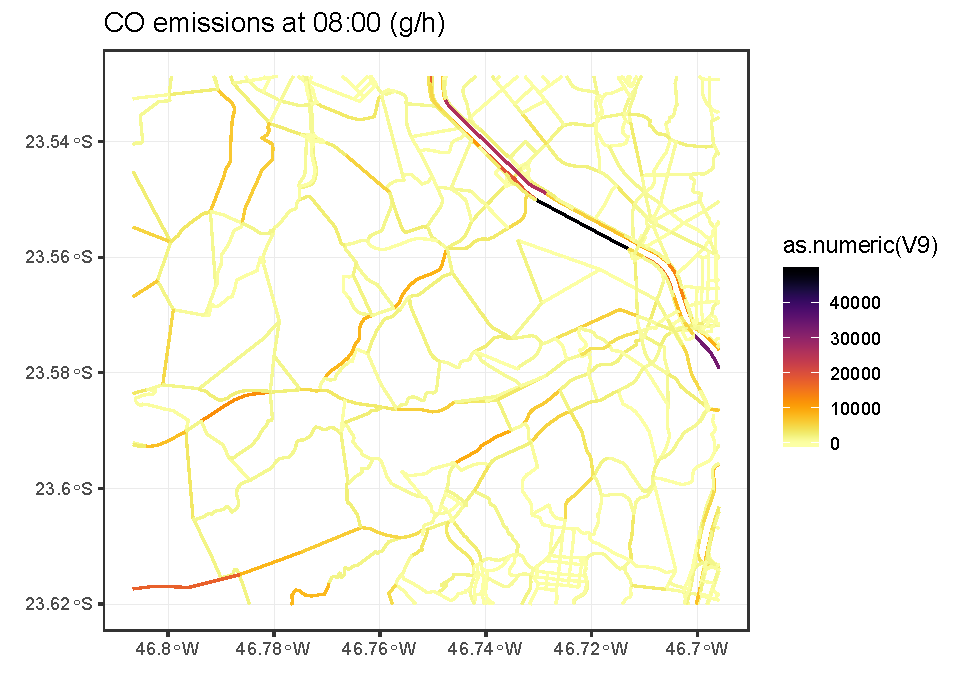
\includegraphics{veinbook_files/figure-latex/pcco-1.pdf}
\caption{\label{fig:pcco}CO emisions of PC (g/h)}
\end{figure}

Now, if we estimate the NOx emissions of Light Trucks we will a slight
different pattern of emissions:

\begin{Shaded}
\begin{Highlighting}[]
\NormalTok{LT <-}\StringTok{ }\KeywordTok{age_hdv}\NormalTok{(}\DataTypeTok{x =}\NormalTok{ net}\OperatorTok{$}\NormalTok{hdv, }\DataTypeTok{name =} \StringTok{"LT"}\NormalTok{)}
\end{Highlighting}
\end{Shaded}

\begin{verbatim}
## Average age of LT is 17.12
\end{verbatim}

\begin{verbatim}
## Number of LT is 148.12 * 10^3 veh
\end{verbatim}

\begin{Shaded}
\begin{Highlighting}[]
\NormalTok{lef <-}\StringTok{ }\KeywordTok{EmissionFactorsList}\NormalTok{(fe2015[fe2015}\OperatorTok{$}\NormalTok{Pollutant}\OperatorTok{==}\StringTok{"NOx"}\NormalTok{, }\StringTok{"LT"}\NormalTok{])}
\NormalTok{E_NOx <-}\StringTok{ }\KeywordTok{emis}\NormalTok{(}\DataTypeTok{veh =}\NormalTok{ LT, }\DataTypeTok{lkm =}\NormalTok{ net}\OperatorTok{$}\NormalTok{lkm, }\DataTypeTok{ef =}\NormalTok{ lef, }\DataTypeTok{speed =}\NormalTok{ speed,}
              \DataTypeTok{profile =}\NormalTok{ profiles}\OperatorTok{$}\NormalTok{PC_JUNE_}\DecValTok{2014}\NormalTok{)}
\end{Highlighting}
\end{Shaded}

\begin{verbatim}
## 34029.87 kg emissions in 24 hours and 7 days
\end{verbatim}

\begin{Shaded}
\begin{Highlighting}[]
\NormalTok{E_NOx_STREETS <-}\StringTok{ }\KeywordTok{emis_post}\NormalTok{(E_NOx, }\DataTypeTok{by =} \StringTok{"streets_wide"}\NormalTok{, }\DataTypeTok{net =}\NormalTok{ net)}
\KeywordTok{ggplot}\NormalTok{(E_NOx_STREETS) }\OperatorTok{+}\StringTok{ }\KeywordTok{geom_sf}\NormalTok{(}\KeywordTok{aes}\NormalTok{(}\DataTypeTok{colour =} \KeywordTok{as.numeric}\NormalTok{(V9))) }\OperatorTok{+}
\StringTok{  }\KeywordTok{scale_color_gradientn}\NormalTok{(}\DataTypeTok{colours =} \KeywordTok{rev}\NormalTok{(}\KeywordTok{cpt}\NormalTok{())) }\OperatorTok{+}\StringTok{ }\KeywordTok{theme_bw}\NormalTok{()}\OperatorTok{+}
\StringTok{  }\KeywordTok{ggtitle}\NormalTok{(}\StringTok{"NOX emissions at 08:00 (g/h)"}\NormalTok{)}
\end{Highlighting}
\end{Shaded}

\begin{figure}
\centering
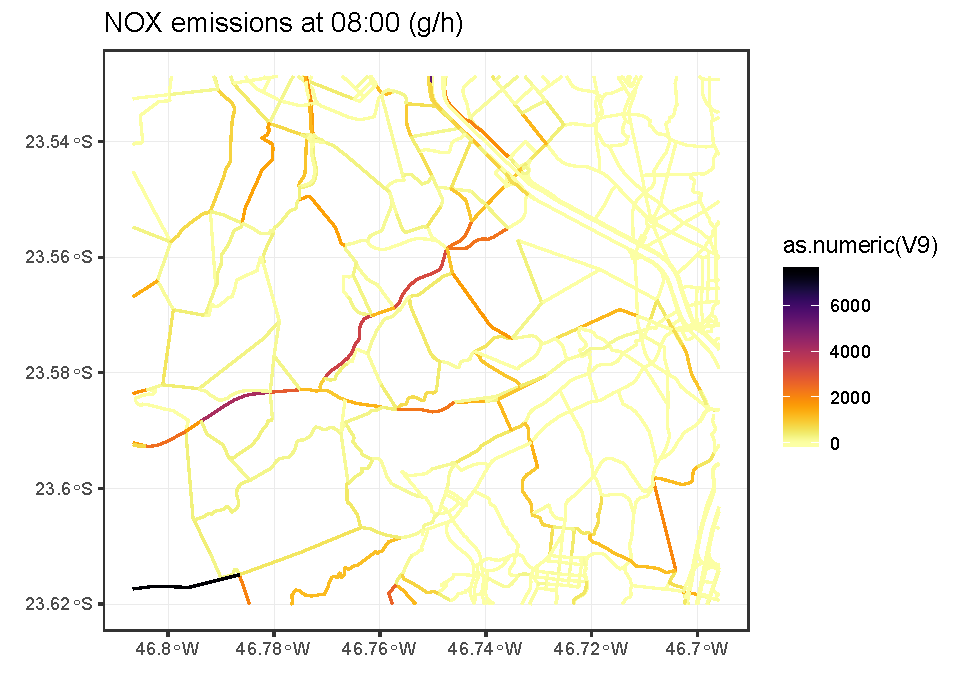
\includegraphics{veinbook_files/figure-latex/ltnox-1.pdf}
\caption{\label{fig:ltnox}NOx emisions of LT (g/h)}
\end{figure}

\section{Total emissions in
data-frames}\label{total-emissions-in-data-frames}

In order to obtain the total emissions in data-frame, the same function
\texttt{emis\_post} is used, but in this case, with the argument
\texttt{by} = ``veh''. We also need to add arguments of \texttt{veh} for
the type of vehicle, \texttt{size} the size or gross weight,
\texttt{fuel} and \texttt{pollutant}. The argument \texttt{net} is not
required in this case.

\begin{Shaded}
\begin{Highlighting}[]
\NormalTok{E_NOx_DF <-}\StringTok{ }\KeywordTok{emis_post}\NormalTok{(}\DataTypeTok{arra =}\NormalTok{ E_NOx, }\DataTypeTok{veh =} \StringTok{"LT"}\NormalTok{, }\DataTypeTok{size =} \StringTok{"Small"}\NormalTok{, }\DataTypeTok{fuel =} \StringTok{"B5"}\NormalTok{,}
                      \DataTypeTok{by =} \StringTok{"veh"}\NormalTok{, }\DataTypeTok{pollutant =} \StringTok{"NOx"}\NormalTok{)}
\KeywordTok{head}\NormalTok{(E_NOx_DF)}
\end{Highlighting}
\end{Shaded}

\begin{verbatim}
##     E_NOx              g veh  size fuel pollutant age hour
## 1 E_NOx_1 182.5943 [g/h]  LT Small   B5       NOx   1    1
## 2 E_NOx_2 163.2499 [g/h]  LT Small   B5       NOx   2    1
## 3 E_NOx_3 177.5608 [g/h]  LT Small   B5       NOx   3    1
## 4 E_NOx_4 208.5892 [g/h]  LT Small   B5       NOx   4    1
## 5 E_NOx_5 765.7001 [g/h]  LT Small   B5       NOx   5    1
## 6 E_NOx_6 885.6223 [g/h]  LT Small   B5       NOx   6    1
\end{verbatim}

The resulting object is a data-frame with the name of the input array,
then it has the g/h. Also, the name of the vehicle, the size, fuel,
pollutant, age and hour. This is interesting because we can now what are
the most pollutatn vehicle and at which hour this emissions ocurres.

\begin{Shaded}
\begin{Highlighting}[]
\NormalTok{E_NOx_DF[E_NOx_DF}\OperatorTok{$}\NormalTok{g }\OperatorTok{==}\StringTok{ }\KeywordTok{max}\NormalTok{(E_NOx_DF}\OperatorTok{$}\NormalTok{g), ]}
\end{Highlighting}
\end{Shaded}

\begin{verbatim}
##        E_NOx              g veh  size fuel pollutant age hour
## 517 E_NOx_17 29139.51 [g/h]  LT Small   B5       NOx  17   11
\end{verbatim}

The highest emissions by hour are of Light Trucks of 17 years of use at
hour 11 on local time. However, it is possible to get more interesting
insights of the data. The datra can be aggregated by age, hour or plot
all together as shown on Fig. \ref{fig:noxlt3}. The highest emissions
ocurre between 17 and 27 years of use. This figure also shows the effect
of emissions standards introduced in different years.

\begin{Shaded}
\begin{Highlighting}[]
\NormalTok{df <-}\StringTok{ }\KeywordTok{aggregate}\NormalTok{(E_NOx_DF}\OperatorTok{$}\NormalTok{g, }\DataTypeTok{by =} \KeywordTok{list}\NormalTok{(E_NOx_DF}\OperatorTok{$}\NormalTok{hour), sum)}
\KeywordTok{plot}\NormalTok{(df, }\DataTypeTok{type =} \StringTok{"b"}\NormalTok{, }\DataTypeTok{pch =} \DecValTok{16}\NormalTok{, }\DataTypeTok{xlab =} \StringTok{"hour"}\NormalTok{, }\DataTypeTok{ylab =} \StringTok{"NOx (g/h)"}\NormalTok{)}
\end{Highlighting}
\end{Shaded}

\begin{figure}
\centering
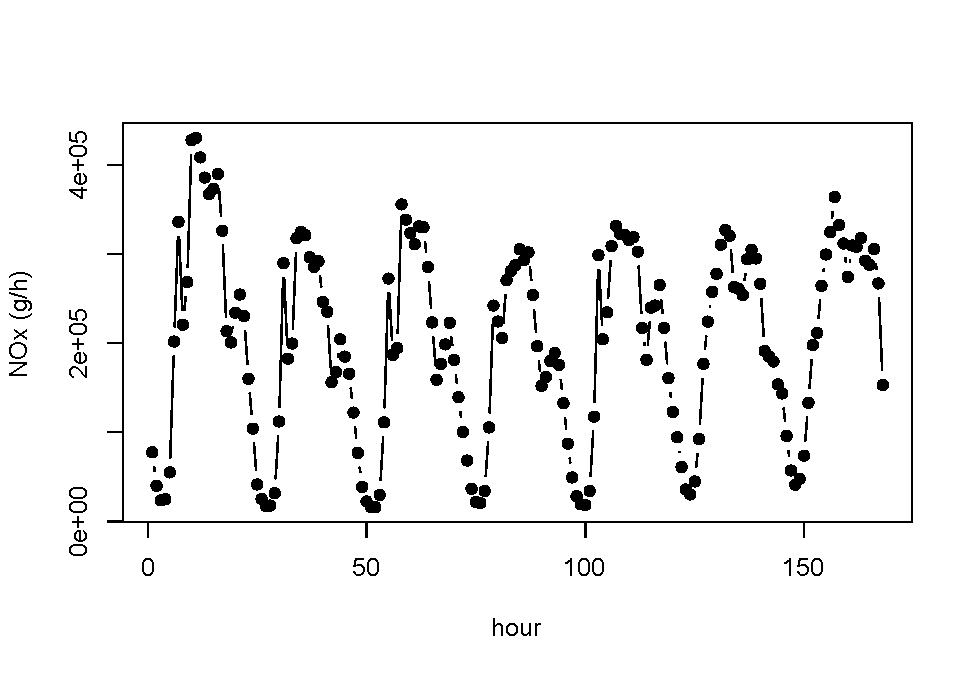
\includegraphics{veinbook_files/figure-latex/noxlt1-1.pdf}
\caption{\label{fig:noxlt1}NOx emissions of LT by hour}
\end{figure}

\begin{Shaded}
\begin{Highlighting}[]
\KeywordTok{library}\NormalTok{(ggplot2)}
\KeywordTok{library}\NormalTok{(veinreport) }\CommentTok{# theme_black}
\NormalTok{df <-}\StringTok{ }\KeywordTok{aggregate}\NormalTok{(E_NOx_DF}\OperatorTok{$}\NormalTok{g, }\DataTypeTok{by =} \KeywordTok{list}\NormalTok{(E_NOx_DF}\OperatorTok{$}\NormalTok{age), sum)}
\KeywordTok{names}\NormalTok{(df) <-}\StringTok{ }\KeywordTok{c}\NormalTok{(}\StringTok{"Age"}\NormalTok{, }\StringTok{"g"}\NormalTok{)}
\KeywordTok{ggplot}\NormalTok{(df, }\KeywordTok{aes}\NormalTok{(}\DataTypeTok{x =}\NormalTok{ Age, }\DataTypeTok{y =} \KeywordTok{as.numeric}\NormalTok{(g), }\DataTypeTok{fill =} \KeywordTok{as.numeric}\NormalTok{(g))) }\OperatorTok{+}
\StringTok{  }\KeywordTok{geom_bar}\NormalTok{(}\DataTypeTok{stat =} \StringTok{"identity"}\NormalTok{) }\OperatorTok{+}
\StringTok{  }\KeywordTok{scale_fill_gradientn}\NormalTok{(}\DataTypeTok{colours =} \KeywordTok{cpt}\NormalTok{()) }\OperatorTok{+}\StringTok{ }\KeywordTok{theme_black}\NormalTok{() }\OperatorTok{+}
\StringTok{  }\KeywordTok{labs}\NormalTok{(}\DataTypeTok{x =} \StringTok{"Age of use"}\NormalTok{, }\DataTypeTok{y =} \StringTok{"NOx (g/h)"}\NormalTok{)}
\end{Highlighting}
\end{Shaded}

\begin{figure}
\centering
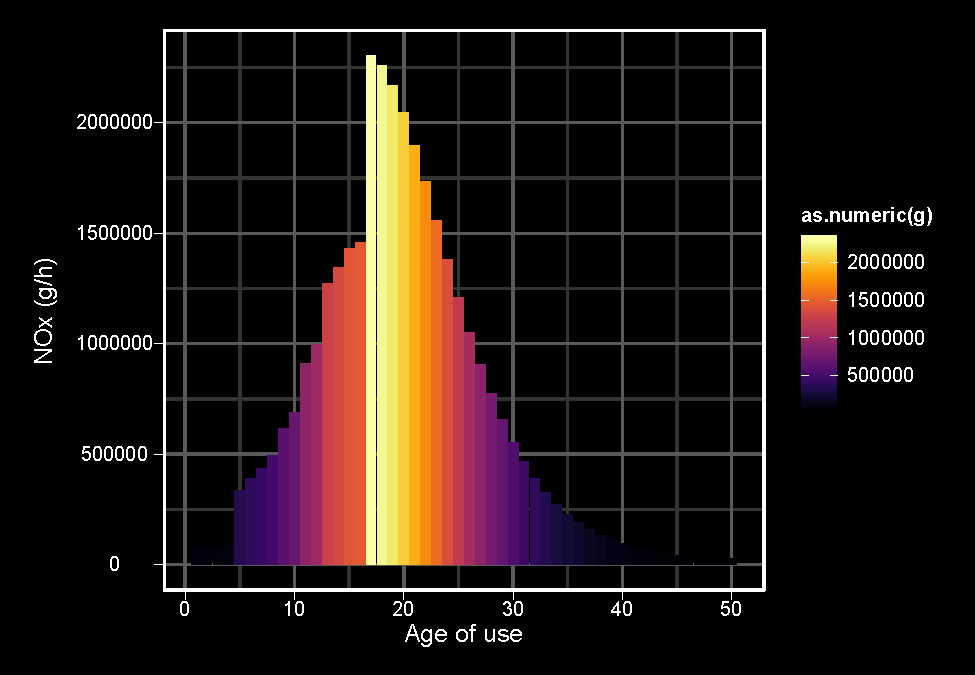
\includegraphics{veinbook_files/figure-latex/noxlt2-1.pdf}
\caption{\label{fig:noxlt2}NOx emissions of LT by age}
\end{figure}

\begin{Shaded}
\begin{Highlighting}[]
\KeywordTok{library}\NormalTok{(ggplot2)}
\KeywordTok{library}\NormalTok{(veinreport) }\CommentTok{# theme_black}
\KeywordTok{ggplot}\NormalTok{(E_NOx_DF, }\KeywordTok{aes}\NormalTok{(}\DataTypeTok{x =}\NormalTok{ age, }\DataTypeTok{y =} \KeywordTok{as.numeric}\NormalTok{(g), }\DataTypeTok{fill =}\NormalTok{ hour)) }\OperatorTok{+}
\StringTok{  }\KeywordTok{geom_bar}\NormalTok{(}\DataTypeTok{stat =} \StringTok{"identity"}\NormalTok{) }\OperatorTok{+}
\StringTok{  }\KeywordTok{scale_fill_gradientn}\NormalTok{(}\DataTypeTok{colours =} \KeywordTok{cpt}\NormalTok{()) }\OperatorTok{+}\StringTok{ }\KeywordTok{theme_black}\NormalTok{() }\OperatorTok{+}
\StringTok{  }\KeywordTok{labs}\NormalTok{(}\DataTypeTok{x =} \StringTok{"Age of use"}\NormalTok{, }\DataTypeTok{y =} \StringTok{"NOx (g/h)"}\NormalTok{)}
\end{Highlighting}
\end{Shaded}

\begin{figure}
\centering
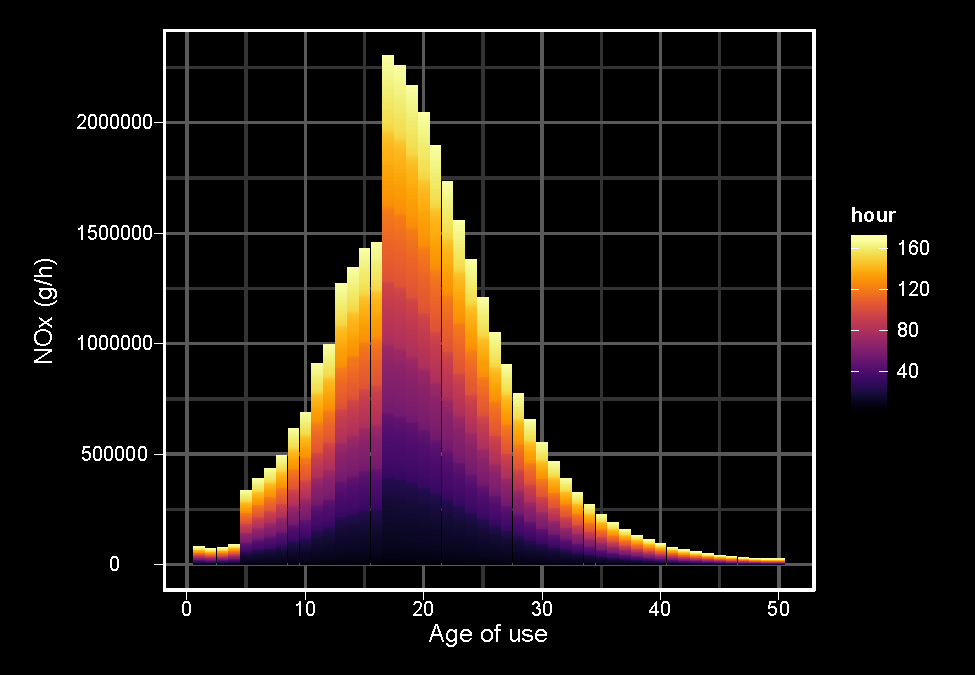
\includegraphics{veinbook_files/figure-latex/noxlt3-1.pdf}
\caption{\label{fig:noxlt3}NOx emissions of LT}
\end{figure}

\section{Merging emissions}\label{merging-emissions}

The function \texttt{inventory} was designed to store the emissions of
each type of vehicle in each directory. Hence, it was necessary to
create a function that read and merge the emissions that are in each
directory, returning a data-frame os a spatial feature data-frame. The
function is \texttt{emis\_merge}. As it can be seen on Fig.
\ref{fig:demispost}, \texttt{emis\_merge} comes after
\texttt{emis\_post} or \texttt{speciate}. The arguments of
\texttt{emis\_merge} are:

\begin{Shaded}
\begin{Highlighting}[]
\KeywordTok{args}\NormalTok{(vein}\OperatorTok{::}\NormalTok{emis_merge)}
\end{Highlighting}
\end{Shaded}

\begin{verbatim}
## function (pol = "CO", what = "STREETS.rds", streets = T, net, 
##     path = "emi", crs, under = "after", ignore = FALSE, as_list = FALSE) 
## NULL
\end{verbatim}

Where,

\begin{itemize}
\tightlist
\item
  \texttt{pol}: Character. Pollutant.
\item
  \texttt{what}: Character. Word to search the emissions names,
  ``STREETS'', ``DF'' or whatever name. It is important to include the
  extension .`rds'
\item
  \texttt{streets}: Logical. If true, emis\_merge will read the street
  emissions created with emis\_post by ``streets\_wide'', returning an
  object with class `sf'. If false, it will read the emissions
  data-frame and rbind them.
\item
  \texttt{net}: `Spatial feature' or `SpatialLinesDataFrame' with the
  streets. It is expected \#`that the number of rows is equal to the
  number of rows of street emissions. If \#' not, the function will
  stop.
\item
  \texttt{path}: Character. Path where emissions are located
\item
  \texttt{crs}: coordinate reference system in numeric format from
  \url{http://spatialreference.org/} to transform/project spatial data
  using sf::st\_transform
\end{itemize}

In order to see how this functions works, let's run the example in the
\texttt{inventory} function. First, lets create a project, or in other
words a directory named ``YourCity'', into the temporary directory. In
this part you can place your project wherever you want with the actual
name of your city. Then run \texttt{inventory} with the default
configuration.

\begin{Shaded}
\begin{Highlighting}[]
\NormalTok{name =}\StringTok{ }\KeywordTok{file.path}\NormalTok{(}\KeywordTok{tempdir}\NormalTok{(), }\StringTok{"YourCity"}\NormalTok{)}
\NormalTok{vein}\OperatorTok{::}\KeywordTok{inventory}\NormalTok{(}\DataTypeTok{name =}\NormalTok{ name, }\DataTypeTok{show.main =} \OtherTok{FALSE}\NormalTok{)}
\end{Highlighting}
\end{Shaded}

\begin{verbatim}
## files at /tmp/Rtmpxklera/YourCity
\end{verbatim}

\begin{verbatim}
## Directories:
##  [1] "/tmp/Rtmpxklera/YourCity"             
##  [2] "/tmp/Rtmpxklera/YourCity/ef"          
##  [3] "/tmp/Rtmpxklera/YourCity/emi"         
##  [4] "/tmp/Rtmpxklera/YourCity/emi/BUS_01"  
##  [5] "/tmp/Rtmpxklera/YourCity/emi/HGV_01"  
##  [6] "/tmp/Rtmpxklera/YourCity/emi/LCV_01"  
##  [7] "/tmp/Rtmpxklera/YourCity/emi/MC_01"   
##  [8] "/tmp/Rtmpxklera/YourCity/emi/PC_01"   
##  [9] "/tmp/Rtmpxklera/YourCity/est"         
## [10] "/tmp/Rtmpxklera/YourCity/images"      
## [11] "/tmp/Rtmpxklera/YourCity/network"     
## [12] "/tmp/Rtmpxklera/YourCity/post"        
## [13] "/tmp/Rtmpxklera/YourCity/post/df"     
## [14] "/tmp/Rtmpxklera/YourCity/post/grids"  
## [15] "/tmp/Rtmpxklera/YourCity/post/streets"
## [16] "/tmp/Rtmpxklera/YourCity/profiles"    
## [17] "/tmp/Rtmpxklera/YourCity/veh"
\end{verbatim}

In my case, the files are in directory /tmp/Rtmpxklera/YourCity. Now, if
you open the file file main.R, you will see:

\begin{center}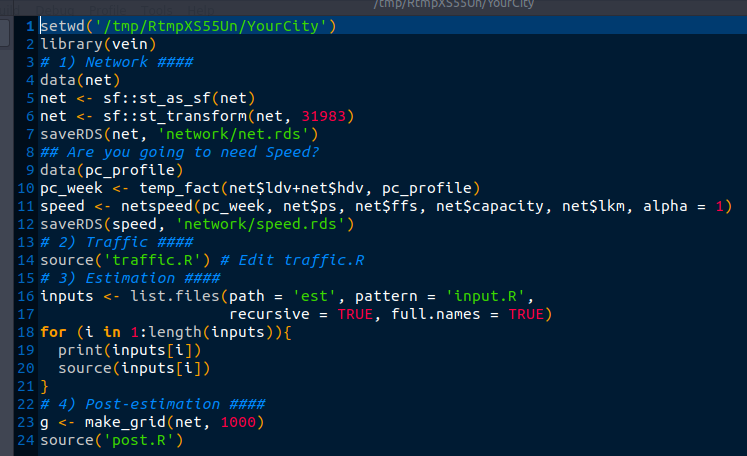
\includegraphics[width=0.7\linewidth]{figuras/main} \end{center}

This script starts with \texttt{setwd} function, Then the first section
is the network, where user reads and prepares the traffic information.
Then the second section runs a script whichruns the age functions for
the deault vehicular composition of the \texttt{inventory} function. The
third section estimates the emissions by running each input.R file
inside the directory \emph{est} The fourth section, creates a grid and
run the script post.R is shown below:

\begin{center}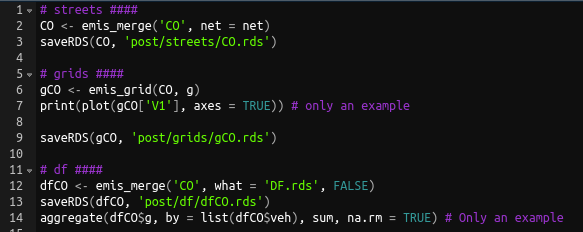
\includegraphics[width=0.7\linewidth]{figuras/post} \end{center}

The function \texttt{emis\_merge} shown in line 2 is designed to read
the all the files with names CO and the default argument \texttt{what}
is ``STREETS.rds'', for instance, PC\_GASOLINE\_CO\_STREETS.rds. Hence,
this function reads all the files under that condition. The other
argument is \texttt{streets} with defailt value of \texttt{TRUE},
meaning that the function now knows that the resulting object must be an
spatial network, and the \texttt{net} argument is already calling the
net object part of the VEIN data, the function will merge all the
objects summing the emissions of all vehicle street by street. The
resulting object is a spatial ``LINESTRING'' class of \texttt{sf}. This
function assumes that emissons files are data.frames and non tests have
been made to see if this function would read work \texttt{sf} objects.

On the other hand, the line 12 also runs all the emissions files whose
names includes the word CO, but also including the words ``DF.rds'',
which are the files from \texttt{emis\_post} with argument \texttt{by}
equals to ``veh''. In this case, it reads and merge the data-frames and
prints the sum emissions by pollutant.

If the user source he file main.R, it will calculate the emissions and
produce some plots.

\begin{Shaded}
\begin{Highlighting}[]
\KeywordTok{source}\NormalTok{(}\KeywordTok{paste0}\NormalTok{(name, }\StringTok{"/main.R"}\NormalTok{))}
\end{Highlighting}
\end{Shaded}

\section{Creating grids}\label{creating-grids}

Once we have processed our emissions array with \texttt{emis\_post}
and/or we have spatial emissions, we can then create grids and allocate
our emissions into the grids. Lets check the function
\texttt{make\_grid} first:

\begin{Shaded}
\begin{Highlighting}[]
\KeywordTok{args}\NormalTok{(vein}\OperatorTok{::}\NormalTok{make_grid)}
\end{Highlighting}
\end{Shaded}

\begin{verbatim}
## function (spobj, width, height = width, polygon, crs = 4326, 
##     ...) 
## NULL
\end{verbatim}

This function originally used an \texttt{sp} approach. However, now uses
an \texttt{sf} approach for creating the grid. Actually, the arguments
are pretty much the same with the \texttt{sf::st\_make\_grid} with the
exeption that is focused in returning polygons with coordinates at
centroids of each cell. Therefore, the arguments height and polygon are
deprecated. Lets create grid for our net.

\begin{Shaded}
\begin{Highlighting}[]
\KeywordTok{library}\NormalTok{(vein)}
\KeywordTok{library}\NormalTok{(sf)}
\KeywordTok{data}\NormalTok{(net)}
\NormalTok{net <-}\StringTok{ }\KeywordTok{st_transform}\NormalTok{(}\KeywordTok{st_as_sf}\NormalTok{(net), }\DecValTok{31983}\NormalTok{)}
\NormalTok{g <-}\StringTok{ }\KeywordTok{make_grid}\NormalTok{(}\DataTypeTok{spobj =}\NormalTok{ net, }\DataTypeTok{width =} \DecValTok{500}\NormalTok{)}
\end{Highlighting}
\end{Shaded}

\begin{verbatim}
## Number of lon points: 23
## Number of lat points: 21
\end{verbatim}

\begin{Shaded}
\begin{Highlighting}[]
\KeywordTok{class}\NormalTok{(g)}
\end{Highlighting}
\end{Shaded}

\begin{verbatim}
## [1] "sf"         "data.frame"
\end{verbatim}

\begin{Shaded}
\begin{Highlighting}[]
\KeywordTok{plot}\NormalTok{(g}\OperatorTok{$}\NormalTok{geometry, }\DataTypeTok{axes =} \OtherTok{TRUE}\NormalTok{)}
\KeywordTok{plot}\NormalTok{(net}\OperatorTok{$}\NormalTok{geometry, }\DataTypeTok{add =} \OtherTok{TRUE}\NormalTok{)}
\end{Highlighting}
\end{Shaded}

\begin{figure}
\centering
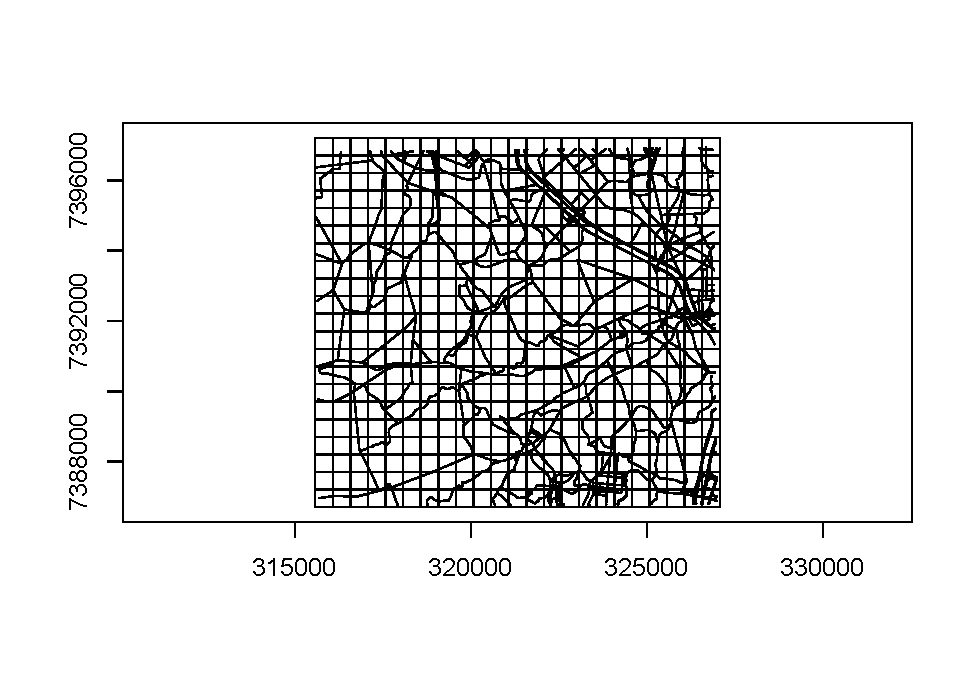
\includegraphics{veinbook_files/figure-latex/grid1-1.pdf}
\caption{\label{fig:grid1}Grid with spacing of 500 mts}
\end{figure}

The class of \texttt{net} is \texttt{SpatialLinesDataFrame}, which is
converted to \texttt{sf}. Then, as the coordinte reference system of net
is WGS84 with epsg 4326, we are transforming to UTM to create a grid
with grid spacing of 500 mts. The class of the grid object, \texttt{g}
is ``sf data.frame''.

\section{\texorpdfstring{Gridding bottom-up emissions with
\texttt{emis\_grid}}{Gridding bottom-up emissions with emis\_grid}}\label{gridding-bottom-up-emissions-with-emis_grid}

The function\texttt{emis\_grid} allocates emissions proportionally to
each grid cell. The process is performed by intersection between
geometries and the grid. It means that requires ``sr'' according with
your location for the projection. It is assumed that spobj is a
spatial*DataFrame or an ``sf'' with the pollutants in data. This
function return an object class ``sf''.

Before \texttt{sf} era, i tried to use\texttt{raster::intersect} which
imports \texttt{rgeos} and took \textbf{ages}. Then I started to use
\citet{QGIS} (\url{https://www.qgis.org}), and later the R package
\citet{RQGIS} which takes 10 minutes for allocating emissions of the
mega-city of São Paulo and a grid spacing of 1 km. \emph{10 min is not
bad}. However, when \texttt{sf} appeared and also, included the Spatial
Indexes
(\url{https://www.r-spatial.org/r/2017/06/22/spatial-index.html}), it
changed the game. A new era started. It took \textbf{5.5 seconds}. I
could not believe it. But there also some i could accelerate this
process importing some \texttt{data.table} aggregation functions. Now
\texttt{emis\_grid} can aggegate big spatial extensions. I havent tried
yet at continental scale, but I will try. Anyways, let's go see the
arguments:

\begin{Shaded}
\begin{Highlighting}[]
\KeywordTok{args}\NormalTok{(vein}\OperatorTok{::}\NormalTok{emis_grid)}
\end{Highlighting}
\end{Shaded}

\begin{verbatim}
## function (spobj, g, sr, type = "lines") 
## NULL
\end{verbatim}

Where,

\begin{itemize}
\tightlist
\item
  \texttt{spobj} : A spatial dataframe of class ``sp'' or ``sf''. When
  class is ``sp'' it is transformed to ``sf''.
\item
  \texttt{g}: A grid with class ``SpatialPolygonsDataFrame'' or ``sf''.
\item
  \texttt{sr}: Spatial reference e.g: 31983. It is required if spobj and
  g are not projected. Please, see \url{http://spatialreference.org/}.
\item
  \texttt{type}: type of geometry: ``lines'' or ``points''.
\end{itemize}

\begin{Shaded}
\begin{Highlighting}[]
\KeywordTok{data}\NormalTok{(net)}
\NormalTok{net}\OperatorTok{@}\NormalTok{data <-}\StringTok{ }\KeywordTok{data.frame}\NormalTok{(}\DataTypeTok{hdv =}\NormalTok{ net[[}\StringTok{"hdv"}\NormalTok{]])}
\NormalTok{g <-}\StringTok{ }\KeywordTok{make_grid}\NormalTok{(}\DataTypeTok{spobj =}\NormalTok{ net, }\DataTypeTok{width =} \DecValTok{1}\OperatorTok{/}\FloatTok{102.47}\OperatorTok{/}\DecValTok{2}\NormalTok{)}
\end{Highlighting}
\end{Shaded}

\begin{verbatim}
## Number of lon points: 23
## Number of lat points: 19
\end{verbatim}

\begin{Shaded}
\begin{Highlighting}[]
\NormalTok{netg <-}\StringTok{ }\KeywordTok{emis_grid}\NormalTok{(net, g)}
\end{Highlighting}
\end{Shaded}

\begin{verbatim}
## Sum of street emissions 148118
\end{verbatim}

\begin{verbatim}
## although coordinates are longitude/latitude, st_intersection assumes that they are planar
\end{verbatim}

\begin{verbatim}
## Sum of gridded emissions 148118
\end{verbatim}

\begin{Shaded}
\begin{Highlighting}[]
\KeywordTok{head}\NormalTok{(netg)}
\end{Highlighting}
\end{Shaded}

\begin{verbatim}
## Simple feature collection with 6 features and 2 fields
## geometry type:  POLYGON
## dimension:      XY
## bbox:           xmin: -46.8066 ymin: -23.62 xmax: -46.77732 ymax: -23.61512
## epsg (SRID):    4326
## proj4string:    +proj=longlat +datum=WGS84 +no_defs
##   id      hdv                       geometry
## 1  1 201.8275 POLYGON ((-46.8066 -23.62, ...
## 2  2 200.6097 POLYGON ((-46.80172 -23.62,...
## 3  3 205.6319 POLYGON ((-46.79684 -23.62,...
## 4  4 224.1988 POLYGON ((-46.79196 -23.62,...
## 5  5 770.9490 POLYGON ((-46.78708 -23.62,...
## 6  6   0.0000 POLYGON ((-46.7822 -23.62, ...
\end{verbatim}

\begin{Shaded}
\begin{Highlighting}[]
\KeywordTok{plot}\NormalTok{(netg[}\StringTok{"hdv"}\NormalTok{], }\DataTypeTok{axes =} \OtherTok{TRUE}\NormalTok{)}
\end{Highlighting}
\end{Shaded}

\begin{figure}
\centering
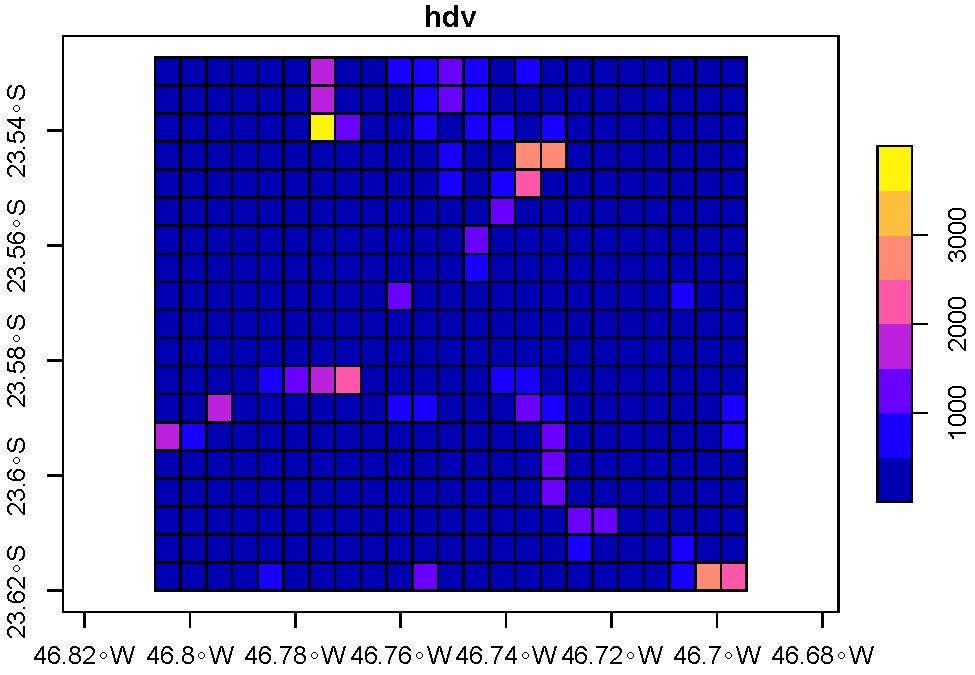
\includegraphics{veinbook_files/figure-latex/netgldv-1.pdf}
\caption{\label{fig:netgldv}Spatial grid of HDV traffic 500 mts}
\end{figure}

The example in this case, showed the allocation of traffic. The
resulting object is a \texttt{sf} with the sum of the attributes inside
each grid cell. This means that, when the input are street emissions at
different hours, it will return gridded emissions at each hour:

\begin{Shaded}
\begin{Highlighting}[]
\NormalTok{E_NOx_STREETS <-}\StringTok{ }\KeywordTok{emis_post}\NormalTok{(E_NOx, }\DataTypeTok{by =} \StringTok{"streets_wide"}\NormalTok{, }\DataTypeTok{net =}\NormalTok{ net)}
\NormalTok{NOxg <-}\StringTok{ }\KeywordTok{emis_grid}\NormalTok{(E_NOx_STREETS, g)}
\end{Highlighting}
\end{Shaded}

\begin{verbatim}
## Sum of street emissions 34029872.64
\end{verbatim}

\begin{verbatim}
## although coordinates are longitude/latitude, st_intersection assumes that they are planar
\end{verbatim}

\begin{verbatim}
## Sum of gridded emissions 34029872.64
\end{verbatim}

\begin{Shaded}
\begin{Highlighting}[]
\KeywordTok{plot}\NormalTok{(NOxg[}\StringTok{"V1"}\NormalTok{], }\DataTypeTok{axes =} \OtherTok{TRUE}\NormalTok{)}
\end{Highlighting}
\end{Shaded}

\begin{figure}
\centering
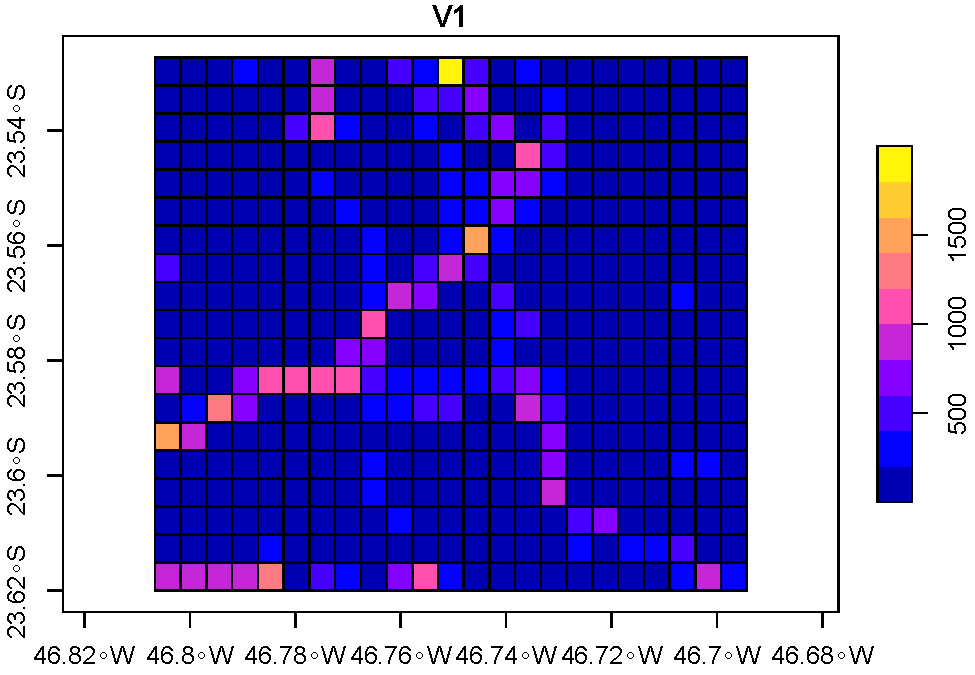
\includegraphics{veinbook_files/figure-latex/Noxg-1.pdf}
\caption{\label{fig:Noxg}NOx emissions for 00:00 {[}g/h{]}}
\end{figure}

\section{\texorpdfstring{Gridding top-down emissions with
\texttt{emis\_dist}}{Gridding top-down emissions with emis\_dist}}\label{gridding-top-down-emissions-with-emis_dist}

When a top-down approach emissions inventory is made, the spatial
distribution of emissions must be made considering some proxy. In the
case of vehicular emissions, it can be done with data of Open Street
Maps,distributing the emissions into the streets. This can be done with
the function with the function \texttt{emis\_dist}. In generaly, this
function distribute the emissions into spatial feature on any type, not
only lines.

\begin{Shaded}
\begin{Highlighting}[]
\KeywordTok{args}\NormalTok{(vein}\OperatorTok{::}\NormalTok{emis_dist)}
\end{Highlighting}
\end{Shaded}

\begin{verbatim}
## function (gy, spobj, pro, osm, verbose = TRUE) 
## NULL
\end{verbatim}

Where,

\begin{itemize}
\tightlist
\item
  \texttt{gy}: Numeric; a unique total (top-down) emissions (grams)
\item
  \texttt{spobj}: A spatial dataframe of class ``sp'' or ``sf''. When
  class is ``sp'' it is transformed to ``sf''.
\item
  \texttt{pro}: Matrix or data-frame profiles, for instance,
  pc\_profile.
\item
  \texttt{osm}: Numeric; vector of length 5, for instance, c(5, 3, 2, 1,
  1). The first element covers `motorway' and `motorway\_link. The
  second element covers 'trunk' and `trunk\_link'. The third element
  covers `primary' and `primary\_link'. The fourth element covers
  `secondary' and `secondary\_link'. The fifth element covers `tertiary'
  and `tertiary\_link'.
\item
  \texttt{verbose}: Logical; to show more info.
\end{itemize}

In order test this function, it will be used the function
\texttt{osmdata}. The process presented in the following code, consists
in downloading the openstreetmap data delimited by the coordenaes og the
grid \texttt{g}. Then filter only the lines

\begin{Shaded}
\begin{Highlighting}[]
\KeywordTok{library}\NormalTok{(osmdata)}
\KeywordTok{library}\NormalTok{(sf, }\DataTypeTok{quietly =}\NormalTok{ T)}
\NormalTok{osm <-}\StringTok{ }\KeywordTok{osmdata_sf}\NormalTok{(}
  \KeywordTok{add_osm_feature}\NormalTok{(}
    \KeywordTok{opq}\NormalTok{(}\DataTypeTok{bbox =} \KeywordTok{st_bbox}\NormalTok{(g)),                             }
    \DataTypeTok{key =} \StringTok{'highway'}\NormalTok{))}\OperatorTok{$}\NormalTok{osm_lines[, }\KeywordTok{c}\NormalTok{(}\StringTok{"highway"}\NormalTok{)]}
\NormalTok{st <-}\StringTok{ }\KeywordTok{c}\NormalTok{(}\StringTok{"motorway"}\NormalTok{, }\StringTok{"motorway_link"}\NormalTok{, }\StringTok{"}
\StringTok{        trunk"}\NormalTok{, }\StringTok{"trunk_link"}\NormalTok{, }
        \StringTok{"primary"}\NormalTok{, }\StringTok{"primary_link"}\NormalTok{, }
        \StringTok{"secondary"}\NormalTok{, }\StringTok{"secondary_link"}\NormalTok{, }
        \StringTok{"tertiary"}\NormalTok{, }\StringTok{"tertiary_link"}\NormalTok{)}
\NormalTok{osm <-}\StringTok{ }\NormalTok{osm[osm}\OperatorTok{$}\NormalTok{highway }\OperatorTok\StringTok{ }\NormalTok{st, ]}
\KeywordTok{plot}\NormalTok{(osm, }\DataTypeTok{axes =}\NormalTok{ T)}
\end{Highlighting}
\end{Shaded}

\begin{figure}
\centering
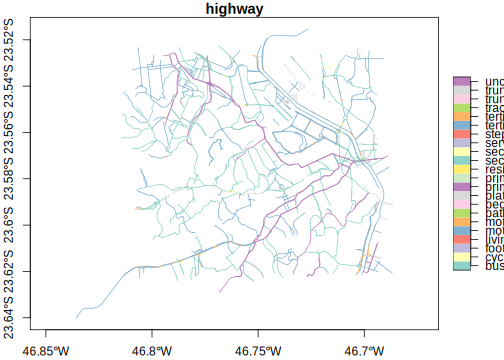
\includegraphics{veinbook_files/figure-latex/osmsp-1.pdf}
\caption{\label{fig:osmsp}Open street map lines}
\end{figure}

The we will distribute the total emissions of E\_NOx
3.4029873\times 10\^{}\{7\} into this new lines. There is the argument
osm, which gives percentage weights to the type of streets in the
following order: ``motorway'', ``trunk'', ``primary'', ``secondary'' and
``tertiary'' . For instance \textbf{osm = 5:1} means 33\% of emissions
into ``motorway'' because it is 5 / (1 + 2 + 3 + 4 + 5).

\begin{Shaded}
\begin{Highlighting}[]
\NormalTok{estreet <-}\StringTok{ }\KeywordTok{emis_dist}\NormalTok{(}\DataTypeTok{gy =} \KeywordTok{sum}\NormalTok{(E_NOx), }\DataTypeTok{spobj =}\NormalTok{ osm)}
\end{Highlighting}
\end{Shaded}

\begin{verbatim}
## Columns: geometry emission
\end{verbatim}

\begin{Shaded}
\begin{Highlighting}[]
\NormalTok{estreet}\OperatorTok{$}\NormalTok{emission_osm <-}\StringTok{ }\KeywordTok{emis_dist}\NormalTok{(}\DataTypeTok{gy =} \KeywordTok{sum}\NormalTok{(E_NOx), }\DataTypeTok{spobj =}\NormalTok{ osm, }
                                   \DataTypeTok{osm =} \DecValTok{5}\OperatorTok{:}\DecValTok{1}\NormalTok{)}\OperatorTok{$}\NormalTok{emission}
\end{Highlighting}
\end{Shaded}

\begin{verbatim}
## Selecting: motorway motorway_link trunk trunk_link primary primary_link secondary secondary_link tertiary tertiary_link 
## Columns: emission highway geometry
\end{verbatim}

\begin{Shaded}
\begin{Highlighting}[]
\KeywordTok{plot}\NormalTok{(estreet[}\KeywordTok{c}\NormalTok{(}\StringTok{"emission"}\NormalTok{)], }
     \DataTypeTok{main =} \KeywordTok{paste0}\NormalTok{(}\StringTok{"Emissions with Default distribution: "}\NormalTok{,}
                   \KeywordTok{round}\NormalTok{(}\KeywordTok{sum}\NormalTok{(estreet}\OperatorTok{$}\NormalTok{emission)), }\StringTok{" [g]"}\NormalTok{), }
     \DataTypeTok{axes =}\NormalTok{ T,}\DataTypeTok{pal =} \KeywordTok{cpt}\NormalTok{(}\DataTypeTok{colorRampPalette =}\NormalTok{ T))}
\end{Highlighting}
\end{Shaded}

\begin{figure}
\centering
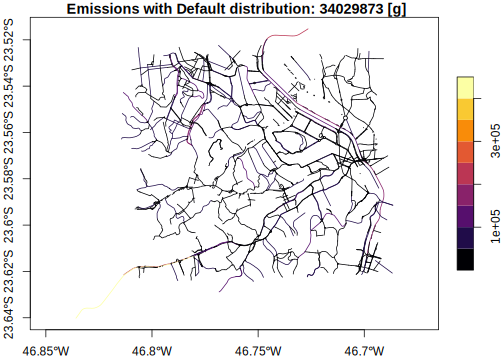
\includegraphics{veinbook_files/figure-latex/osmemi-1.pdf}
\caption{\label{fig:osmemi}Emissions distributed into OSM lines}
\end{figure}

\begin{Shaded}
\begin{Highlighting}[]
\KeywordTok{plot}\NormalTok{(estreet[}\KeywordTok{c}\NormalTok{(}\StringTok{"emission_osm"}\NormalTok{)],}
          \DataTypeTok{main =} \KeywordTok{paste0}\NormalTok{(}\StringTok{"Emission with OSM distribution: "}\NormalTok{,}
                        \KeywordTok{round}\NormalTok{(}\KeywordTok{sum}\NormalTok{(estreet}\OperatorTok{$}\NormalTok{emission_osm)), }\StringTok{" [g]"}\NormalTok{),  }
     \DataTypeTok{axes =}\NormalTok{ T,}\DataTypeTok{pal =} \KeywordTok{cpt}\NormalTok{(}\DataTypeTok{colorRampPalette =}\NormalTok{ T))}
\end{Highlighting}
\end{Shaded}

\begin{figure}
\centering
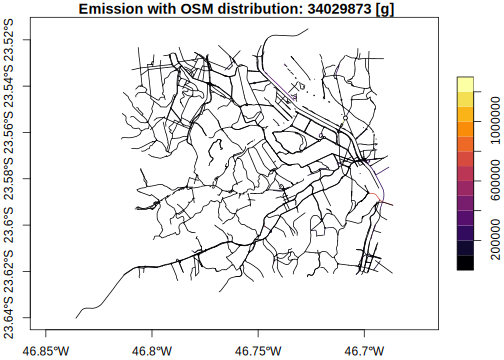
\includegraphics{veinbook_files/figure-latex/osmemi-2.pdf}
\caption{\label{fig:osmemi}Emissions distributed into OSM lines}
\end{figure}

\section{\texorpdfstring{Gridding top-down emissions with
\texttt{grid\_emis}}{Gridding top-down emissions with grid\_emis}}\label{gridding-top-down-emissions-with-grid_emis}

Another option to distribute top-down emissions consits in the use of
the function \texttt{grid\_emis}, which does a similar job than
\texttt{emis\_dist} but cell by cell. This means that the total
emissions are distributed inside each grid cell and not one distribution
for the whole domain. This functions runs a lapply of
\texttt{emis\_dist}, hence it takes a litle bit of more time.

\begin{Shaded}
\begin{Highlighting}[]
\KeywordTok{args}\NormalTok{(vein}\OperatorTok{::}\NormalTok{grid_emis)}
\end{Highlighting}
\end{Shaded}

\begin{verbatim}
## function (spobj, g, sr, pro, osm, verbose = TRUE) 
## NULL
\end{verbatim}

Where,

\begin{itemize}
\tightlist
\item
  \texttt{spobj}: A spatial dataframe of class ``sp'' or ``sf''. When
  class is ``sp'' it is transformed to ``sf''.
\item
  \texttt{g}: A grid with class ``SpatialPolygonsDataFrame'' or ``sf''.
  This grid includes the total emissions with the column ``emission''.
  If profile is going to be used, the column `emission' must include the
  sum of the emissions for each profile. For instance, if profile covers
  the hourly emissions, the column `emission' bust be the sum of the
  hourly emissions.
\item
  \texttt{sr}: Spatial reference e.g: 31983. It is required if spobj and
  g are not projected. Please, see \url{http://spatialreference.org/}.
\item
  \texttt{pro}: Numeric, Matrix or data-frame profiles, for instance,
  pc\_profile.
\item
  \texttt{osm}: Numeric; vector of length 5, for instance, c(5, 3, 2, 1,
  1). The first element covers `motorway' and `motorway\_link. The
  second element covers 'trunk' and `trunk\_link'. The third element
  covers `primary' and `primary\_link'. The fourth element covers
  `secondary' and `secondary\_link'. The fifth element covers `tertiary'
  and `tertiary\_link'.
\item
  \texttt{verbose}: Logical; to show more info.
\end{itemize}

It is required that the grid

\begin{Shaded}
\begin{Highlighting}[]
\NormalTok{NOxg <-}\StringTok{ }\NormalTok{NOxg[, }\StringTok{"V1"}\NormalTok{]}
\KeywordTok{names}\NormalTok{(NOxg)[}\DecValTok{1}\NormalTok{] <-}\StringTok{ "emission"}
\NormalTok{xnet <-}\StringTok{ }\KeywordTok{grid_emis}\NormalTok{(osm, NOxg)}
\end{Highlighting}
\end{Shaded}

\begin{verbatim}
## although coordinates are longitude/latitude, st_intersection assumes that they are planar
\end{verbatim}

\begin{verbatim}
## Sum of gridded emissions 77253.6
## Sum of street emissions 77253.6
## Columns: emission geometry
\end{verbatim}

\begin{Shaded}
\begin{Highlighting}[]
\KeywordTok{plot}\NormalTok{(xnet, }\DataTypeTok{axes =}\NormalTok{ T,}\DataTypeTok{pal =} \KeywordTok{cpt}\NormalTok{(}\DataTypeTok{colorRampPalette =}\NormalTok{ T))}
\end{Highlighting}
\end{Shaded}

\begin{figure}
\centering
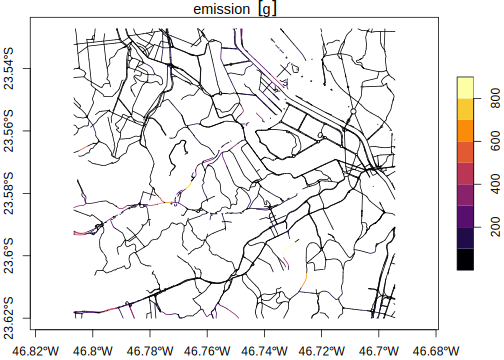
\includegraphics{veinbook_files/figure-latex/osmspgrid-1.pdf}
\caption{\label{fig:osmspgrid}Use of grid\_emis}
\end{figure}

\chapter{Speciation}\label{he}

The speciation for emissions is a very important part that deserves a
only chapter on this book. VEIN initially covered speed functions
emission factors of CO, HC, NOx, PM and Fuel Consumption (FC). But
currently, the the pollutants covered are:

\begin{itemize}
\tightlist
\item
  \textbf{Criteria}: ``CO'', ``NOx'', ``HC'', ``PM'', ``CH4'', ``NMHC'',
  ``CO2'', ``SO2'', ``Pb'', ``FC'' (Fuel Consumption).
\item
  \textbf{Polycyclic Aromatic Hydrocarbons (PAH) and Persisten Organic
  Pollutants (POP)}: ``indeno(1,2,3-cd)pyrene'',
  ``benzo(k)fluoranthene'', ``benzo(b)fluoranthene'',
  ``benzo(ghi)perylene'', ``fluoranthene'', ``benzo(a)pyrene'',
  ``pyrene'', ``perylene'', ``anthanthrene'', ``benzo(b)fluorene'',
  ``benzo(e)pyrene'', ``triphenylene'', ``benzo(j)fluoranthene'',
  ``dibenzo(a,j)anthacene'', ``dibenzo(a,l)pyrene'',
  ``3,6-dimethyl-phenanthrene'', ``benzo(a)anthracene'',
  ``acenaphthylene'', ``acenapthene'', ``fluorene'', ``chrysene'',
  ``phenanthrene'', ``napthalene'', ``anthracene'', ``coronene'',
  ``dibenzo(ah)anthracene''
\item
  \textbf{Dioxins and Furans}: ``PCDD'', ``PCDF'', ``PCB''.
\item
  \textbf{Metals}: ``As'', ``Cd'', ``Cr'', ``Cu'', ``Hg'', ``Ni'',
  ``Pb'', ``Se'', ``Zn''.
\item
  \textbf{NMHC}:
\item
  \emph{ALKANES}: ``ethane'', ``propane'', ``butane'', ``isobutane'',
  ``pentane'', ``isopentane'', ``hexane'', ``heptane'', ``octane'',
  ``TWO\_methylhexane'', ``nonane'', ``TWO\_methylheptane'',
  ``THREE\_methylhexane'', ``decane'', ``THREE\_methylheptane'',
  ``alcanes\_C10\_C12'', ``alkanes\_C13''.
\item
  \emph{CYCLOALKANES}: ``cycloalcanes''.
\item
  \emph{ALKENES}: ``ethylene'', ``propylene'', ``propadiene'',
  ``ONE\_butene'', ``isobutene'', ``TWO\_butene'',
  ``ONE\_3\_butadiene'', ``ONE\_pentene'', ``TWO\_pentene'',
  ``ONE\_hexene'', ``dimethylhexene''.
\item
  \emph{ALKYNES}:``ONE\_butine'', ``propine'', ``acetylene''.
\item
  \emph{ALDEHYDES}: ``formaldehyde'', ``acetaldehyde'', ``acrolein'',
  ``benzaldehyde'', ``crotonaldehyde'', ``methacrolein'',
  ``butyraldehyde'', ``isobutanaldehyde'', ``propionaldehyde'',
  ``hexanal'', ``i\_valeraldehyde'', ``valeraldehyde'',
  ``o\_tolualdehyde'', ``m\_tolualdehyde'', ``p\_tolualdehyde''.
\item
  KETONES: ``acetone'', ``methylethlketone''.
\item
  \emph{AROMATICS}: ``toluene'', ``ethylbenzene'', ``m\_p\_xylene'',
  ``o\_xylene'', ``ONE\_2\_3\_trimethylbenzene'',
  ``ONE\_2\_4\_trimethylbenzene'', ``ONE\_3\_5\_trimethylbenzene'',
  ``styrene'', ``benzene'', ``C9'', ``C10'', ``C13''.
\end{itemize}

Also, some Brazilian emission factors and speciations for WRF-Chem,
mechanisms: ``e\_eth'', ``e\_hc3'', ``e\_hc5'', ``e\_hc8'', ``e\_ol2'',
``e\_olt'', ``e\_oli'', ``e\_iso'', ``e\_tol'', ``e\_xyl'',
``e\_c2h5oh'', ``e\_ald'', ``e\_hcho'', ``e\_ch3oh'', ``e\_ket'',
``E\_SO4i'', ``E\_SO4j'', ``E\_NO3i'', ``E\_NO3j'', ``E\_MP2.5i'',
``E\_MP2.5j'', ``E\_ORGi'', ``E\_ORGj'', ``E\_ECi'', ``E\_ECj'',
``H2O''.

By the end of this book, more emission factors will be added.

Because VEIN has the capabilities to produce species from this
pollutants including volatile organic compunds (VOC) and particulate
matter compounds.

The speciation of emissions in VEIN can be done with three ways, by
selecting the pollutants in ef\_speed* functions, other way explicit and
the other implicit. The explicit way is by usint the function
\texttt{speciate} for the specific available speciation. The implicit
way is by adding a percentage value in the argument \texttt{k} in any of
the functions of emission factors. The implicit way requires that the
user must know the percentage of the species of pollutant.

\section{Speed functions of VOC
species}\label{speed-functions-of-voc-species}

As mentioned before, the speed function emission factors, currently
covers several pollutants. We firstly focus on som PAH and POP. They way
to select them is just:

\begin{Shaded}
\begin{Highlighting}[]
\KeywordTok{library}\NormalTok{(vein)}
\NormalTok{pol <-}\StringTok{ }\KeywordTok{c}\NormalTok{(}\StringTok{"indeno(1,2,3-cd)pyrene"}\NormalTok{, }\StringTok{"benzo(k)fluoranthene"}\NormalTok{,}
         \StringTok{"benzo(b)fluoranthene"}\NormalTok{, }\StringTok{"benzo(ghi)perylene"}\NormalTok{, }\StringTok{"fluoranthene"}\NormalTok{,}
         \StringTok{"benzo(a)pyrene"}\NormalTok{)}
\NormalTok{df <-}\StringTok{ }\KeywordTok{lapply}\NormalTok{(}\DecValTok{1}\OperatorTok{:}\KeywordTok{length}\NormalTok{(pol), }\ControlFlowTok{function}\NormalTok{(i)\{}
  \KeywordTok{EmissionFactors}\NormalTok{(}\KeywordTok{ef_ldv_speed}\NormalTok{(}\StringTok{"PC"}\NormalTok{, }\StringTok{"4S"}\NormalTok{, }\StringTok{"<=1400"}\NormalTok{, }\StringTok{"G"}\NormalTok{, }\StringTok{"PRE"}\NormalTok{,}
\NormalTok{                               pol[i], }\DataTypeTok{x =} \DecValTok{10}\NormalTok{)(}\DecValTok{10}\NormalTok{))}
\NormalTok{\})}
\KeywordTok{names}\NormalTok{(df) <-}\StringTok{ }\NormalTok{pol}
\NormalTok{df}
\end{Highlighting}
\end{Shaded}

\begin{verbatim}
## $`indeno(1,2,3-cd)pyrene`
## 1.03e-06 [g/km]
## 
## $`benzo(k)fluoranthene`
## 3e-07 [g/km]
## 
## $`benzo(b)fluoranthene`
## 8.8e-07 [g/km]
## 
## $`benzo(ghi)perylene`
## 2.9e-06 [g/km]
## 
## $fluoranthene
## 1.822e-05 [g/km]
## 
## $`benzo(a)pyrene`
## 4.8e-07 [g/km]
\end{verbatim}

These pollutants comes from \citet{NtziachristosSamaras2016} and in this
case, are not dependent on speed. I used lapply to iterate in each
pollutant at 10 km/h. Now I will show the same for dioxins and furans.

\begin{Shaded}
\begin{Highlighting}[]
\KeywordTok{library}\NormalTok{(vein)}
\NormalTok{pol <-}\StringTok{ }\KeywordTok{c}\NormalTok{(}\StringTok{"PCDD"}\NormalTok{, }\StringTok{"PCDF"}\NormalTok{, }\StringTok{"PCB"}\NormalTok{)}
\NormalTok{df <-}\StringTok{ }\KeywordTok{lapply}\NormalTok{(}\DecValTok{1}\OperatorTok{:}\KeywordTok{length}\NormalTok{(pol), }\ControlFlowTok{function}\NormalTok{(i)\{}
  \KeywordTok{EmissionFactors}\NormalTok{(}\KeywordTok{ef_ldv_speed}\NormalTok{(}\StringTok{"PC"}\NormalTok{, }\StringTok{"4S"}\NormalTok{, }\StringTok{"<=1400"}\NormalTok{, }\StringTok{"G"}\NormalTok{, }\StringTok{"PRE"}\NormalTok{,}
\NormalTok{                               pol[i], }\DataTypeTok{x =} \DecValTok{10}\NormalTok{)(}\DecValTok{10}\NormalTok{))}
\NormalTok{\})}
\KeywordTok{names}\NormalTok{(df) <-}\StringTok{ }\NormalTok{pol}
\NormalTok{df}
\end{Highlighting}
\end{Shaded}

\begin{verbatim}
## $PCDD
## 1.03e-11 [g/km]
## 
## $PCDF
## 2.12e-11 [g/km]
## 
## $PCB
## 6.4e-12 [g/km]
\end{verbatim}

In the case of nmhc, the estimation is:

\begin{Shaded}
\begin{Highlighting}[]
\KeywordTok{library}\NormalTok{(vein)}
\NormalTok{pol <-}\StringTok{ }\KeywordTok{c}\NormalTok{(}\StringTok{"ethane"}\NormalTok{, }\StringTok{"propane"}\NormalTok{, }\StringTok{"butane"}\NormalTok{, }\StringTok{"isobutane"}\NormalTok{, }\StringTok{"pentane"}\NormalTok{)}
\NormalTok{df <-}\StringTok{ }\KeywordTok{lapply}\NormalTok{(}\DecValTok{1}\OperatorTok{:}\KeywordTok{length}\NormalTok{(pol), }\ControlFlowTok{function}\NormalTok{(i)\{}
  \KeywordTok{EmissionFactors}\NormalTok{(}\KeywordTok{ef_ldv_speed}\NormalTok{(}\StringTok{"PC"}\NormalTok{, }\StringTok{"4S"}\NormalTok{, }\StringTok{"<=1400"}\NormalTok{, }\StringTok{"G"}\NormalTok{, }\StringTok{"PRE"}\NormalTok{,}
\NormalTok{                               pol[i], }\DataTypeTok{x =} \DecValTok{10}\NormalTok{)(}\KeywordTok{c}\NormalTok{(}\DecValTok{10}\NormalTok{,}\DecValTok{20}\NormalTok{,}\DecValTok{30}\NormalTok{)))}
\NormalTok{\})}
\KeywordTok{names}\NormalTok{(df) <-}\StringTok{ }\NormalTok{pol}
\NormalTok{df}
\end{Highlighting}
\end{Shaded}

\begin{verbatim}
## $ethane
## Units: [g/km]
## [1] 0.09934632 0.06062781 0.04524681
## 
## $propane
## Units: [g/km]
## [1] 0.02829865 0.01726974 0.01288849
## 
## $butane
## Units: [g/km]
## [1] 0.1746087 0.1065580 0.0795247
## 
## $isobutane
## Units: [g/km]
## [1] 0.07767076 0.04739993 0.03537478
## 
## $pentane
## Units: [g/km]
## [1] 0.10717361 0.06540455 0.04881171
\end{verbatim}

Now the same example for one pollutant and several euro standards.

\begin{Shaded}
\begin{Highlighting}[]
\KeywordTok{library}\NormalTok{(vein)}
\NormalTok{euro <-}\StringTok{ }\KeywordTok{c}\NormalTok{(}\StringTok{"V"}\NormalTok{, }\StringTok{"IV"}\NormalTok{, }\StringTok{"III"}\NormalTok{, }\StringTok{"II"}\NormalTok{,}\StringTok{"I"}\NormalTok{, }\StringTok{"PRE"}\NormalTok{)}
\NormalTok{df <-}\StringTok{ }\KeywordTok{lapply}\NormalTok{(}\DecValTok{1}\OperatorTok{:}\KeywordTok{length}\NormalTok{(euro), }\ControlFlowTok{function}\NormalTok{(i)\{}
  \KeywordTok{EmissionFactors}\NormalTok{(}\KeywordTok{ef_ldv_speed}\NormalTok{(}\StringTok{"PC"}\NormalTok{, }\StringTok{"4S"}\NormalTok{, }\StringTok{"<=1400"}\NormalTok{, }\StringTok{"G"}\NormalTok{, euro[i],}
                               \StringTok{"benzene"}\NormalTok{)(}\KeywordTok{c}\NormalTok{(}\DecValTok{10}\NormalTok{, }\DecValTok{30}\NormalTok{, }\DecValTok{50}\NormalTok{)))}
\NormalTok{\})}
\KeywordTok{names}\NormalTok{(df) <-}\StringTok{ }\NormalTok{euro}
\NormalTok{df}
\end{Highlighting}
\end{Shaded}

\begin{verbatim}
## $V
## Units: [g/km]
## [1] 0.0003928819 0.0002194495 0.0001597751
## 
## $IV
## Units: [g/km]
## [1] 0.0004864655 0.0004872061 0.0005276205
## 
## $III
## Units: [g/km]
## [1] 0.0017465678 0.0008206890 0.0005928019
## 
## $II
## Units: [g/km]
## [1] 0.013332523 0.004133087 0.002363304
## 
## $I
## Units: [g/km]
## [1] 0.025656752 0.010921829 0.006979341
## 
## $PRE
## Units: [g/km]
## [1] 0.4112336 0.1872944 0.1287895
\end{verbatim}

\section{Speciate function}\label{speciate-function}

The arguments of the function \texttt{speciate} are:

\begin{Shaded}
\begin{Highlighting}[]
\KeywordTok{args}\NormalTok{(vein}\OperatorTok{::}\NormalTok{speciate)}
\end{Highlighting}
\end{Shaded}

\begin{verbatim}
## function (x, spec = "bcom", veh, fuel, eu, show = FALSE, list = FALSE, 
##     dx) 
## NULL
\end{verbatim}

Where,

\begin{itemize}
\tightlist
\item
  \texttt{x}: Emissions estimation
\item
  \texttt{spec}: speciation: The speciations are: ``bcom'',
  tyre``,''break``,''road``,''iag``,''nox" and ``nmhc''. `iag' now
  includes a speciation for use of industrial and building paintings.
  ``bcom'' stands for black carbon and organic matter.
\item
  \texttt{veh}: Type of vehicle: When spec is ``bcom'' or ``nox'' veh
  can be ``PC'', ``LCV'', HDV" or ``Motorcycle''. When spec is ``iag''
  veh can take two values depending: when the speciation is for vehicles
  veh accepts ``veh'', eu ``Evaporative'', ``Liquid'' or ``Exhaust'' and
  fuel ``G'', ``E'' or ``D'', when the speciation is for painting, veh
  is ``paint'' fuel or eu can be ``industrial'' or ``building'' when
  spec is ``nmhc'', veh can be ``LDV'' with fuel ``G'' or ``D'' and eu
  ``PRE'', ``I'', ``II'', ``III'', ``IV'', ``V'', or ``VI''. when spec
  is ``nmhc'', veh can be ``HDV'' with fuel ``D'' and eu ``PRE'', ``I'',
  ``II'', ``III'', ``IV'', ``V'', or ``VI''. when spec is ``nmhc'' and
  fuel is ``LPG'', veh and eu must be ``ALL''
\item
  \texttt{fuel}: Fuel. When spec is ``bcom'' fuel can be ``G'' or ``D''.
  When spec is ``iag'' fuel can be ``G'', ``E'' or ``D''. When spec is
  ``nox'' fuel can be ``G'', ``D'', ``LPG'', ``E85'' or ``CNG''. Not
  required for ``tyre'', ``break'' or ``road''. When spec is ``nmhc''
  fuel can be G, D or LPG.
\item
  \texttt{eu}: sEuro emission standard: ``PRE'', ``ECE\_1501'',
  ``ECE\_1502'', ``ECE\_1503'', ``I'', ``II'', ``III'', ``IV'', ``V'',
  ``III-CDFP'',``IV-CDFP'',``V-CDFP'', ``III-ADFP'',
  ``IV-ADFP'',``V-ADFP'' and ``OPEN\_LOOP''. When spec is ``iag'' accept
  the values ``Exhaust'' ``Evaporative'' and ``Liquid''. When spec is
  ``nox'' eu can be ``PRE'', ``I'', ``II'', ``III'', ``IV'', ``V'',
  ``VI'', ``VIc'', ``III-DPF'' or ``III+CRT''. Not required for
  ``tyre'', ``break'' or ``road''
\item
  \texttt{show}: when TRUE shows row of table with respective speciation
\item
  \texttt{list}: when TRUE returns a list with number of elements of the
  list as the number species of pollutants
\end{itemize}

As shown before, there are currently 8 type of speciations. Now, i will
show examples for most of them.

\section{Black carbon and organic
matter}\label{black-carbon-and-organic-matter}

Let's use the data inside the vein and estimate emissions. The vehicles
considered are Light Trucks, assuming all HGV. We are using the 4 stage
estimation with the first part arranging traffic data

\begin{Shaded}
\begin{Highlighting}[]
\KeywordTok{library}\NormalTok{(vein)}
\CommentTok{# 1 Traffic data}
\KeywordTok{data}\NormalTok{(net)}
\KeywordTok{data}\NormalTok{(profiles)}
\KeywordTok{data}\NormalTok{(fe2015)}
\NormalTok{lt <-}\StringTok{ }\KeywordTok{age_hdv}\NormalTok{(net}\OperatorTok{$}\NormalTok{ldv)}
\end{Highlighting}
\end{Shaded}

\begin{verbatim}
## Average age of age is 17.12
\end{verbatim}

\begin{verbatim}
## Number of age is 1946.95 * 10^3 veh
\end{verbatim}

\begin{Shaded}
\begin{Highlighting}[]
\NormalTok{vw <-}\StringTok{ }\KeywordTok{temp_fact}\NormalTok{(net}\OperatorTok{$}\NormalTok{ldv, profiles}\OperatorTok{$}\NormalTok{PC_JUNE_}\DecValTok{2014}\NormalTok{) }\OperatorTok{+}\StringTok{ }
\StringTok{  }\KeywordTok{temp_fact}\NormalTok{(net}\OperatorTok{$}\NormalTok{hdv, profiles}\OperatorTok{$}\NormalTok{HGV_JUNE_}\DecValTok{2014}\NormalTok{)}
\NormalTok{speed <-}\StringTok{ }\KeywordTok{netspeed}\NormalTok{(vw, net}\OperatorTok{$}\NormalTok{ps, net}\OperatorTok{$}\NormalTok{ffs, net}\OperatorTok{$}\NormalTok{capacity, net}\OperatorTok{$}\NormalTok{lkm, }\DataTypeTok{alpha =} \DecValTok{1}\NormalTok{)}
\CommentTok{# 2 Emission factors}
\NormalTok{euro <-}\StringTok{ }\KeywordTok{c}\NormalTok{(}\StringTok{"V"}\NormalTok{, }\KeywordTok{rep}\NormalTok{(}\StringTok{"IV"}\NormalTok{, }\DecValTok{3}\NormalTok{),  }
          \KeywordTok{rep}\NormalTok{(}\StringTok{"III"}\NormalTok{, }\DecValTok{7}\NormalTok{), }\KeywordTok{rep}\NormalTok{(}\StringTok{"II"}\NormalTok{, }\DecValTok{7}\NormalTok{), }\KeywordTok{rep}\NormalTok{(}\StringTok{"I"}\NormalTok{, }\DecValTok{5}\NormalTok{), }\KeywordTok{rep}\NormalTok{(}\StringTok{"PRE"}\NormalTok{, }\DecValTok{27}\NormalTok{))}
\NormalTok{lefd <-}\StringTok{ }\KeywordTok{lapply}\NormalTok{(}\DecValTok{1}\OperatorTok{:}\DecValTok{50}\NormalTok{, }\ControlFlowTok{function}\NormalTok{(i) \{}
  \KeywordTok{ef_hdv_speed}\NormalTok{(}\DataTypeTok{v =} \StringTok{"Trucks"}\NormalTok{, }\DataTypeTok{t =} \StringTok{"RT"}\NormalTok{, }\DataTypeTok{g =} \StringTok{">32"}\NormalTok{, }\DataTypeTok{gr =} \DecValTok{0}\NormalTok{,}
               \DataTypeTok{eu =}\NormalTok{ euro[i], }\DataTypeTok{l =} \FloatTok{0.5}\NormalTok{, }\DataTypeTok{p =} \StringTok{"PM"}\NormalTok{,}
               \DataTypeTok{show.equation =} \OtherTok{FALSE}\NormalTok{) \})}
\CommentTok{# 3 Estimate emissions}
\NormalTok{pmd <-}\StringTok{ }\KeywordTok{emis}\NormalTok{(}\DataTypeTok{veh =}\NormalTok{ lt, }\DataTypeTok{lkm =}\NormalTok{ net}\OperatorTok{$}\NormalTok{lkm, }\DataTypeTok{ef =}\NormalTok{ lefd, }\DataTypeTok{speed =}\NormalTok{ speed,}
            \DataTypeTok{profile =}\NormalTok{ profiles}\OperatorTok{$}\NormalTok{HGV_JUNE_}\DecValTok{2014}\NormalTok{)}
\end{Highlighting}
\end{Shaded}

\begin{verbatim}
## 32714.53 kg emissions in 24 hours and 7 days
\end{verbatim}

\begin{Shaded}
\begin{Highlighting}[]
\CommentTok{# 4 process emissions}
\CommentTok{# Agreggating emissions by age of use}
\NormalTok{df <-}\StringTok{ }\KeywordTok{apply}\NormalTok{(}\DataTypeTok{X =}\NormalTok{ pmd, }\DataTypeTok{MARGIN =} \KeywordTok{c}\NormalTok{(}\DecValTok{1}\NormalTok{,}\DecValTok{2}\NormalTok{), }\DataTypeTok{FUN =}\NormalTok{ sum, }\DataTypeTok{na.rm =} \OtherTok{TRUE}\NormalTok{)}
\NormalTok{euro}
\end{Highlighting}
\end{Shaded}

\begin{verbatim}
##  [1] "V"   "IV"  "IV"  "IV"  "III" "III" "III" "III" "III" "III" "III"
## [12] "II"  "II"  "II"  "II"  "II"  "II"  "II"  "I"   "I"   "I"   "I"  
## [23] "I"   "PRE" "PRE" "PRE" "PRE" "PRE" "PRE" "PRE" "PRE" "PRE" "PRE"
## [34] "PRE" "PRE" "PRE" "PRE" "PRE" "PRE" "PRE" "PRE" "PRE" "PRE" "PRE"
## [45] "PRE" "PRE" "PRE" "PRE" "PRE" "PRE"
\end{verbatim}

\begin{Shaded}
\begin{Highlighting}[]
\NormalTok{dfbcom <-}\StringTok{   }\KeywordTok{rbind}\NormalTok{(}\KeywordTok{speciate}\NormalTok{(df[, }\DecValTok{1}\NormalTok{], }\StringTok{"bcom"}\NormalTok{, }\StringTok{"PC"}\NormalTok{, }\StringTok{"D"}\NormalTok{, }\StringTok{"V"}\NormalTok{),}
                  \KeywordTok{speciate}\NormalTok{(}\KeywordTok{rowSums}\NormalTok{(df[, }\DecValTok{2}\OperatorTok{:}\DecValTok{4}\NormalTok{]), }\StringTok{"bcom"}\NormalTok{, }\StringTok{"PC"}\NormalTok{, }\StringTok{"D"}\NormalTok{, }\StringTok{"IV"}\NormalTok{),}
                  \KeywordTok{speciate}\NormalTok{(}\KeywordTok{rowSums}\NormalTok{(df[, }\DecValTok{5}\OperatorTok{:}\DecValTok{11}\NormalTok{]), }\StringTok{"bcom"}\NormalTok{, }\StringTok{"PC"}\NormalTok{, }\StringTok{"D"}\NormalTok{, }\StringTok{"III"}\NormalTok{),}
                  \KeywordTok{speciate}\NormalTok{(}\KeywordTok{rowSums}\NormalTok{(df[, }\DecValTok{12}\OperatorTok{:}\DecValTok{18}\NormalTok{]), }\StringTok{"bcom"}\NormalTok{, }\StringTok{"PC"}\NormalTok{, }\StringTok{"D"}\NormalTok{, }\StringTok{"II"}\NormalTok{),}
                  \KeywordTok{speciate}\NormalTok{(}\KeywordTok{rowSums}\NormalTok{(df[, }\DecValTok{19}\OperatorTok{:}\DecValTok{23}\NormalTok{]), }\StringTok{"bcom"}\NormalTok{, }\StringTok{"PC"}\NormalTok{, }\StringTok{"D"}\NormalTok{, }\StringTok{"I"}\NormalTok{),}
                  \KeywordTok{speciate}\NormalTok{(}\KeywordTok{rowSums}\NormalTok{(df[, }\DecValTok{24}\OperatorTok{:}\DecValTok{50}\NormalTok{]), }\StringTok{"bcom"}\NormalTok{, }\StringTok{"PC"}\NormalTok{, }\StringTok{"D"}\NormalTok{, }\StringTok{"PRE"}\NormalTok{))}
\NormalTok{dfbcom}\OperatorTok{$}\NormalTok{id <-}\StringTok{ }\DecValTok{1}\OperatorTok{:}\DecValTok{1505} 
\NormalTok{bc <-}\StringTok{ }\KeywordTok{aggregate}\NormalTok{(dfbcom}\OperatorTok{$}\NormalTok{BC, }\DataTypeTok{by =} \KeywordTok{list}\NormalTok{(dfbcom}\OperatorTok{$}\NormalTok{id), sum)}
\NormalTok{om <-}\StringTok{ }\KeywordTok{aggregate}\NormalTok{(dfbcom}\OperatorTok{$}\NormalTok{OM, }\DataTypeTok{by =} \KeywordTok{list}\NormalTok{(dfbcom}\OperatorTok{$}\NormalTok{id), sum)}
\NormalTok{net}\OperatorTok{$}\NormalTok{BC <-}\StringTok{ }\NormalTok{bc[, }\DecValTok{2}\NormalTok{]}
\NormalTok{net}\OperatorTok{$}\NormalTok{OM <-}\StringTok{ }\NormalTok{om[, }\DecValTok{2}\NormalTok{]}
\end{Highlighting}
\end{Shaded}

Now we have spatial objects of Back Carbon

\begin{Shaded}
\begin{Highlighting}[]
\NormalTok{sp}\OperatorTok{::}\KeywordTok{spplot}\NormalTok{(net, }\StringTok{"BC"}\NormalTok{, }\DataTypeTok{scales =} \KeywordTok{list}\NormalTok{(}\DataTypeTok{draw =}\NormalTok{ T), }\DataTypeTok{main =} \StringTok{"Black Carbon [g/168h]"}\NormalTok{,}
           \DataTypeTok{col.regions =} \KeywordTok{rev}\NormalTok{(cptcity}\OperatorTok{::}\KeywordTok{cpt}\NormalTok{()))}
\end{Highlighting}
\end{Shaded}

\begin{figure}
\centering
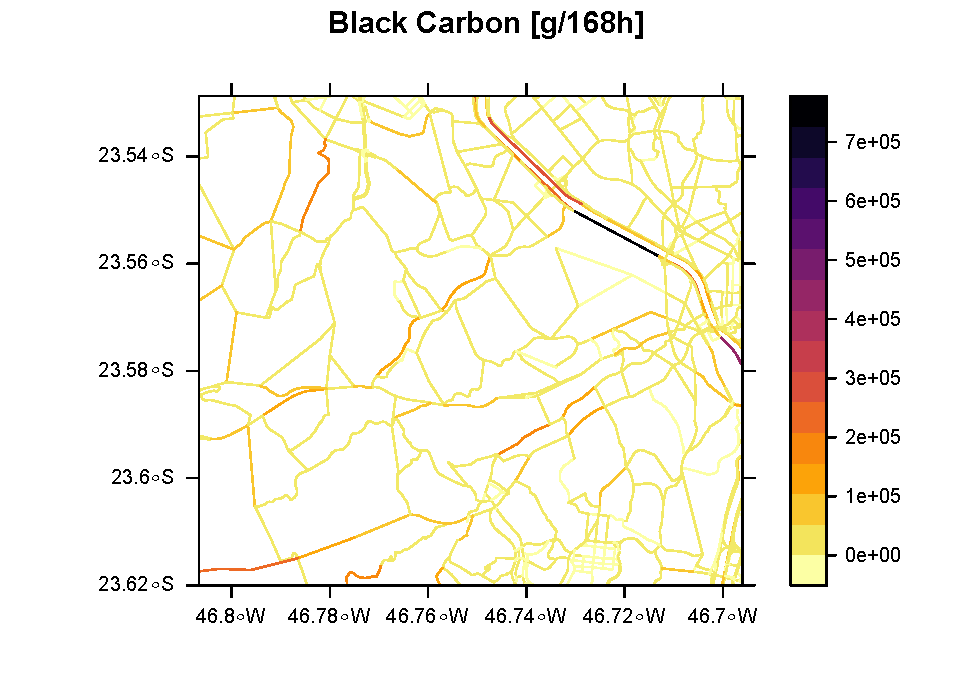
\includegraphics{veinbook_files/figure-latex/spplotbm-1.pdf}
\caption{\label{fig:spplotbm}Black Carbon {[}g/168h{]}}
\end{figure}

and Organic Matter

\begin{Shaded}
\begin{Highlighting}[]
\NormalTok{sp}\OperatorTok{::}\KeywordTok{spplot}\NormalTok{(net, }\StringTok{"OM"}\NormalTok{, }\DataTypeTok{scales =} \KeywordTok{list}\NormalTok{(}\DataTypeTok{draw =}\NormalTok{ T), }\DataTypeTok{main =} \StringTok{"Organic Matter [g/168h]"}\NormalTok{,}
           \DataTypeTok{col.regions =} \KeywordTok{rev}\NormalTok{(cptcity}\OperatorTok{::}\KeywordTok{cpt}\NormalTok{()))}
\end{Highlighting}
\end{Shaded}

\begin{figure}
\centering
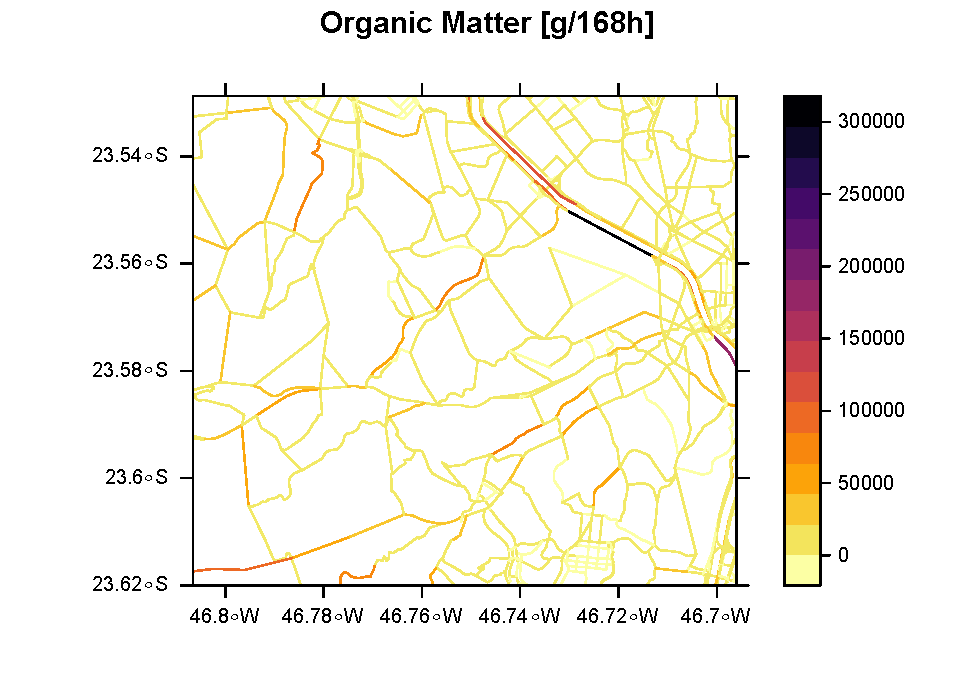
\includegraphics{veinbook_files/figure-latex/spplotom-1.pdf}
\caption{\label{fig:spplotom}Organic Matter {[}g/168h{]}}
\end{figure}

If you are interested in speciate total emissions by age of use not
spatial emissions, you could use \texttt{emis\_post} with
\texttt{by\ =\ "veh"} and then aggregate the emissions by standard. Then
speciate PM by standard:

\begin{Shaded}
\begin{Highlighting}[]
\NormalTok{dfpm <-}\StringTok{ }\KeywordTok{emis_post}\NormalTok{(}\DataTypeTok{arra =}\NormalTok{ pmd,  }\DataTypeTok{veh =} \StringTok{"LT"}\NormalTok{, }\DataTypeTok{size =} \StringTok{"small"}\NormalTok{, }\DataTypeTok{fuel =} \StringTok{"D"}\NormalTok{,}
                  \DataTypeTok{pollutant =} \StringTok{"PM"}\NormalTok{, }\DataTypeTok{by =} \StringTok{"veh"}\NormalTok{)}
\NormalTok{dfpm}\OperatorTok{$}\NormalTok{euro <-}\StringTok{ }\NormalTok{euro}
\NormalTok{dfpmeuro <-}\StringTok{ }\KeywordTok{aggregate}\NormalTok{(dfpm}\OperatorTok{$}\NormalTok{g, }\DataTypeTok{by =} \KeywordTok{list}\NormalTok{(dfpm}\OperatorTok{$}\NormalTok{euro), sum)}
\KeywordTok{names}\NormalTok{(dfpmeuro) <-}\StringTok{ }\KeywordTok{c}\NormalTok{(}\StringTok{"euro"}\NormalTok{, }\StringTok{"g"}\NormalTok{)}
\NormalTok{bcom <-}\StringTok{ }\KeywordTok{as.data.frame}\NormalTok{(}\KeywordTok{sapply}\NormalTok{(}\DecValTok{1}\OperatorTok{:}\DecValTok{6}\NormalTok{, }\ControlFlowTok{function}\NormalTok{(i)\{}
  \KeywordTok{speciate}\NormalTok{(dfpmeuro}\OperatorTok{$}\NormalTok{g[i], }\StringTok{"bcom"}\NormalTok{, }\StringTok{"PC"}\NormalTok{, }\StringTok{"D"}\NormalTok{, dfpmeuro}\OperatorTok{$}\NormalTok{euro[i])}
\NormalTok{\}))}
\KeywordTok{names}\NormalTok{(bcom) <-}\StringTok{ }\NormalTok{dfpmeuro}\OperatorTok{$}\NormalTok{euro}
\end{Highlighting}
\end{Shaded}

And the resulting speciation is:

\begin{table}

\caption{\label{tab:unnamed-chunk-84}Black Carbon and Organic Matter [g/168h]}
\centering
\begin{tabular}[t]{l|l|l|l|l|l|l}
\hline
  & I & II & III & IV & PRE & V\\
\hline
BC & 6826527.37503195 & 5313757.92745243 & 3321183.01325297 & 155078.69338865 & 6700527.80930883 & 10369.2555188646\\
\hline
OM & 2730610.95001278 & 1222164.32331406 & 498177.451987945 & 20160.2301405245 & 4690369.46651618 & 20738.5110377293\\
\hline
\end{tabular}
\end{table}

\section{Tyre wear, breaks wear and road
abrassion}\label{tyre-wear-breaks-wear-and-road-abrassion}

Tyre, break and road abrassions comes from
\citet{NtziachristosBoulter2009}. Tyres consist in a complex mixture of
rubber, which after the use starts to degradate. In deed, when the
driving cycle ismore aggresive, higher is tyre mass emitted from tyre,
with tyre wear emission factors higher in HDV than LDV. Break wear emits
mass and with more aggresive driving, more emissions.

The input are wear emissions in Total Suspended Particles (TSP) ,as
explained in section @ref(\#ew). The speciation consists in 60\% PM10,
42\% PM2.5, 6\% PM1 and 4.8\% PM0.1. Now, a simple example for TP
adspeciation:

\begin{Shaded}
\begin{Highlighting}[]
\KeywordTok{library}\NormalTok{(vein)}
\KeywordTok{data}\NormalTok{(net)}
\KeywordTok{data}\NormalTok{(profiles)}
\NormalTok{pro <-}\StringTok{ }\NormalTok{profiles}\OperatorTok{$}\NormalTok{PC_JUNE_}\DecValTok{2012}\NormalTok{[, }\DecValTok{1}\NormalTok{] }\CommentTok{# 24 hours}
\NormalTok{pc_week <-}\StringTok{ }\KeywordTok{temp_fact}\NormalTok{(net}\OperatorTok{$}\NormalTok{ldv}\OperatorTok{+}\NormalTok{net}\OperatorTok{$}\NormalTok{hdv, pro)}
\NormalTok{df <-}\StringTok{ }\KeywordTok{netspeed}\NormalTok{(pc_week, net}\OperatorTok{$}\NormalTok{ps, net}\OperatorTok{$}\NormalTok{ffs, net}\OperatorTok{$}\NormalTok{capacity, net}\OperatorTok{$}\NormalTok{lkm, }\DataTypeTok{alpha =} \DecValTok{1}\NormalTok{)}
\NormalTok{ef <-}\StringTok{ }\KeywordTok{ef_wear}\NormalTok{(}\DataTypeTok{wear =} \StringTok{"tyre"}\NormalTok{, }\DataTypeTok{type =} \StringTok{"PC"}\NormalTok{, }\DataTypeTok{speed =}\NormalTok{ df)}
\NormalTok{emit <-}\StringTok{ }\KeywordTok{emis_wear}\NormalTok{(}\DataTypeTok{veh =} \KeywordTok{age_ldv}\NormalTok{(net}\OperatorTok{$}\NormalTok{ldv, }\DataTypeTok{name =} \StringTok{"VEH"}\NormalTok{), }\DataTypeTok{speed =}\NormalTok{ df,}
                  \DataTypeTok{lkm =}\NormalTok{ net}\OperatorTok{$}\NormalTok{lkm, }\DataTypeTok{ef =}\NormalTok{ ef, }\DataTypeTok{profile =}\NormalTok{  pro)}
\end{Highlighting}
\end{Shaded}

\begin{verbatim}
## Average age of VEH is 11.17
\end{verbatim}

\begin{verbatim}
## Number of VEH is 1946.95 * 10^3 veh
\end{verbatim}

\begin{Shaded}
\begin{Highlighting}[]
\NormalTok{emib <-}\StringTok{ }\KeywordTok{emis_wear}\NormalTok{(}\DataTypeTok{what =} \StringTok{"break"}\NormalTok{, }\DataTypeTok{veh =} \KeywordTok{age_ldv}\NormalTok{(net}\OperatorTok{$}\NormalTok{ldv, }\DataTypeTok{name =} \StringTok{"VEH"}\NormalTok{),}
                  \DataTypeTok{lkm =}\NormalTok{ net}\OperatorTok{$}\NormalTok{lkm, }\DataTypeTok{ef =}\NormalTok{ ef, }\DataTypeTok{profile =}\NormalTok{  pro, }\DataTypeTok{speed =}\NormalTok{ df)}
\end{Highlighting}
\end{Shaded}

\begin{verbatim}
## Average age of VEH is 11.17
## Number of VEH is 1946.95 * 10^3 veh
\end{verbatim}

\begin{Shaded}
\begin{Highlighting}[]
\NormalTok{emit}
\end{Highlighting}
\end{Shaded}

\begin{verbatim}
## This EmissionsArray has
##  1505 streets
##  50 vehicle categories
##  24 hours
##  1 days
## [1] 0.0499920404 0.0183982869 0.0026973699 0.0066891571 0.0002749512
## [6] 0.0212774028
\end{verbatim}

\begin{Shaded}
\begin{Highlighting}[]
\NormalTok{emib}
\end{Highlighting}
\end{Shaded}

\begin{verbatim}
## This EmissionsArray has
##  1505 streets
##  50 vehicle categories
##  24 hours
##  1 days
## [1] 0.0528581237 0.0153135442 0.0022451163 0.0070774117 0.0002288516
## [6] 0.0271699850
\end{verbatim}

\begin{Shaded}
\begin{Highlighting}[]
\NormalTok{emitp <-}\StringTok{ }\KeywordTok{emis_post}\NormalTok{(}\DataTypeTok{arra =}\NormalTok{ emit, }\DataTypeTok{veh =} \StringTok{"PC"}\NormalTok{, }\DataTypeTok{size =} \StringTok{"ALL"}\NormalTok{, }\DataTypeTok{fuel =} \StringTok{"G"}\NormalTok{,}
                   \DataTypeTok{pollutant =} \StringTok{"TSP"}\NormalTok{, }\DataTypeTok{by =} \StringTok{"veh"}\NormalTok{)}
\NormalTok{emibp <-}\StringTok{ }\KeywordTok{emis_post}\NormalTok{(}\DataTypeTok{arra =}\NormalTok{ emib, }\DataTypeTok{veh =} \StringTok{"PC"}\NormalTok{, }\DataTypeTok{size =} \StringTok{"ALL"}\NormalTok{, }\DataTypeTok{fuel =} \StringTok{"G"}\NormalTok{,}
                   \DataTypeTok{pollutant =} \StringTok{"TSP"}\NormalTok{, }\DataTypeTok{by =} \StringTok{"veh"}\NormalTok{)}
\end{Highlighting}
\end{Shaded}

The estimation covered 24 hours and for simplicity, we are assuming a
year with 365 similar days and dividing by 1 million to have t/y.
Hence,the speciation is:

\begin{Shaded}
\begin{Highlighting}[]
\KeywordTok{library}\NormalTok{(ggplot2)}
\NormalTok{tyrew <-}\StringTok{ }\KeywordTok{speciate}\NormalTok{(}\DataTypeTok{x =}  \KeywordTok{unclass}\NormalTok{(emitp}\OperatorTok{$}\NormalTok{g), }\DataTypeTok{spec =} \StringTok{"tyre"}\NormalTok{)}
\NormalTok{breakw <-}\StringTok{ }\KeywordTok{speciate}\NormalTok{(}\DataTypeTok{x =}  \KeywordTok{unclass}\NormalTok{(emibp}\OperatorTok{$}\NormalTok{g), }\DataTypeTok{spec =} \StringTok{"brake"}\NormalTok{)}
\NormalTok{df <-}\StringTok{ }\KeywordTok{data.frame}\NormalTok{(}\DataTypeTok{Emis =} \KeywordTok{c}\NormalTok{(}\KeywordTok{sapply}\NormalTok{(tyrew, sum), }\KeywordTok{sapply}\NormalTok{(breakw, sum))}\OperatorTok{*}\DecValTok{365}\OperatorTok{/}\DecValTok{1000000}\NormalTok{)}
\NormalTok{df}\OperatorTok{$}\NormalTok{Pollutant <-}\StringTok{ }\KeywordTok{factor}\NormalTok{(}\DataTypeTok{x =} \KeywordTok{names}\NormalTok{(tyrew), }\DataTypeTok{levels =} \KeywordTok{names}\NormalTok{(tyrew))}
\NormalTok{df}\OperatorTok{$}\NormalTok{Emissions <-}\StringTok{ }\KeywordTok{c}\NormalTok{(}\KeywordTok{rep}\NormalTok{(}\StringTok{"Tyre"}\NormalTok{, }\DecValTok{4}\NormalTok{), }\KeywordTok{rep}\NormalTok{(}\StringTok{"Brake"}\NormalTok{, }\DecValTok{4}\NormalTok{))}
\KeywordTok{ggplot}\NormalTok{(df, }\KeywordTok{aes}\NormalTok{(}\DataTypeTok{x =}\NormalTok{ Pollutant, }\DataTypeTok{y =}\NormalTok{ Emis, }\DataTypeTok{fill =}\NormalTok{ Emissions)) }\OperatorTok{+}
\StringTok{  }\KeywordTok{geom_bar}\NormalTok{(}\DataTypeTok{stat =} \StringTok{"identity"}\NormalTok{, }\DataTypeTok{position =} \StringTok{"dodge"}\NormalTok{)}\OperatorTok{+}
\StringTok{  }\KeywordTok{labs}\NormalTok{(}\DataTypeTok{x =} \OtherTok{NULL}\NormalTok{, }\DataTypeTok{y =} \StringTok{"[t/y]"}\NormalTok{)}
\end{Highlighting}
\end{Shaded}

\begin{figure}
\centering
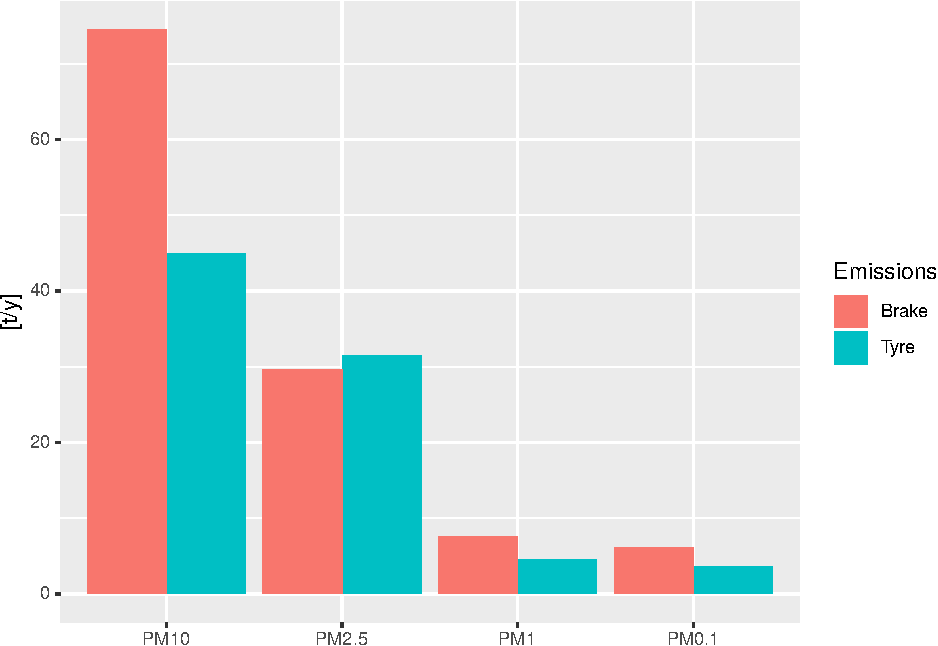
\includegraphics{veinbook_files/figure-latex/styre-1.pdf}
\caption{\label{fig:styre}Break and Tyre emissions (t/y)}
\end{figure}

It is interesting to see that break emissions are higher than tyre wear
emissions, and the smalle the diameter, higher the difference, as shows:

\begin{table}

\caption{\label{tab:unnamed-chunk-86}Ratio between break and tyre wear emissions}
\centering
\begin{tabular}[t]{l|r}
\hline
  & x\\
\hline
PM10 & 1.6593167\\
\hline
PM2.5 & 0.9433433\\
\hline
PM1 & 1.6931803\\
\hline
PM0.1 & 1.6931803\\
\hline
\end{tabular}
\end{table}

The procudure can be used with \texttt{emis\_post} with
\texttt{by\ \ =\ streets\_wide} to obtain the spatial speciation.

\section{\texorpdfstring{\(NO\) and
\(NO_2\)}{NO and NO\_2}}\label{no-and-no_2}

The speciation of \(NO_X\) into \(NO\) and \(NO2\) depends on the type
of vehicle, fuel and euro standard. The following example will consists
in comparing a Gasoline passenger car and a Diesel truck.

\begin{Shaded}
\begin{Highlighting}[]
\KeywordTok{library}\NormalTok{(vein)}
\KeywordTok{data}\NormalTok{(net)}
\KeywordTok{data}\NormalTok{(profiles)}
\NormalTok{propc <-}\StringTok{ }\NormalTok{profiles}\OperatorTok{$}\NormalTok{PC_JUNE_}\DecValTok{2012}\NormalTok{[, }\DecValTok{1}\NormalTok{] }\CommentTok{# 24 hours}
\NormalTok{prolt <-}\StringTok{ }\NormalTok{profiles}\OperatorTok{$}\NormalTok{PC_JUNE_}\DecValTok{2012}\NormalTok{[, }\DecValTok{1}\NormalTok{] }\CommentTok{# 24 hours}
\NormalTok{pweek <-}\StringTok{ }\KeywordTok{temp_fact}\NormalTok{(net}\OperatorTok{$}\NormalTok{ldv}\OperatorTok{+}\NormalTok{net}\OperatorTok{$}\NormalTok{hdv, pro)}
\NormalTok{df <-}\StringTok{ }\KeywordTok{netspeed}\NormalTok{(pc_week, net}\OperatorTok{$}\NormalTok{ps, net}\OperatorTok{$}\NormalTok{ffs, net}\OperatorTok{$}\NormalTok{capacity, net}\OperatorTok{$}\NormalTok{lkm, }\DataTypeTok{alpha =} \DecValTok{1}\NormalTok{)}
\NormalTok{euro <-}\StringTok{ }\KeywordTok{c}\NormalTok{(}\StringTok{"V"}\NormalTok{, }\KeywordTok{rep}\NormalTok{(}\StringTok{"IV"}\NormalTok{, }\DecValTok{3}\NormalTok{),  }
          \KeywordTok{rep}\NormalTok{(}\StringTok{"III"}\NormalTok{, }\DecValTok{7}\NormalTok{), }\KeywordTok{rep}\NormalTok{(}\StringTok{"II"}\NormalTok{, }\DecValTok{7}\NormalTok{), }\KeywordTok{rep}\NormalTok{(}\StringTok{"I"}\NormalTok{, }\DecValTok{5}\NormalTok{), }\KeywordTok{rep}\NormalTok{(}\StringTok{"PRE"}\NormalTok{, }\DecValTok{27}\NormalTok{))}
\NormalTok{lefpc <-}\StringTok{ }\KeywordTok{lapply}\NormalTok{(}\DecValTok{1}\OperatorTok{:}\DecValTok{50}\NormalTok{, }\ControlFlowTok{function}\NormalTok{(i) \{}
  \KeywordTok{ef_ldv_speed}\NormalTok{(}\DataTypeTok{v =} \StringTok{"PC"}\NormalTok{, }\DataTypeTok{t =} \StringTok{"4S"}\NormalTok{, }\DataTypeTok{cc =} \StringTok{"<=1400"}\NormalTok{, }\DataTypeTok{f =} \StringTok{"G"}\NormalTok{,}
               \DataTypeTok{eu =}\NormalTok{ euro[i], }\DataTypeTok{p =} \StringTok{"NOx"}\NormalTok{, }\DataTypeTok{show.equation =} \OtherTok{FALSE}\NormalTok{) \})}
\NormalTok{leflt <-}\StringTok{ }\KeywordTok{lapply}\NormalTok{(}\DecValTok{1}\OperatorTok{:}\DecValTok{50}\NormalTok{, }\ControlFlowTok{function}\NormalTok{(i) \{}
  \KeywordTok{ef_hdv_speed}\NormalTok{(}\DataTypeTok{v =} \StringTok{"Trucks"}\NormalTok{, }\DataTypeTok{t =} \StringTok{"RT"}\NormalTok{, }\DataTypeTok{g =} \StringTok{">32"}\NormalTok{, }\DataTypeTok{gr =} \DecValTok{0}\NormalTok{,}
               \DataTypeTok{eu =}\NormalTok{ euro[i], }\DataTypeTok{l =} \FloatTok{0.5}\NormalTok{, }\DataTypeTok{p =} \StringTok{"NOx"}\NormalTok{, }\DataTypeTok{show.equation =} \OtherTok{FALSE}\NormalTok{) \})}
\NormalTok{emipc <-}\StringTok{ }\KeywordTok{emis}\NormalTok{(}\DataTypeTok{veh =} \KeywordTok{age_ldv}\NormalTok{(net}\OperatorTok{$}\NormalTok{ldv),}\DataTypeTok{lkm =}\NormalTok{ net}\OperatorTok{$}\NormalTok{lkm, }\DataTypeTok{ef =}\NormalTok{ lefpc, }\DataTypeTok{speed =}\NormalTok{ df,}
              \DataTypeTok{profile =}\NormalTok{ profiles}\OperatorTok{$}\NormalTok{PC_JUNE_}\DecValTok{2014}\NormalTok{[, }\DecValTok{1}\NormalTok{])}\OperatorTok{*}\DecValTok{365}\OperatorTok{/}\DecValTok{1000000}
\end{Highlighting}
\end{Shaded}

\begin{verbatim}
## Average age of age is 11.17
\end{verbatim}

\begin{verbatim}
## Number of age is 1946.95 * 10^3 veh
\end{verbatim}

\begin{verbatim}
## 4097.62 kg emissions in 24 hours and 1 days
\end{verbatim}

\begin{Shaded}
\begin{Highlighting}[]
\NormalTok{emilt <-}\StringTok{ }\KeywordTok{emis}\NormalTok{(}\DataTypeTok{veh =} \KeywordTok{age_ldv}\NormalTok{(net}\OperatorTok{$}\NormalTok{hdv),}\DataTypeTok{lkm =}\NormalTok{ net}\OperatorTok{$}\NormalTok{lkm, }\DataTypeTok{ef =}\NormalTok{ leflt, }\DataTypeTok{speed =}\NormalTok{ df,}
              \DataTypeTok{profile =}\NormalTok{ profiles}\OperatorTok{$}\NormalTok{HGV_JUNE_}\DecValTok{2014}\NormalTok{[, }\DecValTok{1}\NormalTok{])}\OperatorTok{*}\DecValTok{365}\OperatorTok{/}\DecValTok{1000000}
\end{Highlighting}
\end{Shaded}

\begin{verbatim}
## Average age of age is 11.17
\end{verbatim}

\begin{verbatim}
## Number of age is 148.12 * 10^3 veh
\end{verbatim}

\begin{verbatim}
## 14612.67 kg emissions in 24 hours and 1 days
\end{verbatim}

Then, once the emissions are estimated, we will speciate the emissions
by euro standard. The estimation covered 24 hours and for simplicity, we
are assuming a year with 365 similar days and dividing by 1 million to
have t/y.

\begin{Shaded}
\begin{Highlighting}[]
\NormalTok{df <-}\StringTok{ }\KeywordTok{rowSums}\NormalTok{(}\KeywordTok{apply}\NormalTok{(}\DataTypeTok{X =}\NormalTok{ emipc, }\DataTypeTok{MARGIN =} \KeywordTok{c}\NormalTok{(}\DecValTok{2}\NormalTok{,}\DecValTok{3}\NormalTok{), }\DataTypeTok{FUN =}\NormalTok{ sum, }\DataTypeTok{na.rm =} \OtherTok{TRUE}\NormalTok{))}
\NormalTok{dfpc <-}\StringTok{   }\KeywordTok{rbind}\NormalTok{(}\KeywordTok{speciate}\NormalTok{(df[}\DecValTok{1}\NormalTok{], }\StringTok{"nox"}\NormalTok{, }\StringTok{"PC"}\NormalTok{, }\StringTok{"G"}\NormalTok{, }\StringTok{"V"}\NormalTok{),}
                \KeywordTok{speciate}\NormalTok{(df[}\DecValTok{2}\OperatorTok{:}\DecValTok{4}\NormalTok{], }\StringTok{"nox"}\NormalTok{, }\StringTok{"PC"}\NormalTok{, }\StringTok{"G"}\NormalTok{, }\StringTok{"V"}\NormalTok{),}
                \KeywordTok{speciate}\NormalTok{(df[}\DecValTok{5}\OperatorTok{:}\DecValTok{11}\NormalTok{], }\StringTok{"nox"}\NormalTok{, }\StringTok{"PC"}\NormalTok{, }\StringTok{"G"}\NormalTok{, }\StringTok{"V"}\NormalTok{),}
                \KeywordTok{speciate}\NormalTok{(df[}\DecValTok{12}\OperatorTok{:}\DecValTok{18}\NormalTok{], }\StringTok{"nox"}\NormalTok{, }\StringTok{"PC"}\NormalTok{, }\StringTok{"G"}\NormalTok{, }\StringTok{"V"}\NormalTok{),}
                \KeywordTok{speciate}\NormalTok{(df[}\DecValTok{19}\OperatorTok{:}\DecValTok{23}\NormalTok{], }\StringTok{"nox"}\NormalTok{, }\StringTok{"PC"}\NormalTok{, }\StringTok{"G"}\NormalTok{, }\StringTok{"V"}\NormalTok{),}
                \KeywordTok{speciate}\NormalTok{(df[}\DecValTok{24}\OperatorTok{:}\DecValTok{50}\NormalTok{], }\StringTok{"nox"}\NormalTok{, }\StringTok{"PC"}\NormalTok{, }\StringTok{"G"}\NormalTok{, }\StringTok{"V"}\NormalTok{))}
\NormalTok{df <-}\StringTok{ }\KeywordTok{rowSums}\NormalTok{(}\KeywordTok{apply}\NormalTok{(}\DataTypeTok{X =}\NormalTok{ emipc, }\DataTypeTok{MARGIN =} \KeywordTok{c}\NormalTok{(}\DecValTok{2}\NormalTok{,}\DecValTok{3}\NormalTok{), }\DataTypeTok{FUN =}\NormalTok{ sum, }\DataTypeTok{na.rm =} \OtherTok{TRUE}\NormalTok{))}
\NormalTok{dfhdv <-}\StringTok{   }\KeywordTok{rbind}\NormalTok{(}\KeywordTok{speciate}\NormalTok{(df[}\DecValTok{1}\NormalTok{], }\StringTok{"nox"}\NormalTok{, }\StringTok{"HDV"}\NormalTok{, }\StringTok{"D"}\NormalTok{, }\StringTok{"V"}\NormalTok{),}
                 \KeywordTok{speciate}\NormalTok{(df[}\DecValTok{2}\OperatorTok{:}\DecValTok{4}\NormalTok{], }\StringTok{"nox"}\NormalTok{, }\StringTok{"HDV"}\NormalTok{, }\StringTok{"D"}\NormalTok{, }\StringTok{"V"}\NormalTok{),}
                 \KeywordTok{speciate}\NormalTok{(df[}\DecValTok{5}\OperatorTok{:}\DecValTok{11}\NormalTok{], }\StringTok{"nox"}\NormalTok{, }\StringTok{"HDV"}\NormalTok{, }\StringTok{"D"}\NormalTok{, }\StringTok{"V"}\NormalTok{),}
                 \KeywordTok{speciate}\NormalTok{(df[}\DecValTok{12}\OperatorTok{:}\DecValTok{18}\NormalTok{], }\StringTok{"nox"}\NormalTok{, }\StringTok{"HDV"}\NormalTok{, }\StringTok{"D"}\NormalTok{, }\StringTok{"V"}\NormalTok{),}
                 \KeywordTok{speciate}\NormalTok{(df[}\DecValTok{19}\OperatorTok{:}\DecValTok{23}\NormalTok{], }\StringTok{"nox"}\NormalTok{, }\StringTok{"HDV"}\NormalTok{, }\StringTok{"D"}\NormalTok{, }\StringTok{"V"}\NormalTok{),}
                 \KeywordTok{speciate}\NormalTok{(df[}\DecValTok{24}\OperatorTok{:}\DecValTok{50}\NormalTok{], }\StringTok{"nox"}\NormalTok{, }\StringTok{"HDV"}\NormalTok{, }\StringTok{"D"}\NormalTok{, }\StringTok{"V"}\NormalTok{))}

\NormalTok{df <-}\StringTok{ }\KeywordTok{data.frame}\NormalTok{(}\KeywordTok{rbind}\NormalTok{(}\KeywordTok{sapply}\NormalTok{(dfpc, sum), }\KeywordTok{sapply}\NormalTok{(dfhdv, sum)))}
\KeywordTok{row.names}\NormalTok{(df) <-}\StringTok{ }\KeywordTok{c}\NormalTok{(}\StringTok{"PC"}\NormalTok{, }\StringTok{"HGV"}\NormalTok{)}
\NormalTok{knitr}\OperatorTok{::}\KeywordTok{kable}\NormalTok{(df, }\DataTypeTok{caption =} \StringTok{"NO2 and NO speciation (t/y)"}\NormalTok{)}
\end{Highlighting}
\end{Shaded}

\begin{table}

\caption{\label{tab:sno2}NO2 and NO speciation (t/y)}
\centering
\begin{tabular}[t]{l|r|r}
\hline
  & NO2 & NO\\
\hline
PC & 44.8689 & 1450.761\\
\hline
HGV & 179.4756 & 1316.154\\
\hline
\end{tabular}
\end{table}

\section{\texorpdfstring{Volatile organic compounds:
\texttt{nmhc}}{Volatile organic compounds: nmhc}}\label{volatile-organic-compounds-nmhc}

nmhc were shown earluier in this chapter, but they can be also used to
speciate objects, resulting in all species at once. The speciation of
NMHC must be applied to NMHC. However, the emission guidelines of
\citet{NtziachristosSamaras2016} does not show explicit emission factor
of NMHC and the suggeted procedure is substract the \(CH_4\) from the
\(HC\). This was done on VEIN and now, ef\_speed* functions returns NMHC
directly. This makes easier to produce speciation.

\begin{Shaded}
\begin{Highlighting}[]
\KeywordTok{library}\NormalTok{(vein)}
\KeywordTok{data}\NormalTok{(net)}
\KeywordTok{data}\NormalTok{(profiles)}
\NormalTok{propc <-}\StringTok{ }\NormalTok{profiles}\OperatorTok{$}\NormalTok{PC_JUNE_}\DecValTok{2012}\NormalTok{[, }\DecValTok{1}\NormalTok{] }\CommentTok{# 24 hours}
\NormalTok{pweek <-}\StringTok{ }\KeywordTok{temp_fact}\NormalTok{(net}\OperatorTok{$}\NormalTok{ldv}\OperatorTok{+}\NormalTok{net}\OperatorTok{$}\NormalTok{hdv, propc)}
\NormalTok{df <-}\StringTok{ }\KeywordTok{netspeed}\NormalTok{(pweek, net}\OperatorTok{$}\NormalTok{ps, net}\OperatorTok{$}\NormalTok{ffs, net}\OperatorTok{$}\NormalTok{capacity, net}\OperatorTok{$}\NormalTok{lkm, }\DataTypeTok{alpha =} \DecValTok{1}\NormalTok{)}
\NormalTok{euro <-}\StringTok{ }\KeywordTok{c}\NormalTok{(}\StringTok{"V"}\NormalTok{, }\KeywordTok{rep}\NormalTok{(}\StringTok{"IV"}\NormalTok{, }\DecValTok{3}\NormalTok{),  }
          \KeywordTok{rep}\NormalTok{(}\StringTok{"III"}\NormalTok{, }\DecValTok{7}\NormalTok{), }\KeywordTok{rep}\NormalTok{(}\StringTok{"II"}\NormalTok{, }\DecValTok{7}\NormalTok{), }\KeywordTok{rep}\NormalTok{(}\StringTok{"I"}\NormalTok{, }\DecValTok{5}\NormalTok{), }\KeywordTok{rep}\NormalTok{(}\StringTok{"PRE"}\NormalTok{, }\DecValTok{27}\NormalTok{))}
\NormalTok{lefpc <-}\StringTok{ }\KeywordTok{lapply}\NormalTok{(}\DecValTok{1}\OperatorTok{:}\DecValTok{50}\NormalTok{, }\ControlFlowTok{function}\NormalTok{(i) \{}
  \KeywordTok{ef_ldv_speed}\NormalTok{(}\DataTypeTok{v =} \StringTok{"PC"}\NormalTok{, }\DataTypeTok{t =} \StringTok{"4S"}\NormalTok{, }\DataTypeTok{cc =} \StringTok{"<=1400"}\NormalTok{, }\DataTypeTok{f =} \StringTok{"G"}\NormalTok{,}
               \DataTypeTok{eu =}\NormalTok{ euro[i], }\DataTypeTok{p =} \StringTok{"NMHC"}\NormalTok{, }\DataTypeTok{show.equation =} \OtherTok{FALSE}\NormalTok{)\})}
\end{Highlighting}
\end{Shaded}

\begin{Shaded}
\begin{Highlighting}[]
\NormalTok{euro <-}\StringTok{ }\KeywordTok{c}\NormalTok{(}\StringTok{"V"}\NormalTok{, }\KeywordTok{rep}\NormalTok{(}\StringTok{"IV"}\NormalTok{, }\DecValTok{3}\NormalTok{),  }
          \KeywordTok{rep}\NormalTok{(}\StringTok{"III"}\NormalTok{, }\DecValTok{7}\NormalTok{), }\KeywordTok{rep}\NormalTok{(}\StringTok{"II"}\NormalTok{, }\DecValTok{7}\NormalTok{), }\KeywordTok{rep}\NormalTok{(}\StringTok{"I"}\NormalTok{, }\DecValTok{5}\NormalTok{), }\KeywordTok{rep}\NormalTok{(}\StringTok{"PRE"}\NormalTok{, }\DecValTok{27}\NormalTok{))}
\NormalTok{lefpc <-}\StringTok{ }\KeywordTok{lapply}\NormalTok{(}\DecValTok{1}\OperatorTok{:}\KeywordTok{length}\NormalTok{(euro), }\ControlFlowTok{function}\NormalTok{(i) \{}
  \KeywordTok{ef_ldv_speed}\NormalTok{(}\DataTypeTok{v =} \StringTok{"PC"}\NormalTok{, }\DataTypeTok{t =} \StringTok{"4S"}\NormalTok{, }\DataTypeTok{cc =} \StringTok{"<=1400"}\NormalTok{, }\DataTypeTok{f =} \StringTok{"G"}\NormalTok{,}
               \DataTypeTok{eu =}\NormalTok{ euro[i], }\DataTypeTok{p =} \StringTok{"HC"}\NormalTok{, }\DataTypeTok{show.equation =} \OtherTok{FALSE}\NormalTok{) \})}
\NormalTok{enmhc <-}\StringTok{ }\KeywordTok{emis}\NormalTok{(}\DataTypeTok{veh =} \KeywordTok{age_ldv}\NormalTok{(net}\OperatorTok{$}\NormalTok{ldv), }\DataTypeTok{lkm =}\NormalTok{ net}\OperatorTok{$}\NormalTok{lkm, }\DataTypeTok{ef =}\NormalTok{ lefpc, }\DataTypeTok{speed =}\NormalTok{ df,}
              \DataTypeTok{profile =}\NormalTok{ profiles}\OperatorTok{$}\NormalTok{PC_JUNE_}\DecValTok{2014}\NormalTok{[, }\DecValTok{1}\NormalTok{])}
\end{Highlighting}
\end{Shaded}

\begin{verbatim}
## Average age of age is 11.17
\end{verbatim}

\begin{verbatim}
## Number of age is 1946.95 * 10^3 veh
\end{verbatim}

\begin{verbatim}
## 3030.65 kg emissions in 24 hours and 1 days
\end{verbatim}

\begin{Shaded}
\begin{Highlighting}[]
\NormalTok{df_enmhc <-}\StringTok{ }\KeywordTok{emis_post}\NormalTok{(}\DataTypeTok{arra =}\NormalTok{ enmhc, }\DataTypeTok{veh =} \StringTok{"PC"}\NormalTok{, }\DataTypeTok{size =} \StringTok{"ALL"}\NormalTok{, }\DataTypeTok{fuel =} \StringTok{"G"}\NormalTok{,}
                      \DataTypeTok{pollutant =} \StringTok{"NMHC"}\NormalTok{, }\DataTypeTok{by =} \StringTok{"veh"}\NormalTok{)}
\CommentTok{# assuming all euro I}
\NormalTok{spec <-}\StringTok{ }\KeywordTok{speciate}\NormalTok{(}\DataTypeTok{x =} \KeywordTok{as.numeric}\NormalTok{(df_enmhc}\OperatorTok{$}\NormalTok{g), }\DataTypeTok{spec =} \StringTok{"nmhc"}\NormalTok{, }\DataTypeTok{veh =} \StringTok{"LDV"}\NormalTok{,}
                 \DataTypeTok{fuel =} \StringTok{"G"}\NormalTok{, }\DataTypeTok{eu =} \StringTok{"I"}\NormalTok{)}
\KeywordTok{names}\NormalTok{(spec)}
\end{Highlighting}
\end{Shaded}

\begin{verbatim}
##  [1] "ethane"                   "propane"                 
##  [3] "butane"                   "isobutane"               
##  [5] "pentane"                  "isopentane"              
##  [7] "hexane"                   "heptane"                 
##  [9] "octane"                   "TWO_methylhexane"        
## [11] "nonane"                   "TWO_methylheptane"       
## [13] "THREE_methylhexane"       "decane"                  
## [15] "THREE_methylheptane"      "alcanes_C10_C12"         
## [17] "alkanes_C13"              "cycloalcanes"            
## [19] "ethylene"                 "propylene"               
## [21] "propadiene"               "ONE_butene"              
## [23] "isobutene"                "TWO_butene"              
## [25] "ONE_3_butadiene"          "ONE_pentene"             
## [27] "TWO_pentene"              "ONE_hexene"              
## [29] "dimethylhexene"           "ONE_butine"              
## [31] "propine"                  "acetylene"               
## [33] "formaldehyde"             "acetaldehyde"            
## [35] "acrolein"                 "benzaldehyde"            
## [37] "crotonaldehyde"           "methacrolein"            
## [39] "butyraldehyde"            "isobutanaldehyde"        
## [41] "propionaldehyde"          "hexanal"                 
## [43] "i_valeraldehyde"          "valeraldehyde"           
## [45] "o_tolualdehyde"           "m_tolualdehyde"          
## [47] "p_tolualdehyde"           "acetone"                 
## [49] "methylethlketone"         "toluene"                 
## [51] "ethylbenzene"             "m_p_xylene"              
## [53] "o_xylene"                 "ONE_2_3_trimethylbenzene"
## [55] "ONE_2_4_trimethylbenzene" "ONE_3_5_trimethylbenzene"
## [57] "styrene"                  "benzene"                 
## [59] "C9"                       "C10"                     
## [61] "C13"
\end{verbatim}

\section{\texorpdfstring{The speciation
\texttt{iag}}{The speciation iag}}\label{the-speciation-iag}

The Carbon Bond Mechanism Z \citeyearpar{cbmz} is an lumped-structure
mechanism.

Citing:

**``it is currently unfeasible to treat the organic species individually
in a regional or global chemistry model for three major reasons:**

\textbf{- (1) limited computational resources,} \textbf{- (2) lack of
detailed speciated emissions inventories, and } \textbf{- (3) lack of
kinetic and mechanistic information for all the species and their
reaction products.}

\textbf{Thus there exists a need for a condensed mechanism that is
capable of describing the tropospheric hydrocarbon chemistry with
reasonable accuracy, sensitivity, and speed at regional to global
scales. }

The research in this aspect is intense and out of the scope of this
book. However, it is important that the user who intends to performs
atmospheric simulation to understand this why it is important to
speciate the emissions and what represent each group.

A popular air quality model nowedays is the Weather Research and
Forecasting model coupled to Chemistry (WRF-Chem) \citep{Grelletal2005}
\url{https://ruc.noaa.gov/wrf/wrf-chem/and} the \textbf{Emissions Guide}
(\url{https://ruc.noaa.gov/wrf/wrf-chem/Emission_guide.pdf}).

The speciation \texttt{iag} splits the NMHC into the lumped groups for
the mechanism CMB-Z. The name \texttt{iag} comes from the Institute of
Astronomy, Geophysics and Atmospheric Sciences (IAG,
\url{http://www.iag.usp.br/}) from the University of São Paulo (USP).
The Departament of Atmospheric Sciences (DAC) of IAG has measure and
model air quality models for several years. There are several scientific
production such as: \citet{Nogueiraetal2015},
\citet{HOSHYARIPOUR2016365}, \citet{Andradeetal2017},
\citet{Freitasetal2005}, \citet{martins2006emission},
\citet{perez2014emission}, \citet{ulke2001modeling},
\citet{vivanco2006validation}, \citet{boian2012characterization},
\citet{Andrade2012}, \citet{Andradeetal2015}, \citet{VaraVelaetal2015},
\citet{Rafee2015}, \citet{Ibarraetal2017b}. The following figure, shows
an air quality simulation over South Easth Brazil from DAC/IAG/USP.

\begin{figure}
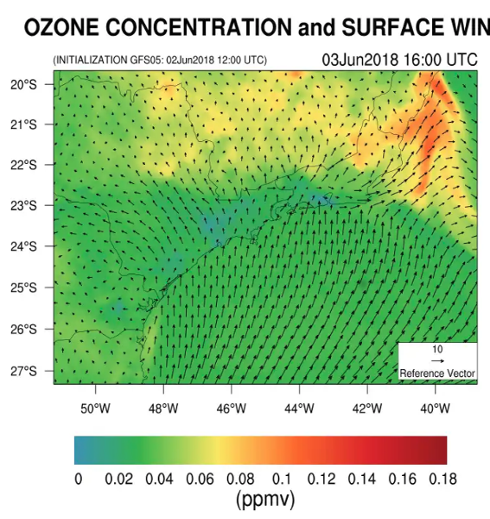
\includegraphics[width=6.81in]{figuras/wrf} \caption{http://www.lapat.iag.usp.br/aerossol/wrf9/index.php}\label{fig:unnamed-chunk-90}
\end{figure}

Some of these papers show measurements in tunnels, fuel, etc. The
speciation \texttt{iag} it is based on these experiments, and the last
versions, covers an update during 2015 so that the exhaust emissions
speciation is more representative of brazilian gasoline. This means
that:

\begin{itemize}
\tightlist
\item
  ** THE SPECIATION \texttt{IAG} IS BASED ON BRAZILIAN MEASUREMENTS**.
\end{itemize}

and the user who wants to applt it outside Brazil, should be ensure,
that the fleet and fuel are compatible. As that will be hard to
accomplish, I can say that this speciation is for and to be used in
Brazil, even more, in São Paulo.

The currently speciation \texttt{iag} is:

\begin{figure}
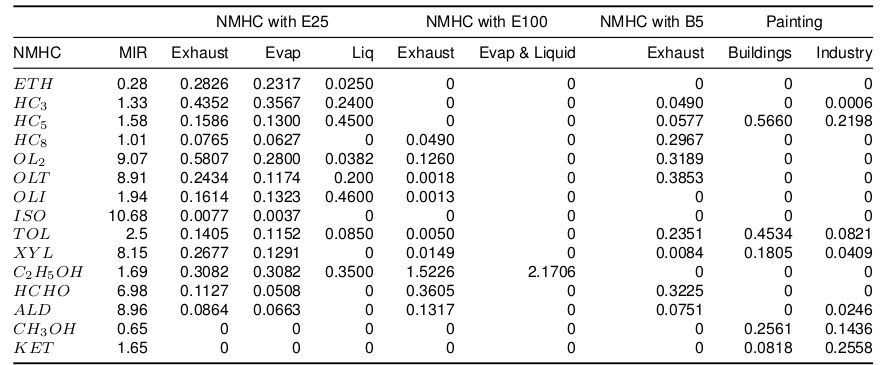
\includegraphics[width=12.36in]{figuras/iag1} \caption{Speciation for NMHC by type of fuel and process mol/100g (Ibarra-Espinosa, S., 2017)}\label{fig:unnamed-chunk-91}
\end{figure}

The arguments of the function \texttt{speciate} take the following form:

\begin{itemize}
\tightlist
\item
  \texttt{x}: Emissions estimation, it is recommended that x are
  griddded emissions from NMHC.
\item
  \texttt{spec}: \texttt{iag}. Alternatively, you can put any name of
  the following: ``e\_eth'', ``e\_hc3'', ``e\_hc5'', ``e\_hc8'',
  ``e\_ol2'', ``e\_olt'', ``e\_oli'', ``e\_iso'', ``e\_tol'',
  ``e\_xyl'', ``e\_c2h5oh'', ``e\_hcho'', ``e\_ch3oh'', ``e\_ket''
\item
  \texttt{veh}: When spec is ``iag'' veh can take two values depending:
  when the speciation is for vehicles veh accepts ``veh'', eu
  ``Evaporative'', ``Liquid'' or ``Exhaust''
\item
  \texttt{fuel}: ``G'', ``E'' or ``D''.
\item
  \texttt{eu}: ``Exhaust'' ``Evaporative'' or ``Liquid''.
\item
  \texttt{show}: Let this FALSE.
\item
  \texttt{list}: Let this TRUE so that the result is a list, and each
  element of the list a lumped specie.
\end{itemize}

Example:

\begin{Shaded}
\begin{Highlighting}[]
\CommentTok{# Do not run}
\NormalTok{x <-}\StringTok{ }\KeywordTok{data.frame}\NormalTok{(}\DataTypeTok{x =} \KeywordTok{rnorm}\NormalTok{(}\DataTypeTok{n =} \DecValTok{100}\NormalTok{, }\DataTypeTok{mean =} \DecValTok{400}\NormalTok{, }\DataTypeTok{sd =} \DecValTok{2}\NormalTok{))}
\NormalTok{dfa <-}\StringTok{ }\KeywordTok{speciate}\NormalTok{(x, }\DataTypeTok{spec =} \StringTok{"e_eth"}\NormalTok{, }\DataTypeTok{veh =} \StringTok{"veh"}\NormalTok{, }\DataTypeTok{fuel =} \StringTok{"G"}\NormalTok{, }\DataTypeTok{eu =} \StringTok{"Exhaust"}\NormalTok{)}
\KeywordTok{head}\NormalTok{(dfa)}
\end{Highlighting}
\end{Shaded}

\begin{verbatim}
##       e_eth
## 1 0.9264749
## 2 0.9209588
## 3 0.9337412
## 4 0.9243835
## 5 0.9306481
## 6 0.9242471
\end{verbatim}

\begin{Shaded}
\begin{Highlighting}[]
\NormalTok{df <-}\StringTok{ }\KeywordTok{speciate}\NormalTok{(x, }\DataTypeTok{spec =} \StringTok{"iag"}\NormalTok{, }\DataTypeTok{veh =} \StringTok{"veh"}\NormalTok{, }\DataTypeTok{fuel =} \StringTok{"G"}\NormalTok{,}
               \DataTypeTok{eu =} \StringTok{"Exhaust"}\NormalTok{, }\DataTypeTok{list =} \OtherTok{TRUE}\NormalTok{)}
\KeywordTok{names}\NormalTok{(df)}
\end{Highlighting}
\end{Shaded}

\begin{verbatim}
##  [1] "e_eth"    "e_hc3"    "e_hc5"    "e_hc8"    "e_ol2"    "e_olt"   
##  [7] "e_oli"    "e_iso"    "e_tol"    "e_xyl"    "e_c2h5oh" "e_ald"   
## [13] "e_hcho"   "e_ch3oh"  "e_ket"
\end{verbatim}

\begin{Shaded}
\begin{Highlighting}[]
\ControlFlowTok{for}\NormalTok{(i }\ControlFlowTok{in} \DecValTok{1}\OperatorTok{:}\KeywordTok{length}\NormalTok{(df))\{}
  \KeywordTok{print}\NormalTok{(df[[i]][}\DecValTok{1}\OperatorTok{:}\DecValTok{3}\NormalTok{, ]) }\CommentTok{# Firt three lines of each element of the list}
\NormalTok{\}}
\end{Highlighting}
\end{Shaded}

\begin{verbatim}
## Units: [mol/h]
## [1] 0.9264749 0.9209588 0.9337412
## Units: [mol/h]
## [1] 1.426650 1.418156 1.437839
## Units: [mol/h]
## [1] 0.5199713 0.5168755 0.5240495
## Units: [mol/h]
## [1] 0.2508993 0.2494055 0.2528671
## Units: [mol/h]
## [1] 1.903661 1.892327 1.918591
## Units: [mol/h]
## [1] 0.7980894 0.7933377 0.8043488
## Units: [mol/h]
## [1] 0.5291057 0.5259555 0.5332555
## Units: [mol/h]
## [1] 0.02537988 0.02522877 0.02557893
## Units: [mol/h]
## [1] 0.4605939 0.4578516 0.4642063
## Units: [mol/h]
## [1] 0.8775060 0.8722815 0.8843883
## Units: [mol/h]
## [1] 1.232596 1.225258 1.242264
## Units: [mol/h]
## [1] 0.3455144 0.3434573 0.3482243
## Units: [mol/h]
## [1] 0.4506237 0.4479407 0.4541579
## Units: [mol/h]
## [1] 0 0 0
## Units: [mol/h]
## [1] 0 0 0
\end{verbatim}

\section{\texorpdfstring{The speciation
\texttt{pmiag}}{The speciation pmiag}}\label{the-speciation-pmiag}

The speciation \texttt{pmiag}is also based on IAG studies and applied
only for PM2.5 emissions. The speciation splits the PM2.5 in percentages
as follow:

\begin{table}

\caption{\label{tab:unnamed-chunk-93}Speciation of PM2.5}
\centering
\begin{tabular}[t]{r|r|r|r|r|r|r|r|r|r|r}
\hline
E\_SO4i & E\_SO4j & E\_NO3i & E\_NO3j & E\_MP2.5i & E\_MP2.5j & E\_ORGi & E\_ORGj & E\_ECi & E\_ECj & H2O\\
\hline
0.0077 & 0.0623 & 0.00247 & 0.01053 & 0.1 & 0.3 & 0.0304 & 0.1296 & 0.056 & 0.024 & 0.277\\
\hline
\end{tabular}
\end{table}

When running this speciation, the only two required arguments are
\texttt{x} and \texttt{spec}. Also, There is a message that this
speciation applies \textbf{only in gridded emissions, because the unit
must be in flux \(g/km^2/h\)}, and internally are transformed to the
required unit \$ \mu g/m\^{}2/s\$ as:

\[ \frac{g}{(km)^2*h}*\frac{10^6 \mu g}{g}*(\frac{km}{1000m})^2*\frac{h}{3600s}\frac{1}{dx^2}\]

dx is the length of the grid cell. Example:

\begin{Shaded}
\begin{Highlighting}[]
\KeywordTok{library}\NormalTok{(vein)}
\KeywordTok{data}\NormalTok{(net)}
\NormalTok{pm <-}\StringTok{ }\KeywordTok{data.frame}\NormalTok{(}\DataTypeTok{pm =} \KeywordTok{rnorm}\NormalTok{(}\DataTypeTok{n =} \KeywordTok{length}\NormalTok{(net), }\DataTypeTok{mean =} \DecValTok{400}\NormalTok{, }\DataTypeTok{sd =} \DecValTok{2}\NormalTok{))}
\NormalTok{net}\OperatorTok{@}\NormalTok{data <-}\StringTok{ }\NormalTok{pm}
\NormalTok{g <-}\StringTok{ }\KeywordTok{make_grid}\NormalTok{(net, }\DecValTok{1}\OperatorTok{/}\FloatTok{102.47}\OperatorTok{/}\DecValTok{2}\NormalTok{) }\CommentTok{# 500 m}
\end{Highlighting}
\end{Shaded}

\begin{verbatim}
## Number of lon points: 23
## Number of lat points: 19
\end{verbatim}

\begin{Shaded}
\begin{Highlighting}[]
\NormalTok{gx <-}\StringTok{ }\KeywordTok{emis_grid}\NormalTok{(net, g)}
\end{Highlighting}
\end{Shaded}

\begin{verbatim}
## Sum of street emissions 601905.2
\end{verbatim}

\begin{verbatim}
## although coordinates are longitude/latitude, st_intersection assumes that they are planar
\end{verbatim}

\begin{verbatim}
## Sum of gridded emissions 601905.2
\end{verbatim}

\begin{Shaded}
\begin{Highlighting}[]
\NormalTok{df <-}\StringTok{ }\KeywordTok{speciate}\NormalTok{(gx, }\DataTypeTok{spec =} \StringTok{"pmiag"}\NormalTok{, }\DataTypeTok{veh =} \StringTok{"veh"}\NormalTok{, }\DataTypeTok{fuel =} \StringTok{"G"}\NormalTok{,}
               \DataTypeTok{eu =} \StringTok{"Exhaust"}\NormalTok{, }\DataTypeTok{list =} \OtherTok{FALSE}\NormalTok{, }\DataTypeTok{dx =} \FloatTok{0.5}\NormalTok{)}
\end{Highlighting}
\end{Shaded}

\begin{verbatim}
## To be used in emissions grid only, emissions must be in g/(Xkm^2)/h
\end{verbatim}

\begin{verbatim}
## PM.2.5-10 must be calculated as substraction of PM10-PM2.5 to enter this variable into WRF
\end{verbatim}

\begin{Shaded}
\begin{Highlighting}[]
\KeywordTok{names}\NormalTok{(df)}
\end{Highlighting}
\end{Shaded}

\begin{verbatim}
##  [1] "e_so4i"   "e_so4j"   "e_no3i"   "e_no3j"   "e_pm2.5i" "e_pm2.5j"
##  [7] "e_orgi"   "e_orgj"   "e_eci"    "e_ecj"    "h2o"
\end{verbatim}

\begin{Shaded}
\begin{Highlighting}[]
\KeywordTok{head}\NormalTok{(df)}
\end{Highlighting}
\end{Shaded}

\begin{verbatim}
##                  e_so4i     e_so4j       e_no3i      e_no3j   e_pm2.5i
## 1 0.001450505 [g/m^2/s] 0.01173591 0.0004652920 0.001983613 0.01883773
## 2 0.001441754 [g/m^2/s] 0.01166510 0.0004624846 0.001971645 0.01872407
## 3 0.001477848 [g/m^2/s] 0.01195713 0.0004740628 0.002021005 0.01919283
## 4 0.002551616 [g/m^2/s] 0.02064489 0.0008185053 0.003489417 0.03313787
## 5 0.005798116 [g/m^2/s] 0.04691203 0.0018599150 0.007929112 0.07530020
## 6 0.000000000 [g/m^2/s] 0.00000000 0.0000000000 0.000000000 0.00000000
##     e_pm2.5j      e_orgi     e_orgj      e_eci       e_ecj        h2o
## 1 0.05651320 0.005726671 0.02441370 0.01054913 0.004521056 0.05218052
## 2 0.05617222 0.005692118 0.02426640 0.01048548 0.004493778 0.05186568
## 3 0.05757848 0.005834619 0.02487390 0.01074798 0.004606278 0.05316413
## 4 0.09941360 0.010073911 0.04294668 0.01855721 0.007953088 0.09179189
## 5 0.22590061 0.022891262 0.09758906 0.04216811 0.018072049 0.20858157
## 6 0.00000000 0.000000000 0.00000000 0.00000000 0.000000000 0.00000000
\end{verbatim}

\chapter{Inputs for atmospheric models}\label{ep}

This last chapter of this book is about generating inputs for
atmospheric models, specifically, \textbf{WRF-Chem}
\citep{Grelletal2005}. As the Pacific Northwest National Laboratory
(PNNL, \url{https://www.pnnl.gov/atmospheric/research/wrf-chem/})
defines:

\textbf{The Weather Research and Forecasting (WRF) model is a next
generation } \textbf{meteorological model being developed
collaboratively among several agencies} \textbf{(NOAA/NCEP, NOAA/ESRL,
NCAR). WRF-Chem is a version of WRF that also} \textbf{simultaneously
simulates the emission, turbulent mixing, transport,}
\textbf{transformation, and fate of trace gases and aerosols.}

Initially, VEIN counted with the function \texttt{emis\_wrf} which
created a data.frame object of hourly gridded emissions with each
pollutant as a column, from the first cell to the last. The data-frame
extendend in long format to each hour. This data.frame was designed to
be used with script Another Asimilation System for WRF (AS4WRF)
\citep{VaraVelaetal2015} written in NCL \citep{ncl}.

This approach was effective and already tested for some Latinamerican
cities \citep{micro}, \citep{icshmo}. However, this function depends on
external software which may not be available. Therefore, me andsome
collegues developed the package \texttt{eixport} \citep{eixport},
\citep{eixport2}, which is an R package to read and export emissions to
atmospheric models. \texttt{eixport} currently covers the models
WRF-Chem \citep{Grelletal2005}, SPM-BRAMS \citep{Freitasetal2005} and
R-LINE \citep{rline}, but only the WRF-Chem interface has been fully
implemented. Therefore, this chapter covers only this model.

The concept of connecting VEIN and Wrf-Chem via eixport is quite simple
with two approaches:

\begin{enumerate}
\def\labelenumi{\arabic{enumi}.}
\tightlist
\item
  Generating \texttt{GriddedEmissionsArray} for the wrfinput grid and
  inputting this emissions into the wrfchemi input file..
\item
  Generating gridded emissions data-frame for AS4WRF.
\end{enumerate}

\section{\texorpdfstring{WRFChem input with wrfinput and
\texttt{GriddedEmissionsArray}}{WRFChem input with wrfinput and GriddedEmissionsArray}}\label{wrfchem-input-with-wrfinput-and-griddedemissionsarray}

The process for generation WRF-Chem input files with
\texttt{GriddedEmissionsArray} is shown on Fig. \ref{fig:gea}. Pink
boxes are classes, grey boxes are \texttt{vein} functions, green
functions are \texttt{eixport} functions and white boxes, external
objects. Here, the external input file is the \textbf{wrfinputd\_0x}
file, where the \textbf{x} is for the domain. This file is inputted into
the function \texttt{make\_grid} which creates a polygon grid needed by
\texttt{emis\_grid}. The main characteristic of this grid, is that it
has the resolution of the wrfinput file.

The wrfinpiut\_d0x file isalso used by the \texttt{eixport} function
\texttt{wrf\_create} to create a wrfchemi input file with zeroes.

The objects with class \texttt{EmissionsArray} for each type of vehicle
and pollutant are processed by the function \texttt{emis\_post} which
create street emissions. Then, the function \texttt{emis\_merge} merges
all the street emissions files from
\texttt{emis\_post\_\ into\ one\ street\ emissions\ by\ pollutant\ ehich\ is\ inputted\ into\ function}emis\_grid\texttt{to\ create\ a\ polygon\ grid\ of\ emissions,\ class\ Spatial\ Feature}sf\texttt{{[}@sf{]},\ {[}@RJ-2018-009{]}.\ Then,\ the\ spatial\ gridded\ emissions\ are\ inputted\ into\ the\ contructor\ function}GriddedEmissionsArray`
to create an object of that class, and the dimensions of the wrfinput
file, that is, the sanem number of spatial rows and columns.

Finally, the \texttt{GriddedEmissionsArray} objects are inputted into
the wrfchemi file with the \texttt{eixport} function \texttt{wrf\_put}.

\begin{figure}

{\centering 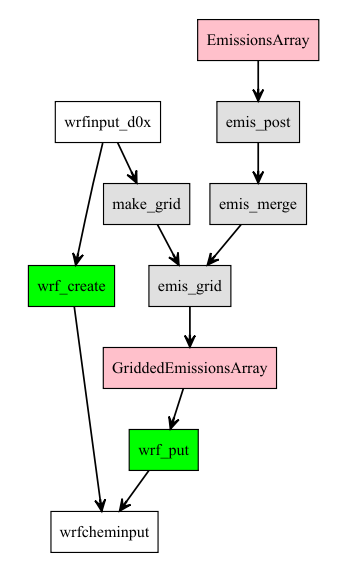
\includegraphics[width=0.5\linewidth]{figuras/gea} 

}

\caption{Generation of wrfchem inputs using GriddedEmissionsArray}\label{fig:gea}
\end{figure}

Example

\subsection{Creating a WRF-Chem input
file}\label{creating-a-wrf-chem-input-file}

The emission file will be generated with traffic simulation from the
Traffic Engineering Company (CET) for 2012, which consists in traffic
flow for morning rush hour of Light Duty Vehicles (LDV). The emission
factors will be the data \texttt{fe2015} and the wrfinput comes from the
\texttt{eixport} package. Let's go:

\subsubsection{0) Network}\label{network}

The object net has a class \texttt{SpatialLinesDataFrame}, we transform
it into a \texttt{sf}object. The length of the road is the field `lkm'
in the object net, which are in km but has no units. We must add the
right units in order to use \texttt{vein}

\begin{Shaded}
\begin{Highlighting}[]
\KeywordTok{require}\NormalTok{(vein)}
\KeywordTok{require}\NormalTok{(sf)}
\KeywordTok{require}\NormalTok{(units)}
\NormalTok{net <-}\StringTok{ }\KeywordTok{readRDS}\NormalTok{(}\StringTok{"figuras/net.rds"}\NormalTok{)}
\KeywordTok{class}\NormalTok{(net)}
\NormalTok{net <-}\StringTok{ }\NormalTok{sf}\OperatorTok{::}\KeywordTok{st_as_sf}\NormalTok{(net)}
\NormalTok{net[}\DecValTok{1}\NormalTok{, ]}
\NormalTok{net}\OperatorTok{$}\NormalTok{lkm <-}\StringTok{ }\NormalTok{units}\OperatorTok{::}\KeywordTok{set_units}\NormalTok{(}\KeywordTok{st_length}\NormalTok{(net), km) }\CommentTok{# ensure right units}
\end{Highlighting}
\end{Shaded}

\subsubsection{1) Vehicular composition}\label{vehicular-composition-1}

In this case, the vehicular composition consits in only to vehicles,
Passenger Cars using Gasoline with 25\% of Ethanol and Light Trucks
consuming Diesel with 5\% od biodiesel. Also, the emission factors cover
\(CO\). The temporal distribution will cover only one hour.

\begin{Shaded}
\begin{Highlighting}[]
\NormalTok{PC_E25 <-}\StringTok{ }\KeywordTok{age_ldv}\NormalTok{(net}\OperatorTok{$}\NormalTok{ldv)}
\end{Highlighting}
\end{Shaded}

\subsubsection{2) Emission factors}\label{emission-factors}

The emission factors used comes from \citet{CETESB2015}, which are
constant by age of use. In practice, this data.frame is like an Excel
spreadsheet. Then, the constructor function \texttt{EmissionFactorsList}
convert our numeric vector, which is the column of our data.frame, into
required type of object of the \texttt{emis} function. Parenthesis were
added in order to print the objects in one line.

\begin{Shaded}
\begin{Highlighting}[]
\KeywordTok{data}\NormalTok{(fe2015)}
\NormalTok{(EF_CO_PC_E25 <-}\StringTok{ }\KeywordTok{EmissionFactorsList}\NormalTok{(fe2015[fe2015}\OperatorTok{$}\NormalTok{Pollutant }\OperatorTok{==}\StringTok{ "CO"}\NormalTok{, }\StringTok{"PC_G"}\NormalTok{]))}
\end{Highlighting}
\end{Shaded}

\subsubsection{3) Estimation of
emissions}\label{estimation-of-emissions}

The estimation of emissions is shown in the following code chunk in a
simplified way. The emissions array are aggregated.

\begin{Shaded}
\begin{Highlighting}[]
\KeywordTok{data}\NormalTok{(profiles)}
\NormalTok{emi <-}\StringTok{ }\KeywordTok{emis}\NormalTok{(}\DataTypeTok{veh =}\NormalTok{ PC_E25, }\DataTypeTok{lkm =}\NormalTok{ net}\OperatorTok{$}\NormalTok{lkm, }\DataTypeTok{ef =}\NormalTok{ EF_CO_PC_E25,}
             \DataTypeTok{profile =}\NormalTok{ profiles}\OperatorTok{$}\NormalTok{PC_JUNE_}\DecValTok{2012}\NormalTok{)}
\end{Highlighting}
\end{Shaded}

\subsubsection{4) Post-estimations}\label{post-estimations}

The resulting emissions array \texttt{emi} is now processed with
\texttt{emis\_post}.

\begin{Shaded}
\begin{Highlighting}[]
\NormalTok{co_street <-}\StringTok{ }\KeywordTok{emis_post}\NormalTok{(}\DataTypeTok{arra =}\NormalTok{ emi, }\DataTypeTok{by =} \StringTok{"streets_wide"}\NormalTok{, }\DataTypeTok{net =}\NormalTok{ net)}
\end{Highlighting}
\end{Shaded}

\paragraph{\texorpdfstring{4a WRFChem input file with
\texttt{eixport}}{4a WRFChem input file with eixport}}\label{a-wrfchem-input-file-with-eixport}

Now it is time generate the emissions grid. In order to create a wrfchem
input file, we need a wrfinput file. In this case, the wrfinput coversa
wider area of the emissions, located in São Paulo, Brazil. The wrfinput
file is available from the R package \texttt{eixport}.

\begin{Shaded}
\begin{Highlighting}[]
\NormalTok{wrf <-}\StringTok{ }\KeywordTok{paste}\NormalTok{(}\KeywordTok{system.file}\NormalTok{(}\StringTok{"extdata"}\NormalTok{, }\DataTypeTok{package =} \StringTok{"eixport"}\NormalTok{),}
             \StringTok{"/wrfinput_d02"}\NormalTok{, }\DataTypeTok{sep=}\StringTok{""}\NormalTok{)}
\NormalTok{g  <-}\StringTok{ }\KeywordTok{make_grid}\NormalTok{(wrf)}
\end{Highlighting}
\end{Shaded}

\begin{verbatim}
## path to wrfinput
\end{verbatim}

\begin{verbatim}
## using grid info from: /home/sergio/R/x86_64-pc-linux-gnu-library/3.5/eixport/extdata/wrfinput_d02 
## Number of lat points 51
## Number of lon points 63
\end{verbatim}

\begin{Shaded}
\begin{Highlighting}[]
\KeywordTok{plot}\NormalTok{(}\KeywordTok{st_geometry}\NormalTok{(g), }\DataTypeTok{axes =} \OtherTok{TRUE}\NormalTok{)}
\KeywordTok{plot}\NormalTok{(}\KeywordTok{st_geometry}\NormalTok{(co_street), }\DataTypeTok{add =} \OtherTok{TRUE}\NormalTok{)}
\end{Highlighting}
\end{Shaded}

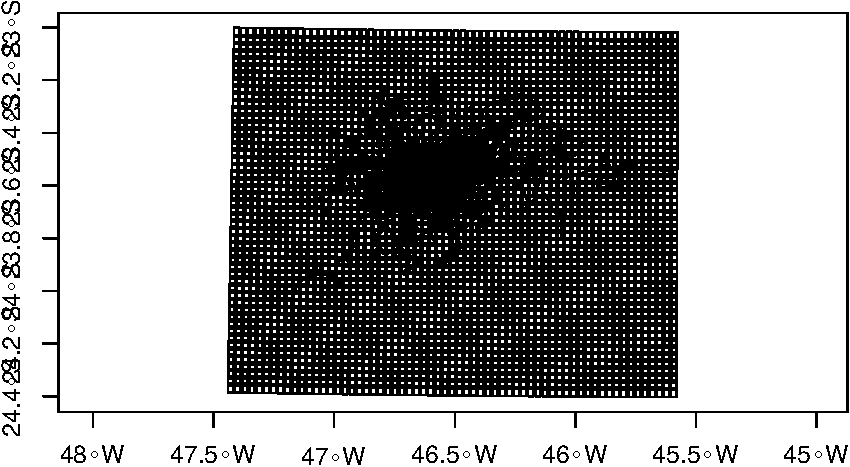
\includegraphics{veinbook_files/figure-latex/9.8-1.pdf}

Notice that weh we create grid from the path to wrfinput, there is a
message with \emph{Number of lat points 51} and \emph{Number of lon
points 63}. This information is crytical for later conversions. Now that
we have the street emissions and the grid, we can obtain our gridded
emissions:

\begin{Shaded}
\begin{Highlighting}[]
\NormalTok{gCO <-}\StringTok{ }\KeywordTok{emis_grid}\NormalTok{(}\DataTypeTok{spobj =}\NormalTok{ co_street, }\DataTypeTok{g =}\NormalTok{ g)}
\end{Highlighting}
\end{Shaded}

\begin{verbatim}
## Sum of street emissions 1845699895.43
\end{verbatim}

\begin{verbatim}
## although coordinates are longitude/latitude, st_intersection assumes that they are planar
\end{verbatim}

\begin{verbatim}
## Sum of gridded emissions 1845699895.43
\end{verbatim}

\begin{Shaded}
\begin{Highlighting}[]
\KeywordTok{names}\NormalTok{(gCO)}
\end{Highlighting}
\end{Shaded}

\begin{verbatim}
##   [1] "id"       "V1"       "V2"       "V3"       "V4"       "V5"      
##   [7] "V6"       "V7"       "V8"       "V9"       "V10"      "V11"     
##  [13] "V12"      "V13"      "V14"      "V15"      "V16"      "V17"     
##  [19] "V18"      "V19"      "V20"      "V21"      "V22"      "V23"     
##  [25] "V24"      "V25"      "V26"      "V27"      "V28"      "V29"     
##  [31] "V30"      "V31"      "V32"      "V33"      "V34"      "V35"     
##  [37] "V36"      "V37"      "V38"      "V39"      "V40"      "V41"     
##  [43] "V42"      "V43"      "V44"      "V45"      "V46"      "V47"     
##  [49] "V48"      "V49"      "V50"      "V51"      "V52"      "V53"     
##  [55] "V54"      "V55"      "V56"      "V57"      "V58"      "V59"     
##  [61] "V60"      "V61"      "V62"      "V63"      "V64"      "V65"     
##  [67] "V66"      "V67"      "V68"      "V69"      "V70"      "V71"     
##  [73] "V72"      "V73"      "V74"      "V75"      "V76"      "V77"     
##  [79] "V78"      "V79"      "V80"      "V81"      "V82"      "V83"     
##  [85] "V84"      "V85"      "V86"      "V87"      "V88"      "V89"     
##  [91] "V90"      "V91"      "V92"      "V93"      "V94"      "V95"     
##  [97] "V96"      "V97"      "V98"      "V99"      "V100"     "V101"    
## [103] "V102"     "V103"     "V104"     "V105"     "V106"     "V107"    
## [109] "V108"     "V109"     "V110"     "V111"     "V112"     "V113"    
## [115] "V114"     "V115"     "V116"     "V117"     "V118"     "V119"    
## [121] "V120"     "V121"     "V122"     "V123"     "V124"     "V125"    
## [127] "V126"     "V127"     "V128"     "V129"     "V130"     "V131"    
## [133] "V132"     "V133"     "V134"     "V135"     "V136"     "V137"    
## [139] "V138"     "V139"     "V140"     "V141"     "V142"     "V143"    
## [145] "V144"     "V145"     "V146"     "V147"     "V148"     "V149"    
## [151] "V150"     "V151"     "V152"     "V153"     "V154"     "V155"    
## [157] "V156"     "V157"     "V158"     "V159"     "V160"     "V161"    
## [163] "V162"     "V163"     "V164"     "V165"     "V166"     "V167"    
## [169] "V168"     "geometry"
\end{verbatim}

\begin{Shaded}
\begin{Highlighting}[]
\NormalTok{gCO}\OperatorTok{$}\NormalTok{geometry}
\end{Highlighting}
\end{Shaded}

\begin{verbatim}
## Geometry set for 3213 features 
## geometry type:  POLYGON
## dimension:      XY
## bbox:           xmin: -47.43966 ymin: -24.4031 xmax: -45.57575 ymax: -23.00105
## epsg (SRID):    4326
## proj4string:    +proj=longlat +datum=WGS84 +no_defs
## First 5 geometries:
\end{verbatim}

\begin{verbatim}
## POLYGON ((-47.41831 -24.35009, -47.41831 -24.38...
\end{verbatim}

\begin{verbatim}
## POLYGON ((-47.38871 -24.35053, -47.38871 -24.38...
\end{verbatim}

\begin{verbatim}
## POLYGON ((-47.35907 -24.35097, -47.35907 -24.38...
\end{verbatim}

\begin{verbatim}
## POLYGON ((-47.32947 -24.35143, -47.32947 -24.38...
\end{verbatim}

\begin{verbatim}
## POLYGON ((-47.29984 -24.35187, -47.29984 -24.38...
\end{verbatim}

This function requires the package \texttt{lwgeom} when the data is in
latitude and longitude degrees. There are some messages about the total
emissions of street and grid. This was made in order to ensure that
emis\_grid is conservative. The resulting object \texttt{gCO} is an
\texttt{sf} object of POLYGON. In order to plot the emissions, i
selected the emissions above 1, because it is easier to see the plot. If
we plot the gridded emissions, we will see:

\begin{Shaded}
\begin{Highlighting}[]
\NormalTok{gCO}\OperatorTok{$}\NormalTok{V9 <-}\StringTok{ }\NormalTok{gCO}\OperatorTok{$}\NormalTok{V9}\OperatorTok{*}\NormalTok{(}\DecValTok{12} \OperatorTok{+}\StringTok{ }\DecValTok{16}\NormalTok{)}\OperatorTok{^-}\DecValTok{1}
\KeywordTok{plot}\NormalTok{(gCO[gCO}\OperatorTok{$}\NormalTok{V9 }\OperatorTok{>}\DecValTok{1}\NormalTok{, }\StringTok{"V9"}\NormalTok{], }\DataTypeTok{axes =} \OtherTok{TRUE}\NormalTok{,  }\DataTypeTok{nbreaks =} \DecValTok{50}\NormalTok{,}
     \DataTypeTok{pal =}\NormalTok{ cptcity}\OperatorTok{::}\KeywordTok{cpt}\NormalTok{(}\DataTypeTok{colorRampPalette =}\NormalTok{ T),}
     \DataTypeTok{main =} \StringTok{"Emissions of CO at 08:00 (mol/h)"}\NormalTok{)}
\end{Highlighting}
\end{Shaded}

\begin{figure}
\centering
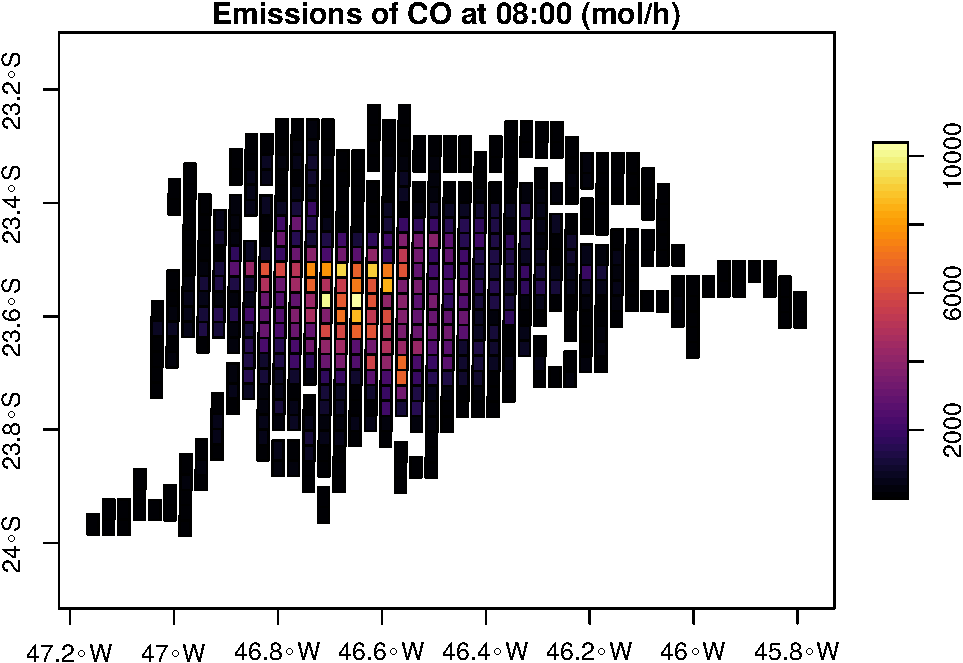
\includegraphics{veinbook_files/figure-latex/GEmi-1.pdf}
\caption{\label{fig:GEmi}Gridded emissions (mol/h)}
\end{figure}

The emissions are mostly distributed into main roads, as expected. The
next step is create the \texttt{GriddedEmissionsArray} that will be
inputted into the \texttt{eixport} functions. The
\texttt{GriddedEmissionsArray} is a contructor function that reads
class, \texttt{SpatialPolygonDataFrame}, \texttt{sf} of POLYGONs, a
\texttt{data.frame} or a \texttt{matrix} to create an Array of the
gridded emissions. The dimensions are lat, lon, mass and time.
Therefore, it is important to know the number of lat and lon points!

\begin{Shaded}
\begin{Highlighting}[]
\NormalTok{gCOA <-}\StringTok{ }\KeywordTok{GriddedEmissionsArray}\NormalTok{(}\DataTypeTok{x =}\NormalTok{ gCO, }\DataTypeTok{cols =} \DecValTok{63}\NormalTok{, }\DataTypeTok{rows =} \DecValTok{51}\NormalTok{, }\DataTypeTok{times =} \DecValTok{168}\NormalTok{)}
\end{Highlighting}
\end{Shaded}

\begin{verbatim}
## This GriddedEmissionsArray has:
##  51 lat points
##  63 lon points
##  168 hours
\end{verbatim}

\begin{Shaded}
\begin{Highlighting}[]
\KeywordTok{plot}\NormalTok{(gCOA, }\DataTypeTok{col =}\NormalTok{ cptcity}\OperatorTok{::}\KeywordTok{cpt}\NormalTok{())}
\end{Highlighting}
\end{Shaded}

\begin{figure}
\centering
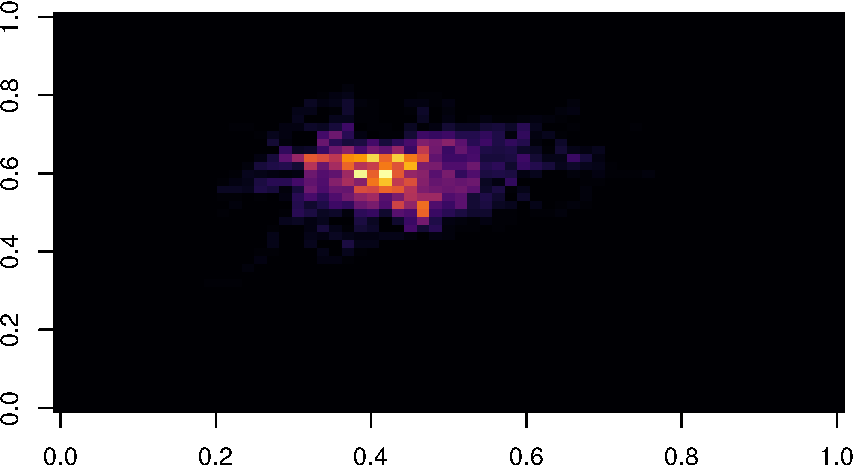
\includegraphics{veinbook_files/figure-latex/GEA-1.pdf}
\caption{\label{fig:GEA}GriddedEmissionsArray (mol/h)}
\end{figure}

The image is similar to the plot of the gridded emissions, which means
that it is correct. Now we can input the our new created object
\texttt{gCOA} into the wrfchem input file, but first, we need to create
it. This is done using the \texttt{eixport} functions.

We first load the library \texttt{eixport}. Then load the data
\texttt{emis\_opt} which has the emissions options for WRFchem. In this
case, we are creating an wrfchem input file with 40 pollutants, with 0.

\begin{Shaded}
\begin{Highlighting}[]
\KeywordTok{library}\NormalTok{(eixport)}
\KeywordTok{data}\NormalTok{(emis_opt)}
\NormalTok{emis_opt[[}\StringTok{"ecb05_opt1"}\NormalTok{]]}
\KeywordTok{wrf_create}\NormalTok{(}\DataTypeTok{wrfinput_dir =} \KeywordTok{system.file}\NormalTok{(}\StringTok{"extdata"}\NormalTok{, }\DataTypeTok{package =} \StringTok{"eixport"}\NormalTok{),}
           \DataTypeTok{wrfchemi_dir =} \KeywordTok{tempdir}\NormalTok{(),}
           \DataTypeTok{frames_per_auxinput5 =} \DecValTok{168}\NormalTok{,}
           \DataTypeTok{domains =} \DecValTok{2}\NormalTok{,}
           \DataTypeTok{variaveis =}\NormalTok{ emis_opt[[}\StringTok{"ecb05_opt1"}\NormalTok{]],}
           \DataTypeTok{verbose =}\NormalTok{ F)}
\end{Highlighting}
\end{Shaded}

The wrfchemi input file was created on a temporal directory with the
function \texttt{tempdir}. Now we can input our
\texttt{GriddedEmissionsArray} into our new wrfchem input file.

\begin{Shaded}
\begin{Highlighting}[]
\NormalTok{f <-}\StringTok{ }\KeywordTok{list.files}\NormalTok{(}\DataTypeTok{path =} \KeywordTok{tempdir}\NormalTok{(), }\DataTypeTok{full.names =}\NormalTok{ T, }\DataTypeTok{pattern =} \StringTok{"wrfchemi_d02"}\NormalTok{)}
\NormalTok{f}
\KeywordTok{wrf_put}\NormalTok{(}\DataTypeTok{file =}\NormalTok{ f, }\DataTypeTok{name =} \StringTok{"E_CO"}\NormalTok{, }\DataTypeTok{POL =}\NormalTok{ gCOA)}
\end{Highlighting}
\end{Shaded}

Then, we just check our resulting NetCDF file plotting the emissions we
just put.

\begin{Shaded}
\begin{Highlighting}[]
\KeywordTok{wrf_plot}\NormalTok{(f, }\StringTok{"E_CO"}\NormalTok{)}
\end{Highlighting}
\end{Shaded}

\begin{figure}

{\centering 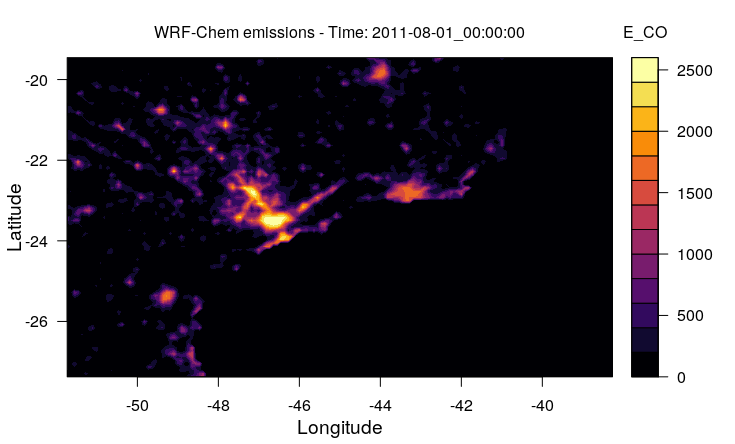
\includegraphics[width=0.8\linewidth]{figuras/wrf2} 

}

\caption{Wrfchem input file (NetCDF) (mol/h)}\label{fig:wrf}
\end{figure}

\paragraph{\texorpdfstring{4b WRFChem input file with
\texttt{emis\_wrf}}{4b WRFChem input file with emis\_wrf}}\label{b-wrfchem-input-file-with-emis_wrf}

\texttt{emis\_wrf} creates a \texttt{data.frame} with columns lat, long,
id, pollutants, local time and GMT time. This dataframe has the proper
format to be used with WRF assimilation system: ``ASimilation System 4
WRF (AS4WRF, \citet{angel})

\begin{Shaded}
\begin{Highlighting}[]
\KeywordTok{args}\NormalTok{(emis_wrf)}
\end{Highlighting}
\end{Shaded}

\begin{verbatim}
## function (sdf, nr = 1, dmyhm, tz, crs = 4326, islist, utc) 
## NULL
\end{verbatim}

where:

\begin{itemize}
\tightlist
\item
  \texttt{sdf}: Gridded emissions, which can be a
  SpatialPolygonsDataFrame, or a list of SpatialPolygonsDataFrame, or a
  sf object of ``POLYGON''. The user must enter a list with 36
  SpatialPolygonsDataFrame with emissions for the mechanism CBM-Z.
\item
  \texttt{nr}: Number of repetitions of the emissions period
\item
  \texttt{dmyhm}: String indicating Day Month Year Hour and Minute in
  the format ``d-m-Y H:M'' e.g.: ``01-05-2014 00:00'' It represents the
  time of the first hour of emissions in Local Time
\item
  \texttt{tz}: Time zone as required in for function as.POSIXct
\item
  \texttt{crs}: Coordinate reference system, e.g: ``+init=epsg:4326''.
  Used to transform the coordinates of the output
\item
  \texttt{islist}: logical value to indicate if sdf is a list or not
\item
  \texttt{utc}: ignored.
\end{itemize}

In this case, we can use our gridded emissions directly here:

\begin{Shaded}
\begin{Highlighting}[]
\NormalTok{gCO}\OperatorTok{$}\NormalTok{id <-}\StringTok{ }\OtherTok{NULL}
\NormalTok{df <-}\StringTok{ }\KeywordTok{emis_wrf}\NormalTok{(}\DataTypeTok{sdf =}\NormalTok{ gCO, }\DataTypeTok{dmyhm =} \StringTok{"06-10-2014 00:00"}\NormalTok{,}
               \DataTypeTok{tz =} \StringTok{"America/Sao_Paulo"}\NormalTok{, }\DataTypeTok{islist =} \OtherTok{FALSE}\NormalTok{)}
\end{Highlighting}
\end{Shaded}

\begin{verbatim}
## You can create wrchem inputs directly with 
## eixport::create and eixport::wrf_put
## https://CRAN.R-project.org/package=eixport
\end{verbatim}

\begin{Shaded}
\begin{Highlighting}[]
\KeywordTok{head}\NormalTok{(df)}
\end{Highlighting}
\end{Shaded}

\begin{verbatim}
##    id      long       lat pollutant    time_lt            time_utc dutch
## 1   1 -47.41831 -24.35009         0 2014-10-06 2014-10-06 03:00:00   600
## 6   2 -47.38871 -24.35053         0 2014-10-06 2014-10-06 03:00:00   600
## 11  3 -47.35907 -24.35097         0 2014-10-06 2014-10-06 03:00:00   600
## 16  4 -47.32947 -24.35143         0 2014-10-06 2014-10-06 03:00:00   600
## 21  5 -47.29984 -24.35187         0 2014-10-06 2014-10-06 03:00:00   600
## 26  6 -47.27024 -24.35230         0 2014-10-06 2014-10-06 03:00:00   600
\end{verbatim}

Then you must export this \texttt{data.frame} into a .txt file. You must
include the number of columns to match your luped species and also take
out the columns time\_lt, time\_utc and dutch. These three columns are
just informative.

\begin{Shaded}
\begin{Highlighting}[]
\NormalTok{df <-}\StringTok{ }\NormalTok{df[,}\DecValTok{1}\OperatorTok{:}\DecValTok{4}\NormalTok{]}
\KeywordTok{write.table}\NormalTok{(}\DataTypeTok{x =}\NormalTok{ df, }\DataTypeTok{file =} \KeywordTok{tempfile}\NormalTok{(), }\DataTypeTok{sep =} \StringTok{"}\CharTok{\textbackslash{}t}\StringTok{"}\NormalTok{,}
            \DataTypeTok{col.names =} \OtherTok{TRUE}\NormalTok{, }\DataTypeTok{row.names =} \OtherTok{FALSE}\NormalTok{)}
\end{Highlighting}
\end{Shaded}

Finally, in order to generate the wrfchem input file, you must have the
resulting .txt file, a wrfinput file with the same grid spacing, the NCL
script AS4WRF and a namelist. AS4WRF and the namelist can be obtained
contacting
\href{mailto:angel.vela@iag.usp.br}{\nolinkurl{angel.vela@iag.usp.br}}
and \href{mailto:alvv1986@gmail.com}{\nolinkurl{alvv1986@gmail.com}}.

\chapter{Quality check and errors}\label{check}

This last chapter of this book presents to aspestcs fthat must be
considered for any practicioner interested in developing emissions
inventories. The first part covers a summary of the EMEP/EEA air
pollutant emission inventory guidebook 2016, Technical guidance to
prepare national emission inventories \citep{guia}, based on the
Intergovernmental Panel on Climate Change (IPCC) 2006 Good Practice
Guidance {[}\citet{change20062006}. The second part consists in advices
and specific considerations for avoinding errors when runnign VEIN in
each part of the inventory.

\section{Guidance from EMEP/EEA air pollutant emission inventory
guidebook}\label{guidance-from-emepeea-air-pollutant-emission-inventory-guidebook}

I believe that this part of this capter delivers knowledge that you
really will gain with experience. But even with experience you can get
lost, and returning to this part would save you. This part is based on
the EMEP/EEA air pollutant emission inventory guidebook \citep{guia}.

\subsection{Key categories}\label{key-categories}

Key categories are the most important \textbf{source} categories. This
section is based on the chapter Key category analysis and methodological
choice \citep{guiak} of the EMEP/EEA air pollutant emission inventory
guidebook 2013. They are important because they are responsabile for
most of pollution in a determined region. For instance, it has been
described that vehicles are the most important source of pollution in
mega-cities \citep{molina2004megacities}. Evenmore, in the case of São
Paulo, the official emissions inventory informs that vehicles are
responsabiel for mor than 97 \% of \(CO\), 79 \% of \(HC\), 68 \% of
\(NO_X\), and only 29 \% of \(PM\) and 22 \% of \(SO_X\)
\citep{CETESB2015}. This shown another characteristics of key
categories: they depend of specific pollutants.

For another example, consider a city which suffers cold weather with use
bio-mass burning for cooking and heating. The main source of
\(PM_{2.5}\) will be certainly bio-mass burning.

Now consider an industrial region with industrial process that emit too
much \(SO_X\). The key-cateogries might be industrial sources.

And one more example, consider a huge mega-city with electric mobility.
However, the main source of electricity are thermoelectric based on
carbon (the key).

This implies that it should be a nomemclature for categorizing and
naming sources. IPCC, has a nomenclature for instance.

The ideia behind key categories, is that most efforts must be applied in
this categories, obtainging the highest level of detail with less
uncertainty. Hence, the emissions guidelines \citep{guia} proposes three
levels of complexity estimation methods, known as Tier Methods. The
complexity increases from level 1, 2 and 3. The VEIN tier is 3, which is
that the most complex function of vehicular emissions estimations are
incporated, with the exception of evaporative. I need to improve that
part.

\begin{itemize}
\tightlist
\item
  Tier 1: a simpler method which include available activity and
  emissions factors.
\item
  Tier 2: Similar to Tier 1, but includes more specific emission
  factors.
\item
  Tier 3: Most complex methodologies with higher level of detail,
  temporal and spatial.
\end{itemize}

\subsection{Uncertainty}\label{uncertainty}

This is a very important part in any emissions inventory and a dedicated
chapter or section should be made in any report/paper. This section is
based on the chapter Uncertainties \citep{guiau} of the EMEP/EEA air
pollutant emission inventory guidebook 2013.The 2006 IPCC Guidelines
chapter states that estimating the uncertainty of an inventory is needed
\citep{change20062006}.

It is recommended to use 95\% confidence interval. This means that:

\begin{itemize}
\tightlist
\item
  there is a 95\% of probability that the actual value of the quantity
  estimates is within the interval defined by the confidence interval.
\item
  The probability of the actual value will be outside the range it is
  5\%.
\end{itemize}

The general form for estimating emissions was shown on Eq.
\eqref{eq:efGERAL} \citep{guiau}. This equation will be the base for
calculating the uncertainty. This section is applied when measurements
are made, for the case of activity or emission factors. In those case,
it is possible calculate the required confiden intervals.

\subsubsection{Default uncertainty
ranges}\label{default-uncertainty-ranges}

\emph{Activity data}

The following table is taking directly form \citet{guia} and propose
indicative ranges that could be applies in cases where no independed
data are available.

\begin{itemize}
\tightlist
\item
  National official statistics: - .
\item
  Update of last year's statistics using Gross Economic Growth factors:
  0 - 2\%.
\item
  International Energy Agency (IEA) statistics: OECD: 2 - 3\%, non-OECD
  5-10\%.
\item
  United Nation data bases: 5 - 10\%.
\item
  Default values, other sources: 30 - 100\%.
\end{itemize}

\emph{Emission factors}

The following table is taking directly form \citet{guia} and propose
rating definitions for emission factors\citep{guia}.

\begin{itemize}
\tightlist
\item
  A: An estimate based on a large number of measurements made at a large
  number of facilities that fully represent the sector. Error: 10 o
  30\%.
\item
  B: An estimate based on a large number of measurements made at a large
  number of facilities that represent a large part of the sector. Error:
  20 to 60\%
\item
  C: An estimate based on a number of measurements made at a small
  number of representative facilities, or an engineering judgement based
  on a number of relevant facts. Error: 50 to 200\%.
\item
  D: An estimate based on single measurements, or an engineering
  calculation derived from a number of relevant facts. Error: 100 to
  300\%.
\item
  E: An estimate based on an engineering calculation derived from
  assumptions only. Error: Order of magnitude.
\end{itemize}

In \citet{guia} appears ratings for road transport emission factors that
diffier from the ratings that appear in
\citet{NtziachristosSamaras2016}. To preserve consistenty in this book,
here is presented the precision indicators, Table 4-1 of
\citet{NtziachristosSamaras2016} report.

\begin{table}

\caption{\label{tab:precision}Precision indicators (Ntziachristos and Samaras 2016)}
\centering
\begin{tabular}[t]{l|l|l|l|l|l|l|l|l}
\hline
Category & NOx & CO & NMHC & CH4 & PM & N2O & NH3 & CO2\\
\hline
PC G w/o Catalyst & A & A & A & A & - & C & C & A\\
\hline
PC G w Catalyst & A & A & A & A & - & A & A & A\\
\hline
PC D & A & A & A & A & A & B & B & A\\
\hline
PC LPG & A & A & A & - & - & - & - & A\\
\hline
PC LPG w/o Catalyst & A & A & A & A & D & C & C & A\\
\hline
PC LPG w Catalyst & D & D & D & D & D & D & D & A\\
\hline
PC 2 strokes & B & B & B & D & - & D & D & B\\
\hline
LCV G & B & B & B & C & - & B & B & A\\
\hline
LCV D & B & B & B & C & A & B & B & A\\
\hline
HDV G & D & D & D & C & - & D & D & D\\
\hline
HDV D & A & A & A & D & A & B & B & A\\
\hline
MC cc <50 & A & A & A & B & - & B & B & A\\
\hline
MC cc > 50 2 strokes & A & A & A & B & - & B & B & A\\
\hline
MC cc > 50 4 strokes & A & A & A & B & - & B & B & A\\
\hline
Cold-start PC G Pre Euro & B & B & B & - & - & - & - & B\\
\hline
Cold-start PC G Euros & B & B & B & A & - & - & - & A\\
\hline
Cold-start PC D Pre Euro & C & C & C & - & C & - & - & B\\
\hline
Cold-start PC D Euros & A & A & A & A & A & - & - & A\\
\hline
Cold-start PC LPG & C & C & C & - & - & - & - & B\\
\hline
Cold-start LCV G & D & D & D & - & - & - & - & D\\
\hline
Cold-start LCV F & D & D & D & - & D & - & - & D\\
\hline
\end{tabular}
\end{table}

Uncertainties can be aggregated with two approaches

\begin{itemize}
\tightlist
\item
  \emph{Rule A}: uncertainties are combined by \emph{addition}, as shown
  in Eq. \eqref{eq:sumun}:
\end{itemize}

\begin{equation}
U_{total}=\frac{\sqrt{\sum_{i = 1}^{n}(U_i \cdot x_i )^2}}{\sum_{i = 1}^{n}}
\label{eq:sumun}
\end{equation}

Where, \(x\) are the quantities, \(U_i\) are the uncertain quantities
and the percentage uncertainties (half the 95\% confidence interval)
associated with them, respectivly. \(U_{total}\) is the percentage
uncertinti in the sum of the quantites (half the 95\% confidence
interval divided by the total (i.e.~mean) and expressed as percentage).

\begin{itemize}
\tightlist
\item
  \emph{Rule B}: uncertainties are combined by \emph{multiplication}, as
  shown on Eq. \eqref{eq:sumul}:
\end{itemize}

\begin{equation}
U_{total}=\sqrt{\sum_{i = 1}^{n}(U_i)^2} 
\label{eq:sumul}
\end{equation}

Where, \(U_i\) are the percentage quantities (hal the 95\% confidence
interval) associated with each of the quantities. \(U_{total}\) is the
percentage in the product of the quantities (half the 95\% confidence
interval divided by the total and expressed as percentage).

Alternatively, a Monte Carlo simulation can be done.

\subsection{Quality Assurance and Quality
Check}\label{quality-assurance-and-quality-check}

This section is mostly based on the chapter Inventory management,
improvement and QA/QC \citep{guiaqa} of the EMEP/EEA air pollutant
emission inventory guidebook 2013.

According to Wikipedia:

\begin{itemize}
\tightlist
\item
  \textbf{Quality assurance (QA)} is a way of preventing mistakes and
  defects in manufactured products and avoiding problems when delivering
  solutions or services to customers \citep{wiki:qa}.
\item
  \textbf{Quality control (QC)} is a process by which entities review
  the quality of all factors involved in production \citep{wiki:qc}.
\end{itemize}

The main reference in QA/QC are the International Organization for
Standardization ISO 9000 \citep{wiki:iso}.

The idea is to avoid errors in the development of the inventory. Hence,
it is very important that the objective of the inventory, frequency and
spatial and temporal resolution must be very clear. As mentioned before,
the inventory can have a purpose of policy application or scientific. In
any case, the QAQC procedures should be explicitly stated covering five
data quality objectives \textbf{transparency}, \textbf{consistency},
\textbf{comparability}, \textbf{completeness} and \textbf{acccuracy}.

This means that another researcher/practicioner should be able to
reproduce the results. However, this is not always the case. Evenmore,
it has been shown that there are currently a crisis of reproducibility
in science, where `more than 70\% of researchers have tried and failed
to reproduce another scientist's experiments, and more than half have
failed to reproduce their own experiments' \citep{baker2016there}. I
believe that emissions inventories should guarantee the reproducibility
of results, in scientific and policy application inventories.

\subsection{Inventory managment cycle}\label{inventory-managment-cycle}

Another important aspect is the inventory managment cycle. The inventory
manager is responsabile for institutional arrangments, meet deadlines
and for the inventory managment cycle. The inventory complier gets the
data and estimate the emissions with the respective Tier.

The cycle is:

\begin{enumerate}
\def\labelenumi{\arabic{enumi}.}
\tightlist
\item
  Priorization of improvements: As the resources are limited,
  priorization must be given to key categories.
\item
  Data-collection: It is important to stablish formal agreements needs
  with data providers using protocols. The protocols must cleary show
  the data needed, its format, content and dates of delivery.
\item
  Inventory compilation. The inventory compiler estimate the emissions.
\item
  Consolidation. The inventory manager consolidates all the emissions
  ensuring quality in data and methods for estimating emissions.
\item
  Data Quality Review.
\item
  Reporting.
\item
  Lessons learned and improvement review.
\item
  Inventory Managment Report.
\item
  Quality Assurance and Quality Control Plan.
\end{enumerate}

\section{Avoiding errors with VEIN}\label{avoiding-errors-with-vein}

The first part of this chapter covered some fundamental aspects in
emissions inventory managment for quality assurance and quality control.
This part covers typical erros that I've faced using VEIN and I hope it
help users how to avoid them.

Currently, VEIN does not have grafical user interface (GUI) and runs on
R \citep{R}, which can be intimidating for new users. Also, even
experienced users can do mistakes. If you find a mistake, write it down
to abooid it in future. Be organized. I recommend to code your inventory
keeping in mind that you will have to check your scripts in the future,
so it would be nice if in the first try your code looks nice. And also,
don't panic.

\subsection{Traffic flow}\label{traffic-flow}

One of the first inputs of it is the traffic flow data. You must have an
agreement with data providers to get the data. Also, the compiler must
understand the format of the data. In my experience, data providers
comes from government agencies with limitated resources and few time.
This means that, if there is not a formal agreement, they won't speed
too much time for processing their data to meet your needs (because it
is not part of their jobs). And even, if there was a formal agreement,
the data processing must be done by the data compiler.

The data provided in this book covers a travel demand output for
Metropolitan Are ofSão Paulo (MASP) made by the Traffic Company
Engineering of São Paulo, for the year 2012. The has the same content
inside VEIN package, with the exception that covers the whole MASP. The
data originally is in format MAPINFO. Therefore, the package \textbf{sf}
must be used to read the data.

\begin{Shaded}
\begin{Highlighting}[]
\KeywordTok{library}\NormalTok{(sf)}
\NormalTok{net <-}\StringTok{ }\KeywordTok{st_read}\NormalTok{(}\StringTok{"data/masp.TAB"}\NormalTok{)}
\end{Highlighting}
\end{Shaded}

The section @ref(\#traffic) shows details about this data.

\begin{itemize}
\tightlist
\item
  Have a meeting with data delivers to check and solve any doubt
  regarding the data.
\item
  Check if your data is projected or not. The data probably will be
  projected with a UTM zone, for instance code 31983
  \url{http://spatialreference.org/ref/epsg/sirgas-2000-utm-zone-23s/}.
  VEIN imports functions from \texttt{sf} and \texttt{lwgeom} which
  depend on GEOS libraries. This means that VEIN can work with data
  projected or not. Nevertheless, I suggest to work with projected data
  for your location.
\item
  Ensure that the data is correctly read and that there are no objects
  of class \texttt{factor} in the columns.
\item
  Make sure that of what are the units of the traffic flow and remember
  that most of VEIN functions are designed to work with hourly traffic
  flow.
\item
  Plot the data. Check if the data looks fine or have some mistakes.
\item
  Calculate the length of each road. Make proper transformations and
  \textbf{make sure} \textbf{that resulting length of road as
  \texttt{units} km}. I suggest to use the name lkm. This can be easily
  done with in R with packages \texttt{sf} and \texttt{units} installed.
  Let's say that your data is named \emph{net} and your data is already
  projected. Also, that your traffic flow is named \emph{ldv} for light
  duty vehicles and \emph{hdv} for heavy duty vehicles.
\end{itemize}

\begin{Shaded}
\begin{Highlighting}[]
\KeywordTok{plot}\NormalTok{(net[}\StringTok{"ldv"}\NormalTok{], }\DataTypeTok{axes =}\NormalTok{ T)}
\KeywordTok{plot}\NormalTok{(net[}\StringTok{"hdv"}\NormalTok{], }\DataTypeTok{axes =}\NormalTok{ T)}
\NormalTok{net}\OperatorTok{$}\NormalTok{lkm <-}\StringTok{ }\NormalTok{sf}\OperatorTok{::}\KeywordTok{st_length}\NormalTok{(net) }\CommentTok{#returns distance in meters}
\NormalTok{net}\OperatorTok{$}\ErrorTok{$}\NormalTok{lkm <-}\StringTok{ }\NormalTok{units}\OperatorTok{::}\KeywordTok{set_units}\NormalTok{(net}\OperatorTok{$}\NormalTok{lkm, km) }\CommentTok{#transform meters in km}
\end{Highlighting}
\end{Shaded}

Despite that this transformation can be done by dividing lkm by 1000,
this would be wrong because the \texttt{units} wouldn't change and they
must be \texttt{km}. Hence, using the functions of the \texttt{units}
package is the recommended way.

\subsection{Vehicular composition}\label{vehicular-composition-2}

The vehicular composition is a critical part in the emissions
inventories for vehicles. It consists in the percentage of each type of
vehicle and technology. Despite that it seems pretty straightforward,
making a mistake in this part of the emissions inventories would cost
lots of time. \textbf{Developing an} \textbf{emissions inventory is a
complex task, you must take great care in simple} \textbf{calculations,
because if the resutls are not consistent, it can take LOTS} \textbf{of
time, to find the error, usually when the dealines are dead}.

The function \texttt{inventory} needs the vehicular composition to
create the respective directories to run VEIN. I have the feeling that
most of model users like structured models with clear input and outputs.
VEIN is not like that, and this is in part due to the nature of the
emissions inventories. I could design a model that works perfectly with
one type of input, but in real life, a desired input is not always easy
to get. For instance, the traffic simulation used inside the model is
not easy to get, even in cities of developed countries. Hence, the
inventory compiler must struggle to do their job. Therefore, VEIN was
designed with flexibility and verstility on mind.

Anyways, the vehicular composition are the number of each type the
following vehicles: PC, LCV, HGB, BUS, MC. Then, each sub category will
be divided by type of age of use. For instance, the vehicular emissions
inventory for São Paulo State considers 4 type of vehicles:

\begin{itemize}
\tightlist
\item
  Particulate Cars using gasohol (Gasoline with 25\% of ethanol,
  PC\_25).
\item
  Particulate Cars Flex using gasohol (Gasoline with 25\% of ethanol,
  PC\_F25).
\item
  Particulate Cars Flex using ethanol (Gasoline with 25\% of ethanol,
  PC\_FE100).
\item
  Particulate Cars using ethanol (Gasoline with 25\% of ethanol,
  PC\_E100).
\end{itemize}

This means that the number of PC is 4.

Then each of this vehicles is divided by age of use. As consecuence, we
must know when each of these vehicle entered and went out of the market.
Again, for São Paulo conditions, Flex engines entered into market in
2003 and nowadays must of new cars are flex. Vehicles with engines
designed for burning ethanol had a peak in early 80s, but they went of
the market in 2006. Gasoline vehicles have been in circulation from the
beginning and CETESB inventory considers a life span of 40 years of use.

The same analyses must be done with each of the vehicle categories.

The distribution by age of use indirectly shows the technology
associated with emission standards by age of use.

\subsection{Units}\label{units}

Currently, VEIN checks that the variable lkm (length) must be in km.
This is to avoid that the user wrongly enter length in meters or without
units. As a result, the emissions woult be huge and wrong.

In the case of vehicles, currently there are not designed a unit of
``vehicles'' in VEIN. In transportation studies, it is used the unit
``equivalent vehicle'' which standarize each type of vehicle by its
size. For instance, LCV are sometimes equivalent of 1.2 vehicles. Buses
or HGV can be equuvalent to 2 or more vehicles. however, there are no
such typeof this things in VEIN and units managment is designed to
control emission factors and length.

The temporal dimension is also an aspect difficult to handle regarding
the units. This is because, sometimes mileage are correctly in km, but
the timespan is in one year. Threfore, the units magament is degined to
avoid errors with emission factors and calculation of emissions. This
means that a future version of VEIN will erradicate all temporal
dimensions ensure right calculation of mass only. This means that VEIN
will not chech if the data is hourly or anunual.

\subsection{Emission factors}\label{emission-factors-1}

When I started this book, VEIN contained few emission factors. Now, the
version 0.5.7 has all the 2016 emission factors of CETESB, almost 100
emisision factors from the European Emission guidelines the all the BASE
emission factors from the International Vehicle Model (IVE). The
functions to access this data are:

\begin{itemize}
\tightlist
\item
  ef\_cetesb.
\item
  ef\_ldv\_speed.
\item
  ef\_hdv\_speed.
\item
  ef\_ive.
\end{itemize}

I will be working to import emission factors from HBEFA model which are
based traffic situation (very cool).

\subsection{Deterioration}\label{deterioration}

VEIN currently cover the deterioration emission factors from the
Euroepan emission guidelines. This values results in a simply numeric
vector depending on standard, mileage, type of vehicle and pollutant.
However, it would be possible to use any other deterioation factors.

Ensure to use correctly the data and cite respective literature.

\subsection{Fuel evaluation}\label{fuel-evaluation}

It is a good practice to ensure that the mass of fuel consumed of
vehicle in your study area, matchs the fuel sale son your area. If not,
calibrate your emissions by number of vehicles (if bottom-up) or a
combination of vehicles and mileage (if top-down) to match fuel sales.

\subsection{Emissions estimation}\label{emissions-estimation}

Most of emission functions returns an array of emissions, which means a
matrix of matrices. The idea was that each dimension has a meaning but
I've been thinking that it is not necessary and each dimension should
have different nature, for instance, it is not necessary two dimensions
for time, despite that one indicates hour and the other days. So I mght
change that in future. Dont panic, I'm always trying to change the
functions without breaking older code.

I hope you liked this book.

\appendix \addcontentsline{toc}{chapter}{\appendixname}


\chapter*{Appendix A: Fast Example of
VEIN}\label{appendix-a-fast-example-of-vein}


\begin{Shaded}
\begin{Highlighting}[]
\KeywordTok{library}\NormalTok{(vein)}
\KeywordTok{inventory}\NormalTok{(}\DataTypeTok{name =} \KeywordTok{file.path}\NormalTok{(}\KeywordTok{tempdir}\NormalTok{(), }\StringTok{"YourCity"}\NormalTok{),}
          \DataTypeTok{show.dir =} \OtherTok{TRUE}\NormalTok{,}
          \DataTypeTok{show.scripts =} \OtherTok{TRUE}\NormalTok{)}
\KeywordTok{source}\NormalTok{(}\KeywordTok{paste0}\NormalTok{(}\KeywordTok{file.path}\NormalTok{(}\KeywordTok{tempdir}\NormalTok{(), }\StringTok{"YourCity"}\NormalTok{), }\StringTok{"main.R"}\NormalTok{))}
\end{Highlighting}
\end{Shaded}

\chapter*{Appendix B: Detailed Example of
VEIN}\label{appendix-b-detailed-example-of-vein}


\section{Network}\label{network-1}

\begin{Shaded}
\begin{Highlighting}[]
\KeywordTok{inventory}\NormalTok{(}\KeywordTok{file.path}\NormalTok{(}\KeywordTok{tempdir}\NormalTok{(), }\StringTok{"YourCity"}\NormalTok{))}
\KeywordTok{setwd}\NormalTok{(}\StringTok{"YourCity"}\NormalTok{)}
\KeywordTok{data}\NormalTok{(net) }\CommentTok{# Loads the traffic demand simulation for west São Paulo}
\KeywordTok{data}\NormalTok{(net)}
\KeywordTok{data}\NormalTok{(pc_profile)}
\NormalTok{pc_week <-}\StringTok{ }\KeywordTok{temp_fact}\NormalTok{(net}\OperatorTok{$}\NormalTok{ldv}\OperatorTok{+}\NormalTok{net}\OperatorTok{$}\NormalTok{hdv, pc_profile)}
\NormalTok{speed <-}\StringTok{ }\KeywordTok{netspeed}\NormalTok{(pc_week, net}\OperatorTok{$}\NormalTok{ps, net}\OperatorTok{$}\NormalTok{ffs, net}\OperatorTok{$}\NormalTok{capacity, net}\OperatorTok{$}\NormalTok{lkm)}
\KeywordTok{saveRDS}\NormalTok{(net, }\DataTypeTok{file =} \StringTok{"network/net.rds"}\NormalTok{)}
\KeywordTok{saveRDS}\NormalTok{(speed, }\DataTypeTok{file =} \StringTok{"network/speed.rds"}\NormalTok{)}
\end{Highlighting}
\end{Shaded}

\section{\texorpdfstring{Vehicular composition
\citep{CETESB2015}}{Vehicular composition {[}@CETESB2015{]}}}\label{vehicular-composition-cetesb2015}

The vehicular composition \texttt{vehcomp} has 5 types of vehicles:
Passenger Carss (PC), Light Commercial Vehicles (LCV), Heavy Good
Vehicles or trucks (HGV), Buses (BUS), and Motorcycles (MC). The default
value of this argument is:
\texttt{c(PC\ =\ 4,\ LCV\ =\ 5,\ HGV\ =\ 5,\ BUS\ =\ 3,\ MC\ =\ 9)},
which means that there are 4 types of PC, 5 of LCV, 5 of trucks, 3 of
buses and 9 types of motorcycles. This composition comes from the
vehicular emissions inventory of the Environmental Agency of São Paulo,
Brazil \citep{CETESB2015}. In Brazil, the fuel used in vehicles is
blended with ethanol with and biodiesel. The user can use \textbf{any}
vehicular composition that representes its fleet with up-to 99 type of
vehicles per category. The default composition according Brazilian
emissions inventory is:

\emph{Passenger Cars (PC)}

\begin{enumerate}
\def\labelenumi{\arabic{enumi}.}
\tightlist
\item
  Passenger Cars using Gasoline blended with 25\% of ethanol (E25).
\item
  Passenger Cars with Flex engine using Gasoline blended with 25\% of
  ethanol (FE25).
\item
  Passenger Cars with Flex engine using 100\% of ethanol (FE100).
\item
  Passenger Cars with engines that uses only ethanol (E100).
\end{enumerate}

\emph{Light Commercial Vehicles (LCV)}

\begin{enumerate}
\def\labelenumi{\arabic{enumi}.}
\tightlist
\item
  Light Commercial Vehicles with gross weight (GW) less than 3.8 t using
  Gasoline blended with 25\% of ethanol (E25).
\item
  Light Commercial Vehicles with GW less than 3.8 t with Flex engine
  using Gasoline blended with 25\% of ethanol (FE25).
\item
  Light Commercial Vehicles with GW less than 3.8 t with Flex engine
  using 100\% of ethanol (FE100).
\item
  Light Commercial Vehicles with GW less than 3.8 t with engines that
  uses only ethanol (E100).
\item
  Light Commercial Vehicles with GW less than 3.8 t with engines that
  uses only ethanol (E100).
\end{enumerate}

\emph{Heavy Good Vehicles (HGV) or Trucks}

\begin{enumerate}
\def\labelenumi{\arabic{enumi}.}
\tightlist
\item
  Semi Light Trucks (SLT) with 3.8 t \textless{} GW \textless{} 6 t
  using Diesel blended with 5\% of biodiesel (B5).
\item
  Light Trucks (LT) with 6 t \textless{} GW \textless{} 10 t using
  Diesel blended with 5\% of biodiesel (B5).
\item
  Medium Trucks (MT) with 10 t \textless{} GW \textless{} 15 t using
  Diesel blended with 5\% of biodiesel (B5).
\item
  Semi Heavy Trucks (SHT) with 15 t \textless{} GW on a Rigid Truck (RT)
  and GW \textless{} 40 on an Articulated Truck (AT) using Diesel
  blended with 5\% of bodiesel (B5).
\item
  Heavy Trucks (HT) with 15 t \textless{} GW on a RT and GW
  \textgreater{}= 40 on an AT using Diesel blended with 5\% of bodiesel
  (B5).
\end{enumerate}

\emph{Buses}

\begin{enumerate}
\def\labelenumi{\arabic{enumi}.}
\tightlist
\item
  Urban Bus (UB) using Diesel blended with 5\% of biodiesel (B5).
\item
  Small Urban Bus (SUB) using Diesel blended with 5\% of biodiesel (B5).
\item
  Motorway Bus (MB) or Coach using Diesel blended with 5\% of biodiesel
  (B5).
\end{enumerate}

\emph{Motorcycles (MC)}

\begin{enumerate}
\def\labelenumi{\arabic{enumi}.}
\tightlist
\item
  Motorcycles with engine cc \textless{} 150 using Gasoline blended with
  25\% of ethanol (E25).
\item
  Motorcycles with engine 150 \textless{} cc \textless{} 500 using
  Gasoline blended with 25\% of ethanol (E25).
\item
  Motorcycles with engine cc \textgreater{} 500 using Gasoline blended
  with 25\% of ethanol (E25).
\item
  Motorcycles with engine cc \textless{} 150 with Flex engine using
  Gasoline blended with 25\% of ethanol (FE25).
\item
  Motorcycles with engine 150 \textless{} cc \textless{} 500 with Flex
  engine using Gasoline blended with 25\% of ethanol (FE25).
\item
  Motorcycles with engine cc \textgreater{} 500 with Flex engine using
  Gasoline blended with 25\% of ethanol (FE25).
\item
  Motorcycles with engine cc \textless{} 150 with Flex engine using
  100\% of ethanol (FE100).
\item
  Motorcycles with engine 150 \textless{} cc \textless{} 500 with Flex
  engine using 100\% of ethanol (FE100).
\item
  Motorcycles with engine cc \textgreater{} 500 with Flex engine using
  100\% of ethanol (FE100).
\end{enumerate}

\section{Traffic data}\label{traffic-data}

The vehicular composition will split the traffic simulation as shown on
next table. The simulation has traffic for Light Duty Vehicles and Heavy
Good Vehicles, therefore, the vehicular composition must split this
categories and considerations:

\begin{itemize}
\tightlist
\item
  Passenger Cars (PC) = 75\% of Light Duty Vehicles (LDV) of traffic
  simulation.
\item
  Light Commercial Vehicles (LCV) = 10\% of LDV of traffic simulation.
\item
  Motorcycles (MC) = 15\% of LDV on traffic simulation.
\item
  Heavy Good Vehicles (HGV) = 75\% of Heavy Duty Vehicles (HDV).
\item
  Buses = = 25\% of Heavy Duty Vehicles (HDV).
\item
  LCV and PC have vehicles with flex engines capable to run with any
  mixture of gasoline and ethanol \citep{2005-01-4130}.
\item
  Type of fuel consumed consists in gasoline blended with 25\% of
  ethanol (E25).
\item
  The vehicular composition consists in type of vehicles and type of
  fuel. Optionally, the user could have a wider vehicular composition
  considering more sizes, gross weight, etc.
\item
  The percentages in composition apply for each type of vehicle PC, LCV,
  HGV, BUS and MC.
\end{itemize}

\textbf{Passenger Cars}

The vehicular composition consisted in PC using E25, PC with Flex
engines using E25 and E100, and OC with engines for consuming only E100.
The PC with Flex engines entered into Brazilian market in 2003,
therefore, at year 2015 flex vehicles has 13 years of use. On the other
case, PC with engines for E100 went out of the market in 2007,
therefore, the newest PC with E100 engine has 9 years of use.

\begin{table}

\caption{\label{tab:comppc}Vehicular composition of PC for applied in this book}
\centering
\begin{tabular}[t]{cc}
\toprule
Vehicles & Composition\\
\midrule
PC\_E25 & 37.25\%\\
PC\_FE25 & 22.26\%\\
PC\_FE100 & 37.97\%\\
PC\_E100 & 2.44\%\\
\bottomrule
\end{tabular}
\end{table}

\begin{Shaded}
\begin{Highlighting}[]
\NormalTok{PC_E25 <-}\StringTok{ }\KeywordTok{age_ldv}\NormalTok{(}\DataTypeTok{x =}\NormalTok{ net}\OperatorTok{$}\NormalTok{ldv,}\DataTypeTok{name =} \StringTok{"PC_E25"}\NormalTok{,}
                  \DataTypeTok{k =} \DecValTok{75}\OperatorTok{/}\DecValTok{100}\OperatorTok{*}\FloatTok{37.25}\NormalTok{)}
\NormalTok{PC_FE25 <-}\StringTok{ }\KeywordTok{age_ldv}\NormalTok{(}\DataTypeTok{x =}\NormalTok{ net}\OperatorTok{$}\NormalTok{ldv, }\DataTypeTok{name =} \StringTok{"PC_FE25"}\NormalTok{, }\DataTypeTok{agemax =} \DecValTok{13}\NormalTok{,}
                   \DataTypeTok{k =} \DecValTok{75}\OperatorTok{/}\DecValTok{100}\OperatorTok{*}\FloatTok{22.26}\NormalTok{)}
\NormalTok{PC_FE100 <-}\StringTok{ }\KeywordTok{age_ldv}\NormalTok{(}\DataTypeTok{x =}\NormalTok{ net}\OperatorTok{$}\NormalTok{ldv, }\DataTypeTok{name =} \StringTok{"PC_FE100"}\NormalTok{, }\DataTypeTok{agemax =} \DecValTok{13}\NormalTok{,}
                    \DataTypeTok{k =} \DecValTok{75}\OperatorTok{/}\DecValTok{100}\OperatorTok{*}\FloatTok{37.97}\NormalTok{)}
\NormalTok{PC_E100 <-}\StringTok{ }\KeywordTok{age_ldv}\NormalTok{(}\DataTypeTok{x =}\NormalTok{ net}\OperatorTok{$}\NormalTok{ldv, }\DataTypeTok{name =} \StringTok{"PC_E100"}\NormalTok{, }\DataTypeTok{agemin =} \DecValTok{9}\NormalTok{,}
                   \DataTypeTok{k =} \DecValTok{75}\OperatorTok{/}\DecValTok{100}\OperatorTok{*}\FloatTok{2.44}\NormalTok{)}
\KeywordTok{saveRDS}\NormalTok{(PC_E25, }\DataTypeTok{file =} \StringTok{"veh/PC_E25.rds"}\NormalTok{)}
\KeywordTok{saveRDS}\NormalTok{(PC_FE25, }\DataTypeTok{file =} \StringTok{"veh/PC_FE25.rds"}\NormalTok{)}
\KeywordTok{saveRDS}\NormalTok{(PC_FE100, }\DataTypeTok{file =} \StringTok{"veh/PC_FE100.rds"}\NormalTok{)}
\KeywordTok{saveRDS}\NormalTok{(PC_E100, }\DataTypeTok{file =} \StringTok{"veh/PC_E100.rds"}\NormalTok{)}
\end{Highlighting}
\end{Shaded}

\textbf{Light Commercial Vehicles}

The engine/fuel type affects in the same way to LCV with PC vehicles.
However, this category has a fraction of vehicles being driven with
diesel. In Brazil, all diesle is blended with approximatly 5\% of
biodiesel, then it is named as B5. The categorization of the names in
LCV is similar with PC.

\begin{table}

\caption{\label{tab:complcv}Vehicular composition of LCV for applied in this book}
\centering
\begin{tabular}[t]{cc}
\toprule
Vehicles & Composition\\
\midrule
LCV\_E25 & 39.13\%\\
LCV\_FE25 & 15.21\%\\
LCV\_FE100 & 25.90\%\\
LCV\_E100 & 1.18\%\\
LCV\_B5 & 18.58\%\\
\bottomrule
\end{tabular}
\end{table}

\begin{Shaded}
\begin{Highlighting}[]
\NormalTok{LCV_E25 <-}\StringTok{ }\KeywordTok{age_ldv}\NormalTok{(}\DataTypeTok{x =}\NormalTok{ net}\OperatorTok{$}\NormalTok{ldv,}\DataTypeTok{name =} \StringTok{"LCV_E25"}\NormalTok{,}
                   \DataTypeTok{k =} \DecValTok{10}\OperatorTok{/}\DecValTok{100}\OperatorTok{*}\FloatTok{39.13}\NormalTok{)}
\NormalTok{LCV_FE25 <-}\StringTok{ }\KeywordTok{age_ldv}\NormalTok{(}\DataTypeTok{x =}\NormalTok{ net}\OperatorTok{$}\NormalTok{ldv, }\DataTypeTok{name =} \StringTok{"LCV_FE25"}\NormalTok{, }\DataTypeTok{agemax =} \DecValTok{13}\NormalTok{,}
                    \DataTypeTok{k =} \DecValTok{10}\OperatorTok{/}\DecValTok{100}\OperatorTok{*}\FloatTok{15.21}\NormalTok{)}
\NormalTok{LCV_FE100 <-}\StringTok{ }\KeywordTok{age_ldv}\NormalTok{(}\DataTypeTok{x =}\NormalTok{ net}\OperatorTok{$}\NormalTok{ldv, }\DataTypeTok{name =} \StringTok{"LCV_FE100"}\NormalTok{, }\DataTypeTok{agemax =} \DecValTok{13}\NormalTok{,}
                     \DataTypeTok{k =} \DecValTok{10}\OperatorTok{/}\DecValTok{100}\OperatorTok{*}\FloatTok{25.90}\NormalTok{)}
\NormalTok{LCV_E100 <-}\StringTok{ }\KeywordTok{age_ldv}\NormalTok{(}\DataTypeTok{x =}\NormalTok{ net}\OperatorTok{$}\NormalTok{ldv, }\DataTypeTok{name =} \StringTok{"LCV_E100"}\NormalTok{, }\DataTypeTok{agemin =} \DecValTok{9}\NormalTok{,}
                    \DataTypeTok{k =} \DecValTok{10}\OperatorTok{/}\DecValTok{100}\OperatorTok{*}\FloatTok{1.18}\NormalTok{)}
\NormalTok{LCV_B5 <-}\StringTok{ }\KeywordTok{age_ldv}\NormalTok{(}\DataTypeTok{x =}\NormalTok{ net}\OperatorTok{$}\NormalTok{ldv, }\DataTypeTok{name =} \StringTok{"LCV_B5"}\NormalTok{,}
                  \DataTypeTok{k =} \DecValTok{10}\OperatorTok{/}\DecValTok{100}\OperatorTok{*}\FloatTok{18.58}\NormalTok{)}
\KeywordTok{saveRDS}\NormalTok{(LCV_E25, }\DataTypeTok{file =} \StringTok{"veh/LCV_E25.rds"}\NormalTok{)}
\KeywordTok{saveRDS}\NormalTok{(LCV_FE25, }\DataTypeTok{file =} \StringTok{"veh/LCV_FE25.rds"}\NormalTok{)}
\KeywordTok{saveRDS}\NormalTok{(LCV_FE100, }\DataTypeTok{file =} \StringTok{"veh/LCV_FE100.rds"}\NormalTok{)}
\KeywordTok{saveRDS}\NormalTok{(LCV_E100, }\DataTypeTok{file =} \StringTok{"veh/LCV_E100.rds"}\NormalTok{)}
\KeywordTok{saveRDS}\NormalTok{(LCV_B5, }\DataTypeTok{file =} \StringTok{"veh/LCV_B5.rds"}\NormalTok{)}
\end{Highlighting}
\end{Shaded}

\textbf{Heavy Good Vehicles}

HGV uses diesel which is blended with approximatly 5\% of biodiesel from
sugar- cane.

\begin{table}

\caption{\label{tab:comphgv}Vehicular composition of HGV for applied in this book}
\centering
\begin{tabular}[t]{cc}
\toprule
Vehicles & Composition\\
\midrule
SLT & 8.38\%\\
LT & 25.50\%\\
MT & 15.28\%\\
SHT & 24.98\%\\
HT & 25.85\%\\
\bottomrule
\end{tabular}
\end{table}

\begin{Shaded}
\begin{Highlighting}[]
\NormalTok{HGV_SLT_B5 <-}\StringTok{ }\KeywordTok{age_hdv}\NormalTok{(}\DataTypeTok{x =}\NormalTok{ net}\OperatorTok{$}\NormalTok{hdv,}\DataTypeTok{name =} \StringTok{"HGV_SLT_B5"}\NormalTok{,}
                      \DataTypeTok{k =} \DecValTok{75}\OperatorTok{/}\DecValTok{100}\OperatorTok{*}\FloatTok{8.38}\NormalTok{)}
\NormalTok{HGV_LT_B5 <-}\StringTok{ }\KeywordTok{age_hdv}\NormalTok{(}\DataTypeTok{x =}\NormalTok{ net}\OperatorTok{$}\NormalTok{hdv, }\DataTypeTok{name =} \StringTok{"HGV_SLT_B5"}\NormalTok{,}
                     \DataTypeTok{k =} \DecValTok{75}\OperatorTok{/}\DecValTok{100}\OperatorTok{*}\FloatTok{25.50}\NormalTok{)}
\NormalTok{HGV_MT_B5 <-}\StringTok{ }\KeywordTok{age_hdv}\NormalTok{(}\DataTypeTok{x =}\NormalTok{ net}\OperatorTok{$}\NormalTok{hdv, }\DataTypeTok{name =} \StringTok{"HGV_SLT_B5"}\NormalTok{,}
                     \DataTypeTok{k =} \DecValTok{75}\OperatorTok{/}\DecValTok{100}\OperatorTok{*}\FloatTok{15.28}\NormalTok{)}
\NormalTok{HGV_SHT_B5 <-}\StringTok{ }\KeywordTok{age_hdv}\NormalTok{(}\DataTypeTok{x =}\NormalTok{ net}\OperatorTok{$}\NormalTok{hdv, }\DataTypeTok{name =} \StringTok{"HGV_SLT_B5"}\NormalTok{, }
                      \DataTypeTok{k =} \DecValTok{75}\OperatorTok{/}\DecValTok{100}\OperatorTok{*}\FloatTok{24.98}\NormalTok{)}
\NormalTok{HGV_HT_B5 <-}\StringTok{ }\KeywordTok{age_hdv}\NormalTok{(}\DataTypeTok{x =}\NormalTok{ net}\OperatorTok{$}\NormalTok{hdv, }\DataTypeTok{name =} \StringTok{"HGV_SLT_B5"}\NormalTok{,}
                     \DataTypeTok{k =} \DecValTok{75}\OperatorTok{/}\DecValTok{100}\OperatorTok{*}\FloatTok{25.85}\NormalTok{)}
\KeywordTok{saveRDS}\NormalTok{(HGV_LT_B5, }\DataTypeTok{file =} \StringTok{"veh/HGV_SLT_B5.rds"}\NormalTok{)}
\KeywordTok{saveRDS}\NormalTok{(HGV_SLT_B5, }\DataTypeTok{file =} \StringTok{"veh/HGV_LT_B5.rds"}\NormalTok{)}
\KeywordTok{saveRDS}\NormalTok{(HGV_MT_B5, }\DataTypeTok{file =} \StringTok{"veh/HGV_MT_B5.rds"}\NormalTok{)}
\KeywordTok{saveRDS}\NormalTok{(HGV_SHT_B5, }\DataTypeTok{file =} \StringTok{"veh/HGV_SHT_B5.rds"}\NormalTok{)}
\KeywordTok{saveRDS}\NormalTok{(HGV_HT_B5, }\DataTypeTok{file =} \StringTok{"veh/HGV_HT_B5.rds"}\NormalTok{)}
\end{Highlighting}
\end{Shaded}

\textbf{Buses}

In Brazil there are many type of buses, but in this book we are
focussing in the most abundandt: Urban Buses, Small Urban Buses and
Motoreway Buses ro Coach. According to the Secretary or Urban Mobility
of São Paulo (Sptrans, \url{http://www.sptrans.com.br/}), the fleet has
an average age of use of 5 years and 5 monthts. To achieve this average
age, the agemax of this vehicles is 10 years of use.

\begin{table}

\caption{\label{tab:compbus}Vehicular composition of BUS for applied in this book}
\centering
\begin{tabular}[t]{cc}
\toprule
Vehicles & Composition\\
\midrule
UB & 77.43\%\\
SUB & 9.07\%\\
MB & 13.5\%\\
\bottomrule
\end{tabular}
\end{table}

\begin{Shaded}
\begin{Highlighting}[]
\NormalTok{UB_B5 <-}\StringTok{ }\KeywordTok{age_hdv}\NormalTok{(}\DataTypeTok{x =}\NormalTok{ net}\OperatorTok{$}\NormalTok{ldv,}\DataTypeTok{name =} \StringTok{"UB_B5"}\NormalTok{, }\DataTypeTok{agemax =} \DecValTok{10}\NormalTok{,}
                 \DataTypeTok{k =} \DecValTok{25}\OperatorTok{/}\DecValTok{100}\OperatorTok{*}\FloatTok{77.43}\NormalTok{)}
\NormalTok{SUB_B5 <-}\StringTok{ }\KeywordTok{age_hdv}\NormalTok{(}\DataTypeTok{x =}\NormalTok{ net}\OperatorTok{$}\NormalTok{ldv, }\DataTypeTok{name =} \StringTok{"SUB_B5"}\NormalTok{, }
                  \DataTypeTok{k =} \DecValTok{25}\OperatorTok{/}\DecValTok{100}\OperatorTok{*}\FloatTok{9.07}\NormalTok{)}
\NormalTok{MB_B5 <-}\StringTok{ }\KeywordTok{age_hdv}\NormalTok{(}\DataTypeTok{x =}\NormalTok{ net}\OperatorTok{$}\NormalTok{ldv, }\DataTypeTok{name =} \StringTok{"MB_B5"}\NormalTok{,}
                 \DataTypeTok{k =} \DecValTok{25}\OperatorTok{/}\DecValTok{100}\OperatorTok{*}\FloatTok{13.5}\NormalTok{)}
\KeywordTok{saveRDS}\NormalTok{(HGV_LT_B5, }\DataTypeTok{file =} \StringTok{"veh/HGV_SLT_B5.rds"}\NormalTok{)}
\KeywordTok{saveRDS}\NormalTok{(HGV_SLT_B5, }\DataTypeTok{file =} \StringTok{"veh/HGV_LT_B5.rds"}\NormalTok{)}
\KeywordTok{saveRDS}\NormalTok{(HGV_MT_B5, }\DataTypeTok{file =} \StringTok{"veh/HGV_MT_B5.rds"}\NormalTok{)}
\end{Highlighting}
\end{Shaded}

\textbf{Motorcycles}

The vehicular composition consisted in Motorcycles using E25, and
recnetly, in year 2010, entered into the market flex motorcycles, which
can use gasoline E25 or ethano E100. Therefore, the oldest flex MC is 6
years old.

\begin{table}

\caption{\label{tab:compmc}Vehicular composition of MC for applied in this book}
\centering
\begin{tabular}[t]{cc}
\toprule
Vehicles & Composition\\
\midrule
MC\_150\_E25 & 72.97\%\\
MC\_150\_500\_E25 & 11.28\%\\
MC\_500\_E25 & 3.15\%\\
MC\_150\_FE25 & 3.93\%\\
MC\_150\_500\_FE25 & 0.57\%\\
\addlinespace
MC\_500\_FE25 & 0.16\%\\
MC\_150\_FE100 & 6.69\%\\
MC\_150\_500\_FE100 & 0.98\%\\
MC\_500\_FE100 & 0.27\%\\
\bottomrule
\end{tabular}
\end{table}

\begin{Shaded}
\begin{Highlighting}[]
\NormalTok{MC_}\DecValTok{150}\NormalTok{_E25 <-}\StringTok{ }\KeywordTok{age_hdv}\NormalTok{(}\DataTypeTok{x =}\NormalTok{ net}\OperatorTok{$}\NormalTok{ldv,}\DataTypeTok{name =} \StringTok{"MC_150_E25"}\NormalTok{,}
                      \DataTypeTok{k =} \DecValTok{15}\OperatorTok{/}\DecValTok{100}\OperatorTok{*}\FloatTok{72.97}\NormalTok{)}
\NormalTok{MC_}\DecValTok{150}\NormalTok{_}\DecValTok{500}\NormalTok{_E25 <-}\StringTok{ }\KeywordTok{age_hdv}\NormalTok{(}\DataTypeTok{x =}\NormalTok{ net}\OperatorTok{$}\NormalTok{ldv, }\DataTypeTok{name =} \StringTok{"MC_150_500_E25"}\NormalTok{, }
                          \DataTypeTok{k =} \DecValTok{15}\OperatorTok{/}\DecValTok{100}\OperatorTok{*}\FloatTok{11.28}\NormalTok{)}
\NormalTok{MC_}\DecValTok{500}\NormalTok{_E25 <-}\StringTok{ }\KeywordTok{age_hdv}\NormalTok{(}\DataTypeTok{x =}\NormalTok{ net}\OperatorTok{$}\NormalTok{ldv, }\DataTypeTok{name =} \StringTok{"MC_500_E25"}\NormalTok{,}
                      \DataTypeTok{k =} \DecValTok{15}\OperatorTok{/}\DecValTok{100}\OperatorTok{*}\FloatTok{3.15}\NormalTok{)}

\NormalTok{MC_}\DecValTok{150}\NormalTok{_FE25 <-}\StringTok{ }\KeywordTok{age_hdv}\NormalTok{(}\DataTypeTok{x =}\NormalTok{ net}\OperatorTok{$}\NormalTok{ldv,}\DataTypeTok{name =} \StringTok{"MC_150_FE25"}\NormalTok{, }\DataTypeTok{agemax =} \DecValTok{6}\NormalTok{,}
                       \DataTypeTok{k =} \DecValTok{15}\OperatorTok{/}\DecValTok{100}\OperatorTok{*}\FloatTok{3.93}\NormalTok{)}
\NormalTok{MC_}\DecValTok{150}\NormalTok{_}\DecValTok{500}\NormalTok{_FE25 <-}\StringTok{ }\KeywordTok{age_hdv}\NormalTok{(}\DataTypeTok{x =}\NormalTok{ net}\OperatorTok{$}\NormalTok{ldv, }\DataTypeTok{name =} \StringTok{"MC_150_500_FE25"}\NormalTok{, }\DataTypeTok{agemax =} \DecValTok{6}\NormalTok{, }\DataTypeTok{k =} \DecValTok{15}\OperatorTok{/}\DecValTok{100}\OperatorTok{*}\FloatTok{0.57}\NormalTok{)}
\NormalTok{MC_}\DecValTok{500}\NormalTok{_FE25 <-}\StringTok{ }\KeywordTok{age_hdv}\NormalTok{(}\DataTypeTok{x =}\NormalTok{ net}\OperatorTok{$}\NormalTok{ldv, }\DataTypeTok{name =} \StringTok{"MC_500_FE25"}\NormalTok{, }\DataTypeTok{agemax =} \DecValTok{6}\NormalTok{,}
                       \DataTypeTok{k =} \DecValTok{15}\OperatorTok{/}\DecValTok{100}\OperatorTok{*}\FloatTok{0.16}\NormalTok{)}

\NormalTok{MC_}\DecValTok{150}\NormalTok{_FE100 <-}\StringTok{ }\KeywordTok{age_hdv}\NormalTok{(}\DataTypeTok{x =}\NormalTok{ net}\OperatorTok{$}\NormalTok{ldv,}\DataTypeTok{name =} \StringTok{"MC_150_FE100"}\NormalTok{, }\DataTypeTok{agemax =} \DecValTok{6}\NormalTok{,}
                        \DataTypeTok{k =} \DecValTok{15}\OperatorTok{/}\DecValTok{100}\OperatorTok{*}\FloatTok{6.69}\NormalTok{)}
\NormalTok{MC_}\DecValTok{150}\NormalTok{_}\DecValTok{500}\NormalTok{_FE100 <-}\StringTok{ }\KeywordTok{age_hdv}\NormalTok{(}\DataTypeTok{x =}\NormalTok{ net}\OperatorTok{$}\NormalTok{ldv, }\DataTypeTok{name =} \StringTok{"MC_150_500_FE100"}\NormalTok{, }\DataTypeTok{agemax =} \DecValTok{6}\NormalTok{,}
                            \DataTypeTok{k =} \DecValTok{15}\OperatorTok{/}\DecValTok{100}\OperatorTok{*}\FloatTok{0.98}\NormalTok{)}
\NormalTok{MC_}\DecValTok{500}\NormalTok{_FE100 <-}\StringTok{ }\KeywordTok{age_hdv}\NormalTok{(}\DataTypeTok{x =}\NormalTok{ net}\OperatorTok{$}\NormalTok{ldv, }\DataTypeTok{name =} \StringTok{"MC_500_FE100"}\NormalTok{, }\DataTypeTok{agemax =} \DecValTok{6}\NormalTok{,}
                        \DataTypeTok{k =} \DecValTok{15}\OperatorTok{/}\DecValTok{100}\OperatorTok{*}\FloatTok{0.27}\NormalTok{)}

\KeywordTok{saveRDS}\NormalTok{(MC_}\DecValTok{150}\NormalTok{_E25, }\DataTypeTok{file =} \StringTok{"veh/MC_150_E25.rds"}\NormalTok{)}
\KeywordTok{saveRDS}\NormalTok{(MC_}\DecValTok{150}\NormalTok{_}\DecValTok{500}\NormalTok{_E25, }\DataTypeTok{file =} \StringTok{"veh/MC_150_500_E25.rds"}\NormalTok{)}
\KeywordTok{saveRDS}\NormalTok{(MC_}\DecValTok{500}\NormalTok{_E25, }\DataTypeTok{file =} \StringTok{"veh/MC_500_E25.rds"}\NormalTok{)}

\KeywordTok{saveRDS}\NormalTok{(MC_}\DecValTok{150}\NormalTok{_FE25, }\DataTypeTok{file =} \StringTok{"veh/MC_150_FE25.rds"}\NormalTok{)}
\KeywordTok{saveRDS}\NormalTok{(MC_}\DecValTok{150}\NormalTok{_}\DecValTok{500}\NormalTok{_FE25, }\DataTypeTok{file =} \StringTok{"veh/MC_150_500_FE25.rds"}\NormalTok{)}
\KeywordTok{saveRDS}\NormalTok{(MC_}\DecValTok{500}\NormalTok{_FE25, }\DataTypeTok{file =} \StringTok{"veh/MC_500_FE25.rds"}\NormalTok{)}

\KeywordTok{saveRDS}\NormalTok{(MC_}\DecValTok{150}\NormalTok{_FE100, }\DataTypeTok{file =} \StringTok{"veh/MC_150_FE100.rds"}\NormalTok{)}
\KeywordTok{saveRDS}\NormalTok{(MC_}\DecValTok{150}\NormalTok{_}\DecValTok{500}\NormalTok{_FE100, }\DataTypeTok{file =} \StringTok{"veh/MC_150_500_FE100.rds"}\NormalTok{)}
\KeywordTok{saveRDS}\NormalTok{(MC_}\DecValTok{500}\NormalTok{_FE100, }\DataTypeTok{file =} \StringTok{"veh/MC_500_FE100.rds"}\NormalTok{)}
\end{Highlighting}
\end{Shaded}

\chapter*{Appendix B}\label{appendix-b}


\bibliography{book.bib,packages.bib}

\backmatter
\printindex

\end{document}
